\begin{enumerate}[label=\thesubsection.\arabic*,ref=\thesubsection.\theenumi]
		\item Find $\abs{\overrightarrow{a}\times\overrightarrow{b}},\text{ if }\overrightarrow{a}=\hat{i}-7\hat{j}+7\hat{k}\text{ and } \overrightarrow{b}=3\hat{i}-2\hat{j}+2\hat{k}$.
	\\
		\solution
		  From \eqref{eq:cross3d-submat},
\begin{align}
	\mydet{\vec{A}_{23}&\vec{B}_{23}}=\mydet{-7 & -2 \\ 7 & 2}=0\\
	\mydet{\vec{A}_{31}&\vec{B}_{31}}=\mydet{7 & 2\\1 & 3 }=19\\
	\mydet{\vec{A}_{12}&\vec{B}_{12}}=\mydet{1 & 3 \\ -7 & -2}=19,
	\\
	\norm{\vec{a}\times\vec{b}}
	 = \norm{\myvec{ \mydet{\vec{A}_{23} & \vec{B}_{23}} \\[1ex] \mydet{\vec{A}_{31} & \vec{B}_{31}} \\[1ex] \mydet{\vec{A}_{12}  & \vec{B}_{12}}}}
=19\sqrt{2}
\end{align}
from 
  \eqref{eq:cross3d}.

\item Find $\lambda$ and $\mu$ if $(2\hat{i}+6\hat{j}+27\hat{k})\times(\hat{i}+\lambda \hat{j} + \mu \hat{k})=\overrightarrow{0}$.
	\\
		\solution
		\begin{enumerate}[label=\thesubsection.\arabic*, ref=\thesubsection.\theenumi]
\item The area of a triangle formed by vertices $\vec{O}$,  $\vec{A}$ and $\vec{B}$,  where $\overrightarrow{OA}= \hat{i}+2 \hat{j}+3\hat{k}$ and $\overrightarrow{OB}= -3\hat{i} - 2\hat{j} + \hat{k}$ is
\hfill (12,  2020)
    \item  Find the area of the triangle whose vertices are $(-1,  1)$,  $(0,  5)$,  and $(3,  2)$.
    \hfill (12,  2023)
    \item If $\overrightarrow{a}$ and $\overrightarrow{b}$ are two vectors such that
    \begin{align}
        \overrightarrow{a} = \hat{i} - \hat{j} + \hat{k}
    \end{align}
    and
    \begin{align}
        \overrightarrow{b} = 2\hat{i} - \hat{j} - 3\hat{k}, 
    \end{align}
    then find the vector $\overrightarrow{c}$,  given that
    \begin{align}
        \overrightarrow{a} \times \overrightarrow{c} = \overrightarrow{b}
    \end{align}
    and
    \begin{align}
        \overrightarrow{a} \cdot \overrightarrow{c} = 4.
    \end{align}
    \hfill (12,  2023)
    \item If
    \begin{align}
        \overrightarrow{a} = 2\hat{i} + \hat{j} + 3\hat{k}, 
    \end{align}
    \begin{align}
        \overrightarrow{b} = -\hat{i} + 2\hat{j} + \hat{k}, 
    \end{align}
    and
    \begin{align}
        \overrightarrow{c} = 3\hat{i} + \hat{j} + 2\hat{k}, 
    \end{align}
    then find $\overrightarrow{a} \cdot (\overrightarrow{b} \times \overrightarrow{c})$.
    \hfill (12,  2023)
    \item Find the area of the triangle with vertices $\vec{A}(-1,  0,  -2)$,  $\vec{B}(0,  2,  1)$,  and $\vec{C}(-1,  4,  1)$.
    \hfill (12,  2023)

    \item Find the area of the triangle with vertices $(2,  0)$,  $(4,  5)$,  and $(1,  4)$.
    \hfill (12,  2023)
    \item Find the area of the quadrilateral $ABCD$ whose vertices are $\vec{A}(-4,  -3)$,  $\vec{B}(3,  -1)$,  $\vec{C}(0,  5)$,  and $\vec{D}(-4,  2)$.
    \hfill (10,  2022)
	\item Find $|\overrightarrow{a} \times \overrightarrow{b}|$,  if $\overrightarrow{a} = 2\hat{i} + \hat{j} + 3\hat{k}$ and $\overrightarrow{b} = 3\hat{i} + 5\hat{j} - 2\hat{k}$. \hfill (12,  2019)
	\item Find the area of the triangle whose vertices are $(1,  0)$,  $(2,  2)$,  and $(3,  1)$. \hfill (12,  2019)
	\item Find the area of the triangle whose vertices are $(-1,  1)$,  $(0,  5)$,  and $(3,  2)$. \hfill (12,  2019)
\item Find the area of a triangle whose vertices are $(1,  -1)$,  $(-4,  6)$,  and $(-3,  -5)$.

	\hfill (10,  2019)
\item Find the area of the triangle formed by joining the midpoints of the sides of the triangle $ABC$,  whose vertices are $\vec{A}(0,  -1)$,  $\vec{B}(2,  1)$,  and $\vec{C}(0,  3)$. \hfill (10,  2019)
    \item Given vertices $\vec{A}(-5, 7)$,  $\vec{B}(-4, -5)$,  $\vec{C}(-1, -6)$,  and $\vec{D}(4, 5)$ of a quadrilateral. Find the area of quadrilateral $ABCD$. \hfill (10,  2018)
\item If $\theta$ is the angle between the two vectors $\hat{i} - 2\hat{j} + 3\hat{k}$ and $3\hat{i} - 2\hat{j} + \hat{k}$, find $\sin \theta$.

	\hfill (12,  2018)
\item Find the volume of a cuboid whose edges are given by $-3\hat{i}+7\hat{j}+5\hat{k}$, $-5\hat{i}+7\hat{j}-3\hat{k}$ and $7\hat{i}-5\hat{j}-3\hat{k}$.

\hfill (12,  2018) 
\item Find $\abs{\overrightarrow{a} \times \overrightarrow{b}}$,  if $\overrightarrow{a}=2\hat{i}+\hat{j}+3\hat{k}$ and $\overrightarrow{b}=3\hat{i}+5\hat{j}-2\hat{k}$.
\hfill (12,  2018) 
    \item Show that the points $\vec{A} = 2\hat{i} - \hat{j} + \hat{k}$,  $\vec{B} = \hat{i} - 3\hat{j} - 5\hat{k}$,  and $\vec{C} = 3\hat{i} - 4\hat{j} - 4\hat{k}$ respectively,  are the vertices of a right-angled triangle. Hence, find the area of the triangle.

	    \hfill (12,  2017)
    \item The vertices of $\triangle ABC$ are $\vec{A} \myvec{4,  6}$,  $\vec{B} \myvec{1,  5}$,  and $\vec{C} \myvec{7,  2}$. A line-segment $DE$ is drawn to intersect the sides $AB$ and $AC$ at $\vec{D}$ and $\vec{E}$ respectively such that $\frac{AD}{AB} = \frac{AE}{AC} = \frac{1}{3}$. Calculate the area of $\triangle ADE$ and compare it with the area of $\triangle ABC$. \hfill (10,  2016)
\item Find $\lambda$ and $\mu$ if
      \begin{align*}
          \myvec{\hat{i} + 3\hat{j} + 9\hat{k}} \times \myvec{3\hat{i} - \lambda \hat{j} + \mu \hat{k}} = \overrightarrow{0}.
      \end{align*}
      \hfill (12,  2016)
\item The two adjacent sides of a parallelogram are $2\hat{i}-4\hat{j}-5\hat{k}$ and $2\hat{i}+2\hat{j}+3\hat{k}$. Find the two unit vectors parallel to its diagonals. Using the diagonal vectorsFind the area of the parallelogram. \hfill (12,  2016)
\item Find the values of $k$ so that the area of the triangle with vertices $\brak{1,  -1}$,  $\brak{-4,  2k}$,  and $\brak{-k,  -5}$ is $24$ sq. units. \hfill (10,  2015)
\item The area of a triangle whose vertices are $\brak{5, 0}$,  $\brak{8, 0}$ and $\brak{8, 4}$ $\brak{\text{in sq. units}}$ is

\hfill (10,  2012)
\item For what value of $k$,  $\brak{ k > 0}$,  is the area of the triangle with vertices $\brak{-2, 5}$,  $\brak{k, -4}$,  and $\brak{2k+1, 10}$ equal to $52$ sq. units? 
\hfill (10,  2012)

\item If the vertices of a triangle are $\brak{1, -3}$,  $\brak{4, p}$ and $\brak{-9, 7}$ and its area is $15$ sq. units. Find the value$\brak{\text{s}}$ of $p$. 
\hfill (10,  2012)

\item Find the area of quadrilateral $ABCD$ whose vertices are $\vec{A}\brak{-3, -1}$,  $\vec{B}\brak{-2, -4}$,  $\vec{C}\brak{4, -1}$ and $\vec{D}\brak{3, 4}$.
\hfill (10,  2012)
\item Find the area of the quadrilateral $ABCD$,  whose vertices are $\vec{A}(-3,  -1)$,  $\vec{B}(-2,  -4)$,  $\vec{C}(4,  -1)$,  and $\vec{D}(3,  4)$.
\hfill (10,  2011)
\item Find the area of triangle $ABC$,  whose vertices are $\vec{A}\brak{2,  5}$,  $\vec{B}\brak{4,  7}$ and $\vec{C}\brak{6,  2}$.
\hfill (12,  2018)
\item Find the area of the triangle whose vertices are $\brak{2, 3}, \brak{3, 5}$ and $\brak{4, 4}$
\hfill (12,  2018)
\item The area of a triangle formed by vertices $\vec{O}$,  $\vec{A}$ and $\vec{B}$,  where $\overrightarrow{OA}= \hat{i}+2 \hat{j}+3\hat{k}$ and $\overrightarrow{OB}= -3\hat{i} - 2\hat{j} + \hat{k}$ is
\hfill (12,  2020)
\item Find the value of $k$ so that the area of triangle $ABC$ with $\vec{A}\brak{k + 1,  1}$,  $\vec{B}\brak{4,  -3}$ and $\vec{C}\brak{7,  -k}$ is $6$ square units.
\hfill (10,  2019)
\item Find the area of triangle $ABC$,  whose vertices are $\vec{A}\brak{2,  5}$,  $\vec{B}\brak{4,  7}$ and $\vec{C}\brak{6,  2}$.
\hfill (12,  2018)
\item Find the area of the triangle whose vertices are $\brak{2, 3}, \brak{3, 5}$ and $\brak{4, 4}$
\hfill (12,  2018)
\item 
Find the value of $p$ if 
$$(2\hat{i} + 6\hat{j} + 27\hat{k}) \times (\hat{i} + 3\hat{j} + p\hat{k}) = \vec{0}.$$
\hfill	(10, 2009)

\end{enumerate}

\item Find the area of the triangle with vertices $A(1, 1, 2), B(2, 3, 5)$ and $C(1, 5, 5)$.
	\\
		\solution
		\begin{enumerate}[label=\thesubsection.\arabic*, ref=\thesubsection.\theenumi]
\item The area of a triangle formed by vertices $\vec{O}$,  $\vec{A}$ and $\vec{B}$,  where $\overrightarrow{OA}= \hat{i}+2 \hat{j}+3\hat{k}$ and $\overrightarrow{OB}= -3\hat{i} - 2\hat{j} + \hat{k}$ is
\hfill (12,  2020)
    \item  Find the area of the triangle whose vertices are $(-1,  1)$,  $(0,  5)$,  and $(3,  2)$.
    \hfill (12,  2023)
    \item If $\overrightarrow{a}$ and $\overrightarrow{b}$ are two vectors such that
    \begin{align}
        \overrightarrow{a} = \hat{i} - \hat{j} + \hat{k}
    \end{align}
    and
    \begin{align}
        \overrightarrow{b} = 2\hat{i} - \hat{j} - 3\hat{k}, 
    \end{align}
    then find the vector $\overrightarrow{c}$,  given that
    \begin{align}
        \overrightarrow{a} \times \overrightarrow{c} = \overrightarrow{b}
    \end{align}
    and
    \begin{align}
        \overrightarrow{a} \cdot \overrightarrow{c} = 4.
    \end{align}
    \hfill (12,  2023)
    \item If
    \begin{align}
        \overrightarrow{a} = 2\hat{i} + \hat{j} + 3\hat{k}, 
    \end{align}
    \begin{align}
        \overrightarrow{b} = -\hat{i} + 2\hat{j} + \hat{k}, 
    \end{align}
    and
    \begin{align}
        \overrightarrow{c} = 3\hat{i} + \hat{j} + 2\hat{k}, 
    \end{align}
    then find $\overrightarrow{a} \cdot (\overrightarrow{b} \times \overrightarrow{c})$.
    \hfill (12,  2023)
    \item Find the area of the triangle with vertices $\vec{A}(-1,  0,  -2)$,  $\vec{B}(0,  2,  1)$,  and $\vec{C}(-1,  4,  1)$.
    \hfill (12,  2023)

    \item Find the area of the triangle with vertices $(2,  0)$,  $(4,  5)$,  and $(1,  4)$.
    \hfill (12,  2023)
    \item Find the area of the quadrilateral $ABCD$ whose vertices are $\vec{A}(-4,  -3)$,  $\vec{B}(3,  -1)$,  $\vec{C}(0,  5)$,  and $\vec{D}(-4,  2)$.
    \hfill (10,  2022)
	\item Find $|\overrightarrow{a} \times \overrightarrow{b}|$,  if $\overrightarrow{a} = 2\hat{i} + \hat{j} + 3\hat{k}$ and $\overrightarrow{b} = 3\hat{i} + 5\hat{j} - 2\hat{k}$. \hfill (12,  2019)
	\item Find the area of the triangle whose vertices are $(1,  0)$,  $(2,  2)$,  and $(3,  1)$. \hfill (12,  2019)
	\item Find the area of the triangle whose vertices are $(-1,  1)$,  $(0,  5)$,  and $(3,  2)$. \hfill (12,  2019)
\item Find the area of a triangle whose vertices are $(1,  -1)$,  $(-4,  6)$,  and $(-3,  -5)$.

	\hfill (10,  2019)
\item Find the area of the triangle formed by joining the midpoints of the sides of the triangle $ABC$,  whose vertices are $\vec{A}(0,  -1)$,  $\vec{B}(2,  1)$,  and $\vec{C}(0,  3)$. \hfill (10,  2019)
    \item Given vertices $\vec{A}(-5, 7)$,  $\vec{B}(-4, -5)$,  $\vec{C}(-1, -6)$,  and $\vec{D}(4, 5)$ of a quadrilateral. Find the area of quadrilateral $ABCD$. \hfill (10,  2018)
\item If $\theta$ is the angle between the two vectors $\hat{i} - 2\hat{j} + 3\hat{k}$ and $3\hat{i} - 2\hat{j} + \hat{k}$, find $\sin \theta$.

	\hfill (12,  2018)
\item Find the volume of a cuboid whose edges are given by $-3\hat{i}+7\hat{j}+5\hat{k}$, $-5\hat{i}+7\hat{j}-3\hat{k}$ and $7\hat{i}-5\hat{j}-3\hat{k}$.

\hfill (12,  2018) 
\item Find $\abs{\overrightarrow{a} \times \overrightarrow{b}}$,  if $\overrightarrow{a}=2\hat{i}+\hat{j}+3\hat{k}$ and $\overrightarrow{b}=3\hat{i}+5\hat{j}-2\hat{k}$.
\hfill (12,  2018) 
    \item Show that the points $\vec{A} = 2\hat{i} - \hat{j} + \hat{k}$,  $\vec{B} = \hat{i} - 3\hat{j} - 5\hat{k}$,  and $\vec{C} = 3\hat{i} - 4\hat{j} - 4\hat{k}$ respectively,  are the vertices of a right-angled triangle. Hence, find the area of the triangle.

	    \hfill (12,  2017)
    \item The vertices of $\triangle ABC$ are $\vec{A} \myvec{4,  6}$,  $\vec{B} \myvec{1,  5}$,  and $\vec{C} \myvec{7,  2}$. A line-segment $DE$ is drawn to intersect the sides $AB$ and $AC$ at $\vec{D}$ and $\vec{E}$ respectively such that $\frac{AD}{AB} = \frac{AE}{AC} = \frac{1}{3}$. Calculate the area of $\triangle ADE$ and compare it with the area of $\triangle ABC$. \hfill (10,  2016)
\item Find $\lambda$ and $\mu$ if
      \begin{align*}
          \myvec{\hat{i} + 3\hat{j} + 9\hat{k}} \times \myvec{3\hat{i} - \lambda \hat{j} + \mu \hat{k}} = \overrightarrow{0}.
      \end{align*}
      \hfill (12,  2016)
\item The two adjacent sides of a parallelogram are $2\hat{i}-4\hat{j}-5\hat{k}$ and $2\hat{i}+2\hat{j}+3\hat{k}$. Find the two unit vectors parallel to its diagonals. Using the diagonal vectorsFind the area of the parallelogram. \hfill (12,  2016)
\item Find the values of $k$ so that the area of the triangle with vertices $\brak{1,  -1}$,  $\brak{-4,  2k}$,  and $\brak{-k,  -5}$ is $24$ sq. units. \hfill (10,  2015)
\item The area of a triangle whose vertices are $\brak{5, 0}$,  $\brak{8, 0}$ and $\brak{8, 4}$ $\brak{\text{in sq. units}}$ is

\hfill (10,  2012)
\item For what value of $k$,  $\brak{ k > 0}$,  is the area of the triangle with vertices $\brak{-2, 5}$,  $\brak{k, -4}$,  and $\brak{2k+1, 10}$ equal to $52$ sq. units? 
\hfill (10,  2012)

\item If the vertices of a triangle are $\brak{1, -3}$,  $\brak{4, p}$ and $\brak{-9, 7}$ and its area is $15$ sq. units. Find the value$\brak{\text{s}}$ of $p$. 
\hfill (10,  2012)

\item Find the area of quadrilateral $ABCD$ whose vertices are $\vec{A}\brak{-3, -1}$,  $\vec{B}\brak{-2, -4}$,  $\vec{C}\brak{4, -1}$ and $\vec{D}\brak{3, 4}$.
\hfill (10,  2012)
\item Find the area of the quadrilateral $ABCD$,  whose vertices are $\vec{A}(-3,  -1)$,  $\vec{B}(-2,  -4)$,  $\vec{C}(4,  -1)$,  and $\vec{D}(3,  4)$.
\hfill (10,  2011)
\item Find the area of triangle $ABC$,  whose vertices are $\vec{A}\brak{2,  5}$,  $\vec{B}\brak{4,  7}$ and $\vec{C}\brak{6,  2}$.
\hfill (12,  2018)
\item Find the area of the triangle whose vertices are $\brak{2, 3}, \brak{3, 5}$ and $\brak{4, 4}$
\hfill (12,  2018)
\item The area of a triangle formed by vertices $\vec{O}$,  $\vec{A}$ and $\vec{B}$,  where $\overrightarrow{OA}= \hat{i}+2 \hat{j}+3\hat{k}$ and $\overrightarrow{OB}= -3\hat{i} - 2\hat{j} + \hat{k}$ is
\hfill (12,  2020)
\item Find the value of $k$ so that the area of triangle $ABC$ with $\vec{A}\brak{k + 1,  1}$,  $\vec{B}\brak{4,  -3}$ and $\vec{C}\brak{7,  -k}$ is $6$ square units.
\hfill (10,  2019)
\item Find the area of triangle $ABC$,  whose vertices are $\vec{A}\brak{2,  5}$,  $\vec{B}\brak{4,  7}$ and $\vec{C}\brak{6,  2}$.
\hfill (12,  2018)
\item Find the area of the triangle whose vertices are $\brak{2, 3}, \brak{3, 5}$ and $\brak{4, 4}$
\hfill (12,  2018)
\item 
Find the value of $p$ if 
$$(2\hat{i} + 6\hat{j} + 27\hat{k}) \times (\hat{i} + 3\hat{j} + p\hat{k}) = \vec{0}.$$
\hfill	(10, 2009)

\end{enumerate}

\item Find the area of the parallelogram whose adjacent sides are determined by the vectors $\overrightarrow{a}=\hat{i}-\hat{j}+3\hat{k}$ and $\overrightarrow{b}=2\hat{i}-7\hat{j}+\hat{k}$.
	\\
		\solution
		\begin{enumerate}[label=\thesubsection.\arabic*, ref=\thesubsection.\theenumi]
\item The area of a triangle formed by vertices $\vec{O}$,  $\vec{A}$ and $\vec{B}$,  where $\overrightarrow{OA}= \hat{i}+2 \hat{j}+3\hat{k}$ and $\overrightarrow{OB}= -3\hat{i} - 2\hat{j} + \hat{k}$ is
\hfill (12,  2020)
    \item  Find the area of the triangle whose vertices are $(-1,  1)$,  $(0,  5)$,  and $(3,  2)$.
    \hfill (12,  2023)
    \item If $\overrightarrow{a}$ and $\overrightarrow{b}$ are two vectors such that
    \begin{align}
        \overrightarrow{a} = \hat{i} - \hat{j} + \hat{k}
    \end{align}
    and
    \begin{align}
        \overrightarrow{b} = 2\hat{i} - \hat{j} - 3\hat{k}, 
    \end{align}
    then find the vector $\overrightarrow{c}$,  given that
    \begin{align}
        \overrightarrow{a} \times \overrightarrow{c} = \overrightarrow{b}
    \end{align}
    and
    \begin{align}
        \overrightarrow{a} \cdot \overrightarrow{c} = 4.
    \end{align}
    \hfill (12,  2023)
    \item If
    \begin{align}
        \overrightarrow{a} = 2\hat{i} + \hat{j} + 3\hat{k}, 
    \end{align}
    \begin{align}
        \overrightarrow{b} = -\hat{i} + 2\hat{j} + \hat{k}, 
    \end{align}
    and
    \begin{align}
        \overrightarrow{c} = 3\hat{i} + \hat{j} + 2\hat{k}, 
    \end{align}
    then find $\overrightarrow{a} \cdot (\overrightarrow{b} \times \overrightarrow{c})$.
    \hfill (12,  2023)
    \item Find the area of the triangle with vertices $\vec{A}(-1,  0,  -2)$,  $\vec{B}(0,  2,  1)$,  and $\vec{C}(-1,  4,  1)$.
    \hfill (12,  2023)

    \item Find the area of the triangle with vertices $(2,  0)$,  $(4,  5)$,  and $(1,  4)$.
    \hfill (12,  2023)
    \item Find the area of the quadrilateral $ABCD$ whose vertices are $\vec{A}(-4,  -3)$,  $\vec{B}(3,  -1)$,  $\vec{C}(0,  5)$,  and $\vec{D}(-4,  2)$.
    \hfill (10,  2022)
	\item Find $|\overrightarrow{a} \times \overrightarrow{b}|$,  if $\overrightarrow{a} = 2\hat{i} + \hat{j} + 3\hat{k}$ and $\overrightarrow{b} = 3\hat{i} + 5\hat{j} - 2\hat{k}$. \hfill (12,  2019)
	\item Find the area of the triangle whose vertices are $(1,  0)$,  $(2,  2)$,  and $(3,  1)$. \hfill (12,  2019)
	\item Find the area of the triangle whose vertices are $(-1,  1)$,  $(0,  5)$,  and $(3,  2)$. \hfill (12,  2019)
\item Find the area of a triangle whose vertices are $(1,  -1)$,  $(-4,  6)$,  and $(-3,  -5)$.

	\hfill (10,  2019)
\item Find the area of the triangle formed by joining the midpoints of the sides of the triangle $ABC$,  whose vertices are $\vec{A}(0,  -1)$,  $\vec{B}(2,  1)$,  and $\vec{C}(0,  3)$. \hfill (10,  2019)
    \item Given vertices $\vec{A}(-5, 7)$,  $\vec{B}(-4, -5)$,  $\vec{C}(-1, -6)$,  and $\vec{D}(4, 5)$ of a quadrilateral. Find the area of quadrilateral $ABCD$. \hfill (10,  2018)
\item If $\theta$ is the angle between the two vectors $\hat{i} - 2\hat{j} + 3\hat{k}$ and $3\hat{i} - 2\hat{j} + \hat{k}$, find $\sin \theta$.

	\hfill (12,  2018)
\item Find the volume of a cuboid whose edges are given by $-3\hat{i}+7\hat{j}+5\hat{k}$, $-5\hat{i}+7\hat{j}-3\hat{k}$ and $7\hat{i}-5\hat{j}-3\hat{k}$.

\hfill (12,  2018) 
\item Find $\abs{\overrightarrow{a} \times \overrightarrow{b}}$,  if $\overrightarrow{a}=2\hat{i}+\hat{j}+3\hat{k}$ and $\overrightarrow{b}=3\hat{i}+5\hat{j}-2\hat{k}$.
\hfill (12,  2018) 
    \item Show that the points $\vec{A} = 2\hat{i} - \hat{j} + \hat{k}$,  $\vec{B} = \hat{i} - 3\hat{j} - 5\hat{k}$,  and $\vec{C} = 3\hat{i} - 4\hat{j} - 4\hat{k}$ respectively,  are the vertices of a right-angled triangle. Hence, find the area of the triangle.

	    \hfill (12,  2017)
    \item The vertices of $\triangle ABC$ are $\vec{A} \myvec{4,  6}$,  $\vec{B} \myvec{1,  5}$,  and $\vec{C} \myvec{7,  2}$. A line-segment $DE$ is drawn to intersect the sides $AB$ and $AC$ at $\vec{D}$ and $\vec{E}$ respectively such that $\frac{AD}{AB} = \frac{AE}{AC} = \frac{1}{3}$. Calculate the area of $\triangle ADE$ and compare it with the area of $\triangle ABC$. \hfill (10,  2016)
\item Find $\lambda$ and $\mu$ if
      \begin{align*}
          \myvec{\hat{i} + 3\hat{j} + 9\hat{k}} \times \myvec{3\hat{i} - \lambda \hat{j} + \mu \hat{k}} = \overrightarrow{0}.
      \end{align*}
      \hfill (12,  2016)
\item The two adjacent sides of a parallelogram are $2\hat{i}-4\hat{j}-5\hat{k}$ and $2\hat{i}+2\hat{j}+3\hat{k}$. Find the two unit vectors parallel to its diagonals. Using the diagonal vectorsFind the area of the parallelogram. \hfill (12,  2016)
\item Find the values of $k$ so that the area of the triangle with vertices $\brak{1,  -1}$,  $\brak{-4,  2k}$,  and $\brak{-k,  -5}$ is $24$ sq. units. \hfill (10,  2015)
\item The area of a triangle whose vertices are $\brak{5, 0}$,  $\brak{8, 0}$ and $\brak{8, 4}$ $\brak{\text{in sq. units}}$ is

\hfill (10,  2012)
\item For what value of $k$,  $\brak{ k > 0}$,  is the area of the triangle with vertices $\brak{-2, 5}$,  $\brak{k, -4}$,  and $\brak{2k+1, 10}$ equal to $52$ sq. units? 
\hfill (10,  2012)

\item If the vertices of a triangle are $\brak{1, -3}$,  $\brak{4, p}$ and $\brak{-9, 7}$ and its area is $15$ sq. units. Find the value$\brak{\text{s}}$ of $p$. 
\hfill (10,  2012)

\item Find the area of quadrilateral $ABCD$ whose vertices are $\vec{A}\brak{-3, -1}$,  $\vec{B}\brak{-2, -4}$,  $\vec{C}\brak{4, -1}$ and $\vec{D}\brak{3, 4}$.
\hfill (10,  2012)
\item Find the area of the quadrilateral $ABCD$,  whose vertices are $\vec{A}(-3,  -1)$,  $\vec{B}(-2,  -4)$,  $\vec{C}(4,  -1)$,  and $\vec{D}(3,  4)$.
\hfill (10,  2011)
\item Find the area of triangle $ABC$,  whose vertices are $\vec{A}\brak{2,  5}$,  $\vec{B}\brak{4,  7}$ and $\vec{C}\brak{6,  2}$.
\hfill (12,  2018)
\item Find the area of the triangle whose vertices are $\brak{2, 3}, \brak{3, 5}$ and $\brak{4, 4}$
\hfill (12,  2018)
\item The area of a triangle formed by vertices $\vec{O}$,  $\vec{A}$ and $\vec{B}$,  where $\overrightarrow{OA}= \hat{i}+2 \hat{j}+3\hat{k}$ and $\overrightarrow{OB}= -3\hat{i} - 2\hat{j} + \hat{k}$ is
\hfill (12,  2020)
\item Find the value of $k$ so that the area of triangle $ABC$ with $\vec{A}\brak{k + 1,  1}$,  $\vec{B}\brak{4,  -3}$ and $\vec{C}\brak{7,  -k}$ is $6$ square units.
\hfill (10,  2019)
\item Find the area of triangle $ABC$,  whose vertices are $\vec{A}\brak{2,  5}$,  $\vec{B}\brak{4,  7}$ and $\vec{C}\brak{6,  2}$.
\hfill (12,  2018)
\item Find the area of the triangle whose vertices are $\brak{2, 3}, \brak{3, 5}$ and $\brak{4, 4}$
\hfill (12,  2018)
\item 
Find the value of $p$ if 
$$(2\hat{i} + 6\hat{j} + 27\hat{k}) \times (\hat{i} + 3\hat{j} + p\hat{k}) = \vec{0}.$$
\hfill	(10, 2009)

\end{enumerate}

\item Find the area of a rhombus if its vertices are $A(3,0), B(4,5), C(-1,4)$  and  $D(-2,-1)$ taken in order. 
	\\
		\solution
	\begin{enumerate}[label=\thesubsection.\arabic*, ref=\thesubsection.\theenumi]
\item The area of a triangle formed by vertices $\vec{O}$,  $\vec{A}$ and $\vec{B}$,  where $\overrightarrow{OA}= \hat{i}+2 \hat{j}+3\hat{k}$ and $\overrightarrow{OB}= -3\hat{i} - 2\hat{j} + \hat{k}$ is
\hfill (12,  2020)
    \item  Find the area of the triangle whose vertices are $(-1,  1)$,  $(0,  5)$,  and $(3,  2)$.
    \hfill (12,  2023)
    \item If $\overrightarrow{a}$ and $\overrightarrow{b}$ are two vectors such that
    \begin{align}
        \overrightarrow{a} = \hat{i} - \hat{j} + \hat{k}
    \end{align}
    and
    \begin{align}
        \overrightarrow{b} = 2\hat{i} - \hat{j} - 3\hat{k}, 
    \end{align}
    then find the vector $\overrightarrow{c}$,  given that
    \begin{align}
        \overrightarrow{a} \times \overrightarrow{c} = \overrightarrow{b}
    \end{align}
    and
    \begin{align}
        \overrightarrow{a} \cdot \overrightarrow{c} = 4.
    \end{align}
    \hfill (12,  2023)
    \item If
    \begin{align}
        \overrightarrow{a} = 2\hat{i} + \hat{j} + 3\hat{k}, 
    \end{align}
    \begin{align}
        \overrightarrow{b} = -\hat{i} + 2\hat{j} + \hat{k}, 
    \end{align}
    and
    \begin{align}
        \overrightarrow{c} = 3\hat{i} + \hat{j} + 2\hat{k}, 
    \end{align}
    then find $\overrightarrow{a} \cdot (\overrightarrow{b} \times \overrightarrow{c})$.
    \hfill (12,  2023)
    \item Find the area of the triangle with vertices $\vec{A}(-1,  0,  -2)$,  $\vec{B}(0,  2,  1)$,  and $\vec{C}(-1,  4,  1)$.
    \hfill (12,  2023)

    \item Find the area of the triangle with vertices $(2,  0)$,  $(4,  5)$,  and $(1,  4)$.
    \hfill (12,  2023)
    \item Find the area of the quadrilateral $ABCD$ whose vertices are $\vec{A}(-4,  -3)$,  $\vec{B}(3,  -1)$,  $\vec{C}(0,  5)$,  and $\vec{D}(-4,  2)$.
    \hfill (10,  2022)
	\item Find $|\overrightarrow{a} \times \overrightarrow{b}|$,  if $\overrightarrow{a} = 2\hat{i} + \hat{j} + 3\hat{k}$ and $\overrightarrow{b} = 3\hat{i} + 5\hat{j} - 2\hat{k}$. \hfill (12,  2019)
	\item Find the area of the triangle whose vertices are $(1,  0)$,  $(2,  2)$,  and $(3,  1)$. \hfill (12,  2019)
	\item Find the area of the triangle whose vertices are $(-1,  1)$,  $(0,  5)$,  and $(3,  2)$. \hfill (12,  2019)
\item Find the area of a triangle whose vertices are $(1,  -1)$,  $(-4,  6)$,  and $(-3,  -5)$.

	\hfill (10,  2019)
\item Find the area of the triangle formed by joining the midpoints of the sides of the triangle $ABC$,  whose vertices are $\vec{A}(0,  -1)$,  $\vec{B}(2,  1)$,  and $\vec{C}(0,  3)$. \hfill (10,  2019)
    \item Given vertices $\vec{A}(-5, 7)$,  $\vec{B}(-4, -5)$,  $\vec{C}(-1, -6)$,  and $\vec{D}(4, 5)$ of a quadrilateral. Find the area of quadrilateral $ABCD$. \hfill (10,  2018)
\item If $\theta$ is the angle between the two vectors $\hat{i} - 2\hat{j} + 3\hat{k}$ and $3\hat{i} - 2\hat{j} + \hat{k}$, find $\sin \theta$.

	\hfill (12,  2018)
\item Find the volume of a cuboid whose edges are given by $-3\hat{i}+7\hat{j}+5\hat{k}$, $-5\hat{i}+7\hat{j}-3\hat{k}$ and $7\hat{i}-5\hat{j}-3\hat{k}$.

\hfill (12,  2018) 
\item Find $\abs{\overrightarrow{a} \times \overrightarrow{b}}$,  if $\overrightarrow{a}=2\hat{i}+\hat{j}+3\hat{k}$ and $\overrightarrow{b}=3\hat{i}+5\hat{j}-2\hat{k}$.
\hfill (12,  2018) 
    \item Show that the points $\vec{A} = 2\hat{i} - \hat{j} + \hat{k}$,  $\vec{B} = \hat{i} - 3\hat{j} - 5\hat{k}$,  and $\vec{C} = 3\hat{i} - 4\hat{j} - 4\hat{k}$ respectively,  are the vertices of a right-angled triangle. Hence, find the area of the triangle.

	    \hfill (12,  2017)
    \item The vertices of $\triangle ABC$ are $\vec{A} \myvec{4,  6}$,  $\vec{B} \myvec{1,  5}$,  and $\vec{C} \myvec{7,  2}$. A line-segment $DE$ is drawn to intersect the sides $AB$ and $AC$ at $\vec{D}$ and $\vec{E}$ respectively such that $\frac{AD}{AB} = \frac{AE}{AC} = \frac{1}{3}$. Calculate the area of $\triangle ADE$ and compare it with the area of $\triangle ABC$. \hfill (10,  2016)
\item Find $\lambda$ and $\mu$ if
      \begin{align*}
          \myvec{\hat{i} + 3\hat{j} + 9\hat{k}} \times \myvec{3\hat{i} - \lambda \hat{j} + \mu \hat{k}} = \overrightarrow{0}.
      \end{align*}
      \hfill (12,  2016)
\item The two adjacent sides of a parallelogram are $2\hat{i}-4\hat{j}-5\hat{k}$ and $2\hat{i}+2\hat{j}+3\hat{k}$. Find the two unit vectors parallel to its diagonals. Using the diagonal vectorsFind the area of the parallelogram. \hfill (12,  2016)
\item Find the values of $k$ so that the area of the triangle with vertices $\brak{1,  -1}$,  $\brak{-4,  2k}$,  and $\brak{-k,  -5}$ is $24$ sq. units. \hfill (10,  2015)
\item The area of a triangle whose vertices are $\brak{5, 0}$,  $\brak{8, 0}$ and $\brak{8, 4}$ $\brak{\text{in sq. units}}$ is

\hfill (10,  2012)
\item For what value of $k$,  $\brak{ k > 0}$,  is the area of the triangle with vertices $\brak{-2, 5}$,  $\brak{k, -4}$,  and $\brak{2k+1, 10}$ equal to $52$ sq. units? 
\hfill (10,  2012)

\item If the vertices of a triangle are $\brak{1, -3}$,  $\brak{4, p}$ and $\brak{-9, 7}$ and its area is $15$ sq. units. Find the value$\brak{\text{s}}$ of $p$. 
\hfill (10,  2012)

\item Find the area of quadrilateral $ABCD$ whose vertices are $\vec{A}\brak{-3, -1}$,  $\vec{B}\brak{-2, -4}$,  $\vec{C}\brak{4, -1}$ and $\vec{D}\brak{3, 4}$.
\hfill (10,  2012)
\item Find the area of the quadrilateral $ABCD$,  whose vertices are $\vec{A}(-3,  -1)$,  $\vec{B}(-2,  -4)$,  $\vec{C}(4,  -1)$,  and $\vec{D}(3,  4)$.
\hfill (10,  2011)
\item Find the area of triangle $ABC$,  whose vertices are $\vec{A}\brak{2,  5}$,  $\vec{B}\brak{4,  7}$ and $\vec{C}\brak{6,  2}$.
\hfill (12,  2018)
\item Find the area of the triangle whose vertices are $\brak{2, 3}, \brak{3, 5}$ and $\brak{4, 4}$
\hfill (12,  2018)
\item The area of a triangle formed by vertices $\vec{O}$,  $\vec{A}$ and $\vec{B}$,  where $\overrightarrow{OA}= \hat{i}+2 \hat{j}+3\hat{k}$ and $\overrightarrow{OB}= -3\hat{i} - 2\hat{j} + \hat{k}$ is
\hfill (12,  2020)
\item Find the value of $k$ so that the area of triangle $ABC$ with $\vec{A}\brak{k + 1,  1}$,  $\vec{B}\brak{4,  -3}$ and $\vec{C}\brak{7,  -k}$ is $6$ square units.
\hfill (10,  2019)
\item Find the area of triangle $ABC$,  whose vertices are $\vec{A}\brak{2,  5}$,  $\vec{B}\brak{4,  7}$ and $\vec{C}\brak{6,  2}$.
\hfill (12,  2018)
\item Find the area of the triangle whose vertices are $\brak{2, 3}, \brak{3, 5}$ and $\brak{4, 4}$
\hfill (12,  2018)
\item 
Find the value of $p$ if 
$$(2\hat{i} + 6\hat{j} + 27\hat{k}) \times (\hat{i} + 3\hat{j} + p\hat{k}) = \vec{0}.$$
\hfill	(10, 2009)

\end{enumerate}

\item Let the vectors $\overrightarrow{a}$ and $\overrightarrow{b}$ be such that $|\overrightarrow{a}| = 3$ and $|\overrightarrow{b}| = \dfrac{\sqrt{2}}{3}$, then $\overrightarrow{a} \times \overrightarrow{b}$ is a unit vector, if the angle between $\overrightarrow{a}$ and $\overrightarrow{b}$ is
	\begin{multicols}{2}
	\begin{enumerate}
\item $\frac{\pi}{6}$
\item $\frac{\pi}{4}$
\item $\frac{\pi}{3}$
\item $\frac{\pi}{2}$
\end{enumerate}
	\end{multicols}
		\solution
		\begin{enumerate}[label=\thesubsection.\arabic*, ref=\thesubsection.\theenumi]
\item The area of a triangle formed by vertices $\vec{O}$,  $\vec{A}$ and $\vec{B}$,  where $\overrightarrow{OA}= \hat{i}+2 \hat{j}+3\hat{k}$ and $\overrightarrow{OB}= -3\hat{i} - 2\hat{j} + \hat{k}$ is
\hfill (12,  2020)
    \item  Find the area of the triangle whose vertices are $(-1,  1)$,  $(0,  5)$,  and $(3,  2)$.
    \hfill (12,  2023)
    \item If $\overrightarrow{a}$ and $\overrightarrow{b}$ are two vectors such that
    \begin{align}
        \overrightarrow{a} = \hat{i} - \hat{j} + \hat{k}
    \end{align}
    and
    \begin{align}
        \overrightarrow{b} = 2\hat{i} - \hat{j} - 3\hat{k}, 
    \end{align}
    then find the vector $\overrightarrow{c}$,  given that
    \begin{align}
        \overrightarrow{a} \times \overrightarrow{c} = \overrightarrow{b}
    \end{align}
    and
    \begin{align}
        \overrightarrow{a} \cdot \overrightarrow{c} = 4.
    \end{align}
    \hfill (12,  2023)
    \item If
    \begin{align}
        \overrightarrow{a} = 2\hat{i} + \hat{j} + 3\hat{k}, 
    \end{align}
    \begin{align}
        \overrightarrow{b} = -\hat{i} + 2\hat{j} + \hat{k}, 
    \end{align}
    and
    \begin{align}
        \overrightarrow{c} = 3\hat{i} + \hat{j} + 2\hat{k}, 
    \end{align}
    then find $\overrightarrow{a} \cdot (\overrightarrow{b} \times \overrightarrow{c})$.
    \hfill (12,  2023)
    \item Find the area of the triangle with vertices $\vec{A}(-1,  0,  -2)$,  $\vec{B}(0,  2,  1)$,  and $\vec{C}(-1,  4,  1)$.
    \hfill (12,  2023)

    \item Find the area of the triangle with vertices $(2,  0)$,  $(4,  5)$,  and $(1,  4)$.
    \hfill (12,  2023)
    \item Find the area of the quadrilateral $ABCD$ whose vertices are $\vec{A}(-4,  -3)$,  $\vec{B}(3,  -1)$,  $\vec{C}(0,  5)$,  and $\vec{D}(-4,  2)$.
    \hfill (10,  2022)
	\item Find $|\overrightarrow{a} \times \overrightarrow{b}|$,  if $\overrightarrow{a} = 2\hat{i} + \hat{j} + 3\hat{k}$ and $\overrightarrow{b} = 3\hat{i} + 5\hat{j} - 2\hat{k}$. \hfill (12,  2019)
	\item Find the area of the triangle whose vertices are $(1,  0)$,  $(2,  2)$,  and $(3,  1)$. \hfill (12,  2019)
	\item Find the area of the triangle whose vertices are $(-1,  1)$,  $(0,  5)$,  and $(3,  2)$. \hfill (12,  2019)
\item Find the area of a triangle whose vertices are $(1,  -1)$,  $(-4,  6)$,  and $(-3,  -5)$.

	\hfill (10,  2019)
\item Find the area of the triangle formed by joining the midpoints of the sides of the triangle $ABC$,  whose vertices are $\vec{A}(0,  -1)$,  $\vec{B}(2,  1)$,  and $\vec{C}(0,  3)$. \hfill (10,  2019)
    \item Given vertices $\vec{A}(-5, 7)$,  $\vec{B}(-4, -5)$,  $\vec{C}(-1, -6)$,  and $\vec{D}(4, 5)$ of a quadrilateral. Find the area of quadrilateral $ABCD$. \hfill (10,  2018)
\item If $\theta$ is the angle between the two vectors $\hat{i} - 2\hat{j} + 3\hat{k}$ and $3\hat{i} - 2\hat{j} + \hat{k}$, find $\sin \theta$.

	\hfill (12,  2018)
\item Find the volume of a cuboid whose edges are given by $-3\hat{i}+7\hat{j}+5\hat{k}$, $-5\hat{i}+7\hat{j}-3\hat{k}$ and $7\hat{i}-5\hat{j}-3\hat{k}$.

\hfill (12,  2018) 
\item Find $\abs{\overrightarrow{a} \times \overrightarrow{b}}$,  if $\overrightarrow{a}=2\hat{i}+\hat{j}+3\hat{k}$ and $\overrightarrow{b}=3\hat{i}+5\hat{j}-2\hat{k}$.
\hfill (12,  2018) 
    \item Show that the points $\vec{A} = 2\hat{i} - \hat{j} + \hat{k}$,  $\vec{B} = \hat{i} - 3\hat{j} - 5\hat{k}$,  and $\vec{C} = 3\hat{i} - 4\hat{j} - 4\hat{k}$ respectively,  are the vertices of a right-angled triangle. Hence, find the area of the triangle.

	    \hfill (12,  2017)
    \item The vertices of $\triangle ABC$ are $\vec{A} \myvec{4,  6}$,  $\vec{B} \myvec{1,  5}$,  and $\vec{C} \myvec{7,  2}$. A line-segment $DE$ is drawn to intersect the sides $AB$ and $AC$ at $\vec{D}$ and $\vec{E}$ respectively such that $\frac{AD}{AB} = \frac{AE}{AC} = \frac{1}{3}$. Calculate the area of $\triangle ADE$ and compare it with the area of $\triangle ABC$. \hfill (10,  2016)
\item Find $\lambda$ and $\mu$ if
      \begin{align*}
          \myvec{\hat{i} + 3\hat{j} + 9\hat{k}} \times \myvec{3\hat{i} - \lambda \hat{j} + \mu \hat{k}} = \overrightarrow{0}.
      \end{align*}
      \hfill (12,  2016)
\item The two adjacent sides of a parallelogram are $2\hat{i}-4\hat{j}-5\hat{k}$ and $2\hat{i}+2\hat{j}+3\hat{k}$. Find the two unit vectors parallel to its diagonals. Using the diagonal vectorsFind the area of the parallelogram. \hfill (12,  2016)
\item Find the values of $k$ so that the area of the triangle with vertices $\brak{1,  -1}$,  $\brak{-4,  2k}$,  and $\brak{-k,  -5}$ is $24$ sq. units. \hfill (10,  2015)
\item The area of a triangle whose vertices are $\brak{5, 0}$,  $\brak{8, 0}$ and $\brak{8, 4}$ $\brak{\text{in sq. units}}$ is

\hfill (10,  2012)
\item For what value of $k$,  $\brak{ k > 0}$,  is the area of the triangle with vertices $\brak{-2, 5}$,  $\brak{k, -4}$,  and $\brak{2k+1, 10}$ equal to $52$ sq. units? 
\hfill (10,  2012)

\item If the vertices of a triangle are $\brak{1, -3}$,  $\brak{4, p}$ and $\brak{-9, 7}$ and its area is $15$ sq. units. Find the value$\brak{\text{s}}$ of $p$. 
\hfill (10,  2012)

\item Find the area of quadrilateral $ABCD$ whose vertices are $\vec{A}\brak{-3, -1}$,  $\vec{B}\brak{-2, -4}$,  $\vec{C}\brak{4, -1}$ and $\vec{D}\brak{3, 4}$.
\hfill (10,  2012)
\item Find the area of the quadrilateral $ABCD$,  whose vertices are $\vec{A}(-3,  -1)$,  $\vec{B}(-2,  -4)$,  $\vec{C}(4,  -1)$,  and $\vec{D}(3,  4)$.
\hfill (10,  2011)
\item Find the area of triangle $ABC$,  whose vertices are $\vec{A}\brak{2,  5}$,  $\vec{B}\brak{4,  7}$ and $\vec{C}\brak{6,  2}$.
\hfill (12,  2018)
\item Find the area of the triangle whose vertices are $\brak{2, 3}, \brak{3, 5}$ and $\brak{4, 4}$
\hfill (12,  2018)
\item The area of a triangle formed by vertices $\vec{O}$,  $\vec{A}$ and $\vec{B}$,  where $\overrightarrow{OA}= \hat{i}+2 \hat{j}+3\hat{k}$ and $\overrightarrow{OB}= -3\hat{i} - 2\hat{j} + \hat{k}$ is
\hfill (12,  2020)
\item Find the value of $k$ so that the area of triangle $ABC$ with $\vec{A}\brak{k + 1,  1}$,  $\vec{B}\brak{4,  -3}$ and $\vec{C}\brak{7,  -k}$ is $6$ square units.
\hfill (10,  2019)
\item Find the area of triangle $ABC$,  whose vertices are $\vec{A}\brak{2,  5}$,  $\vec{B}\brak{4,  7}$ and $\vec{C}\brak{6,  2}$.
\hfill (12,  2018)
\item Find the area of the triangle whose vertices are $\brak{2, 3}, \brak{3, 5}$ and $\brak{4, 4}$
\hfill (12,  2018)
\item 
Find the value of $p$ if 
$$(2\hat{i} + 6\hat{j} + 27\hat{k}) \times (\hat{i} + 3\hat{j} + p\hat{k}) = \vec{0}.$$
\hfill	(10, 2009)

\end{enumerate}

\item Area of a rectangle having vertices A, B, C and D with position vectors $ -\hat{i}+ \frac{1}{2} \hat{j}+4\hat{k}, \hat{i}+ \frac{1}{2} \hat{j}+4\hat{k}, \hat{i}-\frac{1}{2} \hat{j}+4\hat{k}$ and $-\hat{i}- \frac{1}{2} \hat{j}+4\hat{k}$, respectively is
	\\
		\solution
		\begin{enumerate}[label=\thesubsection.\arabic*, ref=\thesubsection.\theenumi]
\item The area of a triangle formed by vertices $\vec{O}$,  $\vec{A}$ and $\vec{B}$,  where $\overrightarrow{OA}= \hat{i}+2 \hat{j}+3\hat{k}$ and $\overrightarrow{OB}= -3\hat{i} - 2\hat{j} + \hat{k}$ is
\hfill (12,  2020)
    \item  Find the area of the triangle whose vertices are $(-1,  1)$,  $(0,  5)$,  and $(3,  2)$.
    \hfill (12,  2023)
    \item If $\overrightarrow{a}$ and $\overrightarrow{b}$ are two vectors such that
    \begin{align}
        \overrightarrow{a} = \hat{i} - \hat{j} + \hat{k}
    \end{align}
    and
    \begin{align}
        \overrightarrow{b} = 2\hat{i} - \hat{j} - 3\hat{k}, 
    \end{align}
    then find the vector $\overrightarrow{c}$,  given that
    \begin{align}
        \overrightarrow{a} \times \overrightarrow{c} = \overrightarrow{b}
    \end{align}
    and
    \begin{align}
        \overrightarrow{a} \cdot \overrightarrow{c} = 4.
    \end{align}
    \hfill (12,  2023)
    \item If
    \begin{align}
        \overrightarrow{a} = 2\hat{i} + \hat{j} + 3\hat{k}, 
    \end{align}
    \begin{align}
        \overrightarrow{b} = -\hat{i} + 2\hat{j} + \hat{k}, 
    \end{align}
    and
    \begin{align}
        \overrightarrow{c} = 3\hat{i} + \hat{j} + 2\hat{k}, 
    \end{align}
    then find $\overrightarrow{a} \cdot (\overrightarrow{b} \times \overrightarrow{c})$.
    \hfill (12,  2023)
    \item Find the area of the triangle with vertices $\vec{A}(-1,  0,  -2)$,  $\vec{B}(0,  2,  1)$,  and $\vec{C}(-1,  4,  1)$.
    \hfill (12,  2023)

    \item Find the area of the triangle with vertices $(2,  0)$,  $(4,  5)$,  and $(1,  4)$.
    \hfill (12,  2023)
    \item Find the area of the quadrilateral $ABCD$ whose vertices are $\vec{A}(-4,  -3)$,  $\vec{B}(3,  -1)$,  $\vec{C}(0,  5)$,  and $\vec{D}(-4,  2)$.
    \hfill (10,  2022)
	\item Find $|\overrightarrow{a} \times \overrightarrow{b}|$,  if $\overrightarrow{a} = 2\hat{i} + \hat{j} + 3\hat{k}$ and $\overrightarrow{b} = 3\hat{i} + 5\hat{j} - 2\hat{k}$. \hfill (12,  2019)
	\item Find the area of the triangle whose vertices are $(1,  0)$,  $(2,  2)$,  and $(3,  1)$. \hfill (12,  2019)
	\item Find the area of the triangle whose vertices are $(-1,  1)$,  $(0,  5)$,  and $(3,  2)$. \hfill (12,  2019)
\item Find the area of a triangle whose vertices are $(1,  -1)$,  $(-4,  6)$,  and $(-3,  -5)$.

	\hfill (10,  2019)
\item Find the area of the triangle formed by joining the midpoints of the sides of the triangle $ABC$,  whose vertices are $\vec{A}(0,  -1)$,  $\vec{B}(2,  1)$,  and $\vec{C}(0,  3)$. \hfill (10,  2019)
    \item Given vertices $\vec{A}(-5, 7)$,  $\vec{B}(-4, -5)$,  $\vec{C}(-1, -6)$,  and $\vec{D}(4, 5)$ of a quadrilateral. Find the area of quadrilateral $ABCD$. \hfill (10,  2018)
\item If $\theta$ is the angle between the two vectors $\hat{i} - 2\hat{j} + 3\hat{k}$ and $3\hat{i} - 2\hat{j} + \hat{k}$, find $\sin \theta$.

	\hfill (12,  2018)
\item Find the volume of a cuboid whose edges are given by $-3\hat{i}+7\hat{j}+5\hat{k}$, $-5\hat{i}+7\hat{j}-3\hat{k}$ and $7\hat{i}-5\hat{j}-3\hat{k}$.

\hfill (12,  2018) 
\item Find $\abs{\overrightarrow{a} \times \overrightarrow{b}}$,  if $\overrightarrow{a}=2\hat{i}+\hat{j}+3\hat{k}$ and $\overrightarrow{b}=3\hat{i}+5\hat{j}-2\hat{k}$.
\hfill (12,  2018) 
    \item Show that the points $\vec{A} = 2\hat{i} - \hat{j} + \hat{k}$,  $\vec{B} = \hat{i} - 3\hat{j} - 5\hat{k}$,  and $\vec{C} = 3\hat{i} - 4\hat{j} - 4\hat{k}$ respectively,  are the vertices of a right-angled triangle. Hence, find the area of the triangle.

	    \hfill (12,  2017)
    \item The vertices of $\triangle ABC$ are $\vec{A} \myvec{4,  6}$,  $\vec{B} \myvec{1,  5}$,  and $\vec{C} \myvec{7,  2}$. A line-segment $DE$ is drawn to intersect the sides $AB$ and $AC$ at $\vec{D}$ and $\vec{E}$ respectively such that $\frac{AD}{AB} = \frac{AE}{AC} = \frac{1}{3}$. Calculate the area of $\triangle ADE$ and compare it with the area of $\triangle ABC$. \hfill (10,  2016)
\item Find $\lambda$ and $\mu$ if
      \begin{align*}
          \myvec{\hat{i} + 3\hat{j} + 9\hat{k}} \times \myvec{3\hat{i} - \lambda \hat{j} + \mu \hat{k}} = \overrightarrow{0}.
      \end{align*}
      \hfill (12,  2016)
\item The two adjacent sides of a parallelogram are $2\hat{i}-4\hat{j}-5\hat{k}$ and $2\hat{i}+2\hat{j}+3\hat{k}$. Find the two unit vectors parallel to its diagonals. Using the diagonal vectorsFind the area of the parallelogram. \hfill (12,  2016)
\item Find the values of $k$ so that the area of the triangle with vertices $\brak{1,  -1}$,  $\brak{-4,  2k}$,  and $\brak{-k,  -5}$ is $24$ sq. units. \hfill (10,  2015)
\item The area of a triangle whose vertices are $\brak{5, 0}$,  $\brak{8, 0}$ and $\brak{8, 4}$ $\brak{\text{in sq. units}}$ is

\hfill (10,  2012)
\item For what value of $k$,  $\brak{ k > 0}$,  is the area of the triangle with vertices $\brak{-2, 5}$,  $\brak{k, -4}$,  and $\brak{2k+1, 10}$ equal to $52$ sq. units? 
\hfill (10,  2012)

\item If the vertices of a triangle are $\brak{1, -3}$,  $\brak{4, p}$ and $\brak{-9, 7}$ and its area is $15$ sq. units. Find the value$\brak{\text{s}}$ of $p$. 
\hfill (10,  2012)

\item Find the area of quadrilateral $ABCD$ whose vertices are $\vec{A}\brak{-3, -1}$,  $\vec{B}\brak{-2, -4}$,  $\vec{C}\brak{4, -1}$ and $\vec{D}\brak{3, 4}$.
\hfill (10,  2012)
\item Find the area of the quadrilateral $ABCD$,  whose vertices are $\vec{A}(-3,  -1)$,  $\vec{B}(-2,  -4)$,  $\vec{C}(4,  -1)$,  and $\vec{D}(3,  4)$.
\hfill (10,  2011)
\item Find the area of triangle $ABC$,  whose vertices are $\vec{A}\brak{2,  5}$,  $\vec{B}\brak{4,  7}$ and $\vec{C}\brak{6,  2}$.
\hfill (12,  2018)
\item Find the area of the triangle whose vertices are $\brak{2, 3}, \brak{3, 5}$ and $\brak{4, 4}$
\hfill (12,  2018)
\item The area of a triangle formed by vertices $\vec{O}$,  $\vec{A}$ and $\vec{B}$,  where $\overrightarrow{OA}= \hat{i}+2 \hat{j}+3\hat{k}$ and $\overrightarrow{OB}= -3\hat{i} - 2\hat{j} + \hat{k}$ is
\hfill (12,  2020)
\item Find the value of $k$ so that the area of triangle $ABC$ with $\vec{A}\brak{k + 1,  1}$,  $\vec{B}\brak{4,  -3}$ and $\vec{C}\brak{7,  -k}$ is $6$ square units.
\hfill (10,  2019)
\item Find the area of triangle $ABC$,  whose vertices are $\vec{A}\brak{2,  5}$,  $\vec{B}\brak{4,  7}$ and $\vec{C}\brak{6,  2}$.
\hfill (12,  2018)
\item Find the area of the triangle whose vertices are $\brak{2, 3}, \brak{3, 5}$ and $\brak{4, 4}$
\hfill (12,  2018)
\item 
Find the value of $p$ if 
$$(2\hat{i} + 6\hat{j} + 27\hat{k}) \times (\hat{i} + 3\hat{j} + p\hat{k}) = \vec{0}.$$
\hfill	(10, 2009)

\end{enumerate}

\item Find the area of the triangle whose vertices are 
\begin{enumerate}
\item $(2, 3), (–1, 0), (2, – 4)$
\item $(–5, –1), (3, –5), (5, 2)$ 
\end{enumerate}
		\label{10/7/3/1}
\solution
		\input{chapters/10/7/3/1/area.tex}
\item Find the area of the triangle formed by joining the mid-points of the sides of the triangle whose vertices are $A(0, –1), B(2, 1)$  and  $C(0, 3)$. Find the ratio of this area to the area of the given triangle.
	\\
\solution
		\begin{enumerate}[label=\thesubsection.\arabic*, ref=\thesubsection.\theenumi]
\item The area of a triangle formed by vertices $\vec{O}$,  $\vec{A}$ and $\vec{B}$,  where $\overrightarrow{OA}= \hat{i}+2 \hat{j}+3\hat{k}$ and $\overrightarrow{OB}= -3\hat{i} - 2\hat{j} + \hat{k}$ is
\hfill (12,  2020)
    \item  Find the area of the triangle whose vertices are $(-1,  1)$,  $(0,  5)$,  and $(3,  2)$.
    \hfill (12,  2023)
    \item If $\overrightarrow{a}$ and $\overrightarrow{b}$ are two vectors such that
    \begin{align}
        \overrightarrow{a} = \hat{i} - \hat{j} + \hat{k}
    \end{align}
    and
    \begin{align}
        \overrightarrow{b} = 2\hat{i} - \hat{j} - 3\hat{k}, 
    \end{align}
    then find the vector $\overrightarrow{c}$,  given that
    \begin{align}
        \overrightarrow{a} \times \overrightarrow{c} = \overrightarrow{b}
    \end{align}
    and
    \begin{align}
        \overrightarrow{a} \cdot \overrightarrow{c} = 4.
    \end{align}
    \hfill (12,  2023)
    \item If
    \begin{align}
        \overrightarrow{a} = 2\hat{i} + \hat{j} + 3\hat{k}, 
    \end{align}
    \begin{align}
        \overrightarrow{b} = -\hat{i} + 2\hat{j} + \hat{k}, 
    \end{align}
    and
    \begin{align}
        \overrightarrow{c} = 3\hat{i} + \hat{j} + 2\hat{k}, 
    \end{align}
    then find $\overrightarrow{a} \cdot (\overrightarrow{b} \times \overrightarrow{c})$.
    \hfill (12,  2023)
    \item Find the area of the triangle with vertices $\vec{A}(-1,  0,  -2)$,  $\vec{B}(0,  2,  1)$,  and $\vec{C}(-1,  4,  1)$.
    \hfill (12,  2023)

    \item Find the area of the triangle with vertices $(2,  0)$,  $(4,  5)$,  and $(1,  4)$.
    \hfill (12,  2023)
    \item Find the area of the quadrilateral $ABCD$ whose vertices are $\vec{A}(-4,  -3)$,  $\vec{B}(3,  -1)$,  $\vec{C}(0,  5)$,  and $\vec{D}(-4,  2)$.
    \hfill (10,  2022)
	\item Find $|\overrightarrow{a} \times \overrightarrow{b}|$,  if $\overrightarrow{a} = 2\hat{i} + \hat{j} + 3\hat{k}$ and $\overrightarrow{b} = 3\hat{i} + 5\hat{j} - 2\hat{k}$. \hfill (12,  2019)
	\item Find the area of the triangle whose vertices are $(1,  0)$,  $(2,  2)$,  and $(3,  1)$. \hfill (12,  2019)
	\item Find the area of the triangle whose vertices are $(-1,  1)$,  $(0,  5)$,  and $(3,  2)$. \hfill (12,  2019)
\item Find the area of a triangle whose vertices are $(1,  -1)$,  $(-4,  6)$,  and $(-3,  -5)$.

	\hfill (10,  2019)
\item Find the area of the triangle formed by joining the midpoints of the sides of the triangle $ABC$,  whose vertices are $\vec{A}(0,  -1)$,  $\vec{B}(2,  1)$,  and $\vec{C}(0,  3)$. \hfill (10,  2019)
    \item Given vertices $\vec{A}(-5, 7)$,  $\vec{B}(-4, -5)$,  $\vec{C}(-1, -6)$,  and $\vec{D}(4, 5)$ of a quadrilateral. Find the area of quadrilateral $ABCD$. \hfill (10,  2018)
\item If $\theta$ is the angle between the two vectors $\hat{i} - 2\hat{j} + 3\hat{k}$ and $3\hat{i} - 2\hat{j} + \hat{k}$, find $\sin \theta$.

	\hfill (12,  2018)
\item Find the volume of a cuboid whose edges are given by $-3\hat{i}+7\hat{j}+5\hat{k}$, $-5\hat{i}+7\hat{j}-3\hat{k}$ and $7\hat{i}-5\hat{j}-3\hat{k}$.

\hfill (12,  2018) 
\item Find $\abs{\overrightarrow{a} \times \overrightarrow{b}}$,  if $\overrightarrow{a}=2\hat{i}+\hat{j}+3\hat{k}$ and $\overrightarrow{b}=3\hat{i}+5\hat{j}-2\hat{k}$.
\hfill (12,  2018) 
    \item Show that the points $\vec{A} = 2\hat{i} - \hat{j} + \hat{k}$,  $\vec{B} = \hat{i} - 3\hat{j} - 5\hat{k}$,  and $\vec{C} = 3\hat{i} - 4\hat{j} - 4\hat{k}$ respectively,  are the vertices of a right-angled triangle. Hence, find the area of the triangle.

	    \hfill (12,  2017)
    \item The vertices of $\triangle ABC$ are $\vec{A} \myvec{4,  6}$,  $\vec{B} \myvec{1,  5}$,  and $\vec{C} \myvec{7,  2}$. A line-segment $DE$ is drawn to intersect the sides $AB$ and $AC$ at $\vec{D}$ and $\vec{E}$ respectively such that $\frac{AD}{AB} = \frac{AE}{AC} = \frac{1}{3}$. Calculate the area of $\triangle ADE$ and compare it with the area of $\triangle ABC$. \hfill (10,  2016)
\item Find $\lambda$ and $\mu$ if
      \begin{align*}
          \myvec{\hat{i} + 3\hat{j} + 9\hat{k}} \times \myvec{3\hat{i} - \lambda \hat{j} + \mu \hat{k}} = \overrightarrow{0}.
      \end{align*}
      \hfill (12,  2016)
\item The two adjacent sides of a parallelogram are $2\hat{i}-4\hat{j}-5\hat{k}$ and $2\hat{i}+2\hat{j}+3\hat{k}$. Find the two unit vectors parallel to its diagonals. Using the diagonal vectorsFind the area of the parallelogram. \hfill (12,  2016)
\item Find the values of $k$ so that the area of the triangle with vertices $\brak{1,  -1}$,  $\brak{-4,  2k}$,  and $\brak{-k,  -5}$ is $24$ sq. units. \hfill (10,  2015)
\item The area of a triangle whose vertices are $\brak{5, 0}$,  $\brak{8, 0}$ and $\brak{8, 4}$ $\brak{\text{in sq. units}}$ is

\hfill (10,  2012)
\item For what value of $k$,  $\brak{ k > 0}$,  is the area of the triangle with vertices $\brak{-2, 5}$,  $\brak{k, -4}$,  and $\brak{2k+1, 10}$ equal to $52$ sq. units? 
\hfill (10,  2012)

\item If the vertices of a triangle are $\brak{1, -3}$,  $\brak{4, p}$ and $\brak{-9, 7}$ and its area is $15$ sq. units. Find the value$\brak{\text{s}}$ of $p$. 
\hfill (10,  2012)

\item Find the area of quadrilateral $ABCD$ whose vertices are $\vec{A}\brak{-3, -1}$,  $\vec{B}\brak{-2, -4}$,  $\vec{C}\brak{4, -1}$ and $\vec{D}\brak{3, 4}$.
\hfill (10,  2012)
\item Find the area of the quadrilateral $ABCD$,  whose vertices are $\vec{A}(-3,  -1)$,  $\vec{B}(-2,  -4)$,  $\vec{C}(4,  -1)$,  and $\vec{D}(3,  4)$.
\hfill (10,  2011)
\item Find the area of triangle $ABC$,  whose vertices are $\vec{A}\brak{2,  5}$,  $\vec{B}\brak{4,  7}$ and $\vec{C}\brak{6,  2}$.
\hfill (12,  2018)
\item Find the area of the triangle whose vertices are $\brak{2, 3}, \brak{3, 5}$ and $\brak{4, 4}$
\hfill (12,  2018)
\item The area of a triangle formed by vertices $\vec{O}$,  $\vec{A}$ and $\vec{B}$,  where $\overrightarrow{OA}= \hat{i}+2 \hat{j}+3\hat{k}$ and $\overrightarrow{OB}= -3\hat{i} - 2\hat{j} + \hat{k}$ is
\hfill (12,  2020)
\item Find the value of $k$ so that the area of triangle $ABC$ with $\vec{A}\brak{k + 1,  1}$,  $\vec{B}\brak{4,  -3}$ and $\vec{C}\brak{7,  -k}$ is $6$ square units.
\hfill (10,  2019)
\item Find the area of triangle $ABC$,  whose vertices are $\vec{A}\brak{2,  5}$,  $\vec{B}\brak{4,  7}$ and $\vec{C}\brak{6,  2}$.
\hfill (12,  2018)
\item Find the area of the triangle whose vertices are $\brak{2, 3}, \brak{3, 5}$ and $\brak{4, 4}$
\hfill (12,  2018)
\item 
Find the value of $p$ if 
$$(2\hat{i} + 6\hat{j} + 27\hat{k}) \times (\hat{i} + 3\hat{j} + p\hat{k}) = \vec{0}.$$
\hfill	(10, 2009)

\end{enumerate}


\item Find the area of the quadrilateral whose vertices, taken in order, are $A(– 4, – 2), B(– 3, – 5), C(3, – 2)$  and $ D(2, 3)$.
	\\
\solution
		\begin{enumerate}[label=\thesubsection.\arabic*, ref=\thesubsection.\theenumi]
\item The area of a triangle formed by vertices $\vec{O}$,  $\vec{A}$ and $\vec{B}$,  where $\overrightarrow{OA}= \hat{i}+2 \hat{j}+3\hat{k}$ and $\overrightarrow{OB}= -3\hat{i} - 2\hat{j} + \hat{k}$ is
\hfill (12,  2020)
    \item  Find the area of the triangle whose vertices are $(-1,  1)$,  $(0,  5)$,  and $(3,  2)$.
    \hfill (12,  2023)
    \item If $\overrightarrow{a}$ and $\overrightarrow{b}$ are two vectors such that
    \begin{align}
        \overrightarrow{a} = \hat{i} - \hat{j} + \hat{k}
    \end{align}
    and
    \begin{align}
        \overrightarrow{b} = 2\hat{i} - \hat{j} - 3\hat{k}, 
    \end{align}
    then find the vector $\overrightarrow{c}$,  given that
    \begin{align}
        \overrightarrow{a} \times \overrightarrow{c} = \overrightarrow{b}
    \end{align}
    and
    \begin{align}
        \overrightarrow{a} \cdot \overrightarrow{c} = 4.
    \end{align}
    \hfill (12,  2023)
    \item If
    \begin{align}
        \overrightarrow{a} = 2\hat{i} + \hat{j} + 3\hat{k}, 
    \end{align}
    \begin{align}
        \overrightarrow{b} = -\hat{i} + 2\hat{j} + \hat{k}, 
    \end{align}
    and
    \begin{align}
        \overrightarrow{c} = 3\hat{i} + \hat{j} + 2\hat{k}, 
    \end{align}
    then find $\overrightarrow{a} \cdot (\overrightarrow{b} \times \overrightarrow{c})$.
    \hfill (12,  2023)
    \item Find the area of the triangle with vertices $\vec{A}(-1,  0,  -2)$,  $\vec{B}(0,  2,  1)$,  and $\vec{C}(-1,  4,  1)$.
    \hfill (12,  2023)

    \item Find the area of the triangle with vertices $(2,  0)$,  $(4,  5)$,  and $(1,  4)$.
    \hfill (12,  2023)
    \item Find the area of the quadrilateral $ABCD$ whose vertices are $\vec{A}(-4,  -3)$,  $\vec{B}(3,  -1)$,  $\vec{C}(0,  5)$,  and $\vec{D}(-4,  2)$.
    \hfill (10,  2022)
	\item Find $|\overrightarrow{a} \times \overrightarrow{b}|$,  if $\overrightarrow{a} = 2\hat{i} + \hat{j} + 3\hat{k}$ and $\overrightarrow{b} = 3\hat{i} + 5\hat{j} - 2\hat{k}$. \hfill (12,  2019)
	\item Find the area of the triangle whose vertices are $(1,  0)$,  $(2,  2)$,  and $(3,  1)$. \hfill (12,  2019)
	\item Find the area of the triangle whose vertices are $(-1,  1)$,  $(0,  5)$,  and $(3,  2)$. \hfill (12,  2019)
\item Find the area of a triangle whose vertices are $(1,  -1)$,  $(-4,  6)$,  and $(-3,  -5)$.

	\hfill (10,  2019)
\item Find the area of the triangle formed by joining the midpoints of the sides of the triangle $ABC$,  whose vertices are $\vec{A}(0,  -1)$,  $\vec{B}(2,  1)$,  and $\vec{C}(0,  3)$. \hfill (10,  2019)
    \item Given vertices $\vec{A}(-5, 7)$,  $\vec{B}(-4, -5)$,  $\vec{C}(-1, -6)$,  and $\vec{D}(4, 5)$ of a quadrilateral. Find the area of quadrilateral $ABCD$. \hfill (10,  2018)
\item If $\theta$ is the angle between the two vectors $\hat{i} - 2\hat{j} + 3\hat{k}$ and $3\hat{i} - 2\hat{j} + \hat{k}$, find $\sin \theta$.

	\hfill (12,  2018)
\item Find the volume of a cuboid whose edges are given by $-3\hat{i}+7\hat{j}+5\hat{k}$, $-5\hat{i}+7\hat{j}-3\hat{k}$ and $7\hat{i}-5\hat{j}-3\hat{k}$.

\hfill (12,  2018) 
\item Find $\abs{\overrightarrow{a} \times \overrightarrow{b}}$,  if $\overrightarrow{a}=2\hat{i}+\hat{j}+3\hat{k}$ and $\overrightarrow{b}=3\hat{i}+5\hat{j}-2\hat{k}$.
\hfill (12,  2018) 
    \item Show that the points $\vec{A} = 2\hat{i} - \hat{j} + \hat{k}$,  $\vec{B} = \hat{i} - 3\hat{j} - 5\hat{k}$,  and $\vec{C} = 3\hat{i} - 4\hat{j} - 4\hat{k}$ respectively,  are the vertices of a right-angled triangle. Hence, find the area of the triangle.

	    \hfill (12,  2017)
    \item The vertices of $\triangle ABC$ are $\vec{A} \myvec{4,  6}$,  $\vec{B} \myvec{1,  5}$,  and $\vec{C} \myvec{7,  2}$. A line-segment $DE$ is drawn to intersect the sides $AB$ and $AC$ at $\vec{D}$ and $\vec{E}$ respectively such that $\frac{AD}{AB} = \frac{AE}{AC} = \frac{1}{3}$. Calculate the area of $\triangle ADE$ and compare it with the area of $\triangle ABC$. \hfill (10,  2016)
\item Find $\lambda$ and $\mu$ if
      \begin{align*}
          \myvec{\hat{i} + 3\hat{j} + 9\hat{k}} \times \myvec{3\hat{i} - \lambda \hat{j} + \mu \hat{k}} = \overrightarrow{0}.
      \end{align*}
      \hfill (12,  2016)
\item The two adjacent sides of a parallelogram are $2\hat{i}-4\hat{j}-5\hat{k}$ and $2\hat{i}+2\hat{j}+3\hat{k}$. Find the two unit vectors parallel to its diagonals. Using the diagonal vectorsFind the area of the parallelogram. \hfill (12,  2016)
\item Find the values of $k$ so that the area of the triangle with vertices $\brak{1,  -1}$,  $\brak{-4,  2k}$,  and $\brak{-k,  -5}$ is $24$ sq. units. \hfill (10,  2015)
\item The area of a triangle whose vertices are $\brak{5, 0}$,  $\brak{8, 0}$ and $\brak{8, 4}$ $\brak{\text{in sq. units}}$ is

\hfill (10,  2012)
\item For what value of $k$,  $\brak{ k > 0}$,  is the area of the triangle with vertices $\brak{-2, 5}$,  $\brak{k, -4}$,  and $\brak{2k+1, 10}$ equal to $52$ sq. units? 
\hfill (10,  2012)

\item If the vertices of a triangle are $\brak{1, -3}$,  $\brak{4, p}$ and $\brak{-9, 7}$ and its area is $15$ sq. units. Find the value$\brak{\text{s}}$ of $p$. 
\hfill (10,  2012)

\item Find the area of quadrilateral $ABCD$ whose vertices are $\vec{A}\brak{-3, -1}$,  $\vec{B}\brak{-2, -4}$,  $\vec{C}\brak{4, -1}$ and $\vec{D}\brak{3, 4}$.
\hfill (10,  2012)
\item Find the area of the quadrilateral $ABCD$,  whose vertices are $\vec{A}(-3,  -1)$,  $\vec{B}(-2,  -4)$,  $\vec{C}(4,  -1)$,  and $\vec{D}(3,  4)$.
\hfill (10,  2011)
\item Find the area of triangle $ABC$,  whose vertices are $\vec{A}\brak{2,  5}$,  $\vec{B}\brak{4,  7}$ and $\vec{C}\brak{6,  2}$.
\hfill (12,  2018)
\item Find the area of the triangle whose vertices are $\brak{2, 3}, \brak{3, 5}$ and $\brak{4, 4}$
\hfill (12,  2018)
\item The area of a triangle formed by vertices $\vec{O}$,  $\vec{A}$ and $\vec{B}$,  where $\overrightarrow{OA}= \hat{i}+2 \hat{j}+3\hat{k}$ and $\overrightarrow{OB}= -3\hat{i} - 2\hat{j} + \hat{k}$ is
\hfill (12,  2020)
\item Find the value of $k$ so that the area of triangle $ABC$ with $\vec{A}\brak{k + 1,  1}$,  $\vec{B}\brak{4,  -3}$ and $\vec{C}\brak{7,  -k}$ is $6$ square units.
\hfill (10,  2019)
\item Find the area of triangle $ABC$,  whose vertices are $\vec{A}\brak{2,  5}$,  $\vec{B}\brak{4,  7}$ and $\vec{C}\brak{6,  2}$.
\hfill (12,  2018)
\item Find the area of the triangle whose vertices are $\brak{2, 3}, \brak{3, 5}$ and $\brak{4, 4}$
\hfill (12,  2018)
\item 
Find the value of $p$ if 
$$(2\hat{i} + 6\hat{j} + 27\hat{k}) \times (\hat{i} + 3\hat{j} + p\hat{k}) = \vec{0}.$$
\hfill	(10, 2009)

\end{enumerate}

\item Find the area of region bounded by the triangle whose
	vertices are $(1, 0), (2, 2)$ and $(3, 1)$. 
\item Find the area of region bounded by the triangle whose vertices
	are $(– 1, 0), (1, 3)$  and  $(3, 2)$. 
\item Find the area of the $\triangle ABC$, coordinates of whose vertices are $\vec{A}(2, 0), \vec{B}(4, 5)$ and $\vec{C}(6, 3)$.
%
\item The two adjacent sides of a parallelogram are 
$\vec{a}= 2\hat{i}-4\hat{j}+5\hat{k}$  and  $\vec{b} =\hat{i}-2\hat{j}-3\hat{k}$.
Find the unit vector parallel to its diagonal. Also, find its area.\\
	\solution
		\begin{enumerate}[label=\thesubsection.\arabic*, ref=\thesubsection.\theenumi]
\item The area of a triangle formed by vertices $\vec{O}$,  $\vec{A}$ and $\vec{B}$,  where $\overrightarrow{OA}= \hat{i}+2 \hat{j}+3\hat{k}$ and $\overrightarrow{OB}= -3\hat{i} - 2\hat{j} + \hat{k}$ is
\hfill (12,  2020)
    \item  Find the area of the triangle whose vertices are $(-1,  1)$,  $(0,  5)$,  and $(3,  2)$.
    \hfill (12,  2023)
    \item If $\overrightarrow{a}$ and $\overrightarrow{b}$ are two vectors such that
    \begin{align}
        \overrightarrow{a} = \hat{i} - \hat{j} + \hat{k}
    \end{align}
    and
    \begin{align}
        \overrightarrow{b} = 2\hat{i} - \hat{j} - 3\hat{k}, 
    \end{align}
    then find the vector $\overrightarrow{c}$,  given that
    \begin{align}
        \overrightarrow{a} \times \overrightarrow{c} = \overrightarrow{b}
    \end{align}
    and
    \begin{align}
        \overrightarrow{a} \cdot \overrightarrow{c} = 4.
    \end{align}
    \hfill (12,  2023)
    \item If
    \begin{align}
        \overrightarrow{a} = 2\hat{i} + \hat{j} + 3\hat{k}, 
    \end{align}
    \begin{align}
        \overrightarrow{b} = -\hat{i} + 2\hat{j} + \hat{k}, 
    \end{align}
    and
    \begin{align}
        \overrightarrow{c} = 3\hat{i} + \hat{j} + 2\hat{k}, 
    \end{align}
    then find $\overrightarrow{a} \cdot (\overrightarrow{b} \times \overrightarrow{c})$.
    \hfill (12,  2023)
    \item Find the area of the triangle with vertices $\vec{A}(-1,  0,  -2)$,  $\vec{B}(0,  2,  1)$,  and $\vec{C}(-1,  4,  1)$.
    \hfill (12,  2023)

    \item Find the area of the triangle with vertices $(2,  0)$,  $(4,  5)$,  and $(1,  4)$.
    \hfill (12,  2023)
    \item Find the area of the quadrilateral $ABCD$ whose vertices are $\vec{A}(-4,  -3)$,  $\vec{B}(3,  -1)$,  $\vec{C}(0,  5)$,  and $\vec{D}(-4,  2)$.
    \hfill (10,  2022)
	\item Find $|\overrightarrow{a} \times \overrightarrow{b}|$,  if $\overrightarrow{a} = 2\hat{i} + \hat{j} + 3\hat{k}$ and $\overrightarrow{b} = 3\hat{i} + 5\hat{j} - 2\hat{k}$. \hfill (12,  2019)
	\item Find the area of the triangle whose vertices are $(1,  0)$,  $(2,  2)$,  and $(3,  1)$. \hfill (12,  2019)
	\item Find the area of the triangle whose vertices are $(-1,  1)$,  $(0,  5)$,  and $(3,  2)$. \hfill (12,  2019)
\item Find the area of a triangle whose vertices are $(1,  -1)$,  $(-4,  6)$,  and $(-3,  -5)$.

	\hfill (10,  2019)
\item Find the area of the triangle formed by joining the midpoints of the sides of the triangle $ABC$,  whose vertices are $\vec{A}(0,  -1)$,  $\vec{B}(2,  1)$,  and $\vec{C}(0,  3)$. \hfill (10,  2019)
    \item Given vertices $\vec{A}(-5, 7)$,  $\vec{B}(-4, -5)$,  $\vec{C}(-1, -6)$,  and $\vec{D}(4, 5)$ of a quadrilateral. Find the area of quadrilateral $ABCD$. \hfill (10,  2018)
\item If $\theta$ is the angle between the two vectors $\hat{i} - 2\hat{j} + 3\hat{k}$ and $3\hat{i} - 2\hat{j} + \hat{k}$, find $\sin \theta$.

	\hfill (12,  2018)
\item Find the volume of a cuboid whose edges are given by $-3\hat{i}+7\hat{j}+5\hat{k}$, $-5\hat{i}+7\hat{j}-3\hat{k}$ and $7\hat{i}-5\hat{j}-3\hat{k}$.

\hfill (12,  2018) 
\item Find $\abs{\overrightarrow{a} \times \overrightarrow{b}}$,  if $\overrightarrow{a}=2\hat{i}+\hat{j}+3\hat{k}$ and $\overrightarrow{b}=3\hat{i}+5\hat{j}-2\hat{k}$.
\hfill (12,  2018) 
    \item Show that the points $\vec{A} = 2\hat{i} - \hat{j} + \hat{k}$,  $\vec{B} = \hat{i} - 3\hat{j} - 5\hat{k}$,  and $\vec{C} = 3\hat{i} - 4\hat{j} - 4\hat{k}$ respectively,  are the vertices of a right-angled triangle. Hence, find the area of the triangle.

	    \hfill (12,  2017)
    \item The vertices of $\triangle ABC$ are $\vec{A} \myvec{4,  6}$,  $\vec{B} \myvec{1,  5}$,  and $\vec{C} \myvec{7,  2}$. A line-segment $DE$ is drawn to intersect the sides $AB$ and $AC$ at $\vec{D}$ and $\vec{E}$ respectively such that $\frac{AD}{AB} = \frac{AE}{AC} = \frac{1}{3}$. Calculate the area of $\triangle ADE$ and compare it with the area of $\triangle ABC$. \hfill (10,  2016)
\item Find $\lambda$ and $\mu$ if
      \begin{align*}
          \myvec{\hat{i} + 3\hat{j} + 9\hat{k}} \times \myvec{3\hat{i} - \lambda \hat{j} + \mu \hat{k}} = \overrightarrow{0}.
      \end{align*}
      \hfill (12,  2016)
\item The two adjacent sides of a parallelogram are $2\hat{i}-4\hat{j}-5\hat{k}$ and $2\hat{i}+2\hat{j}+3\hat{k}$. Find the two unit vectors parallel to its diagonals. Using the diagonal vectorsFind the area of the parallelogram. \hfill (12,  2016)
\item Find the values of $k$ so that the area of the triangle with vertices $\brak{1,  -1}$,  $\brak{-4,  2k}$,  and $\brak{-k,  -5}$ is $24$ sq. units. \hfill (10,  2015)
\item The area of a triangle whose vertices are $\brak{5, 0}$,  $\brak{8, 0}$ and $\brak{8, 4}$ $\brak{\text{in sq. units}}$ is

\hfill (10,  2012)
\item For what value of $k$,  $\brak{ k > 0}$,  is the area of the triangle with vertices $\brak{-2, 5}$,  $\brak{k, -4}$,  and $\brak{2k+1, 10}$ equal to $52$ sq. units? 
\hfill (10,  2012)

\item If the vertices of a triangle are $\brak{1, -3}$,  $\brak{4, p}$ and $\brak{-9, 7}$ and its area is $15$ sq. units. Find the value$\brak{\text{s}}$ of $p$. 
\hfill (10,  2012)

\item Find the area of quadrilateral $ABCD$ whose vertices are $\vec{A}\brak{-3, -1}$,  $\vec{B}\brak{-2, -4}$,  $\vec{C}\brak{4, -1}$ and $\vec{D}\brak{3, 4}$.
\hfill (10,  2012)
\item Find the area of the quadrilateral $ABCD$,  whose vertices are $\vec{A}(-3,  -1)$,  $\vec{B}(-2,  -4)$,  $\vec{C}(4,  -1)$,  and $\vec{D}(3,  4)$.
\hfill (10,  2011)
\item Find the area of triangle $ABC$,  whose vertices are $\vec{A}\brak{2,  5}$,  $\vec{B}\brak{4,  7}$ and $\vec{C}\brak{6,  2}$.
\hfill (12,  2018)
\item Find the area of the triangle whose vertices are $\brak{2, 3}, \brak{3, 5}$ and $\brak{4, 4}$
\hfill (12,  2018)
\item The area of a triangle formed by vertices $\vec{O}$,  $\vec{A}$ and $\vec{B}$,  where $\overrightarrow{OA}= \hat{i}+2 \hat{j}+3\hat{k}$ and $\overrightarrow{OB}= -3\hat{i} - 2\hat{j} + \hat{k}$ is
\hfill (12,  2020)
\item Find the value of $k$ so that the area of triangle $ABC$ with $\vec{A}\brak{k + 1,  1}$,  $\vec{B}\brak{4,  -3}$ and $\vec{C}\brak{7,  -k}$ is $6$ square units.
\hfill (10,  2019)
\item Find the area of triangle $ABC$,  whose vertices are $\vec{A}\brak{2,  5}$,  $\vec{B}\brak{4,  7}$ and $\vec{C}\brak{6,  2}$.
\hfill (12,  2018)
\item Find the area of the triangle whose vertices are $\brak{2, 3}, \brak{3, 5}$ and $\brak{4, 4}$
\hfill (12,  2018)
\item 
Find the value of $p$ if 
$$(2\hat{i} + 6\hat{j} + 27\hat{k}) \times (\hat{i} + 3\hat{j} + p\hat{k}) = \vec{0}.$$
\hfill	(10, 2009)

\end{enumerate}

\item Find the area of the triangle whose vertices are $(3,8), (-4,2)$ and $(5,1)$.
\item Find $\abs{\overrightarrow{a} \times \overrightarrow{b}}$, if $\overrightarrow{a} = 2\hat{i} +\hat{j} +3\hat{k}$, and $\overrightarrow{b} = 3\hat{i} +5\hat{j} -2\hat{k}$.
\item Find the area of a triangle having the points $A(1,1,1), B(1,2,3)$ and $C(2,3,1)$ as its vertices.
\item Find the area of a parallelogram whose adjacent sides are given by the vectors $\overrightarrow{a}=3\hat{i} +\hat{j} +4\hat{k}$ and $\overrightarrow{b}=\hat{i} -\hat{j} +\hat{k}$.
\item Find the area of a triangle formed by the points $A(5,2), B(4,7)$ and $(7,-4)$.
\item Find the area of the triangle formed by the points $P(-1.5,3), Q(6,-2)$ and $R(-3,4)$.
\item If $A(-5,7), B(-4,-5), C(-1,-6)$ and $D(4,5)$ are the vertices of a quadrilateral, find the area of quadrilateral ABCD.
\item Verify that a median of a triangle divides it into two triangles of equal areas for $\triangle ABC$ whose vertices are $\vec{A}(4, -6), \vec{B}(3, 2), \text{ and } \vec{C}(5, 2)$. 
		\label{10/7/3/5}
		\\
\solution
		\input{chapters/10/7/3/5/area.tex}
\item The vertices of a $\triangle ABC$ are $\vec{A}(4,6), \vec{B}(1,5)$ and  $\vec{C}(7,2)$. A line is drawn to intersect sides $AB$ and $AC$ at $\vec{D}$ and $\vec{E}$ respectively, such that $\frac{AD}{AB} = \frac{AE}{AC} = \frac{1}{4}$. Calculate the area of $\triangle ADE$ and compare it with the area of the $\triangle ABC$.
\\
\solution
	\begin{enumerate}[label=\thesubsection.\arabic*,ref=\thesubsection.\theenumi]
\item Find the coordinates of the point which divides the join of $(-1,7) $ and $ (4,-3)$ in the ratio 2:3.
	\\
		\solution
	\begin{enumerate}[label=\thesubsection.\arabic*,ref=\thesubsection.\theenumi]
\item Find the coordinates of the point which divides the join of $(-1,7) $ and $ (4,-3)$ in the ratio 2:3.
	\\
		\solution
	\begin{enumerate}[label=\thesubsection.\arabic*,ref=\thesubsection.\theenumi]
\item Find the coordinates of the point which divides the join of $(-1,7) $ and $ (4,-3)$ in the ratio 2:3.
	\\
		\solution
	\input{chapters/10/7/2/1/section.tex}
\item Find the coordinates of the point $\vec{R}$ on the line segment joining the points $\vec{P}(-1,3)$ and $\vec{Q}(2,5)$ such that $PR=\frac{3}{5}PQ$.
\item Find the ratio in which the point $\vec{P}\brak{\frac{3}{4},\frac{5}{12}}$ divides the line segment joining the points $\vec{A}\brak{\frac{1}{2},\frac{3}{2}}$ and $ \vec{B}(2,-5)$.
\item Find the coordinates of the point which divides the line segment joining the points $(4,-3)$ and $(8,5)$ in the ratio $3:1$ internally.
\item Find the coordinates of the point $\vec{P}$ on $AD$ such that $AP : PD = 2 : 1$.
\item If the point $\vec{P} (2, 1)$ lies on the line segment joining points $\vec{A} (4, 2)$  and $ \vec{B} (8, 4)$,
then
\begin{enumerate}
	\item $AP =\frac{1}{3}{AB}$ 
\item ${AP}={PE}$
\item ${PB}=\frac{1}{3}{AB}$
\item${AP}=\frac{1}{2}{AB}$
 \end{enumerate}
\item Find the ratio in which the line segment joining the points $(-3,10)$  and  $(6,-8)$  is divided by $ (-1,6)$.
	\\
		\solution
	\input{chapters/10/7/2/4/section.tex}
\item Find the position vector of the mid point of the vector joining the points $\vec{P}$(2, 3, 4)
and $\vec{Q}$(4, 1, –2).
\\
\solution
		\input{chapters/12/10/2/16/section.tex}
\item Let $\vec{A}(4, 2), \vec{B}(6, 5)$  and $ \vec{C}(1, 4)$ be the vertices of $\triangle ABC$.
\begin{enumerate}
\item If $\vec{A}$ and  $\vec{B}$ are $(-2,-2)$ and  $(2,-4)$, respectively, find the coordinates of $\vec{P}$ such that $AP= \frac {3}{7}AB$  and $ \vec{P}$ lies on the line segment $AB$.
	\\
		\solution
	\input{chapters/10/7/2/8/section.tex}
\item Find the coordinates of the points which divide the line segment joining $A(-2,2)$  and  $\vec{B}(2,8)$ into four equal parts.
	\\
		\solution
	\input{chapters/10/7/2/9/section.tex}
\item In what ratio does the point $(-4,6)$ divide the line segment joining the points $\vec{A}(-6,0)$ and $\vec{B}(3,-8)$?
\item Given that $\vec{P}(3,2,-4), \vec{Q}(5,4,-6)$ and $\vec{R}(9,8,-10)$ are collinear. Find the ratio in which $\vec{Q}$ divides $PR$.
\item Points $\vec{A}(-6,10),\vec{B}(-4,6)$  and  $\vec{C}(3,-8)$ are collinear such that $AB=  \frac{2}{9}AC$.
\item The point which divides the line segment joining the points $\vec{P} (7, –6) $  and  $\vec{Q}(3, 4)$ in the 
ratio 1 : 2 internally lies in  which quadrant?
\item Find the coordinates of the points of trisection of the line segment joining $(4,-1)$  and  $(-2,3)$.
	\\
		\solution
	\input{chapters/10/7/2/2/section.tex}
\item Find the coordinates of the points which trisect the line segment joining the points $\vec{P}(4,2,-6)$ and $\vec{Q}(10,-16,6)$.
\item Find the coordinates of the points of trisection (i.e. points dividing to three equal parts) of the line segment joining the points $\vec{A}(2,-2)$ and $\vec{B}(-7,4)$.
\item Point $\vec{P}(5,-3)$ is one of the two points of trisection of line segment joining the points $\vec{A}(7,-2)$ and $\vec{B}(1,-5)$
\item Find the position vector of a point $\vec{R}$ which divides the line joining two points $\vec{P}$
and $\vec{Q}$ whose position vectors are $\hat{i}+2\hat{j}-\hat{k}$ and $-\hat{i}+\hat{j}+\hat{k}$ respectively, in the
ratio 2 : 1
\begin{enumerate}
    \item  internally
    \item  externally
\end{enumerate}
%\solution
%		\input{chapters/12/10/2/15/section.tex}
\item Find the coordinates of the point which divides the line segment joining the points which divides the line segment joining  the points $(-2,3,5)$ and $(1,-4,6)$ in the ratio 
\begin{enumerate}
\item $2:3$ internally,
\item $2:3$ externally
\end{enumerate}
\item Find the coordinates of the point which divides the line segment joining the points $(1,-2,3)$ and $(3,4,-5)$ in the ratio $2:3$
\begin{enumerate}
\item internally, and
\item externally
\end{enumerate}
\item Consider two points $\vec{P}$ and $\vec{Q}$ with position vectors $\overrightarrow{OP} = 3\overrightarrow{a}-2\overrightarrow{b}$ and $\overrightarrow{OQ}=\overrightarrow{a}+\overrightarrow{b}$. Find the position vector of a point $\vec{R}$ which divides the line joining $\vec{P}$ and $\vec{Q}$ in the ratio $2:1$, 
\begin{enumerate}
\item internally, and 
\item externally.
\end{enumerate}
\item The median from $\vec{A}$ meets $BC$ at $\vec{D}$. Find the coordinates of the point $\vec{D}$.
\item Find the coordinates of points $\vec{Q}$ and $\vec{R}$ on medians $BE$ and $CF$ respectively such that $BQ : QE = 2 : 1$  and  $CR : RF = 2 : 1$.
\item What do you observe?
\item If $\vec{A}, \vec{B}$ and $\vec{C}$  are the vertices of $\triangle ABC$, find the coordinates of the centroid of the triangle.
\end{enumerate}
\solution
	\input{chapters/10/7/4/7/section.tex}
\item If $\vec{P}(9a-2,-b)$ divides line segment joining $\vec{A}(3a+1,-3)$ and $\vec{B}(8a,5)$ in the ratio 3:1, find the values of $a$ and $b$.
\item Find the position vector of a point $\vec{R}$ which divides the line joining two points $\vec{P}$ and $\vec{Q}$ whose position vectors are $2\vec{a}+\vec{b}$ and $\vec{a}-3\vec{b}$ externally in the ratio $1:2$.
\item The position vector of the point which divides the join of points 2$\vec{a}$-3$\vec{b}$ $\text{and}$ $\vec{a}+\vec{b}$ in the ratio 3:1 is \rule{1cm}{0.1pt}.
\item If $\vec{a}$ and $\vec{b}$ are the postion vectors of $\vec{A}$ and $\vec{B}$, respectively, find the position vector of a point $\vec{C}$ in $BA$ produced such that $BC=1.5BA$.
\item Find the position vector of a point $\vec{R}$ which divides the line joining two points $\vec{P}$ and $\vec{Q}$ whose position vectors are $(2\vec{a}+\vec{b})$ and $(\vec{a}-3\vec{b})$
externally in the ratio 1 : 2. Also, show that $\vec{P}$ is the mid point of the line segment $RQ$.
\end{enumerate}

\item Find the coordinates of the point $\vec{R}$ on the line segment joining the points $\vec{P}(-1,3)$ and $\vec{Q}(2,5)$ such that $PR=\frac{3}{5}PQ$.
\item Find the ratio in which the point $\vec{P}\brak{\frac{3}{4},\frac{5}{12}}$ divides the line segment joining the points $\vec{A}\brak{\frac{1}{2},\frac{3}{2}}$ and $ \vec{B}(2,-5)$.
\item Find the coordinates of the point which divides the line segment joining the points $(4,-3)$ and $(8,5)$ in the ratio $3:1$ internally.
\item Find the coordinates of the point $\vec{P}$ on $AD$ such that $AP : PD = 2 : 1$.
\item If the point $\vec{P} (2, 1)$ lies on the line segment joining points $\vec{A} (4, 2)$  and $ \vec{B} (8, 4)$,
then
\begin{enumerate}
	\item $AP =\frac{1}{3}{AB}$ 
\item ${AP}={PE}$
\item ${PB}=\frac{1}{3}{AB}$
\item${AP}=\frac{1}{2}{AB}$
 \end{enumerate}
\item Find the ratio in which the line segment joining the points $(-3,10)$  and  $(6,-8)$  is divided by $ (-1,6)$.
	\\
		\solution
	\iffalse
Using section formula,
\begin{align}
         \myvec{-1\\6} &=\frac{{\myvec{-3\\10}+k\myvec{6\\-8}}}{1+k}\\
	 \implies 7k\myvec{1 \\ -2} &= 2\myvec{1 \\ -2}
	 \\
	 \text{or, } k &= \frac{2}{7}.
\end{align}
\fi
In 
			\eqref{eq:section_formula-k}, substituting
			\begin{align}
				\vec{B} &= \myvec{-3\\10}, \vec{C} = \myvec{6\\-8}, \vec{D} = \myvec{-1\\6},
				\\
				k &= \frac{\myvec{-2 & 4}\myvec{-7 \\ 14}}{\norm{\myvec{-7 \\ 14}}^2} = \frac{2}{7}
			\end{align}
\iffalse
See \figref{fig:10/7/2/4Fig1}.
\begin{figure}[H]
 \begin{center}
  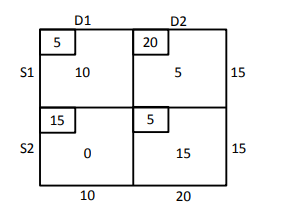
\includegraphics[width=0.75\columnwidth]{chapters/10/7/2/4/figs/fig.png}
 \end{center}
\caption{}
\label{fig:10/7/2/4Fig1}
\end{figure}
\fi

\item Find the position vector of the mid point of the vector joining the points $\vec{P}$(2, 3, 4)
and $\vec{Q}$(4, 1, –2).
\\
\solution
		\begin{enumerate}[label=\thesubsection.\arabic*,ref=\thesubsection.\theenumi]
\item Find the coordinates of the point which divides the join of $(-1,7) $ and $ (4,-3)$ in the ratio 2:3.
	\\
		\solution
	\input{chapters/10/7/2/1/section.tex}
\item Find the coordinates of the point $\vec{R}$ on the line segment joining the points $\vec{P}(-1,3)$ and $\vec{Q}(2,5)$ such that $PR=\frac{3}{5}PQ$.
\item Find the ratio in which the point $\vec{P}\brak{\frac{3}{4},\frac{5}{12}}$ divides the line segment joining the points $\vec{A}\brak{\frac{1}{2},\frac{3}{2}}$ and $ \vec{B}(2,-5)$.
\item Find the coordinates of the point which divides the line segment joining the points $(4,-3)$ and $(8,5)$ in the ratio $3:1$ internally.
\item Find the coordinates of the point $\vec{P}$ on $AD$ such that $AP : PD = 2 : 1$.
\item If the point $\vec{P} (2, 1)$ lies on the line segment joining points $\vec{A} (4, 2)$  and $ \vec{B} (8, 4)$,
then
\begin{enumerate}
	\item $AP =\frac{1}{3}{AB}$ 
\item ${AP}={PE}$
\item ${PB}=\frac{1}{3}{AB}$
\item${AP}=\frac{1}{2}{AB}$
 \end{enumerate}
\item Find the ratio in which the line segment joining the points $(-3,10)$  and  $(6,-8)$  is divided by $ (-1,6)$.
	\\
		\solution
	\input{chapters/10/7/2/4/section.tex}
\item Find the position vector of the mid point of the vector joining the points $\vec{P}$(2, 3, 4)
and $\vec{Q}$(4, 1, –2).
\\
\solution
		\input{chapters/12/10/2/16/section.tex}
\item Let $\vec{A}(4, 2), \vec{B}(6, 5)$  and $ \vec{C}(1, 4)$ be the vertices of $\triangle ABC$.
\begin{enumerate}
\item If $\vec{A}$ and  $\vec{B}$ are $(-2,-2)$ and  $(2,-4)$, respectively, find the coordinates of $\vec{P}$ such that $AP= \frac {3}{7}AB$  and $ \vec{P}$ lies on the line segment $AB$.
	\\
		\solution
	\input{chapters/10/7/2/8/section.tex}
\item Find the coordinates of the points which divide the line segment joining $A(-2,2)$  and  $\vec{B}(2,8)$ into four equal parts.
	\\
		\solution
	\input{chapters/10/7/2/9/section.tex}
\item In what ratio does the point $(-4,6)$ divide the line segment joining the points $\vec{A}(-6,0)$ and $\vec{B}(3,-8)$?
\item Given that $\vec{P}(3,2,-4), \vec{Q}(5,4,-6)$ and $\vec{R}(9,8,-10)$ are collinear. Find the ratio in which $\vec{Q}$ divides $PR$.
\item Points $\vec{A}(-6,10),\vec{B}(-4,6)$  and  $\vec{C}(3,-8)$ are collinear such that $AB=  \frac{2}{9}AC$.
\item The point which divides the line segment joining the points $\vec{P} (7, –6) $  and  $\vec{Q}(3, 4)$ in the 
ratio 1 : 2 internally lies in  which quadrant?
\item Find the coordinates of the points of trisection of the line segment joining $(4,-1)$  and  $(-2,3)$.
	\\
		\solution
	\input{chapters/10/7/2/2/section.tex}
\item Find the coordinates of the points which trisect the line segment joining the points $\vec{P}(4,2,-6)$ and $\vec{Q}(10,-16,6)$.
\item Find the coordinates of the points of trisection (i.e. points dividing to three equal parts) of the line segment joining the points $\vec{A}(2,-2)$ and $\vec{B}(-7,4)$.
\item Point $\vec{P}(5,-3)$ is one of the two points of trisection of line segment joining the points $\vec{A}(7,-2)$ and $\vec{B}(1,-5)$
\item Find the position vector of a point $\vec{R}$ which divides the line joining two points $\vec{P}$
and $\vec{Q}$ whose position vectors are $\hat{i}+2\hat{j}-\hat{k}$ and $-\hat{i}+\hat{j}+\hat{k}$ respectively, in the
ratio 2 : 1
\begin{enumerate}
    \item  internally
    \item  externally
\end{enumerate}
%\solution
%		\input{chapters/12/10/2/15/section.tex}
\item Find the coordinates of the point which divides the line segment joining the points which divides the line segment joining  the points $(-2,3,5)$ and $(1,-4,6)$ in the ratio 
\begin{enumerate}
\item $2:3$ internally,
\item $2:3$ externally
\end{enumerate}
\item Find the coordinates of the point which divides the line segment joining the points $(1,-2,3)$ and $(3,4,-5)$ in the ratio $2:3$
\begin{enumerate}
\item internally, and
\item externally
\end{enumerate}
\item Consider two points $\vec{P}$ and $\vec{Q}$ with position vectors $\overrightarrow{OP} = 3\overrightarrow{a}-2\overrightarrow{b}$ and $\overrightarrow{OQ}=\overrightarrow{a}+\overrightarrow{b}$. Find the position vector of a point $\vec{R}$ which divides the line joining $\vec{P}$ and $\vec{Q}$ in the ratio $2:1$, 
\begin{enumerate}
\item internally, and 
\item externally.
\end{enumerate}
\item The median from $\vec{A}$ meets $BC$ at $\vec{D}$. Find the coordinates of the point $\vec{D}$.
\item Find the coordinates of points $\vec{Q}$ and $\vec{R}$ on medians $BE$ and $CF$ respectively such that $BQ : QE = 2 : 1$  and  $CR : RF = 2 : 1$.
\item What do you observe?
\item If $\vec{A}, \vec{B}$ and $\vec{C}$  are the vertices of $\triangle ABC$, find the coordinates of the centroid of the triangle.
\end{enumerate}
\solution
	\input{chapters/10/7/4/7/section.tex}
\item If $\vec{P}(9a-2,-b)$ divides line segment joining $\vec{A}(3a+1,-3)$ and $\vec{B}(8a,5)$ in the ratio 3:1, find the values of $a$ and $b$.
\item Find the position vector of a point $\vec{R}$ which divides the line joining two points $\vec{P}$ and $\vec{Q}$ whose position vectors are $2\vec{a}+\vec{b}$ and $\vec{a}-3\vec{b}$ externally in the ratio $1:2$.
\item The position vector of the point which divides the join of points 2$\vec{a}$-3$\vec{b}$ $\text{and}$ $\vec{a}+\vec{b}$ in the ratio 3:1 is \rule{1cm}{0.1pt}.
\item If $\vec{a}$ and $\vec{b}$ are the postion vectors of $\vec{A}$ and $\vec{B}$, respectively, find the position vector of a point $\vec{C}$ in $BA$ produced such that $BC=1.5BA$.
\item Find the position vector of a point $\vec{R}$ which divides the line joining two points $\vec{P}$ and $\vec{Q}$ whose position vectors are $(2\vec{a}+\vec{b})$ and $(\vec{a}-3\vec{b})$
externally in the ratio 1 : 2. Also, show that $\vec{P}$ is the mid point of the line segment $RQ$.
\end{enumerate}

\item Let $\vec{A}(4, 2), \vec{B}(6, 5)$  and $ \vec{C}(1, 4)$ be the vertices of $\triangle ABC$.
\begin{enumerate}
\item If $\vec{A}$ and  $\vec{B}$ are $(-2,-2)$ and  $(2,-4)$, respectively, find the coordinates of $\vec{P}$ such that $AP= \frac {3}{7}AB$  and $ \vec{P}$ lies on the line segment $AB$.
	\\
		\solution
	\begin{enumerate}[label=\thesubsection.\arabic*,ref=\thesubsection.\theenumi]
\item Find the coordinates of the point which divides the join of $(-1,7) $ and $ (4,-3)$ in the ratio 2:3.
	\\
		\solution
	\input{chapters/10/7/2/1/section.tex}
\item Find the coordinates of the point $\vec{R}$ on the line segment joining the points $\vec{P}(-1,3)$ and $\vec{Q}(2,5)$ such that $PR=\frac{3}{5}PQ$.
\item Find the ratio in which the point $\vec{P}\brak{\frac{3}{4},\frac{5}{12}}$ divides the line segment joining the points $\vec{A}\brak{\frac{1}{2},\frac{3}{2}}$ and $ \vec{B}(2,-5)$.
\item Find the coordinates of the point which divides the line segment joining the points $(4,-3)$ and $(8,5)$ in the ratio $3:1$ internally.
\item Find the coordinates of the point $\vec{P}$ on $AD$ such that $AP : PD = 2 : 1$.
\item If the point $\vec{P} (2, 1)$ lies on the line segment joining points $\vec{A} (4, 2)$  and $ \vec{B} (8, 4)$,
then
\begin{enumerate}
	\item $AP =\frac{1}{3}{AB}$ 
\item ${AP}={PE}$
\item ${PB}=\frac{1}{3}{AB}$
\item${AP}=\frac{1}{2}{AB}$
 \end{enumerate}
\item Find the ratio in which the line segment joining the points $(-3,10)$  and  $(6,-8)$  is divided by $ (-1,6)$.
	\\
		\solution
	\input{chapters/10/7/2/4/section.tex}
\item Find the position vector of the mid point of the vector joining the points $\vec{P}$(2, 3, 4)
and $\vec{Q}$(4, 1, –2).
\\
\solution
		\input{chapters/12/10/2/16/section.tex}
\item Let $\vec{A}(4, 2), \vec{B}(6, 5)$  and $ \vec{C}(1, 4)$ be the vertices of $\triangle ABC$.
\begin{enumerate}
\item If $\vec{A}$ and  $\vec{B}$ are $(-2,-2)$ and  $(2,-4)$, respectively, find the coordinates of $\vec{P}$ such that $AP= \frac {3}{7}AB$  and $ \vec{P}$ lies on the line segment $AB$.
	\\
		\solution
	\input{chapters/10/7/2/8/section.tex}
\item Find the coordinates of the points which divide the line segment joining $A(-2,2)$  and  $\vec{B}(2,8)$ into four equal parts.
	\\
		\solution
	\input{chapters/10/7/2/9/section.tex}
\item In what ratio does the point $(-4,6)$ divide the line segment joining the points $\vec{A}(-6,0)$ and $\vec{B}(3,-8)$?
\item Given that $\vec{P}(3,2,-4), \vec{Q}(5,4,-6)$ and $\vec{R}(9,8,-10)$ are collinear. Find the ratio in which $\vec{Q}$ divides $PR$.
\item Points $\vec{A}(-6,10),\vec{B}(-4,6)$  and  $\vec{C}(3,-8)$ are collinear such that $AB=  \frac{2}{9}AC$.
\item The point which divides the line segment joining the points $\vec{P} (7, –6) $  and  $\vec{Q}(3, 4)$ in the 
ratio 1 : 2 internally lies in  which quadrant?
\item Find the coordinates of the points of trisection of the line segment joining $(4,-1)$  and  $(-2,3)$.
	\\
		\solution
	\input{chapters/10/7/2/2/section.tex}
\item Find the coordinates of the points which trisect the line segment joining the points $\vec{P}(4,2,-6)$ and $\vec{Q}(10,-16,6)$.
\item Find the coordinates of the points of trisection (i.e. points dividing to three equal parts) of the line segment joining the points $\vec{A}(2,-2)$ and $\vec{B}(-7,4)$.
\item Point $\vec{P}(5,-3)$ is one of the two points of trisection of line segment joining the points $\vec{A}(7,-2)$ and $\vec{B}(1,-5)$
\item Find the position vector of a point $\vec{R}$ which divides the line joining two points $\vec{P}$
and $\vec{Q}$ whose position vectors are $\hat{i}+2\hat{j}-\hat{k}$ and $-\hat{i}+\hat{j}+\hat{k}$ respectively, in the
ratio 2 : 1
\begin{enumerate}
    \item  internally
    \item  externally
\end{enumerate}
%\solution
%		\input{chapters/12/10/2/15/section.tex}
\item Find the coordinates of the point which divides the line segment joining the points which divides the line segment joining  the points $(-2,3,5)$ and $(1,-4,6)$ in the ratio 
\begin{enumerate}
\item $2:3$ internally,
\item $2:3$ externally
\end{enumerate}
\item Find the coordinates of the point which divides the line segment joining the points $(1,-2,3)$ and $(3,4,-5)$ in the ratio $2:3$
\begin{enumerate}
\item internally, and
\item externally
\end{enumerate}
\item Consider two points $\vec{P}$ and $\vec{Q}$ with position vectors $\overrightarrow{OP} = 3\overrightarrow{a}-2\overrightarrow{b}$ and $\overrightarrow{OQ}=\overrightarrow{a}+\overrightarrow{b}$. Find the position vector of a point $\vec{R}$ which divides the line joining $\vec{P}$ and $\vec{Q}$ in the ratio $2:1$, 
\begin{enumerate}
\item internally, and 
\item externally.
\end{enumerate}
\item The median from $\vec{A}$ meets $BC$ at $\vec{D}$. Find the coordinates of the point $\vec{D}$.
\item Find the coordinates of points $\vec{Q}$ and $\vec{R}$ on medians $BE$ and $CF$ respectively such that $BQ : QE = 2 : 1$  and  $CR : RF = 2 : 1$.
\item What do you observe?
\item If $\vec{A}, \vec{B}$ and $\vec{C}$  are the vertices of $\triangle ABC$, find the coordinates of the centroid of the triangle.
\end{enumerate}
\solution
	\input{chapters/10/7/4/7/section.tex}
\item If $\vec{P}(9a-2,-b)$ divides line segment joining $\vec{A}(3a+1,-3)$ and $\vec{B}(8a,5)$ in the ratio 3:1, find the values of $a$ and $b$.
\item Find the position vector of a point $\vec{R}$ which divides the line joining two points $\vec{P}$ and $\vec{Q}$ whose position vectors are $2\vec{a}+\vec{b}$ and $\vec{a}-3\vec{b}$ externally in the ratio $1:2$.
\item The position vector of the point which divides the join of points 2$\vec{a}$-3$\vec{b}$ $\text{and}$ $\vec{a}+\vec{b}$ in the ratio 3:1 is \rule{1cm}{0.1pt}.
\item If $\vec{a}$ and $\vec{b}$ are the postion vectors of $\vec{A}$ and $\vec{B}$, respectively, find the position vector of a point $\vec{C}$ in $BA$ produced such that $BC=1.5BA$.
\item Find the position vector of a point $\vec{R}$ which divides the line joining two points $\vec{P}$ and $\vec{Q}$ whose position vectors are $(2\vec{a}+\vec{b})$ and $(\vec{a}-3\vec{b})$
externally in the ratio 1 : 2. Also, show that $\vec{P}$ is the mid point of the line segment $RQ$.
\end{enumerate}

\item Find the coordinates of the points which divide the line segment joining $A(-2,2)$  and  $\vec{B}(2,8)$ into four equal parts.
	\\
		\solution
	\begin{enumerate}[label=\thesubsection.\arabic*,ref=\thesubsection.\theenumi]
\item Find the coordinates of the point which divides the join of $(-1,7) $ and $ (4,-3)$ in the ratio 2:3.
	\\
		\solution
	\input{chapters/10/7/2/1/section.tex}
\item Find the coordinates of the point $\vec{R}$ on the line segment joining the points $\vec{P}(-1,3)$ and $\vec{Q}(2,5)$ such that $PR=\frac{3}{5}PQ$.
\item Find the ratio in which the point $\vec{P}\brak{\frac{3}{4},\frac{5}{12}}$ divides the line segment joining the points $\vec{A}\brak{\frac{1}{2},\frac{3}{2}}$ and $ \vec{B}(2,-5)$.
\item Find the coordinates of the point which divides the line segment joining the points $(4,-3)$ and $(8,5)$ in the ratio $3:1$ internally.
\item Find the coordinates of the point $\vec{P}$ on $AD$ such that $AP : PD = 2 : 1$.
\item If the point $\vec{P} (2, 1)$ lies on the line segment joining points $\vec{A} (4, 2)$  and $ \vec{B} (8, 4)$,
then
\begin{enumerate}
	\item $AP =\frac{1}{3}{AB}$ 
\item ${AP}={PE}$
\item ${PB}=\frac{1}{3}{AB}$
\item${AP}=\frac{1}{2}{AB}$
 \end{enumerate}
\item Find the ratio in which the line segment joining the points $(-3,10)$  and  $(6,-8)$  is divided by $ (-1,6)$.
	\\
		\solution
	\input{chapters/10/7/2/4/section.tex}
\item Find the position vector of the mid point of the vector joining the points $\vec{P}$(2, 3, 4)
and $\vec{Q}$(4, 1, –2).
\\
\solution
		\input{chapters/12/10/2/16/section.tex}
\item Let $\vec{A}(4, 2), \vec{B}(6, 5)$  and $ \vec{C}(1, 4)$ be the vertices of $\triangle ABC$.
\begin{enumerate}
\item If $\vec{A}$ and  $\vec{B}$ are $(-2,-2)$ and  $(2,-4)$, respectively, find the coordinates of $\vec{P}$ such that $AP= \frac {3}{7}AB$  and $ \vec{P}$ lies on the line segment $AB$.
	\\
		\solution
	\input{chapters/10/7/2/8/section.tex}
\item Find the coordinates of the points which divide the line segment joining $A(-2,2)$  and  $\vec{B}(2,8)$ into four equal parts.
	\\
		\solution
	\input{chapters/10/7/2/9/section.tex}
\item In what ratio does the point $(-4,6)$ divide the line segment joining the points $\vec{A}(-6,0)$ and $\vec{B}(3,-8)$?
\item Given that $\vec{P}(3,2,-4), \vec{Q}(5,4,-6)$ and $\vec{R}(9,8,-10)$ are collinear. Find the ratio in which $\vec{Q}$ divides $PR$.
\item Points $\vec{A}(-6,10),\vec{B}(-4,6)$  and  $\vec{C}(3,-8)$ are collinear such that $AB=  \frac{2}{9}AC$.
\item The point which divides the line segment joining the points $\vec{P} (7, –6) $  and  $\vec{Q}(3, 4)$ in the 
ratio 1 : 2 internally lies in  which quadrant?
\item Find the coordinates of the points of trisection of the line segment joining $(4,-1)$  and  $(-2,3)$.
	\\
		\solution
	\input{chapters/10/7/2/2/section.tex}
\item Find the coordinates of the points which trisect the line segment joining the points $\vec{P}(4,2,-6)$ and $\vec{Q}(10,-16,6)$.
\item Find the coordinates of the points of trisection (i.e. points dividing to three equal parts) of the line segment joining the points $\vec{A}(2,-2)$ and $\vec{B}(-7,4)$.
\item Point $\vec{P}(5,-3)$ is one of the two points of trisection of line segment joining the points $\vec{A}(7,-2)$ and $\vec{B}(1,-5)$
\item Find the position vector of a point $\vec{R}$ which divides the line joining two points $\vec{P}$
and $\vec{Q}$ whose position vectors are $\hat{i}+2\hat{j}-\hat{k}$ and $-\hat{i}+\hat{j}+\hat{k}$ respectively, in the
ratio 2 : 1
\begin{enumerate}
    \item  internally
    \item  externally
\end{enumerate}
%\solution
%		\input{chapters/12/10/2/15/section.tex}
\item Find the coordinates of the point which divides the line segment joining the points which divides the line segment joining  the points $(-2,3,5)$ and $(1,-4,6)$ in the ratio 
\begin{enumerate}
\item $2:3$ internally,
\item $2:3$ externally
\end{enumerate}
\item Find the coordinates of the point which divides the line segment joining the points $(1,-2,3)$ and $(3,4,-5)$ in the ratio $2:3$
\begin{enumerate}
\item internally, and
\item externally
\end{enumerate}
\item Consider two points $\vec{P}$ and $\vec{Q}$ with position vectors $\overrightarrow{OP} = 3\overrightarrow{a}-2\overrightarrow{b}$ and $\overrightarrow{OQ}=\overrightarrow{a}+\overrightarrow{b}$. Find the position vector of a point $\vec{R}$ which divides the line joining $\vec{P}$ and $\vec{Q}$ in the ratio $2:1$, 
\begin{enumerate}
\item internally, and 
\item externally.
\end{enumerate}
\item The median from $\vec{A}$ meets $BC$ at $\vec{D}$. Find the coordinates of the point $\vec{D}$.
\item Find the coordinates of points $\vec{Q}$ and $\vec{R}$ on medians $BE$ and $CF$ respectively such that $BQ : QE = 2 : 1$  and  $CR : RF = 2 : 1$.
\item What do you observe?
\item If $\vec{A}, \vec{B}$ and $\vec{C}$  are the vertices of $\triangle ABC$, find the coordinates of the centroid of the triangle.
\end{enumerate}
\solution
	\input{chapters/10/7/4/7/section.tex}
\item If $\vec{P}(9a-2,-b)$ divides line segment joining $\vec{A}(3a+1,-3)$ and $\vec{B}(8a,5)$ in the ratio 3:1, find the values of $a$ and $b$.
\item Find the position vector of a point $\vec{R}$ which divides the line joining two points $\vec{P}$ and $\vec{Q}$ whose position vectors are $2\vec{a}+\vec{b}$ and $\vec{a}-3\vec{b}$ externally in the ratio $1:2$.
\item The position vector of the point which divides the join of points 2$\vec{a}$-3$\vec{b}$ $\text{and}$ $\vec{a}+\vec{b}$ in the ratio 3:1 is \rule{1cm}{0.1pt}.
\item If $\vec{a}$ and $\vec{b}$ are the postion vectors of $\vec{A}$ and $\vec{B}$, respectively, find the position vector of a point $\vec{C}$ in $BA$ produced such that $BC=1.5BA$.
\item Find the position vector of a point $\vec{R}$ which divides the line joining two points $\vec{P}$ and $\vec{Q}$ whose position vectors are $(2\vec{a}+\vec{b})$ and $(\vec{a}-3\vec{b})$
externally in the ratio 1 : 2. Also, show that $\vec{P}$ is the mid point of the line segment $RQ$.
\end{enumerate}

\item In what ratio does the point $(-4,6)$ divide the line segment joining the points $\vec{A}(-6,0)$ and $\vec{B}(3,-8)$?
\item Given that $\vec{P}(3,2,-4), \vec{Q}(5,4,-6)$ and $\vec{R}(9,8,-10)$ are collinear. Find the ratio in which $\vec{Q}$ divides $PR$.
\item Points $\vec{A}(-6,10),\vec{B}(-4,6)$  and  $\vec{C}(3,-8)$ are collinear such that $AB=  \frac{2}{9}AC$.
\item The point which divides the line segment joining the points $\vec{P} (7, –6) $  and  $\vec{Q}(3, 4)$ in the 
ratio 1 : 2 internally lies in  which quadrant?
\item Find the coordinates of the points of trisection of the line segment joining $(4,-1)$  and  $(-2,3)$.
	\\
		\solution
	Using section formula,
\begin{align}
\vec{R}=\frac{1}{1+\frac{1}{2}}\brak{\myvec{4\\-1}+\frac{1}{2}\myvec{-2\\3}}
=\myvec{2\\ \frac{1}{3}}\\
\vec{S}=\frac{1}{1+\frac{2}{1}}\brak{\myvec{4\\-1}+\frac{2}{1}\myvec{-2\\3}}
=\myvec{0\\ \frac{5}{3}}
\end{align}
which are the desired points of trisection.
\iffalse
See
		\figref{fig:chapters/10/7/2/2/Figure}
\begin{figure}[H]
\centering
\includegraphics[width=0.75\columnwidth]{chapters/10/7/2/2/figs/dj.pdf}
\caption{}
		\label{fig:chapters/10/7/2/2/Figure}
\end{figure}
\fi

\item Find the coordinates of the points which trisect the line segment joining the points $\vec{P}(4,2,-6)$ and $\vec{Q}(10,-16,6)$.
\item Find the coordinates of the points of trisection (i.e. points dividing to three equal parts) of the line segment joining the points $\vec{A}(2,-2)$ and $\vec{B}(-7,4)$.
\item Point $\vec{P}(5,-3)$ is one of the two points of trisection of line segment joining the points $\vec{A}(7,-2)$ and $\vec{B}(1,-5)$
\item Find the position vector of a point $\vec{R}$ which divides the line joining two points $\vec{P}$
and $\vec{Q}$ whose position vectors are $\hat{i}+2\hat{j}-\hat{k}$ and $-\hat{i}+\hat{j}+\hat{k}$ respectively, in the
ratio 2 : 1
\begin{enumerate}
    \item  internally
    \item  externally
\end{enumerate}
%\solution
%		\begin{enumerate}[label=\thesubsection.\arabic*,ref=\thesubsection.\theenumi]
\item Find the coordinates of the point which divides the join of $(-1,7) $ and $ (4,-3)$ in the ratio 2:3.
	\\
		\solution
	\input{chapters/10/7/2/1/section.tex}
\item Find the coordinates of the point $\vec{R}$ on the line segment joining the points $\vec{P}(-1,3)$ and $\vec{Q}(2,5)$ such that $PR=\frac{3}{5}PQ$.
\item Find the ratio in which the point $\vec{P}\brak{\frac{3}{4},\frac{5}{12}}$ divides the line segment joining the points $\vec{A}\brak{\frac{1}{2},\frac{3}{2}}$ and $ \vec{B}(2,-5)$.
\item Find the coordinates of the point which divides the line segment joining the points $(4,-3)$ and $(8,5)$ in the ratio $3:1$ internally.
\item Find the coordinates of the point $\vec{P}$ on $AD$ such that $AP : PD = 2 : 1$.
\item If the point $\vec{P} (2, 1)$ lies on the line segment joining points $\vec{A} (4, 2)$  and $ \vec{B} (8, 4)$,
then
\begin{enumerate}
	\item $AP =\frac{1}{3}{AB}$ 
\item ${AP}={PE}$
\item ${PB}=\frac{1}{3}{AB}$
\item${AP}=\frac{1}{2}{AB}$
 \end{enumerate}
\item Find the ratio in which the line segment joining the points $(-3,10)$  and  $(6,-8)$  is divided by $ (-1,6)$.
	\\
		\solution
	\input{chapters/10/7/2/4/section.tex}
\item Find the position vector of the mid point of the vector joining the points $\vec{P}$(2, 3, 4)
and $\vec{Q}$(4, 1, –2).
\\
\solution
		\input{chapters/12/10/2/16/section.tex}
\item Let $\vec{A}(4, 2), \vec{B}(6, 5)$  and $ \vec{C}(1, 4)$ be the vertices of $\triangle ABC$.
\begin{enumerate}
\item If $\vec{A}$ and  $\vec{B}$ are $(-2,-2)$ and  $(2,-4)$, respectively, find the coordinates of $\vec{P}$ such that $AP= \frac {3}{7}AB$  and $ \vec{P}$ lies on the line segment $AB$.
	\\
		\solution
	\input{chapters/10/7/2/8/section.tex}
\item Find the coordinates of the points which divide the line segment joining $A(-2,2)$  and  $\vec{B}(2,8)$ into four equal parts.
	\\
		\solution
	\input{chapters/10/7/2/9/section.tex}
\item In what ratio does the point $(-4,6)$ divide the line segment joining the points $\vec{A}(-6,0)$ and $\vec{B}(3,-8)$?
\item Given that $\vec{P}(3,2,-4), \vec{Q}(5,4,-6)$ and $\vec{R}(9,8,-10)$ are collinear. Find the ratio in which $\vec{Q}$ divides $PR$.
\item Points $\vec{A}(-6,10),\vec{B}(-4,6)$  and  $\vec{C}(3,-8)$ are collinear such that $AB=  \frac{2}{9}AC$.
\item The point which divides the line segment joining the points $\vec{P} (7, –6) $  and  $\vec{Q}(3, 4)$ in the 
ratio 1 : 2 internally lies in  which quadrant?
\item Find the coordinates of the points of trisection of the line segment joining $(4,-1)$  and  $(-2,3)$.
	\\
		\solution
	\input{chapters/10/7/2/2/section.tex}
\item Find the coordinates of the points which trisect the line segment joining the points $\vec{P}(4,2,-6)$ and $\vec{Q}(10,-16,6)$.
\item Find the coordinates of the points of trisection (i.e. points dividing to three equal parts) of the line segment joining the points $\vec{A}(2,-2)$ and $\vec{B}(-7,4)$.
\item Point $\vec{P}(5,-3)$ is one of the two points of trisection of line segment joining the points $\vec{A}(7,-2)$ and $\vec{B}(1,-5)$
\item Find the position vector of a point $\vec{R}$ which divides the line joining two points $\vec{P}$
and $\vec{Q}$ whose position vectors are $\hat{i}+2\hat{j}-\hat{k}$ and $-\hat{i}+\hat{j}+\hat{k}$ respectively, in the
ratio 2 : 1
\begin{enumerate}
    \item  internally
    \item  externally
\end{enumerate}
%\solution
%		\input{chapters/12/10/2/15/section.tex}
\item Find the coordinates of the point which divides the line segment joining the points which divides the line segment joining  the points $(-2,3,5)$ and $(1,-4,6)$ in the ratio 
\begin{enumerate}
\item $2:3$ internally,
\item $2:3$ externally
\end{enumerate}
\item Find the coordinates of the point which divides the line segment joining the points $(1,-2,3)$ and $(3,4,-5)$ in the ratio $2:3$
\begin{enumerate}
\item internally, and
\item externally
\end{enumerate}
\item Consider two points $\vec{P}$ and $\vec{Q}$ with position vectors $\overrightarrow{OP} = 3\overrightarrow{a}-2\overrightarrow{b}$ and $\overrightarrow{OQ}=\overrightarrow{a}+\overrightarrow{b}$. Find the position vector of a point $\vec{R}$ which divides the line joining $\vec{P}$ and $\vec{Q}$ in the ratio $2:1$, 
\begin{enumerate}
\item internally, and 
\item externally.
\end{enumerate}
\item The median from $\vec{A}$ meets $BC$ at $\vec{D}$. Find the coordinates of the point $\vec{D}$.
\item Find the coordinates of points $\vec{Q}$ and $\vec{R}$ on medians $BE$ and $CF$ respectively such that $BQ : QE = 2 : 1$  and  $CR : RF = 2 : 1$.
\item What do you observe?
\item If $\vec{A}, \vec{B}$ and $\vec{C}$  are the vertices of $\triangle ABC$, find the coordinates of the centroid of the triangle.
\end{enumerate}
\solution
	\input{chapters/10/7/4/7/section.tex}
\item If $\vec{P}(9a-2,-b)$ divides line segment joining $\vec{A}(3a+1,-3)$ and $\vec{B}(8a,5)$ in the ratio 3:1, find the values of $a$ and $b$.
\item Find the position vector of a point $\vec{R}$ which divides the line joining two points $\vec{P}$ and $\vec{Q}$ whose position vectors are $2\vec{a}+\vec{b}$ and $\vec{a}-3\vec{b}$ externally in the ratio $1:2$.
\item The position vector of the point which divides the join of points 2$\vec{a}$-3$\vec{b}$ $\text{and}$ $\vec{a}+\vec{b}$ in the ratio 3:1 is \rule{1cm}{0.1pt}.
\item If $\vec{a}$ and $\vec{b}$ are the postion vectors of $\vec{A}$ and $\vec{B}$, respectively, find the position vector of a point $\vec{C}$ in $BA$ produced such that $BC=1.5BA$.
\item Find the position vector of a point $\vec{R}$ which divides the line joining two points $\vec{P}$ and $\vec{Q}$ whose position vectors are $(2\vec{a}+\vec{b})$ and $(\vec{a}-3\vec{b})$
externally in the ratio 1 : 2. Also, show that $\vec{P}$ is the mid point of the line segment $RQ$.
\end{enumerate}

\item Find the coordinates of the point which divides the line segment joining the points which divides the line segment joining  the points $(-2,3,5)$ and $(1,-4,6)$ in the ratio 
\begin{enumerate}
\item $2:3$ internally,
\item $2:3$ externally
\end{enumerate}
\item Find the coordinates of the point which divides the line segment joining the points $(1,-2,3)$ and $(3,4,-5)$ in the ratio $2:3$
\begin{enumerate}
\item internally, and
\item externally
\end{enumerate}
\item Consider two points $\vec{P}$ and $\vec{Q}$ with position vectors $\overrightarrow{OP} = 3\overrightarrow{a}-2\overrightarrow{b}$ and $\overrightarrow{OQ}=\overrightarrow{a}+\overrightarrow{b}$. Find the position vector of a point $\vec{R}$ which divides the line joining $\vec{P}$ and $\vec{Q}$ in the ratio $2:1$, 
\begin{enumerate}
\item internally, and 
\item externally.
\end{enumerate}
\item The median from $\vec{A}$ meets $BC$ at $\vec{D}$. Find the coordinates of the point $\vec{D}$.
\item Find the coordinates of points $\vec{Q}$ and $\vec{R}$ on medians $BE$ and $CF$ respectively such that $BQ : QE = 2 : 1$  and  $CR : RF = 2 : 1$.
\item What do you observe?
\item If $\vec{A}, \vec{B}$ and $\vec{C}$  are the vertices of $\triangle ABC$, find the coordinates of the centroid of the triangle.
\end{enumerate}
\solution
	\begin{enumerate}[label=\thesubsection.\arabic*,ref=\thesubsection.\theenumi]
\item Find the coordinates of the point which divides the join of $(-1,7) $ and $ (4,-3)$ in the ratio 2:3.
	\\
		\solution
	\input{chapters/10/7/2/1/section.tex}
\item Find the coordinates of the point $\vec{R}$ on the line segment joining the points $\vec{P}(-1,3)$ and $\vec{Q}(2,5)$ such that $PR=\frac{3}{5}PQ$.
\item Find the ratio in which the point $\vec{P}\brak{\frac{3}{4},\frac{5}{12}}$ divides the line segment joining the points $\vec{A}\brak{\frac{1}{2},\frac{3}{2}}$ and $ \vec{B}(2,-5)$.
\item Find the coordinates of the point which divides the line segment joining the points $(4,-3)$ and $(8,5)$ in the ratio $3:1$ internally.
\item Find the coordinates of the point $\vec{P}$ on $AD$ such that $AP : PD = 2 : 1$.
\item If the point $\vec{P} (2, 1)$ lies on the line segment joining points $\vec{A} (4, 2)$  and $ \vec{B} (8, 4)$,
then
\begin{enumerate}
	\item $AP =\frac{1}{3}{AB}$ 
\item ${AP}={PE}$
\item ${PB}=\frac{1}{3}{AB}$
\item${AP}=\frac{1}{2}{AB}$
 \end{enumerate}
\item Find the ratio in which the line segment joining the points $(-3,10)$  and  $(6,-8)$  is divided by $ (-1,6)$.
	\\
		\solution
	\input{chapters/10/7/2/4/section.tex}
\item Find the position vector of the mid point of the vector joining the points $\vec{P}$(2, 3, 4)
and $\vec{Q}$(4, 1, –2).
\\
\solution
		\input{chapters/12/10/2/16/section.tex}
\item Let $\vec{A}(4, 2), \vec{B}(6, 5)$  and $ \vec{C}(1, 4)$ be the vertices of $\triangle ABC$.
\begin{enumerate}
\item If $\vec{A}$ and  $\vec{B}$ are $(-2,-2)$ and  $(2,-4)$, respectively, find the coordinates of $\vec{P}$ such that $AP= \frac {3}{7}AB$  and $ \vec{P}$ lies on the line segment $AB$.
	\\
		\solution
	\input{chapters/10/7/2/8/section.tex}
\item Find the coordinates of the points which divide the line segment joining $A(-2,2)$  and  $\vec{B}(2,8)$ into four equal parts.
	\\
		\solution
	\input{chapters/10/7/2/9/section.tex}
\item In what ratio does the point $(-4,6)$ divide the line segment joining the points $\vec{A}(-6,0)$ and $\vec{B}(3,-8)$?
\item Given that $\vec{P}(3,2,-4), \vec{Q}(5,4,-6)$ and $\vec{R}(9,8,-10)$ are collinear. Find the ratio in which $\vec{Q}$ divides $PR$.
\item Points $\vec{A}(-6,10),\vec{B}(-4,6)$  and  $\vec{C}(3,-8)$ are collinear such that $AB=  \frac{2}{9}AC$.
\item The point which divides the line segment joining the points $\vec{P} (7, –6) $  and  $\vec{Q}(3, 4)$ in the 
ratio 1 : 2 internally lies in  which quadrant?
\item Find the coordinates of the points of trisection of the line segment joining $(4,-1)$  and  $(-2,3)$.
	\\
		\solution
	\input{chapters/10/7/2/2/section.tex}
\item Find the coordinates of the points which trisect the line segment joining the points $\vec{P}(4,2,-6)$ and $\vec{Q}(10,-16,6)$.
\item Find the coordinates of the points of trisection (i.e. points dividing to three equal parts) of the line segment joining the points $\vec{A}(2,-2)$ and $\vec{B}(-7,4)$.
\item Point $\vec{P}(5,-3)$ is one of the two points of trisection of line segment joining the points $\vec{A}(7,-2)$ and $\vec{B}(1,-5)$
\item Find the position vector of a point $\vec{R}$ which divides the line joining two points $\vec{P}$
and $\vec{Q}$ whose position vectors are $\hat{i}+2\hat{j}-\hat{k}$ and $-\hat{i}+\hat{j}+\hat{k}$ respectively, in the
ratio 2 : 1
\begin{enumerate}
    \item  internally
    \item  externally
\end{enumerate}
%\solution
%		\input{chapters/12/10/2/15/section.tex}
\item Find the coordinates of the point which divides the line segment joining the points which divides the line segment joining  the points $(-2,3,5)$ and $(1,-4,6)$ in the ratio 
\begin{enumerate}
\item $2:3$ internally,
\item $2:3$ externally
\end{enumerate}
\item Find the coordinates of the point which divides the line segment joining the points $(1,-2,3)$ and $(3,4,-5)$ in the ratio $2:3$
\begin{enumerate}
\item internally, and
\item externally
\end{enumerate}
\item Consider two points $\vec{P}$ and $\vec{Q}$ with position vectors $\overrightarrow{OP} = 3\overrightarrow{a}-2\overrightarrow{b}$ and $\overrightarrow{OQ}=\overrightarrow{a}+\overrightarrow{b}$. Find the position vector of a point $\vec{R}$ which divides the line joining $\vec{P}$ and $\vec{Q}$ in the ratio $2:1$, 
\begin{enumerate}
\item internally, and 
\item externally.
\end{enumerate}
\item The median from $\vec{A}$ meets $BC$ at $\vec{D}$. Find the coordinates of the point $\vec{D}$.
\item Find the coordinates of points $\vec{Q}$ and $\vec{R}$ on medians $BE$ and $CF$ respectively such that $BQ : QE = 2 : 1$  and  $CR : RF = 2 : 1$.
\item What do you observe?
\item If $\vec{A}, \vec{B}$ and $\vec{C}$  are the vertices of $\triangle ABC$, find the coordinates of the centroid of the triangle.
\end{enumerate}
\solution
	\input{chapters/10/7/4/7/section.tex}
\item If $\vec{P}(9a-2,-b)$ divides line segment joining $\vec{A}(3a+1,-3)$ and $\vec{B}(8a,5)$ in the ratio 3:1, find the values of $a$ and $b$.
\item Find the position vector of a point $\vec{R}$ which divides the line joining two points $\vec{P}$ and $\vec{Q}$ whose position vectors are $2\vec{a}+\vec{b}$ and $\vec{a}-3\vec{b}$ externally in the ratio $1:2$.
\item The position vector of the point which divides the join of points 2$\vec{a}$-3$\vec{b}$ $\text{and}$ $\vec{a}+\vec{b}$ in the ratio 3:1 is \rule{1cm}{0.1pt}.
\item If $\vec{a}$ and $\vec{b}$ are the postion vectors of $\vec{A}$ and $\vec{B}$, respectively, find the position vector of a point $\vec{C}$ in $BA$ produced such that $BC=1.5BA$.
\item Find the position vector of a point $\vec{R}$ which divides the line joining two points $\vec{P}$ and $\vec{Q}$ whose position vectors are $(2\vec{a}+\vec{b})$ and $(\vec{a}-3\vec{b})$
externally in the ratio 1 : 2. Also, show that $\vec{P}$ is the mid point of the line segment $RQ$.
\end{enumerate}

\item If $\vec{P}(9a-2,-b)$ divides line segment joining $\vec{A}(3a+1,-3)$ and $\vec{B}(8a,5)$ in the ratio 3:1, find the values of $a$ and $b$.
\item Find the position vector of a point $\vec{R}$ which divides the line joining two points $\vec{P}$ and $\vec{Q}$ whose position vectors are $2\vec{a}+\vec{b}$ and $\vec{a}-3\vec{b}$ externally in the ratio $1:2$.
\item The position vector of the point which divides the join of points 2$\vec{a}$-3$\vec{b}$ $\text{and}$ $\vec{a}+\vec{b}$ in the ratio 3:1 is \rule{1cm}{0.1pt}.
\item If $\vec{a}$ and $\vec{b}$ are the postion vectors of $\vec{A}$ and $\vec{B}$, respectively, find the position vector of a point $\vec{C}$ in $BA$ produced such that $BC=1.5BA$.
\item Find the position vector of a point $\vec{R}$ which divides the line joining two points $\vec{P}$ and $\vec{Q}$ whose position vectors are $(2\vec{a}+\vec{b})$ and $(\vec{a}-3\vec{b})$
externally in the ratio 1 : 2. Also, show that $\vec{P}$ is the mid point of the line segment $RQ$.
\end{enumerate}

\item Find the coordinates of the point $\vec{R}$ on the line segment joining the points $\vec{P}(-1,3)$ and $\vec{Q}(2,5)$ such that $PR=\frac{3}{5}PQ$.
\item Find the ratio in which the point $\vec{P}\brak{\frac{3}{4},\frac{5}{12}}$ divides the line segment joining the points $\vec{A}\brak{\frac{1}{2},\frac{3}{2}}$ and $ \vec{B}(2,-5)$.
\item Find the coordinates of the point which divides the line segment joining the points $(4,-3)$ and $(8,5)$ in the ratio $3:1$ internally.
\item Find the coordinates of the point $\vec{P}$ on $AD$ such that $AP : PD = 2 : 1$.
\item If the point $\vec{P} (2, 1)$ lies on the line segment joining points $\vec{A} (4, 2)$  and $ \vec{B} (8, 4)$,
then
\begin{enumerate}
	\item $AP =\frac{1}{3}{AB}$ 
\item ${AP}={PE}$
\item ${PB}=\frac{1}{3}{AB}$
\item${AP}=\frac{1}{2}{AB}$
 \end{enumerate}
\item Find the ratio in which the line segment joining the points $(-3,10)$  and  $(6,-8)$  is divided by $ (-1,6)$.
	\\
		\solution
	\iffalse
Using section formula,
\begin{align}
         \myvec{-1\\6} &=\frac{{\myvec{-3\\10}+k\myvec{6\\-8}}}{1+k}\\
	 \implies 7k\myvec{1 \\ -2} &= 2\myvec{1 \\ -2}
	 \\
	 \text{or, } k &= \frac{2}{7}.
\end{align}
\fi
In 
			\eqref{eq:section_formula-k}, substituting
			\begin{align}
				\vec{B} &= \myvec{-3\\10}, \vec{C} = \myvec{6\\-8}, \vec{D} = \myvec{-1\\6},
				\\
				k &= \frac{\myvec{-2 & 4}\myvec{-7 \\ 14}}{\norm{\myvec{-7 \\ 14}}^2} = \frac{2}{7}
			\end{align}
\iffalse
See \figref{fig:10/7/2/4Fig1}.
\begin{figure}[H]
 \begin{center}
  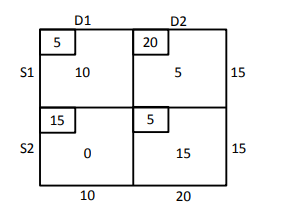
\includegraphics[width=0.75\columnwidth]{chapters/10/7/2/4/figs/fig.png}
 \end{center}
\caption{}
\label{fig:10/7/2/4Fig1}
\end{figure}
\fi

\item Find the position vector of the mid point of the vector joining the points $\vec{P}$(2, 3, 4)
and $\vec{Q}$(4, 1, –2).
\\
\solution
		\begin{enumerate}[label=\thesubsection.\arabic*,ref=\thesubsection.\theenumi]
\item Find the coordinates of the point which divides the join of $(-1,7) $ and $ (4,-3)$ in the ratio 2:3.
	\\
		\solution
	\begin{enumerate}[label=\thesubsection.\arabic*,ref=\thesubsection.\theenumi]
\item Find the coordinates of the point which divides the join of $(-1,7) $ and $ (4,-3)$ in the ratio 2:3.
	\\
		\solution
	\input{chapters/10/7/2/1/section.tex}
\item Find the coordinates of the point $\vec{R}$ on the line segment joining the points $\vec{P}(-1,3)$ and $\vec{Q}(2,5)$ such that $PR=\frac{3}{5}PQ$.
\item Find the ratio in which the point $\vec{P}\brak{\frac{3}{4},\frac{5}{12}}$ divides the line segment joining the points $\vec{A}\brak{\frac{1}{2},\frac{3}{2}}$ and $ \vec{B}(2,-5)$.
\item Find the coordinates of the point which divides the line segment joining the points $(4,-3)$ and $(8,5)$ in the ratio $3:1$ internally.
\item Find the coordinates of the point $\vec{P}$ on $AD$ such that $AP : PD = 2 : 1$.
\item If the point $\vec{P} (2, 1)$ lies on the line segment joining points $\vec{A} (4, 2)$  and $ \vec{B} (8, 4)$,
then
\begin{enumerate}
	\item $AP =\frac{1}{3}{AB}$ 
\item ${AP}={PE}$
\item ${PB}=\frac{1}{3}{AB}$
\item${AP}=\frac{1}{2}{AB}$
 \end{enumerate}
\item Find the ratio in which the line segment joining the points $(-3,10)$  and  $(6,-8)$  is divided by $ (-1,6)$.
	\\
		\solution
	\input{chapters/10/7/2/4/section.tex}
\item Find the position vector of the mid point of the vector joining the points $\vec{P}$(2, 3, 4)
and $\vec{Q}$(4, 1, –2).
\\
\solution
		\input{chapters/12/10/2/16/section.tex}
\item Let $\vec{A}(4, 2), \vec{B}(6, 5)$  and $ \vec{C}(1, 4)$ be the vertices of $\triangle ABC$.
\begin{enumerate}
\item If $\vec{A}$ and  $\vec{B}$ are $(-2,-2)$ and  $(2,-4)$, respectively, find the coordinates of $\vec{P}$ such that $AP= \frac {3}{7}AB$  and $ \vec{P}$ lies on the line segment $AB$.
	\\
		\solution
	\input{chapters/10/7/2/8/section.tex}
\item Find the coordinates of the points which divide the line segment joining $A(-2,2)$  and  $\vec{B}(2,8)$ into four equal parts.
	\\
		\solution
	\input{chapters/10/7/2/9/section.tex}
\item In what ratio does the point $(-4,6)$ divide the line segment joining the points $\vec{A}(-6,0)$ and $\vec{B}(3,-8)$?
\item Given that $\vec{P}(3,2,-4), \vec{Q}(5,4,-6)$ and $\vec{R}(9,8,-10)$ are collinear. Find the ratio in which $\vec{Q}$ divides $PR$.
\item Points $\vec{A}(-6,10),\vec{B}(-4,6)$  and  $\vec{C}(3,-8)$ are collinear such that $AB=  \frac{2}{9}AC$.
\item The point which divides the line segment joining the points $\vec{P} (7, –6) $  and  $\vec{Q}(3, 4)$ in the 
ratio 1 : 2 internally lies in  which quadrant?
\item Find the coordinates of the points of trisection of the line segment joining $(4,-1)$  and  $(-2,3)$.
	\\
		\solution
	\input{chapters/10/7/2/2/section.tex}
\item Find the coordinates of the points which trisect the line segment joining the points $\vec{P}(4,2,-6)$ and $\vec{Q}(10,-16,6)$.
\item Find the coordinates of the points of trisection (i.e. points dividing to three equal parts) of the line segment joining the points $\vec{A}(2,-2)$ and $\vec{B}(-7,4)$.
\item Point $\vec{P}(5,-3)$ is one of the two points of trisection of line segment joining the points $\vec{A}(7,-2)$ and $\vec{B}(1,-5)$
\item Find the position vector of a point $\vec{R}$ which divides the line joining two points $\vec{P}$
and $\vec{Q}$ whose position vectors are $\hat{i}+2\hat{j}-\hat{k}$ and $-\hat{i}+\hat{j}+\hat{k}$ respectively, in the
ratio 2 : 1
\begin{enumerate}
    \item  internally
    \item  externally
\end{enumerate}
%\solution
%		\input{chapters/12/10/2/15/section.tex}
\item Find the coordinates of the point which divides the line segment joining the points which divides the line segment joining  the points $(-2,3,5)$ and $(1,-4,6)$ in the ratio 
\begin{enumerate}
\item $2:3$ internally,
\item $2:3$ externally
\end{enumerate}
\item Find the coordinates of the point which divides the line segment joining the points $(1,-2,3)$ and $(3,4,-5)$ in the ratio $2:3$
\begin{enumerate}
\item internally, and
\item externally
\end{enumerate}
\item Consider two points $\vec{P}$ and $\vec{Q}$ with position vectors $\overrightarrow{OP} = 3\overrightarrow{a}-2\overrightarrow{b}$ and $\overrightarrow{OQ}=\overrightarrow{a}+\overrightarrow{b}$. Find the position vector of a point $\vec{R}$ which divides the line joining $\vec{P}$ and $\vec{Q}$ in the ratio $2:1$, 
\begin{enumerate}
\item internally, and 
\item externally.
\end{enumerate}
\item The median from $\vec{A}$ meets $BC$ at $\vec{D}$. Find the coordinates of the point $\vec{D}$.
\item Find the coordinates of points $\vec{Q}$ and $\vec{R}$ on medians $BE$ and $CF$ respectively such that $BQ : QE = 2 : 1$  and  $CR : RF = 2 : 1$.
\item What do you observe?
\item If $\vec{A}, \vec{B}$ and $\vec{C}$  are the vertices of $\triangle ABC$, find the coordinates of the centroid of the triangle.
\end{enumerate}
\solution
	\input{chapters/10/7/4/7/section.tex}
\item If $\vec{P}(9a-2,-b)$ divides line segment joining $\vec{A}(3a+1,-3)$ and $\vec{B}(8a,5)$ in the ratio 3:1, find the values of $a$ and $b$.
\item Find the position vector of a point $\vec{R}$ which divides the line joining two points $\vec{P}$ and $\vec{Q}$ whose position vectors are $2\vec{a}+\vec{b}$ and $\vec{a}-3\vec{b}$ externally in the ratio $1:2$.
\item The position vector of the point which divides the join of points 2$\vec{a}$-3$\vec{b}$ $\text{and}$ $\vec{a}+\vec{b}$ in the ratio 3:1 is \rule{1cm}{0.1pt}.
\item If $\vec{a}$ and $\vec{b}$ are the postion vectors of $\vec{A}$ and $\vec{B}$, respectively, find the position vector of a point $\vec{C}$ in $BA$ produced such that $BC=1.5BA$.
\item Find the position vector of a point $\vec{R}$ which divides the line joining two points $\vec{P}$ and $\vec{Q}$ whose position vectors are $(2\vec{a}+\vec{b})$ and $(\vec{a}-3\vec{b})$
externally in the ratio 1 : 2. Also, show that $\vec{P}$ is the mid point of the line segment $RQ$.
\end{enumerate}

\item Find the coordinates of the point $\vec{R}$ on the line segment joining the points $\vec{P}(-1,3)$ and $\vec{Q}(2,5)$ such that $PR=\frac{3}{5}PQ$.
\item Find the ratio in which the point $\vec{P}\brak{\frac{3}{4},\frac{5}{12}}$ divides the line segment joining the points $\vec{A}\brak{\frac{1}{2},\frac{3}{2}}$ and $ \vec{B}(2,-5)$.
\item Find the coordinates of the point which divides the line segment joining the points $(4,-3)$ and $(8,5)$ in the ratio $3:1$ internally.
\item Find the coordinates of the point $\vec{P}$ on $AD$ such that $AP : PD = 2 : 1$.
\item If the point $\vec{P} (2, 1)$ lies on the line segment joining points $\vec{A} (4, 2)$  and $ \vec{B} (8, 4)$,
then
\begin{enumerate}
	\item $AP =\frac{1}{3}{AB}$ 
\item ${AP}={PE}$
\item ${PB}=\frac{1}{3}{AB}$
\item${AP}=\frac{1}{2}{AB}$
 \end{enumerate}
\item Find the ratio in which the line segment joining the points $(-3,10)$  and  $(6,-8)$  is divided by $ (-1,6)$.
	\\
		\solution
	\iffalse
Using section formula,
\begin{align}
         \myvec{-1\\6} &=\frac{{\myvec{-3\\10}+k\myvec{6\\-8}}}{1+k}\\
	 \implies 7k\myvec{1 \\ -2} &= 2\myvec{1 \\ -2}
	 \\
	 \text{or, } k &= \frac{2}{7}.
\end{align}
\fi
In 
			\eqref{eq:section_formula-k}, substituting
			\begin{align}
				\vec{B} &= \myvec{-3\\10}, \vec{C} = \myvec{6\\-8}, \vec{D} = \myvec{-1\\6},
				\\
				k &= \frac{\myvec{-2 & 4}\myvec{-7 \\ 14}}{\norm{\myvec{-7 \\ 14}}^2} = \frac{2}{7}
			\end{align}
\iffalse
See \figref{fig:10/7/2/4Fig1}.
\begin{figure}[H]
 \begin{center}
  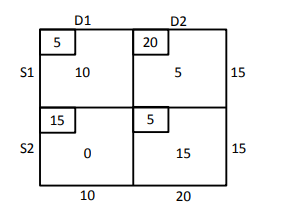
\includegraphics[width=0.75\columnwidth]{chapters/10/7/2/4/figs/fig.png}
 \end{center}
\caption{}
\label{fig:10/7/2/4Fig1}
\end{figure}
\fi

\item Find the position vector of the mid point of the vector joining the points $\vec{P}$(2, 3, 4)
and $\vec{Q}$(4, 1, –2).
\\
\solution
		\begin{enumerate}[label=\thesubsection.\arabic*,ref=\thesubsection.\theenumi]
\item Find the coordinates of the point which divides the join of $(-1,7) $ and $ (4,-3)$ in the ratio 2:3.
	\\
		\solution
	\input{chapters/10/7/2/1/section.tex}
\item Find the coordinates of the point $\vec{R}$ on the line segment joining the points $\vec{P}(-1,3)$ and $\vec{Q}(2,5)$ such that $PR=\frac{3}{5}PQ$.
\item Find the ratio in which the point $\vec{P}\brak{\frac{3}{4},\frac{5}{12}}$ divides the line segment joining the points $\vec{A}\brak{\frac{1}{2},\frac{3}{2}}$ and $ \vec{B}(2,-5)$.
\item Find the coordinates of the point which divides the line segment joining the points $(4,-3)$ and $(8,5)$ in the ratio $3:1$ internally.
\item Find the coordinates of the point $\vec{P}$ on $AD$ such that $AP : PD = 2 : 1$.
\item If the point $\vec{P} (2, 1)$ lies on the line segment joining points $\vec{A} (4, 2)$  and $ \vec{B} (8, 4)$,
then
\begin{enumerate}
	\item $AP =\frac{1}{3}{AB}$ 
\item ${AP}={PE}$
\item ${PB}=\frac{1}{3}{AB}$
\item${AP}=\frac{1}{2}{AB}$
 \end{enumerate}
\item Find the ratio in which the line segment joining the points $(-3,10)$  and  $(6,-8)$  is divided by $ (-1,6)$.
	\\
		\solution
	\input{chapters/10/7/2/4/section.tex}
\item Find the position vector of the mid point of the vector joining the points $\vec{P}$(2, 3, 4)
and $\vec{Q}$(4, 1, –2).
\\
\solution
		\input{chapters/12/10/2/16/section.tex}
\item Let $\vec{A}(4, 2), \vec{B}(6, 5)$  and $ \vec{C}(1, 4)$ be the vertices of $\triangle ABC$.
\begin{enumerate}
\item If $\vec{A}$ and  $\vec{B}$ are $(-2,-2)$ and  $(2,-4)$, respectively, find the coordinates of $\vec{P}$ such that $AP= \frac {3}{7}AB$  and $ \vec{P}$ lies on the line segment $AB$.
	\\
		\solution
	\input{chapters/10/7/2/8/section.tex}
\item Find the coordinates of the points which divide the line segment joining $A(-2,2)$  and  $\vec{B}(2,8)$ into four equal parts.
	\\
		\solution
	\input{chapters/10/7/2/9/section.tex}
\item In what ratio does the point $(-4,6)$ divide the line segment joining the points $\vec{A}(-6,0)$ and $\vec{B}(3,-8)$?
\item Given that $\vec{P}(3,2,-4), \vec{Q}(5,4,-6)$ and $\vec{R}(9,8,-10)$ are collinear. Find the ratio in which $\vec{Q}$ divides $PR$.
\item Points $\vec{A}(-6,10),\vec{B}(-4,6)$  and  $\vec{C}(3,-8)$ are collinear such that $AB=  \frac{2}{9}AC$.
\item The point which divides the line segment joining the points $\vec{P} (7, –6) $  and  $\vec{Q}(3, 4)$ in the 
ratio 1 : 2 internally lies in  which quadrant?
\item Find the coordinates of the points of trisection of the line segment joining $(4,-1)$  and  $(-2,3)$.
	\\
		\solution
	\input{chapters/10/7/2/2/section.tex}
\item Find the coordinates of the points which trisect the line segment joining the points $\vec{P}(4,2,-6)$ and $\vec{Q}(10,-16,6)$.
\item Find the coordinates of the points of trisection (i.e. points dividing to three equal parts) of the line segment joining the points $\vec{A}(2,-2)$ and $\vec{B}(-7,4)$.
\item Point $\vec{P}(5,-3)$ is one of the two points of trisection of line segment joining the points $\vec{A}(7,-2)$ and $\vec{B}(1,-5)$
\item Find the position vector of a point $\vec{R}$ which divides the line joining two points $\vec{P}$
and $\vec{Q}$ whose position vectors are $\hat{i}+2\hat{j}-\hat{k}$ and $-\hat{i}+\hat{j}+\hat{k}$ respectively, in the
ratio 2 : 1
\begin{enumerate}
    \item  internally
    \item  externally
\end{enumerate}
%\solution
%		\input{chapters/12/10/2/15/section.tex}
\item Find the coordinates of the point which divides the line segment joining the points which divides the line segment joining  the points $(-2,3,5)$ and $(1,-4,6)$ in the ratio 
\begin{enumerate}
\item $2:3$ internally,
\item $2:3$ externally
\end{enumerate}
\item Find the coordinates of the point which divides the line segment joining the points $(1,-2,3)$ and $(3,4,-5)$ in the ratio $2:3$
\begin{enumerate}
\item internally, and
\item externally
\end{enumerate}
\item Consider two points $\vec{P}$ and $\vec{Q}$ with position vectors $\overrightarrow{OP} = 3\overrightarrow{a}-2\overrightarrow{b}$ and $\overrightarrow{OQ}=\overrightarrow{a}+\overrightarrow{b}$. Find the position vector of a point $\vec{R}$ which divides the line joining $\vec{P}$ and $\vec{Q}$ in the ratio $2:1$, 
\begin{enumerate}
\item internally, and 
\item externally.
\end{enumerate}
\item The median from $\vec{A}$ meets $BC$ at $\vec{D}$. Find the coordinates of the point $\vec{D}$.
\item Find the coordinates of points $\vec{Q}$ and $\vec{R}$ on medians $BE$ and $CF$ respectively such that $BQ : QE = 2 : 1$  and  $CR : RF = 2 : 1$.
\item What do you observe?
\item If $\vec{A}, \vec{B}$ and $\vec{C}$  are the vertices of $\triangle ABC$, find the coordinates of the centroid of the triangle.
\end{enumerate}
\solution
	\input{chapters/10/7/4/7/section.tex}
\item If $\vec{P}(9a-2,-b)$ divides line segment joining $\vec{A}(3a+1,-3)$ and $\vec{B}(8a,5)$ in the ratio 3:1, find the values of $a$ and $b$.
\item Find the position vector of a point $\vec{R}$ which divides the line joining two points $\vec{P}$ and $\vec{Q}$ whose position vectors are $2\vec{a}+\vec{b}$ and $\vec{a}-3\vec{b}$ externally in the ratio $1:2$.
\item The position vector of the point which divides the join of points 2$\vec{a}$-3$\vec{b}$ $\text{and}$ $\vec{a}+\vec{b}$ in the ratio 3:1 is \rule{1cm}{0.1pt}.
\item If $\vec{a}$ and $\vec{b}$ are the postion vectors of $\vec{A}$ and $\vec{B}$, respectively, find the position vector of a point $\vec{C}$ in $BA$ produced such that $BC=1.5BA$.
\item Find the position vector of a point $\vec{R}$ which divides the line joining two points $\vec{P}$ and $\vec{Q}$ whose position vectors are $(2\vec{a}+\vec{b})$ and $(\vec{a}-3\vec{b})$
externally in the ratio 1 : 2. Also, show that $\vec{P}$ is the mid point of the line segment $RQ$.
\end{enumerate}

\item Let $\vec{A}(4, 2), \vec{B}(6, 5)$  and $ \vec{C}(1, 4)$ be the vertices of $\triangle ABC$.
\begin{enumerate}
\item If $\vec{A}$ and  $\vec{B}$ are $(-2,-2)$ and  $(2,-4)$, respectively, find the coordinates of $\vec{P}$ such that $AP= \frac {3}{7}AB$  and $ \vec{P}$ lies on the line segment $AB$.
	\\
		\solution
	\begin{enumerate}[label=\thesubsection.\arabic*,ref=\thesubsection.\theenumi]
\item Find the coordinates of the point which divides the join of $(-1,7) $ and $ (4,-3)$ in the ratio 2:3.
	\\
		\solution
	\input{chapters/10/7/2/1/section.tex}
\item Find the coordinates of the point $\vec{R}$ on the line segment joining the points $\vec{P}(-1,3)$ and $\vec{Q}(2,5)$ such that $PR=\frac{3}{5}PQ$.
\item Find the ratio in which the point $\vec{P}\brak{\frac{3}{4},\frac{5}{12}}$ divides the line segment joining the points $\vec{A}\brak{\frac{1}{2},\frac{3}{2}}$ and $ \vec{B}(2,-5)$.
\item Find the coordinates of the point which divides the line segment joining the points $(4,-3)$ and $(8,5)$ in the ratio $3:1$ internally.
\item Find the coordinates of the point $\vec{P}$ on $AD$ such that $AP : PD = 2 : 1$.
\item If the point $\vec{P} (2, 1)$ lies on the line segment joining points $\vec{A} (4, 2)$  and $ \vec{B} (8, 4)$,
then
\begin{enumerate}
	\item $AP =\frac{1}{3}{AB}$ 
\item ${AP}={PE}$
\item ${PB}=\frac{1}{3}{AB}$
\item${AP}=\frac{1}{2}{AB}$
 \end{enumerate}
\item Find the ratio in which the line segment joining the points $(-3,10)$  and  $(6,-8)$  is divided by $ (-1,6)$.
	\\
		\solution
	\input{chapters/10/7/2/4/section.tex}
\item Find the position vector of the mid point of the vector joining the points $\vec{P}$(2, 3, 4)
and $\vec{Q}$(4, 1, –2).
\\
\solution
		\input{chapters/12/10/2/16/section.tex}
\item Let $\vec{A}(4, 2), \vec{B}(6, 5)$  and $ \vec{C}(1, 4)$ be the vertices of $\triangle ABC$.
\begin{enumerate}
\item If $\vec{A}$ and  $\vec{B}$ are $(-2,-2)$ and  $(2,-4)$, respectively, find the coordinates of $\vec{P}$ such that $AP= \frac {3}{7}AB$  and $ \vec{P}$ lies on the line segment $AB$.
	\\
		\solution
	\input{chapters/10/7/2/8/section.tex}
\item Find the coordinates of the points which divide the line segment joining $A(-2,2)$  and  $\vec{B}(2,8)$ into four equal parts.
	\\
		\solution
	\input{chapters/10/7/2/9/section.tex}
\item In what ratio does the point $(-4,6)$ divide the line segment joining the points $\vec{A}(-6,0)$ and $\vec{B}(3,-8)$?
\item Given that $\vec{P}(3,2,-4), \vec{Q}(5,4,-6)$ and $\vec{R}(9,8,-10)$ are collinear. Find the ratio in which $\vec{Q}$ divides $PR$.
\item Points $\vec{A}(-6,10),\vec{B}(-4,6)$  and  $\vec{C}(3,-8)$ are collinear such that $AB=  \frac{2}{9}AC$.
\item The point which divides the line segment joining the points $\vec{P} (7, –6) $  and  $\vec{Q}(3, 4)$ in the 
ratio 1 : 2 internally lies in  which quadrant?
\item Find the coordinates of the points of trisection of the line segment joining $(4,-1)$  and  $(-2,3)$.
	\\
		\solution
	\input{chapters/10/7/2/2/section.tex}
\item Find the coordinates of the points which trisect the line segment joining the points $\vec{P}(4,2,-6)$ and $\vec{Q}(10,-16,6)$.
\item Find the coordinates of the points of trisection (i.e. points dividing to three equal parts) of the line segment joining the points $\vec{A}(2,-2)$ and $\vec{B}(-7,4)$.
\item Point $\vec{P}(5,-3)$ is one of the two points of trisection of line segment joining the points $\vec{A}(7,-2)$ and $\vec{B}(1,-5)$
\item Find the position vector of a point $\vec{R}$ which divides the line joining two points $\vec{P}$
and $\vec{Q}$ whose position vectors are $\hat{i}+2\hat{j}-\hat{k}$ and $-\hat{i}+\hat{j}+\hat{k}$ respectively, in the
ratio 2 : 1
\begin{enumerate}
    \item  internally
    \item  externally
\end{enumerate}
%\solution
%		\input{chapters/12/10/2/15/section.tex}
\item Find the coordinates of the point which divides the line segment joining the points which divides the line segment joining  the points $(-2,3,5)$ and $(1,-4,6)$ in the ratio 
\begin{enumerate}
\item $2:3$ internally,
\item $2:3$ externally
\end{enumerate}
\item Find the coordinates of the point which divides the line segment joining the points $(1,-2,3)$ and $(3,4,-5)$ in the ratio $2:3$
\begin{enumerate}
\item internally, and
\item externally
\end{enumerate}
\item Consider two points $\vec{P}$ and $\vec{Q}$ with position vectors $\overrightarrow{OP} = 3\overrightarrow{a}-2\overrightarrow{b}$ and $\overrightarrow{OQ}=\overrightarrow{a}+\overrightarrow{b}$. Find the position vector of a point $\vec{R}$ which divides the line joining $\vec{P}$ and $\vec{Q}$ in the ratio $2:1$, 
\begin{enumerate}
\item internally, and 
\item externally.
\end{enumerate}
\item The median from $\vec{A}$ meets $BC$ at $\vec{D}$. Find the coordinates of the point $\vec{D}$.
\item Find the coordinates of points $\vec{Q}$ and $\vec{R}$ on medians $BE$ and $CF$ respectively such that $BQ : QE = 2 : 1$  and  $CR : RF = 2 : 1$.
\item What do you observe?
\item If $\vec{A}, \vec{B}$ and $\vec{C}$  are the vertices of $\triangle ABC$, find the coordinates of the centroid of the triangle.
\end{enumerate}
\solution
	\input{chapters/10/7/4/7/section.tex}
\item If $\vec{P}(9a-2,-b)$ divides line segment joining $\vec{A}(3a+1,-3)$ and $\vec{B}(8a,5)$ in the ratio 3:1, find the values of $a$ and $b$.
\item Find the position vector of a point $\vec{R}$ which divides the line joining two points $\vec{P}$ and $\vec{Q}$ whose position vectors are $2\vec{a}+\vec{b}$ and $\vec{a}-3\vec{b}$ externally in the ratio $1:2$.
\item The position vector of the point which divides the join of points 2$\vec{a}$-3$\vec{b}$ $\text{and}$ $\vec{a}+\vec{b}$ in the ratio 3:1 is \rule{1cm}{0.1pt}.
\item If $\vec{a}$ and $\vec{b}$ are the postion vectors of $\vec{A}$ and $\vec{B}$, respectively, find the position vector of a point $\vec{C}$ in $BA$ produced such that $BC=1.5BA$.
\item Find the position vector of a point $\vec{R}$ which divides the line joining two points $\vec{P}$ and $\vec{Q}$ whose position vectors are $(2\vec{a}+\vec{b})$ and $(\vec{a}-3\vec{b})$
externally in the ratio 1 : 2. Also, show that $\vec{P}$ is the mid point of the line segment $RQ$.
\end{enumerate}

\item Find the coordinates of the points which divide the line segment joining $A(-2,2)$  and  $\vec{B}(2,8)$ into four equal parts.
	\\
		\solution
	\begin{enumerate}[label=\thesubsection.\arabic*,ref=\thesubsection.\theenumi]
\item Find the coordinates of the point which divides the join of $(-1,7) $ and $ (4,-3)$ in the ratio 2:3.
	\\
		\solution
	\input{chapters/10/7/2/1/section.tex}
\item Find the coordinates of the point $\vec{R}$ on the line segment joining the points $\vec{P}(-1,3)$ and $\vec{Q}(2,5)$ such that $PR=\frac{3}{5}PQ$.
\item Find the ratio in which the point $\vec{P}\brak{\frac{3}{4},\frac{5}{12}}$ divides the line segment joining the points $\vec{A}\brak{\frac{1}{2},\frac{3}{2}}$ and $ \vec{B}(2,-5)$.
\item Find the coordinates of the point which divides the line segment joining the points $(4,-3)$ and $(8,5)$ in the ratio $3:1$ internally.
\item Find the coordinates of the point $\vec{P}$ on $AD$ such that $AP : PD = 2 : 1$.
\item If the point $\vec{P} (2, 1)$ lies on the line segment joining points $\vec{A} (4, 2)$  and $ \vec{B} (8, 4)$,
then
\begin{enumerate}
	\item $AP =\frac{1}{3}{AB}$ 
\item ${AP}={PE}$
\item ${PB}=\frac{1}{3}{AB}$
\item${AP}=\frac{1}{2}{AB}$
 \end{enumerate}
\item Find the ratio in which the line segment joining the points $(-3,10)$  and  $(6,-8)$  is divided by $ (-1,6)$.
	\\
		\solution
	\input{chapters/10/7/2/4/section.tex}
\item Find the position vector of the mid point of the vector joining the points $\vec{P}$(2, 3, 4)
and $\vec{Q}$(4, 1, –2).
\\
\solution
		\input{chapters/12/10/2/16/section.tex}
\item Let $\vec{A}(4, 2), \vec{B}(6, 5)$  and $ \vec{C}(1, 4)$ be the vertices of $\triangle ABC$.
\begin{enumerate}
\item If $\vec{A}$ and  $\vec{B}$ are $(-2,-2)$ and  $(2,-4)$, respectively, find the coordinates of $\vec{P}$ such that $AP= \frac {3}{7}AB$  and $ \vec{P}$ lies on the line segment $AB$.
	\\
		\solution
	\input{chapters/10/7/2/8/section.tex}
\item Find the coordinates of the points which divide the line segment joining $A(-2,2)$  and  $\vec{B}(2,8)$ into four equal parts.
	\\
		\solution
	\input{chapters/10/7/2/9/section.tex}
\item In what ratio does the point $(-4,6)$ divide the line segment joining the points $\vec{A}(-6,0)$ and $\vec{B}(3,-8)$?
\item Given that $\vec{P}(3,2,-4), \vec{Q}(5,4,-6)$ and $\vec{R}(9,8,-10)$ are collinear. Find the ratio in which $\vec{Q}$ divides $PR$.
\item Points $\vec{A}(-6,10),\vec{B}(-4,6)$  and  $\vec{C}(3,-8)$ are collinear such that $AB=  \frac{2}{9}AC$.
\item The point which divides the line segment joining the points $\vec{P} (7, –6) $  and  $\vec{Q}(3, 4)$ in the 
ratio 1 : 2 internally lies in  which quadrant?
\item Find the coordinates of the points of trisection of the line segment joining $(4,-1)$  and  $(-2,3)$.
	\\
		\solution
	\input{chapters/10/7/2/2/section.tex}
\item Find the coordinates of the points which trisect the line segment joining the points $\vec{P}(4,2,-6)$ and $\vec{Q}(10,-16,6)$.
\item Find the coordinates of the points of trisection (i.e. points dividing to three equal parts) of the line segment joining the points $\vec{A}(2,-2)$ and $\vec{B}(-7,4)$.
\item Point $\vec{P}(5,-3)$ is one of the two points of trisection of line segment joining the points $\vec{A}(7,-2)$ and $\vec{B}(1,-5)$
\item Find the position vector of a point $\vec{R}$ which divides the line joining two points $\vec{P}$
and $\vec{Q}$ whose position vectors are $\hat{i}+2\hat{j}-\hat{k}$ and $-\hat{i}+\hat{j}+\hat{k}$ respectively, in the
ratio 2 : 1
\begin{enumerate}
    \item  internally
    \item  externally
\end{enumerate}
%\solution
%		\input{chapters/12/10/2/15/section.tex}
\item Find the coordinates of the point which divides the line segment joining the points which divides the line segment joining  the points $(-2,3,5)$ and $(1,-4,6)$ in the ratio 
\begin{enumerate}
\item $2:3$ internally,
\item $2:3$ externally
\end{enumerate}
\item Find the coordinates of the point which divides the line segment joining the points $(1,-2,3)$ and $(3,4,-5)$ in the ratio $2:3$
\begin{enumerate}
\item internally, and
\item externally
\end{enumerate}
\item Consider two points $\vec{P}$ and $\vec{Q}$ with position vectors $\overrightarrow{OP} = 3\overrightarrow{a}-2\overrightarrow{b}$ and $\overrightarrow{OQ}=\overrightarrow{a}+\overrightarrow{b}$. Find the position vector of a point $\vec{R}$ which divides the line joining $\vec{P}$ and $\vec{Q}$ in the ratio $2:1$, 
\begin{enumerate}
\item internally, and 
\item externally.
\end{enumerate}
\item The median from $\vec{A}$ meets $BC$ at $\vec{D}$. Find the coordinates of the point $\vec{D}$.
\item Find the coordinates of points $\vec{Q}$ and $\vec{R}$ on medians $BE$ and $CF$ respectively such that $BQ : QE = 2 : 1$  and  $CR : RF = 2 : 1$.
\item What do you observe?
\item If $\vec{A}, \vec{B}$ and $\vec{C}$  are the vertices of $\triangle ABC$, find the coordinates of the centroid of the triangle.
\end{enumerate}
\solution
	\input{chapters/10/7/4/7/section.tex}
\item If $\vec{P}(9a-2,-b)$ divides line segment joining $\vec{A}(3a+1,-3)$ and $\vec{B}(8a,5)$ in the ratio 3:1, find the values of $a$ and $b$.
\item Find the position vector of a point $\vec{R}$ which divides the line joining two points $\vec{P}$ and $\vec{Q}$ whose position vectors are $2\vec{a}+\vec{b}$ and $\vec{a}-3\vec{b}$ externally in the ratio $1:2$.
\item The position vector of the point which divides the join of points 2$\vec{a}$-3$\vec{b}$ $\text{and}$ $\vec{a}+\vec{b}$ in the ratio 3:1 is \rule{1cm}{0.1pt}.
\item If $\vec{a}$ and $\vec{b}$ are the postion vectors of $\vec{A}$ and $\vec{B}$, respectively, find the position vector of a point $\vec{C}$ in $BA$ produced such that $BC=1.5BA$.
\item Find the position vector of a point $\vec{R}$ which divides the line joining two points $\vec{P}$ and $\vec{Q}$ whose position vectors are $(2\vec{a}+\vec{b})$ and $(\vec{a}-3\vec{b})$
externally in the ratio 1 : 2. Also, show that $\vec{P}$ is the mid point of the line segment $RQ$.
\end{enumerate}

\item In what ratio does the point $(-4,6)$ divide the line segment joining the points $\vec{A}(-6,0)$ and $\vec{B}(3,-8)$?
\item Given that $\vec{P}(3,2,-4), \vec{Q}(5,4,-6)$ and $\vec{R}(9,8,-10)$ are collinear. Find the ratio in which $\vec{Q}$ divides $PR$.
\item Points $\vec{A}(-6,10),\vec{B}(-4,6)$  and  $\vec{C}(3,-8)$ are collinear such that $AB=  \frac{2}{9}AC$.
\item The point which divides the line segment joining the points $\vec{P} (7, –6) $  and  $\vec{Q}(3, 4)$ in the 
ratio 1 : 2 internally lies in  which quadrant?
\item Find the coordinates of the points of trisection of the line segment joining $(4,-1)$  and  $(-2,3)$.
	\\
		\solution
	Using section formula,
\begin{align}
\vec{R}=\frac{1}{1+\frac{1}{2}}\brak{\myvec{4\\-1}+\frac{1}{2}\myvec{-2\\3}}
=\myvec{2\\ \frac{1}{3}}\\
\vec{S}=\frac{1}{1+\frac{2}{1}}\brak{\myvec{4\\-1}+\frac{2}{1}\myvec{-2\\3}}
=\myvec{0\\ \frac{5}{3}}
\end{align}
which are the desired points of trisection.
\iffalse
See
		\figref{fig:chapters/10/7/2/2/Figure}
\begin{figure}[H]
\centering
\includegraphics[width=0.75\columnwidth]{chapters/10/7/2/2/figs/dj.pdf}
\caption{}
		\label{fig:chapters/10/7/2/2/Figure}
\end{figure}
\fi

\item Find the coordinates of the points which trisect the line segment joining the points $\vec{P}(4,2,-6)$ and $\vec{Q}(10,-16,6)$.
\item Find the coordinates of the points of trisection (i.e. points dividing to three equal parts) of the line segment joining the points $\vec{A}(2,-2)$ and $\vec{B}(-7,4)$.
\item Point $\vec{P}(5,-3)$ is one of the two points of trisection of line segment joining the points $\vec{A}(7,-2)$ and $\vec{B}(1,-5)$
\item Find the position vector of a point $\vec{R}$ which divides the line joining two points $\vec{P}$
and $\vec{Q}$ whose position vectors are $\hat{i}+2\hat{j}-\hat{k}$ and $-\hat{i}+\hat{j}+\hat{k}$ respectively, in the
ratio 2 : 1
\begin{enumerate}
    \item  internally
    \item  externally
\end{enumerate}
%\solution
%		\begin{enumerate}[label=\thesubsection.\arabic*,ref=\thesubsection.\theenumi]
\item Find the coordinates of the point which divides the join of $(-1,7) $ and $ (4,-3)$ in the ratio 2:3.
	\\
		\solution
	\input{chapters/10/7/2/1/section.tex}
\item Find the coordinates of the point $\vec{R}$ on the line segment joining the points $\vec{P}(-1,3)$ and $\vec{Q}(2,5)$ such that $PR=\frac{3}{5}PQ$.
\item Find the ratio in which the point $\vec{P}\brak{\frac{3}{4},\frac{5}{12}}$ divides the line segment joining the points $\vec{A}\brak{\frac{1}{2},\frac{3}{2}}$ and $ \vec{B}(2,-5)$.
\item Find the coordinates of the point which divides the line segment joining the points $(4,-3)$ and $(8,5)$ in the ratio $3:1$ internally.
\item Find the coordinates of the point $\vec{P}$ on $AD$ such that $AP : PD = 2 : 1$.
\item If the point $\vec{P} (2, 1)$ lies on the line segment joining points $\vec{A} (4, 2)$  and $ \vec{B} (8, 4)$,
then
\begin{enumerate}
	\item $AP =\frac{1}{3}{AB}$ 
\item ${AP}={PE}$
\item ${PB}=\frac{1}{3}{AB}$
\item${AP}=\frac{1}{2}{AB}$
 \end{enumerate}
\item Find the ratio in which the line segment joining the points $(-3,10)$  and  $(6,-8)$  is divided by $ (-1,6)$.
	\\
		\solution
	\input{chapters/10/7/2/4/section.tex}
\item Find the position vector of the mid point of the vector joining the points $\vec{P}$(2, 3, 4)
and $\vec{Q}$(4, 1, –2).
\\
\solution
		\input{chapters/12/10/2/16/section.tex}
\item Let $\vec{A}(4, 2), \vec{B}(6, 5)$  and $ \vec{C}(1, 4)$ be the vertices of $\triangle ABC$.
\begin{enumerate}
\item If $\vec{A}$ and  $\vec{B}$ are $(-2,-2)$ and  $(2,-4)$, respectively, find the coordinates of $\vec{P}$ such that $AP= \frac {3}{7}AB$  and $ \vec{P}$ lies on the line segment $AB$.
	\\
		\solution
	\input{chapters/10/7/2/8/section.tex}
\item Find the coordinates of the points which divide the line segment joining $A(-2,2)$  and  $\vec{B}(2,8)$ into four equal parts.
	\\
		\solution
	\input{chapters/10/7/2/9/section.tex}
\item In what ratio does the point $(-4,6)$ divide the line segment joining the points $\vec{A}(-6,0)$ and $\vec{B}(3,-8)$?
\item Given that $\vec{P}(3,2,-4), \vec{Q}(5,4,-6)$ and $\vec{R}(9,8,-10)$ are collinear. Find the ratio in which $\vec{Q}$ divides $PR$.
\item Points $\vec{A}(-6,10),\vec{B}(-4,6)$  and  $\vec{C}(3,-8)$ are collinear such that $AB=  \frac{2}{9}AC$.
\item The point which divides the line segment joining the points $\vec{P} (7, –6) $  and  $\vec{Q}(3, 4)$ in the 
ratio 1 : 2 internally lies in  which quadrant?
\item Find the coordinates of the points of trisection of the line segment joining $(4,-1)$  and  $(-2,3)$.
	\\
		\solution
	\input{chapters/10/7/2/2/section.tex}
\item Find the coordinates of the points which trisect the line segment joining the points $\vec{P}(4,2,-6)$ and $\vec{Q}(10,-16,6)$.
\item Find the coordinates of the points of trisection (i.e. points dividing to three equal parts) of the line segment joining the points $\vec{A}(2,-2)$ and $\vec{B}(-7,4)$.
\item Point $\vec{P}(5,-3)$ is one of the two points of trisection of line segment joining the points $\vec{A}(7,-2)$ and $\vec{B}(1,-5)$
\item Find the position vector of a point $\vec{R}$ which divides the line joining two points $\vec{P}$
and $\vec{Q}$ whose position vectors are $\hat{i}+2\hat{j}-\hat{k}$ and $-\hat{i}+\hat{j}+\hat{k}$ respectively, in the
ratio 2 : 1
\begin{enumerate}
    \item  internally
    \item  externally
\end{enumerate}
%\solution
%		\input{chapters/12/10/2/15/section.tex}
\item Find the coordinates of the point which divides the line segment joining the points which divides the line segment joining  the points $(-2,3,5)$ and $(1,-4,6)$ in the ratio 
\begin{enumerate}
\item $2:3$ internally,
\item $2:3$ externally
\end{enumerate}
\item Find the coordinates of the point which divides the line segment joining the points $(1,-2,3)$ and $(3,4,-5)$ in the ratio $2:3$
\begin{enumerate}
\item internally, and
\item externally
\end{enumerate}
\item Consider two points $\vec{P}$ and $\vec{Q}$ with position vectors $\overrightarrow{OP} = 3\overrightarrow{a}-2\overrightarrow{b}$ and $\overrightarrow{OQ}=\overrightarrow{a}+\overrightarrow{b}$. Find the position vector of a point $\vec{R}$ which divides the line joining $\vec{P}$ and $\vec{Q}$ in the ratio $2:1$, 
\begin{enumerate}
\item internally, and 
\item externally.
\end{enumerate}
\item The median from $\vec{A}$ meets $BC$ at $\vec{D}$. Find the coordinates of the point $\vec{D}$.
\item Find the coordinates of points $\vec{Q}$ and $\vec{R}$ on medians $BE$ and $CF$ respectively such that $BQ : QE = 2 : 1$  and  $CR : RF = 2 : 1$.
\item What do you observe?
\item If $\vec{A}, \vec{B}$ and $\vec{C}$  are the vertices of $\triangle ABC$, find the coordinates of the centroid of the triangle.
\end{enumerate}
\solution
	\input{chapters/10/7/4/7/section.tex}
\item If $\vec{P}(9a-2,-b)$ divides line segment joining $\vec{A}(3a+1,-3)$ and $\vec{B}(8a,5)$ in the ratio 3:1, find the values of $a$ and $b$.
\item Find the position vector of a point $\vec{R}$ which divides the line joining two points $\vec{P}$ and $\vec{Q}$ whose position vectors are $2\vec{a}+\vec{b}$ and $\vec{a}-3\vec{b}$ externally in the ratio $1:2$.
\item The position vector of the point which divides the join of points 2$\vec{a}$-3$\vec{b}$ $\text{and}$ $\vec{a}+\vec{b}$ in the ratio 3:1 is \rule{1cm}{0.1pt}.
\item If $\vec{a}$ and $\vec{b}$ are the postion vectors of $\vec{A}$ and $\vec{B}$, respectively, find the position vector of a point $\vec{C}$ in $BA$ produced such that $BC=1.5BA$.
\item Find the position vector of a point $\vec{R}$ which divides the line joining two points $\vec{P}$ and $\vec{Q}$ whose position vectors are $(2\vec{a}+\vec{b})$ and $(\vec{a}-3\vec{b})$
externally in the ratio 1 : 2. Also, show that $\vec{P}$ is the mid point of the line segment $RQ$.
\end{enumerate}

\item Find the coordinates of the point which divides the line segment joining the points which divides the line segment joining  the points $(-2,3,5)$ and $(1,-4,6)$ in the ratio 
\begin{enumerate}
\item $2:3$ internally,
\item $2:3$ externally
\end{enumerate}
\item Find the coordinates of the point which divides the line segment joining the points $(1,-2,3)$ and $(3,4,-5)$ in the ratio $2:3$
\begin{enumerate}
\item internally, and
\item externally
\end{enumerate}
\item Consider two points $\vec{P}$ and $\vec{Q}$ with position vectors $\overrightarrow{OP} = 3\overrightarrow{a}-2\overrightarrow{b}$ and $\overrightarrow{OQ}=\overrightarrow{a}+\overrightarrow{b}$. Find the position vector of a point $\vec{R}$ which divides the line joining $\vec{P}$ and $\vec{Q}$ in the ratio $2:1$, 
\begin{enumerate}
\item internally, and 
\item externally.
\end{enumerate}
\item The median from $\vec{A}$ meets $BC$ at $\vec{D}$. Find the coordinates of the point $\vec{D}$.
\item Find the coordinates of points $\vec{Q}$ and $\vec{R}$ on medians $BE$ and $CF$ respectively such that $BQ : QE = 2 : 1$  and  $CR : RF = 2 : 1$.
\item What do you observe?
\item If $\vec{A}, \vec{B}$ and $\vec{C}$  are the vertices of $\triangle ABC$, find the coordinates of the centroid of the triangle.
\end{enumerate}
\solution
	\begin{enumerate}[label=\thesubsection.\arabic*,ref=\thesubsection.\theenumi]
\item Find the coordinates of the point which divides the join of $(-1,7) $ and $ (4,-3)$ in the ratio 2:3.
	\\
		\solution
	\input{chapters/10/7/2/1/section.tex}
\item Find the coordinates of the point $\vec{R}$ on the line segment joining the points $\vec{P}(-1,3)$ and $\vec{Q}(2,5)$ such that $PR=\frac{3}{5}PQ$.
\item Find the ratio in which the point $\vec{P}\brak{\frac{3}{4},\frac{5}{12}}$ divides the line segment joining the points $\vec{A}\brak{\frac{1}{2},\frac{3}{2}}$ and $ \vec{B}(2,-5)$.
\item Find the coordinates of the point which divides the line segment joining the points $(4,-3)$ and $(8,5)$ in the ratio $3:1$ internally.
\item Find the coordinates of the point $\vec{P}$ on $AD$ such that $AP : PD = 2 : 1$.
\item If the point $\vec{P} (2, 1)$ lies on the line segment joining points $\vec{A} (4, 2)$  and $ \vec{B} (8, 4)$,
then
\begin{enumerate}
	\item $AP =\frac{1}{3}{AB}$ 
\item ${AP}={PE}$
\item ${PB}=\frac{1}{3}{AB}$
\item${AP}=\frac{1}{2}{AB}$
 \end{enumerate}
\item Find the ratio in which the line segment joining the points $(-3,10)$  and  $(6,-8)$  is divided by $ (-1,6)$.
	\\
		\solution
	\input{chapters/10/7/2/4/section.tex}
\item Find the position vector of the mid point of the vector joining the points $\vec{P}$(2, 3, 4)
and $\vec{Q}$(4, 1, –2).
\\
\solution
		\input{chapters/12/10/2/16/section.tex}
\item Let $\vec{A}(4, 2), \vec{B}(6, 5)$  and $ \vec{C}(1, 4)$ be the vertices of $\triangle ABC$.
\begin{enumerate}
\item If $\vec{A}$ and  $\vec{B}$ are $(-2,-2)$ and  $(2,-4)$, respectively, find the coordinates of $\vec{P}$ such that $AP= \frac {3}{7}AB$  and $ \vec{P}$ lies on the line segment $AB$.
	\\
		\solution
	\input{chapters/10/7/2/8/section.tex}
\item Find the coordinates of the points which divide the line segment joining $A(-2,2)$  and  $\vec{B}(2,8)$ into four equal parts.
	\\
		\solution
	\input{chapters/10/7/2/9/section.tex}
\item In what ratio does the point $(-4,6)$ divide the line segment joining the points $\vec{A}(-6,0)$ and $\vec{B}(3,-8)$?
\item Given that $\vec{P}(3,2,-4), \vec{Q}(5,4,-6)$ and $\vec{R}(9,8,-10)$ are collinear. Find the ratio in which $\vec{Q}$ divides $PR$.
\item Points $\vec{A}(-6,10),\vec{B}(-4,6)$  and  $\vec{C}(3,-8)$ are collinear such that $AB=  \frac{2}{9}AC$.
\item The point which divides the line segment joining the points $\vec{P} (7, –6) $  and  $\vec{Q}(3, 4)$ in the 
ratio 1 : 2 internally lies in  which quadrant?
\item Find the coordinates of the points of trisection of the line segment joining $(4,-1)$  and  $(-2,3)$.
	\\
		\solution
	\input{chapters/10/7/2/2/section.tex}
\item Find the coordinates of the points which trisect the line segment joining the points $\vec{P}(4,2,-6)$ and $\vec{Q}(10,-16,6)$.
\item Find the coordinates of the points of trisection (i.e. points dividing to three equal parts) of the line segment joining the points $\vec{A}(2,-2)$ and $\vec{B}(-7,4)$.
\item Point $\vec{P}(5,-3)$ is one of the two points of trisection of line segment joining the points $\vec{A}(7,-2)$ and $\vec{B}(1,-5)$
\item Find the position vector of a point $\vec{R}$ which divides the line joining two points $\vec{P}$
and $\vec{Q}$ whose position vectors are $\hat{i}+2\hat{j}-\hat{k}$ and $-\hat{i}+\hat{j}+\hat{k}$ respectively, in the
ratio 2 : 1
\begin{enumerate}
    \item  internally
    \item  externally
\end{enumerate}
%\solution
%		\input{chapters/12/10/2/15/section.tex}
\item Find the coordinates of the point which divides the line segment joining the points which divides the line segment joining  the points $(-2,3,5)$ and $(1,-4,6)$ in the ratio 
\begin{enumerate}
\item $2:3$ internally,
\item $2:3$ externally
\end{enumerate}
\item Find the coordinates of the point which divides the line segment joining the points $(1,-2,3)$ and $(3,4,-5)$ in the ratio $2:3$
\begin{enumerate}
\item internally, and
\item externally
\end{enumerate}
\item Consider two points $\vec{P}$ and $\vec{Q}$ with position vectors $\overrightarrow{OP} = 3\overrightarrow{a}-2\overrightarrow{b}$ and $\overrightarrow{OQ}=\overrightarrow{a}+\overrightarrow{b}$. Find the position vector of a point $\vec{R}$ which divides the line joining $\vec{P}$ and $\vec{Q}$ in the ratio $2:1$, 
\begin{enumerate}
\item internally, and 
\item externally.
\end{enumerate}
\item The median from $\vec{A}$ meets $BC$ at $\vec{D}$. Find the coordinates of the point $\vec{D}$.
\item Find the coordinates of points $\vec{Q}$ and $\vec{R}$ on medians $BE$ and $CF$ respectively such that $BQ : QE = 2 : 1$  and  $CR : RF = 2 : 1$.
\item What do you observe?
\item If $\vec{A}, \vec{B}$ and $\vec{C}$  are the vertices of $\triangle ABC$, find the coordinates of the centroid of the triangle.
\end{enumerate}
\solution
	\input{chapters/10/7/4/7/section.tex}
\item If $\vec{P}(9a-2,-b)$ divides line segment joining $\vec{A}(3a+1,-3)$ and $\vec{B}(8a,5)$ in the ratio 3:1, find the values of $a$ and $b$.
\item Find the position vector of a point $\vec{R}$ which divides the line joining two points $\vec{P}$ and $\vec{Q}$ whose position vectors are $2\vec{a}+\vec{b}$ and $\vec{a}-3\vec{b}$ externally in the ratio $1:2$.
\item The position vector of the point which divides the join of points 2$\vec{a}$-3$\vec{b}$ $\text{and}$ $\vec{a}+\vec{b}$ in the ratio 3:1 is \rule{1cm}{0.1pt}.
\item If $\vec{a}$ and $\vec{b}$ are the postion vectors of $\vec{A}$ and $\vec{B}$, respectively, find the position vector of a point $\vec{C}$ in $BA$ produced such that $BC=1.5BA$.
\item Find the position vector of a point $\vec{R}$ which divides the line joining two points $\vec{P}$ and $\vec{Q}$ whose position vectors are $(2\vec{a}+\vec{b})$ and $(\vec{a}-3\vec{b})$
externally in the ratio 1 : 2. Also, show that $\vec{P}$ is the mid point of the line segment $RQ$.
\end{enumerate}

\item If $\vec{P}(9a-2,-b)$ divides line segment joining $\vec{A}(3a+1,-3)$ and $\vec{B}(8a,5)$ in the ratio 3:1, find the values of $a$ and $b$.
\item Find the position vector of a point $\vec{R}$ which divides the line joining two points $\vec{P}$ and $\vec{Q}$ whose position vectors are $2\vec{a}+\vec{b}$ and $\vec{a}-3\vec{b}$ externally in the ratio $1:2$.
\item The position vector of the point which divides the join of points 2$\vec{a}$-3$\vec{b}$ $\text{and}$ $\vec{a}+\vec{b}$ in the ratio 3:1 is \rule{1cm}{0.1pt}.
\item If $\vec{a}$ and $\vec{b}$ are the postion vectors of $\vec{A}$ and $\vec{B}$, respectively, find the position vector of a point $\vec{C}$ in $BA$ produced such that $BC=1.5BA$.
\item Find the position vector of a point $\vec{R}$ which divides the line joining two points $\vec{P}$ and $\vec{Q}$ whose position vectors are $(2\vec{a}+\vec{b})$ and $(\vec{a}-3\vec{b})$
externally in the ratio 1 : 2. Also, show that $\vec{P}$ is the mid point of the line segment $RQ$.
\end{enumerate}

\item Let $\vec{A}(4, 2), \vec{B}(6, 5)$  and $ \vec{C}(1, 4)$ be the vertices of $\triangle ABC$.
\begin{enumerate}
\item If $\vec{A}$ and  $\vec{B}$ are $(-2,-2)$ and  $(2,-4)$, respectively, find the coordinates of $\vec{P}$ such that $AP= \frac {3}{7}AB$  and $ \vec{P}$ lies on the line segment $AB$.
	\\
		\solution
	\begin{enumerate}[label=\thesubsection.\arabic*,ref=\thesubsection.\theenumi]
\item Find the coordinates of the point which divides the join of $(-1,7) $ and $ (4,-3)$ in the ratio 2:3.
	\\
		\solution
	\begin{enumerate}[label=\thesubsection.\arabic*,ref=\thesubsection.\theenumi]
\item Find the coordinates of the point which divides the join of $(-1,7) $ and $ (4,-3)$ in the ratio 2:3.
	\\
		\solution
	\input{chapters/10/7/2/1/section.tex}
\item Find the coordinates of the point $\vec{R}$ on the line segment joining the points $\vec{P}(-1,3)$ and $\vec{Q}(2,5)$ such that $PR=\frac{3}{5}PQ$.
\item Find the ratio in which the point $\vec{P}\brak{\frac{3}{4},\frac{5}{12}}$ divides the line segment joining the points $\vec{A}\brak{\frac{1}{2},\frac{3}{2}}$ and $ \vec{B}(2,-5)$.
\item Find the coordinates of the point which divides the line segment joining the points $(4,-3)$ and $(8,5)$ in the ratio $3:1$ internally.
\item Find the coordinates of the point $\vec{P}$ on $AD$ such that $AP : PD = 2 : 1$.
\item If the point $\vec{P} (2, 1)$ lies on the line segment joining points $\vec{A} (4, 2)$  and $ \vec{B} (8, 4)$,
then
\begin{enumerate}
	\item $AP =\frac{1}{3}{AB}$ 
\item ${AP}={PE}$
\item ${PB}=\frac{1}{3}{AB}$
\item${AP}=\frac{1}{2}{AB}$
 \end{enumerate}
\item Find the ratio in which the line segment joining the points $(-3,10)$  and  $(6,-8)$  is divided by $ (-1,6)$.
	\\
		\solution
	\input{chapters/10/7/2/4/section.tex}
\item Find the position vector of the mid point of the vector joining the points $\vec{P}$(2, 3, 4)
and $\vec{Q}$(4, 1, –2).
\\
\solution
		\input{chapters/12/10/2/16/section.tex}
\item Let $\vec{A}(4, 2), \vec{B}(6, 5)$  and $ \vec{C}(1, 4)$ be the vertices of $\triangle ABC$.
\begin{enumerate}
\item If $\vec{A}$ and  $\vec{B}$ are $(-2,-2)$ and  $(2,-4)$, respectively, find the coordinates of $\vec{P}$ such that $AP= \frac {3}{7}AB$  and $ \vec{P}$ lies on the line segment $AB$.
	\\
		\solution
	\input{chapters/10/7/2/8/section.tex}
\item Find the coordinates of the points which divide the line segment joining $A(-2,2)$  and  $\vec{B}(2,8)$ into four equal parts.
	\\
		\solution
	\input{chapters/10/7/2/9/section.tex}
\item In what ratio does the point $(-4,6)$ divide the line segment joining the points $\vec{A}(-6,0)$ and $\vec{B}(3,-8)$?
\item Given that $\vec{P}(3,2,-4), \vec{Q}(5,4,-6)$ and $\vec{R}(9,8,-10)$ are collinear. Find the ratio in which $\vec{Q}$ divides $PR$.
\item Points $\vec{A}(-6,10),\vec{B}(-4,6)$  and  $\vec{C}(3,-8)$ are collinear such that $AB=  \frac{2}{9}AC$.
\item The point which divides the line segment joining the points $\vec{P} (7, –6) $  and  $\vec{Q}(3, 4)$ in the 
ratio 1 : 2 internally lies in  which quadrant?
\item Find the coordinates of the points of trisection of the line segment joining $(4,-1)$  and  $(-2,3)$.
	\\
		\solution
	\input{chapters/10/7/2/2/section.tex}
\item Find the coordinates of the points which trisect the line segment joining the points $\vec{P}(4,2,-6)$ and $\vec{Q}(10,-16,6)$.
\item Find the coordinates of the points of trisection (i.e. points dividing to three equal parts) of the line segment joining the points $\vec{A}(2,-2)$ and $\vec{B}(-7,4)$.
\item Point $\vec{P}(5,-3)$ is one of the two points of trisection of line segment joining the points $\vec{A}(7,-2)$ and $\vec{B}(1,-5)$
\item Find the position vector of a point $\vec{R}$ which divides the line joining two points $\vec{P}$
and $\vec{Q}$ whose position vectors are $\hat{i}+2\hat{j}-\hat{k}$ and $-\hat{i}+\hat{j}+\hat{k}$ respectively, in the
ratio 2 : 1
\begin{enumerate}
    \item  internally
    \item  externally
\end{enumerate}
%\solution
%		\input{chapters/12/10/2/15/section.tex}
\item Find the coordinates of the point which divides the line segment joining the points which divides the line segment joining  the points $(-2,3,5)$ and $(1,-4,6)$ in the ratio 
\begin{enumerate}
\item $2:3$ internally,
\item $2:3$ externally
\end{enumerate}
\item Find the coordinates of the point which divides the line segment joining the points $(1,-2,3)$ and $(3,4,-5)$ in the ratio $2:3$
\begin{enumerate}
\item internally, and
\item externally
\end{enumerate}
\item Consider two points $\vec{P}$ and $\vec{Q}$ with position vectors $\overrightarrow{OP} = 3\overrightarrow{a}-2\overrightarrow{b}$ and $\overrightarrow{OQ}=\overrightarrow{a}+\overrightarrow{b}$. Find the position vector of a point $\vec{R}$ which divides the line joining $\vec{P}$ and $\vec{Q}$ in the ratio $2:1$, 
\begin{enumerate}
\item internally, and 
\item externally.
\end{enumerate}
\item The median from $\vec{A}$ meets $BC$ at $\vec{D}$. Find the coordinates of the point $\vec{D}$.
\item Find the coordinates of points $\vec{Q}$ and $\vec{R}$ on medians $BE$ and $CF$ respectively such that $BQ : QE = 2 : 1$  and  $CR : RF = 2 : 1$.
\item What do you observe?
\item If $\vec{A}, \vec{B}$ and $\vec{C}$  are the vertices of $\triangle ABC$, find the coordinates of the centroid of the triangle.
\end{enumerate}
\solution
	\input{chapters/10/7/4/7/section.tex}
\item If $\vec{P}(9a-2,-b)$ divides line segment joining $\vec{A}(3a+1,-3)$ and $\vec{B}(8a,5)$ in the ratio 3:1, find the values of $a$ and $b$.
\item Find the position vector of a point $\vec{R}$ which divides the line joining two points $\vec{P}$ and $\vec{Q}$ whose position vectors are $2\vec{a}+\vec{b}$ and $\vec{a}-3\vec{b}$ externally in the ratio $1:2$.
\item The position vector of the point which divides the join of points 2$\vec{a}$-3$\vec{b}$ $\text{and}$ $\vec{a}+\vec{b}$ in the ratio 3:1 is \rule{1cm}{0.1pt}.
\item If $\vec{a}$ and $\vec{b}$ are the postion vectors of $\vec{A}$ and $\vec{B}$, respectively, find the position vector of a point $\vec{C}$ in $BA$ produced such that $BC=1.5BA$.
\item Find the position vector of a point $\vec{R}$ which divides the line joining two points $\vec{P}$ and $\vec{Q}$ whose position vectors are $(2\vec{a}+\vec{b})$ and $(\vec{a}-3\vec{b})$
externally in the ratio 1 : 2. Also, show that $\vec{P}$ is the mid point of the line segment $RQ$.
\end{enumerate}

\item Find the coordinates of the point $\vec{R}$ on the line segment joining the points $\vec{P}(-1,3)$ and $\vec{Q}(2,5)$ such that $PR=\frac{3}{5}PQ$.
\item Find the ratio in which the point $\vec{P}\brak{\frac{3}{4},\frac{5}{12}}$ divides the line segment joining the points $\vec{A}\brak{\frac{1}{2},\frac{3}{2}}$ and $ \vec{B}(2,-5)$.
\item Find the coordinates of the point which divides the line segment joining the points $(4,-3)$ and $(8,5)$ in the ratio $3:1$ internally.
\item Find the coordinates of the point $\vec{P}$ on $AD$ such that $AP : PD = 2 : 1$.
\item If the point $\vec{P} (2, 1)$ lies on the line segment joining points $\vec{A} (4, 2)$  and $ \vec{B} (8, 4)$,
then
\begin{enumerate}
	\item $AP =\frac{1}{3}{AB}$ 
\item ${AP}={PE}$
\item ${PB}=\frac{1}{3}{AB}$
\item${AP}=\frac{1}{2}{AB}$
 \end{enumerate}
\item Find the ratio in which the line segment joining the points $(-3,10)$  and  $(6,-8)$  is divided by $ (-1,6)$.
	\\
		\solution
	\iffalse
Using section formula,
\begin{align}
         \myvec{-1\\6} &=\frac{{\myvec{-3\\10}+k\myvec{6\\-8}}}{1+k}\\
	 \implies 7k\myvec{1 \\ -2} &= 2\myvec{1 \\ -2}
	 \\
	 \text{or, } k &= \frac{2}{7}.
\end{align}
\fi
In 
			\eqref{eq:section_formula-k}, substituting
			\begin{align}
				\vec{B} &= \myvec{-3\\10}, \vec{C} = \myvec{6\\-8}, \vec{D} = \myvec{-1\\6},
				\\
				k &= \frac{\myvec{-2 & 4}\myvec{-7 \\ 14}}{\norm{\myvec{-7 \\ 14}}^2} = \frac{2}{7}
			\end{align}
\iffalse
See \figref{fig:10/7/2/4Fig1}.
\begin{figure}[H]
 \begin{center}
  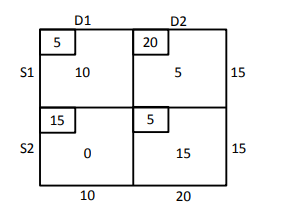
\includegraphics[width=0.75\columnwidth]{chapters/10/7/2/4/figs/fig.png}
 \end{center}
\caption{}
\label{fig:10/7/2/4Fig1}
\end{figure}
\fi

\item Find the position vector of the mid point of the vector joining the points $\vec{P}$(2, 3, 4)
and $\vec{Q}$(4, 1, –2).
\\
\solution
		\begin{enumerate}[label=\thesubsection.\arabic*,ref=\thesubsection.\theenumi]
\item Find the coordinates of the point which divides the join of $(-1,7) $ and $ (4,-3)$ in the ratio 2:3.
	\\
		\solution
	\input{chapters/10/7/2/1/section.tex}
\item Find the coordinates of the point $\vec{R}$ on the line segment joining the points $\vec{P}(-1,3)$ and $\vec{Q}(2,5)$ such that $PR=\frac{3}{5}PQ$.
\item Find the ratio in which the point $\vec{P}\brak{\frac{3}{4},\frac{5}{12}}$ divides the line segment joining the points $\vec{A}\brak{\frac{1}{2},\frac{3}{2}}$ and $ \vec{B}(2,-5)$.
\item Find the coordinates of the point which divides the line segment joining the points $(4,-3)$ and $(8,5)$ in the ratio $3:1$ internally.
\item Find the coordinates of the point $\vec{P}$ on $AD$ such that $AP : PD = 2 : 1$.
\item If the point $\vec{P} (2, 1)$ lies on the line segment joining points $\vec{A} (4, 2)$  and $ \vec{B} (8, 4)$,
then
\begin{enumerate}
	\item $AP =\frac{1}{3}{AB}$ 
\item ${AP}={PE}$
\item ${PB}=\frac{1}{3}{AB}$
\item${AP}=\frac{1}{2}{AB}$
 \end{enumerate}
\item Find the ratio in which the line segment joining the points $(-3,10)$  and  $(6,-8)$  is divided by $ (-1,6)$.
	\\
		\solution
	\input{chapters/10/7/2/4/section.tex}
\item Find the position vector of the mid point of the vector joining the points $\vec{P}$(2, 3, 4)
and $\vec{Q}$(4, 1, –2).
\\
\solution
		\input{chapters/12/10/2/16/section.tex}
\item Let $\vec{A}(4, 2), \vec{B}(6, 5)$  and $ \vec{C}(1, 4)$ be the vertices of $\triangle ABC$.
\begin{enumerate}
\item If $\vec{A}$ and  $\vec{B}$ are $(-2,-2)$ and  $(2,-4)$, respectively, find the coordinates of $\vec{P}$ such that $AP= \frac {3}{7}AB$  and $ \vec{P}$ lies on the line segment $AB$.
	\\
		\solution
	\input{chapters/10/7/2/8/section.tex}
\item Find the coordinates of the points which divide the line segment joining $A(-2,2)$  and  $\vec{B}(2,8)$ into four equal parts.
	\\
		\solution
	\input{chapters/10/7/2/9/section.tex}
\item In what ratio does the point $(-4,6)$ divide the line segment joining the points $\vec{A}(-6,0)$ and $\vec{B}(3,-8)$?
\item Given that $\vec{P}(3,2,-4), \vec{Q}(5,4,-6)$ and $\vec{R}(9,8,-10)$ are collinear. Find the ratio in which $\vec{Q}$ divides $PR$.
\item Points $\vec{A}(-6,10),\vec{B}(-4,6)$  and  $\vec{C}(3,-8)$ are collinear such that $AB=  \frac{2}{9}AC$.
\item The point which divides the line segment joining the points $\vec{P} (7, –6) $  and  $\vec{Q}(3, 4)$ in the 
ratio 1 : 2 internally lies in  which quadrant?
\item Find the coordinates of the points of trisection of the line segment joining $(4,-1)$  and  $(-2,3)$.
	\\
		\solution
	\input{chapters/10/7/2/2/section.tex}
\item Find the coordinates of the points which trisect the line segment joining the points $\vec{P}(4,2,-6)$ and $\vec{Q}(10,-16,6)$.
\item Find the coordinates of the points of trisection (i.e. points dividing to three equal parts) of the line segment joining the points $\vec{A}(2,-2)$ and $\vec{B}(-7,4)$.
\item Point $\vec{P}(5,-3)$ is one of the two points of trisection of line segment joining the points $\vec{A}(7,-2)$ and $\vec{B}(1,-5)$
\item Find the position vector of a point $\vec{R}$ which divides the line joining two points $\vec{P}$
and $\vec{Q}$ whose position vectors are $\hat{i}+2\hat{j}-\hat{k}$ and $-\hat{i}+\hat{j}+\hat{k}$ respectively, in the
ratio 2 : 1
\begin{enumerate}
    \item  internally
    \item  externally
\end{enumerate}
%\solution
%		\input{chapters/12/10/2/15/section.tex}
\item Find the coordinates of the point which divides the line segment joining the points which divides the line segment joining  the points $(-2,3,5)$ and $(1,-4,6)$ in the ratio 
\begin{enumerate}
\item $2:3$ internally,
\item $2:3$ externally
\end{enumerate}
\item Find the coordinates of the point which divides the line segment joining the points $(1,-2,3)$ and $(3,4,-5)$ in the ratio $2:3$
\begin{enumerate}
\item internally, and
\item externally
\end{enumerate}
\item Consider two points $\vec{P}$ and $\vec{Q}$ with position vectors $\overrightarrow{OP} = 3\overrightarrow{a}-2\overrightarrow{b}$ and $\overrightarrow{OQ}=\overrightarrow{a}+\overrightarrow{b}$. Find the position vector of a point $\vec{R}$ which divides the line joining $\vec{P}$ and $\vec{Q}$ in the ratio $2:1$, 
\begin{enumerate}
\item internally, and 
\item externally.
\end{enumerate}
\item The median from $\vec{A}$ meets $BC$ at $\vec{D}$. Find the coordinates of the point $\vec{D}$.
\item Find the coordinates of points $\vec{Q}$ and $\vec{R}$ on medians $BE$ and $CF$ respectively such that $BQ : QE = 2 : 1$  and  $CR : RF = 2 : 1$.
\item What do you observe?
\item If $\vec{A}, \vec{B}$ and $\vec{C}$  are the vertices of $\triangle ABC$, find the coordinates of the centroid of the triangle.
\end{enumerate}
\solution
	\input{chapters/10/7/4/7/section.tex}
\item If $\vec{P}(9a-2,-b)$ divides line segment joining $\vec{A}(3a+1,-3)$ and $\vec{B}(8a,5)$ in the ratio 3:1, find the values of $a$ and $b$.
\item Find the position vector of a point $\vec{R}$ which divides the line joining two points $\vec{P}$ and $\vec{Q}$ whose position vectors are $2\vec{a}+\vec{b}$ and $\vec{a}-3\vec{b}$ externally in the ratio $1:2$.
\item The position vector of the point which divides the join of points 2$\vec{a}$-3$\vec{b}$ $\text{and}$ $\vec{a}+\vec{b}$ in the ratio 3:1 is \rule{1cm}{0.1pt}.
\item If $\vec{a}$ and $\vec{b}$ are the postion vectors of $\vec{A}$ and $\vec{B}$, respectively, find the position vector of a point $\vec{C}$ in $BA$ produced such that $BC=1.5BA$.
\item Find the position vector of a point $\vec{R}$ which divides the line joining two points $\vec{P}$ and $\vec{Q}$ whose position vectors are $(2\vec{a}+\vec{b})$ and $(\vec{a}-3\vec{b})$
externally in the ratio 1 : 2. Also, show that $\vec{P}$ is the mid point of the line segment $RQ$.
\end{enumerate}

\item Let $\vec{A}(4, 2), \vec{B}(6, 5)$  and $ \vec{C}(1, 4)$ be the vertices of $\triangle ABC$.
\begin{enumerate}
\item If $\vec{A}$ and  $\vec{B}$ are $(-2,-2)$ and  $(2,-4)$, respectively, find the coordinates of $\vec{P}$ such that $AP= \frac {3}{7}AB$  and $ \vec{P}$ lies on the line segment $AB$.
	\\
		\solution
	\begin{enumerate}[label=\thesubsection.\arabic*,ref=\thesubsection.\theenumi]
\item Find the coordinates of the point which divides the join of $(-1,7) $ and $ (4,-3)$ in the ratio 2:3.
	\\
		\solution
	\input{chapters/10/7/2/1/section.tex}
\item Find the coordinates of the point $\vec{R}$ on the line segment joining the points $\vec{P}(-1,3)$ and $\vec{Q}(2,5)$ such that $PR=\frac{3}{5}PQ$.
\item Find the ratio in which the point $\vec{P}\brak{\frac{3}{4},\frac{5}{12}}$ divides the line segment joining the points $\vec{A}\brak{\frac{1}{2},\frac{3}{2}}$ and $ \vec{B}(2,-5)$.
\item Find the coordinates of the point which divides the line segment joining the points $(4,-3)$ and $(8,5)$ in the ratio $3:1$ internally.
\item Find the coordinates of the point $\vec{P}$ on $AD$ such that $AP : PD = 2 : 1$.
\item If the point $\vec{P} (2, 1)$ lies on the line segment joining points $\vec{A} (4, 2)$  and $ \vec{B} (8, 4)$,
then
\begin{enumerate}
	\item $AP =\frac{1}{3}{AB}$ 
\item ${AP}={PE}$
\item ${PB}=\frac{1}{3}{AB}$
\item${AP}=\frac{1}{2}{AB}$
 \end{enumerate}
\item Find the ratio in which the line segment joining the points $(-3,10)$  and  $(6,-8)$  is divided by $ (-1,6)$.
	\\
		\solution
	\input{chapters/10/7/2/4/section.tex}
\item Find the position vector of the mid point of the vector joining the points $\vec{P}$(2, 3, 4)
and $\vec{Q}$(4, 1, –2).
\\
\solution
		\input{chapters/12/10/2/16/section.tex}
\item Let $\vec{A}(4, 2), \vec{B}(6, 5)$  and $ \vec{C}(1, 4)$ be the vertices of $\triangle ABC$.
\begin{enumerate}
\item If $\vec{A}$ and  $\vec{B}$ are $(-2,-2)$ and  $(2,-4)$, respectively, find the coordinates of $\vec{P}$ such that $AP= \frac {3}{7}AB$  and $ \vec{P}$ lies on the line segment $AB$.
	\\
		\solution
	\input{chapters/10/7/2/8/section.tex}
\item Find the coordinates of the points which divide the line segment joining $A(-2,2)$  and  $\vec{B}(2,8)$ into four equal parts.
	\\
		\solution
	\input{chapters/10/7/2/9/section.tex}
\item In what ratio does the point $(-4,6)$ divide the line segment joining the points $\vec{A}(-6,0)$ and $\vec{B}(3,-8)$?
\item Given that $\vec{P}(3,2,-4), \vec{Q}(5,4,-6)$ and $\vec{R}(9,8,-10)$ are collinear. Find the ratio in which $\vec{Q}$ divides $PR$.
\item Points $\vec{A}(-6,10),\vec{B}(-4,6)$  and  $\vec{C}(3,-8)$ are collinear such that $AB=  \frac{2}{9}AC$.
\item The point which divides the line segment joining the points $\vec{P} (7, –6) $  and  $\vec{Q}(3, 4)$ in the 
ratio 1 : 2 internally lies in  which quadrant?
\item Find the coordinates of the points of trisection of the line segment joining $(4,-1)$  and  $(-2,3)$.
	\\
		\solution
	\input{chapters/10/7/2/2/section.tex}
\item Find the coordinates of the points which trisect the line segment joining the points $\vec{P}(4,2,-6)$ and $\vec{Q}(10,-16,6)$.
\item Find the coordinates of the points of trisection (i.e. points dividing to three equal parts) of the line segment joining the points $\vec{A}(2,-2)$ and $\vec{B}(-7,4)$.
\item Point $\vec{P}(5,-3)$ is one of the two points of trisection of line segment joining the points $\vec{A}(7,-2)$ and $\vec{B}(1,-5)$
\item Find the position vector of a point $\vec{R}$ which divides the line joining two points $\vec{P}$
and $\vec{Q}$ whose position vectors are $\hat{i}+2\hat{j}-\hat{k}$ and $-\hat{i}+\hat{j}+\hat{k}$ respectively, in the
ratio 2 : 1
\begin{enumerate}
    \item  internally
    \item  externally
\end{enumerate}
%\solution
%		\input{chapters/12/10/2/15/section.tex}
\item Find the coordinates of the point which divides the line segment joining the points which divides the line segment joining  the points $(-2,3,5)$ and $(1,-4,6)$ in the ratio 
\begin{enumerate}
\item $2:3$ internally,
\item $2:3$ externally
\end{enumerate}
\item Find the coordinates of the point which divides the line segment joining the points $(1,-2,3)$ and $(3,4,-5)$ in the ratio $2:3$
\begin{enumerate}
\item internally, and
\item externally
\end{enumerate}
\item Consider two points $\vec{P}$ and $\vec{Q}$ with position vectors $\overrightarrow{OP} = 3\overrightarrow{a}-2\overrightarrow{b}$ and $\overrightarrow{OQ}=\overrightarrow{a}+\overrightarrow{b}$. Find the position vector of a point $\vec{R}$ which divides the line joining $\vec{P}$ and $\vec{Q}$ in the ratio $2:1$, 
\begin{enumerate}
\item internally, and 
\item externally.
\end{enumerate}
\item The median from $\vec{A}$ meets $BC$ at $\vec{D}$. Find the coordinates of the point $\vec{D}$.
\item Find the coordinates of points $\vec{Q}$ and $\vec{R}$ on medians $BE$ and $CF$ respectively such that $BQ : QE = 2 : 1$  and  $CR : RF = 2 : 1$.
\item What do you observe?
\item If $\vec{A}, \vec{B}$ and $\vec{C}$  are the vertices of $\triangle ABC$, find the coordinates of the centroid of the triangle.
\end{enumerate}
\solution
	\input{chapters/10/7/4/7/section.tex}
\item If $\vec{P}(9a-2,-b)$ divides line segment joining $\vec{A}(3a+1,-3)$ and $\vec{B}(8a,5)$ in the ratio 3:1, find the values of $a$ and $b$.
\item Find the position vector of a point $\vec{R}$ which divides the line joining two points $\vec{P}$ and $\vec{Q}$ whose position vectors are $2\vec{a}+\vec{b}$ and $\vec{a}-3\vec{b}$ externally in the ratio $1:2$.
\item The position vector of the point which divides the join of points 2$\vec{a}$-3$\vec{b}$ $\text{and}$ $\vec{a}+\vec{b}$ in the ratio 3:1 is \rule{1cm}{0.1pt}.
\item If $\vec{a}$ and $\vec{b}$ are the postion vectors of $\vec{A}$ and $\vec{B}$, respectively, find the position vector of a point $\vec{C}$ in $BA$ produced such that $BC=1.5BA$.
\item Find the position vector of a point $\vec{R}$ which divides the line joining two points $\vec{P}$ and $\vec{Q}$ whose position vectors are $(2\vec{a}+\vec{b})$ and $(\vec{a}-3\vec{b})$
externally in the ratio 1 : 2. Also, show that $\vec{P}$ is the mid point of the line segment $RQ$.
\end{enumerate}

\item Find the coordinates of the points which divide the line segment joining $A(-2,2)$  and  $\vec{B}(2,8)$ into four equal parts.
	\\
		\solution
	\begin{enumerate}[label=\thesubsection.\arabic*,ref=\thesubsection.\theenumi]
\item Find the coordinates of the point which divides the join of $(-1,7) $ and $ (4,-3)$ in the ratio 2:3.
	\\
		\solution
	\input{chapters/10/7/2/1/section.tex}
\item Find the coordinates of the point $\vec{R}$ on the line segment joining the points $\vec{P}(-1,3)$ and $\vec{Q}(2,5)$ such that $PR=\frac{3}{5}PQ$.
\item Find the ratio in which the point $\vec{P}\brak{\frac{3}{4},\frac{5}{12}}$ divides the line segment joining the points $\vec{A}\brak{\frac{1}{2},\frac{3}{2}}$ and $ \vec{B}(2,-5)$.
\item Find the coordinates of the point which divides the line segment joining the points $(4,-3)$ and $(8,5)$ in the ratio $3:1$ internally.
\item Find the coordinates of the point $\vec{P}$ on $AD$ such that $AP : PD = 2 : 1$.
\item If the point $\vec{P} (2, 1)$ lies on the line segment joining points $\vec{A} (4, 2)$  and $ \vec{B} (8, 4)$,
then
\begin{enumerate}
	\item $AP =\frac{1}{3}{AB}$ 
\item ${AP}={PE}$
\item ${PB}=\frac{1}{3}{AB}$
\item${AP}=\frac{1}{2}{AB}$
 \end{enumerate}
\item Find the ratio in which the line segment joining the points $(-3,10)$  and  $(6,-8)$  is divided by $ (-1,6)$.
	\\
		\solution
	\input{chapters/10/7/2/4/section.tex}
\item Find the position vector of the mid point of the vector joining the points $\vec{P}$(2, 3, 4)
and $\vec{Q}$(4, 1, –2).
\\
\solution
		\input{chapters/12/10/2/16/section.tex}
\item Let $\vec{A}(4, 2), \vec{B}(6, 5)$  and $ \vec{C}(1, 4)$ be the vertices of $\triangle ABC$.
\begin{enumerate}
\item If $\vec{A}$ and  $\vec{B}$ are $(-2,-2)$ and  $(2,-4)$, respectively, find the coordinates of $\vec{P}$ such that $AP= \frac {3}{7}AB$  and $ \vec{P}$ lies on the line segment $AB$.
	\\
		\solution
	\input{chapters/10/7/2/8/section.tex}
\item Find the coordinates of the points which divide the line segment joining $A(-2,2)$  and  $\vec{B}(2,8)$ into four equal parts.
	\\
		\solution
	\input{chapters/10/7/2/9/section.tex}
\item In what ratio does the point $(-4,6)$ divide the line segment joining the points $\vec{A}(-6,0)$ and $\vec{B}(3,-8)$?
\item Given that $\vec{P}(3,2,-4), \vec{Q}(5,4,-6)$ and $\vec{R}(9,8,-10)$ are collinear. Find the ratio in which $\vec{Q}$ divides $PR$.
\item Points $\vec{A}(-6,10),\vec{B}(-4,6)$  and  $\vec{C}(3,-8)$ are collinear such that $AB=  \frac{2}{9}AC$.
\item The point which divides the line segment joining the points $\vec{P} (7, –6) $  and  $\vec{Q}(3, 4)$ in the 
ratio 1 : 2 internally lies in  which quadrant?
\item Find the coordinates of the points of trisection of the line segment joining $(4,-1)$  and  $(-2,3)$.
	\\
		\solution
	\input{chapters/10/7/2/2/section.tex}
\item Find the coordinates of the points which trisect the line segment joining the points $\vec{P}(4,2,-6)$ and $\vec{Q}(10,-16,6)$.
\item Find the coordinates of the points of trisection (i.e. points dividing to three equal parts) of the line segment joining the points $\vec{A}(2,-2)$ and $\vec{B}(-7,4)$.
\item Point $\vec{P}(5,-3)$ is one of the two points of trisection of line segment joining the points $\vec{A}(7,-2)$ and $\vec{B}(1,-5)$
\item Find the position vector of a point $\vec{R}$ which divides the line joining two points $\vec{P}$
and $\vec{Q}$ whose position vectors are $\hat{i}+2\hat{j}-\hat{k}$ and $-\hat{i}+\hat{j}+\hat{k}$ respectively, in the
ratio 2 : 1
\begin{enumerate}
    \item  internally
    \item  externally
\end{enumerate}
%\solution
%		\input{chapters/12/10/2/15/section.tex}
\item Find the coordinates of the point which divides the line segment joining the points which divides the line segment joining  the points $(-2,3,5)$ and $(1,-4,6)$ in the ratio 
\begin{enumerate}
\item $2:3$ internally,
\item $2:3$ externally
\end{enumerate}
\item Find the coordinates of the point which divides the line segment joining the points $(1,-2,3)$ and $(3,4,-5)$ in the ratio $2:3$
\begin{enumerate}
\item internally, and
\item externally
\end{enumerate}
\item Consider two points $\vec{P}$ and $\vec{Q}$ with position vectors $\overrightarrow{OP} = 3\overrightarrow{a}-2\overrightarrow{b}$ and $\overrightarrow{OQ}=\overrightarrow{a}+\overrightarrow{b}$. Find the position vector of a point $\vec{R}$ which divides the line joining $\vec{P}$ and $\vec{Q}$ in the ratio $2:1$, 
\begin{enumerate}
\item internally, and 
\item externally.
\end{enumerate}
\item The median from $\vec{A}$ meets $BC$ at $\vec{D}$. Find the coordinates of the point $\vec{D}$.
\item Find the coordinates of points $\vec{Q}$ and $\vec{R}$ on medians $BE$ and $CF$ respectively such that $BQ : QE = 2 : 1$  and  $CR : RF = 2 : 1$.
\item What do you observe?
\item If $\vec{A}, \vec{B}$ and $\vec{C}$  are the vertices of $\triangle ABC$, find the coordinates of the centroid of the triangle.
\end{enumerate}
\solution
	\input{chapters/10/7/4/7/section.tex}
\item If $\vec{P}(9a-2,-b)$ divides line segment joining $\vec{A}(3a+1,-3)$ and $\vec{B}(8a,5)$ in the ratio 3:1, find the values of $a$ and $b$.
\item Find the position vector of a point $\vec{R}$ which divides the line joining two points $\vec{P}$ and $\vec{Q}$ whose position vectors are $2\vec{a}+\vec{b}$ and $\vec{a}-3\vec{b}$ externally in the ratio $1:2$.
\item The position vector of the point which divides the join of points 2$\vec{a}$-3$\vec{b}$ $\text{and}$ $\vec{a}+\vec{b}$ in the ratio 3:1 is \rule{1cm}{0.1pt}.
\item If $\vec{a}$ and $\vec{b}$ are the postion vectors of $\vec{A}$ and $\vec{B}$, respectively, find the position vector of a point $\vec{C}$ in $BA$ produced such that $BC=1.5BA$.
\item Find the position vector of a point $\vec{R}$ which divides the line joining two points $\vec{P}$ and $\vec{Q}$ whose position vectors are $(2\vec{a}+\vec{b})$ and $(\vec{a}-3\vec{b})$
externally in the ratio 1 : 2. Also, show that $\vec{P}$ is the mid point of the line segment $RQ$.
\end{enumerate}

\item In what ratio does the point $(-4,6)$ divide the line segment joining the points $\vec{A}(-6,0)$ and $\vec{B}(3,-8)$?
\item Given that $\vec{P}(3,2,-4), \vec{Q}(5,4,-6)$ and $\vec{R}(9,8,-10)$ are collinear. Find the ratio in which $\vec{Q}$ divides $PR$.
\item Points $\vec{A}(-6,10),\vec{B}(-4,6)$  and  $\vec{C}(3,-8)$ are collinear such that $AB=  \frac{2}{9}AC$.
\item The point which divides the line segment joining the points $\vec{P} (7, –6) $  and  $\vec{Q}(3, 4)$ in the 
ratio 1 : 2 internally lies in  which quadrant?
\item Find the coordinates of the points of trisection of the line segment joining $(4,-1)$  and  $(-2,3)$.
	\\
		\solution
	Using section formula,
\begin{align}
\vec{R}=\frac{1}{1+\frac{1}{2}}\brak{\myvec{4\\-1}+\frac{1}{2}\myvec{-2\\3}}
=\myvec{2\\ \frac{1}{3}}\\
\vec{S}=\frac{1}{1+\frac{2}{1}}\brak{\myvec{4\\-1}+\frac{2}{1}\myvec{-2\\3}}
=\myvec{0\\ \frac{5}{3}}
\end{align}
which are the desired points of trisection.
\iffalse
See
		\figref{fig:chapters/10/7/2/2/Figure}
\begin{figure}[H]
\centering
\includegraphics[width=0.75\columnwidth]{chapters/10/7/2/2/figs/dj.pdf}
\caption{}
		\label{fig:chapters/10/7/2/2/Figure}
\end{figure}
\fi

\item Find the coordinates of the points which trisect the line segment joining the points $\vec{P}(4,2,-6)$ and $\vec{Q}(10,-16,6)$.
\item Find the coordinates of the points of trisection (i.e. points dividing to three equal parts) of the line segment joining the points $\vec{A}(2,-2)$ and $\vec{B}(-7,4)$.
\item Point $\vec{P}(5,-3)$ is one of the two points of trisection of line segment joining the points $\vec{A}(7,-2)$ and $\vec{B}(1,-5)$
\item Find the position vector of a point $\vec{R}$ which divides the line joining two points $\vec{P}$
and $\vec{Q}$ whose position vectors are $\hat{i}+2\hat{j}-\hat{k}$ and $-\hat{i}+\hat{j}+\hat{k}$ respectively, in the
ratio 2 : 1
\begin{enumerate}
    \item  internally
    \item  externally
\end{enumerate}
%\solution
%		\begin{enumerate}[label=\thesubsection.\arabic*,ref=\thesubsection.\theenumi]
\item Find the coordinates of the point which divides the join of $(-1,7) $ and $ (4,-3)$ in the ratio 2:3.
	\\
		\solution
	\input{chapters/10/7/2/1/section.tex}
\item Find the coordinates of the point $\vec{R}$ on the line segment joining the points $\vec{P}(-1,3)$ and $\vec{Q}(2,5)$ such that $PR=\frac{3}{5}PQ$.
\item Find the ratio in which the point $\vec{P}\brak{\frac{3}{4},\frac{5}{12}}$ divides the line segment joining the points $\vec{A}\brak{\frac{1}{2},\frac{3}{2}}$ and $ \vec{B}(2,-5)$.
\item Find the coordinates of the point which divides the line segment joining the points $(4,-3)$ and $(8,5)$ in the ratio $3:1$ internally.
\item Find the coordinates of the point $\vec{P}$ on $AD$ such that $AP : PD = 2 : 1$.
\item If the point $\vec{P} (2, 1)$ lies on the line segment joining points $\vec{A} (4, 2)$  and $ \vec{B} (8, 4)$,
then
\begin{enumerate}
	\item $AP =\frac{1}{3}{AB}$ 
\item ${AP}={PE}$
\item ${PB}=\frac{1}{3}{AB}$
\item${AP}=\frac{1}{2}{AB}$
 \end{enumerate}
\item Find the ratio in which the line segment joining the points $(-3,10)$  and  $(6,-8)$  is divided by $ (-1,6)$.
	\\
		\solution
	\input{chapters/10/7/2/4/section.tex}
\item Find the position vector of the mid point of the vector joining the points $\vec{P}$(2, 3, 4)
and $\vec{Q}$(4, 1, –2).
\\
\solution
		\input{chapters/12/10/2/16/section.tex}
\item Let $\vec{A}(4, 2), \vec{B}(6, 5)$  and $ \vec{C}(1, 4)$ be the vertices of $\triangle ABC$.
\begin{enumerate}
\item If $\vec{A}$ and  $\vec{B}$ are $(-2,-2)$ and  $(2,-4)$, respectively, find the coordinates of $\vec{P}$ such that $AP= \frac {3}{7}AB$  and $ \vec{P}$ lies on the line segment $AB$.
	\\
		\solution
	\input{chapters/10/7/2/8/section.tex}
\item Find the coordinates of the points which divide the line segment joining $A(-2,2)$  and  $\vec{B}(2,8)$ into four equal parts.
	\\
		\solution
	\input{chapters/10/7/2/9/section.tex}
\item In what ratio does the point $(-4,6)$ divide the line segment joining the points $\vec{A}(-6,0)$ and $\vec{B}(3,-8)$?
\item Given that $\vec{P}(3,2,-4), \vec{Q}(5,4,-6)$ and $\vec{R}(9,8,-10)$ are collinear. Find the ratio in which $\vec{Q}$ divides $PR$.
\item Points $\vec{A}(-6,10),\vec{B}(-4,6)$  and  $\vec{C}(3,-8)$ are collinear such that $AB=  \frac{2}{9}AC$.
\item The point which divides the line segment joining the points $\vec{P} (7, –6) $  and  $\vec{Q}(3, 4)$ in the 
ratio 1 : 2 internally lies in  which quadrant?
\item Find the coordinates of the points of trisection of the line segment joining $(4,-1)$  and  $(-2,3)$.
	\\
		\solution
	\input{chapters/10/7/2/2/section.tex}
\item Find the coordinates of the points which trisect the line segment joining the points $\vec{P}(4,2,-6)$ and $\vec{Q}(10,-16,6)$.
\item Find the coordinates of the points of trisection (i.e. points dividing to three equal parts) of the line segment joining the points $\vec{A}(2,-2)$ and $\vec{B}(-7,4)$.
\item Point $\vec{P}(5,-3)$ is one of the two points of trisection of line segment joining the points $\vec{A}(7,-2)$ and $\vec{B}(1,-5)$
\item Find the position vector of a point $\vec{R}$ which divides the line joining two points $\vec{P}$
and $\vec{Q}$ whose position vectors are $\hat{i}+2\hat{j}-\hat{k}$ and $-\hat{i}+\hat{j}+\hat{k}$ respectively, in the
ratio 2 : 1
\begin{enumerate}
    \item  internally
    \item  externally
\end{enumerate}
%\solution
%		\input{chapters/12/10/2/15/section.tex}
\item Find the coordinates of the point which divides the line segment joining the points which divides the line segment joining  the points $(-2,3,5)$ and $(1,-4,6)$ in the ratio 
\begin{enumerate}
\item $2:3$ internally,
\item $2:3$ externally
\end{enumerate}
\item Find the coordinates of the point which divides the line segment joining the points $(1,-2,3)$ and $(3,4,-5)$ in the ratio $2:3$
\begin{enumerate}
\item internally, and
\item externally
\end{enumerate}
\item Consider two points $\vec{P}$ and $\vec{Q}$ with position vectors $\overrightarrow{OP} = 3\overrightarrow{a}-2\overrightarrow{b}$ and $\overrightarrow{OQ}=\overrightarrow{a}+\overrightarrow{b}$. Find the position vector of a point $\vec{R}$ which divides the line joining $\vec{P}$ and $\vec{Q}$ in the ratio $2:1$, 
\begin{enumerate}
\item internally, and 
\item externally.
\end{enumerate}
\item The median from $\vec{A}$ meets $BC$ at $\vec{D}$. Find the coordinates of the point $\vec{D}$.
\item Find the coordinates of points $\vec{Q}$ and $\vec{R}$ on medians $BE$ and $CF$ respectively such that $BQ : QE = 2 : 1$  and  $CR : RF = 2 : 1$.
\item What do you observe?
\item If $\vec{A}, \vec{B}$ and $\vec{C}$  are the vertices of $\triangle ABC$, find the coordinates of the centroid of the triangle.
\end{enumerate}
\solution
	\input{chapters/10/7/4/7/section.tex}
\item If $\vec{P}(9a-2,-b)$ divides line segment joining $\vec{A}(3a+1,-3)$ and $\vec{B}(8a,5)$ in the ratio 3:1, find the values of $a$ and $b$.
\item Find the position vector of a point $\vec{R}$ which divides the line joining two points $\vec{P}$ and $\vec{Q}$ whose position vectors are $2\vec{a}+\vec{b}$ and $\vec{a}-3\vec{b}$ externally in the ratio $1:2$.
\item The position vector of the point which divides the join of points 2$\vec{a}$-3$\vec{b}$ $\text{and}$ $\vec{a}+\vec{b}$ in the ratio 3:1 is \rule{1cm}{0.1pt}.
\item If $\vec{a}$ and $\vec{b}$ are the postion vectors of $\vec{A}$ and $\vec{B}$, respectively, find the position vector of a point $\vec{C}$ in $BA$ produced such that $BC=1.5BA$.
\item Find the position vector of a point $\vec{R}$ which divides the line joining two points $\vec{P}$ and $\vec{Q}$ whose position vectors are $(2\vec{a}+\vec{b})$ and $(\vec{a}-3\vec{b})$
externally in the ratio 1 : 2. Also, show that $\vec{P}$ is the mid point of the line segment $RQ$.
\end{enumerate}

\item Find the coordinates of the point which divides the line segment joining the points which divides the line segment joining  the points $(-2,3,5)$ and $(1,-4,6)$ in the ratio 
\begin{enumerate}
\item $2:3$ internally,
\item $2:3$ externally
\end{enumerate}
\item Find the coordinates of the point which divides the line segment joining the points $(1,-2,3)$ and $(3,4,-5)$ in the ratio $2:3$
\begin{enumerate}
\item internally, and
\item externally
\end{enumerate}
\item Consider two points $\vec{P}$ and $\vec{Q}$ with position vectors $\overrightarrow{OP} = 3\overrightarrow{a}-2\overrightarrow{b}$ and $\overrightarrow{OQ}=\overrightarrow{a}+\overrightarrow{b}$. Find the position vector of a point $\vec{R}$ which divides the line joining $\vec{P}$ and $\vec{Q}$ in the ratio $2:1$, 
\begin{enumerate}
\item internally, and 
\item externally.
\end{enumerate}
\item The median from $\vec{A}$ meets $BC$ at $\vec{D}$. Find the coordinates of the point $\vec{D}$.
\item Find the coordinates of points $\vec{Q}$ and $\vec{R}$ on medians $BE$ and $CF$ respectively such that $BQ : QE = 2 : 1$  and  $CR : RF = 2 : 1$.
\item What do you observe?
\item If $\vec{A}, \vec{B}$ and $\vec{C}$  are the vertices of $\triangle ABC$, find the coordinates of the centroid of the triangle.
\end{enumerate}
\solution
	\begin{enumerate}[label=\thesubsection.\arabic*,ref=\thesubsection.\theenumi]
\item Find the coordinates of the point which divides the join of $(-1,7) $ and $ (4,-3)$ in the ratio 2:3.
	\\
		\solution
	\input{chapters/10/7/2/1/section.tex}
\item Find the coordinates of the point $\vec{R}$ on the line segment joining the points $\vec{P}(-1,3)$ and $\vec{Q}(2,5)$ such that $PR=\frac{3}{5}PQ$.
\item Find the ratio in which the point $\vec{P}\brak{\frac{3}{4},\frac{5}{12}}$ divides the line segment joining the points $\vec{A}\brak{\frac{1}{2},\frac{3}{2}}$ and $ \vec{B}(2,-5)$.
\item Find the coordinates of the point which divides the line segment joining the points $(4,-3)$ and $(8,5)$ in the ratio $3:1$ internally.
\item Find the coordinates of the point $\vec{P}$ on $AD$ such that $AP : PD = 2 : 1$.
\item If the point $\vec{P} (2, 1)$ lies on the line segment joining points $\vec{A} (4, 2)$  and $ \vec{B} (8, 4)$,
then
\begin{enumerate}
	\item $AP =\frac{1}{3}{AB}$ 
\item ${AP}={PE}$
\item ${PB}=\frac{1}{3}{AB}$
\item${AP}=\frac{1}{2}{AB}$
 \end{enumerate}
\item Find the ratio in which the line segment joining the points $(-3,10)$  and  $(6,-8)$  is divided by $ (-1,6)$.
	\\
		\solution
	\input{chapters/10/7/2/4/section.tex}
\item Find the position vector of the mid point of the vector joining the points $\vec{P}$(2, 3, 4)
and $\vec{Q}$(4, 1, –2).
\\
\solution
		\input{chapters/12/10/2/16/section.tex}
\item Let $\vec{A}(4, 2), \vec{B}(6, 5)$  and $ \vec{C}(1, 4)$ be the vertices of $\triangle ABC$.
\begin{enumerate}
\item If $\vec{A}$ and  $\vec{B}$ are $(-2,-2)$ and  $(2,-4)$, respectively, find the coordinates of $\vec{P}$ such that $AP= \frac {3}{7}AB$  and $ \vec{P}$ lies on the line segment $AB$.
	\\
		\solution
	\input{chapters/10/7/2/8/section.tex}
\item Find the coordinates of the points which divide the line segment joining $A(-2,2)$  and  $\vec{B}(2,8)$ into four equal parts.
	\\
		\solution
	\input{chapters/10/7/2/9/section.tex}
\item In what ratio does the point $(-4,6)$ divide the line segment joining the points $\vec{A}(-6,0)$ and $\vec{B}(3,-8)$?
\item Given that $\vec{P}(3,2,-4), \vec{Q}(5,4,-6)$ and $\vec{R}(9,8,-10)$ are collinear. Find the ratio in which $\vec{Q}$ divides $PR$.
\item Points $\vec{A}(-6,10),\vec{B}(-4,6)$  and  $\vec{C}(3,-8)$ are collinear such that $AB=  \frac{2}{9}AC$.
\item The point which divides the line segment joining the points $\vec{P} (7, –6) $  and  $\vec{Q}(3, 4)$ in the 
ratio 1 : 2 internally lies in  which quadrant?
\item Find the coordinates of the points of trisection of the line segment joining $(4,-1)$  and  $(-2,3)$.
	\\
		\solution
	\input{chapters/10/7/2/2/section.tex}
\item Find the coordinates of the points which trisect the line segment joining the points $\vec{P}(4,2,-6)$ and $\vec{Q}(10,-16,6)$.
\item Find the coordinates of the points of trisection (i.e. points dividing to three equal parts) of the line segment joining the points $\vec{A}(2,-2)$ and $\vec{B}(-7,4)$.
\item Point $\vec{P}(5,-3)$ is one of the two points of trisection of line segment joining the points $\vec{A}(7,-2)$ and $\vec{B}(1,-5)$
\item Find the position vector of a point $\vec{R}$ which divides the line joining two points $\vec{P}$
and $\vec{Q}$ whose position vectors are $\hat{i}+2\hat{j}-\hat{k}$ and $-\hat{i}+\hat{j}+\hat{k}$ respectively, in the
ratio 2 : 1
\begin{enumerate}
    \item  internally
    \item  externally
\end{enumerate}
%\solution
%		\input{chapters/12/10/2/15/section.tex}
\item Find the coordinates of the point which divides the line segment joining the points which divides the line segment joining  the points $(-2,3,5)$ and $(1,-4,6)$ in the ratio 
\begin{enumerate}
\item $2:3$ internally,
\item $2:3$ externally
\end{enumerate}
\item Find the coordinates of the point which divides the line segment joining the points $(1,-2,3)$ and $(3,4,-5)$ in the ratio $2:3$
\begin{enumerate}
\item internally, and
\item externally
\end{enumerate}
\item Consider two points $\vec{P}$ and $\vec{Q}$ with position vectors $\overrightarrow{OP} = 3\overrightarrow{a}-2\overrightarrow{b}$ and $\overrightarrow{OQ}=\overrightarrow{a}+\overrightarrow{b}$. Find the position vector of a point $\vec{R}$ which divides the line joining $\vec{P}$ and $\vec{Q}$ in the ratio $2:1$, 
\begin{enumerate}
\item internally, and 
\item externally.
\end{enumerate}
\item The median from $\vec{A}$ meets $BC$ at $\vec{D}$. Find the coordinates of the point $\vec{D}$.
\item Find the coordinates of points $\vec{Q}$ and $\vec{R}$ on medians $BE$ and $CF$ respectively such that $BQ : QE = 2 : 1$  and  $CR : RF = 2 : 1$.
\item What do you observe?
\item If $\vec{A}, \vec{B}$ and $\vec{C}$  are the vertices of $\triangle ABC$, find the coordinates of the centroid of the triangle.
\end{enumerate}
\solution
	\input{chapters/10/7/4/7/section.tex}
\item If $\vec{P}(9a-2,-b)$ divides line segment joining $\vec{A}(3a+1,-3)$ and $\vec{B}(8a,5)$ in the ratio 3:1, find the values of $a$ and $b$.
\item Find the position vector of a point $\vec{R}$ which divides the line joining two points $\vec{P}$ and $\vec{Q}$ whose position vectors are $2\vec{a}+\vec{b}$ and $\vec{a}-3\vec{b}$ externally in the ratio $1:2$.
\item The position vector of the point which divides the join of points 2$\vec{a}$-3$\vec{b}$ $\text{and}$ $\vec{a}+\vec{b}$ in the ratio 3:1 is \rule{1cm}{0.1pt}.
\item If $\vec{a}$ and $\vec{b}$ are the postion vectors of $\vec{A}$ and $\vec{B}$, respectively, find the position vector of a point $\vec{C}$ in $BA$ produced such that $BC=1.5BA$.
\item Find the position vector of a point $\vec{R}$ which divides the line joining two points $\vec{P}$ and $\vec{Q}$ whose position vectors are $(2\vec{a}+\vec{b})$ and $(\vec{a}-3\vec{b})$
externally in the ratio 1 : 2. Also, show that $\vec{P}$ is the mid point of the line segment $RQ$.
\end{enumerate}

\item If $\vec{P}(9a-2,-b)$ divides line segment joining $\vec{A}(3a+1,-3)$ and $\vec{B}(8a,5)$ in the ratio 3:1, find the values of $a$ and $b$.
\item Find the position vector of a point $\vec{R}$ which divides the line joining two points $\vec{P}$ and $\vec{Q}$ whose position vectors are $2\vec{a}+\vec{b}$ and $\vec{a}-3\vec{b}$ externally in the ratio $1:2$.
\item The position vector of the point which divides the join of points 2$\vec{a}$-3$\vec{b}$ $\text{and}$ $\vec{a}+\vec{b}$ in the ratio 3:1 is \rule{1cm}{0.1pt}.
\item If $\vec{a}$ and $\vec{b}$ are the postion vectors of $\vec{A}$ and $\vec{B}$, respectively, find the position vector of a point $\vec{C}$ in $BA$ produced such that $BC=1.5BA$.
\item Find the position vector of a point $\vec{R}$ which divides the line joining two points $\vec{P}$ and $\vec{Q}$ whose position vectors are $(2\vec{a}+\vec{b})$ and $(\vec{a}-3\vec{b})$
externally in the ratio 1 : 2. Also, show that $\vec{P}$ is the mid point of the line segment $RQ$.
\end{enumerate}

\item Find the coordinates of the points which divide the line segment joining $A(-2,2)$  and  $\vec{B}(2,8)$ into four equal parts.
	\\
		\solution
	\begin{enumerate}[label=\thesubsection.\arabic*,ref=\thesubsection.\theenumi]
\item Find the coordinates of the point which divides the join of $(-1,7) $ and $ (4,-3)$ in the ratio 2:3.
	\\
		\solution
	\begin{enumerate}[label=\thesubsection.\arabic*,ref=\thesubsection.\theenumi]
\item Find the coordinates of the point which divides the join of $(-1,7) $ and $ (4,-3)$ in the ratio 2:3.
	\\
		\solution
	\input{chapters/10/7/2/1/section.tex}
\item Find the coordinates of the point $\vec{R}$ on the line segment joining the points $\vec{P}(-1,3)$ and $\vec{Q}(2,5)$ such that $PR=\frac{3}{5}PQ$.
\item Find the ratio in which the point $\vec{P}\brak{\frac{3}{4},\frac{5}{12}}$ divides the line segment joining the points $\vec{A}\brak{\frac{1}{2},\frac{3}{2}}$ and $ \vec{B}(2,-5)$.
\item Find the coordinates of the point which divides the line segment joining the points $(4,-3)$ and $(8,5)$ in the ratio $3:1$ internally.
\item Find the coordinates of the point $\vec{P}$ on $AD$ such that $AP : PD = 2 : 1$.
\item If the point $\vec{P} (2, 1)$ lies on the line segment joining points $\vec{A} (4, 2)$  and $ \vec{B} (8, 4)$,
then
\begin{enumerate}
	\item $AP =\frac{1}{3}{AB}$ 
\item ${AP}={PE}$
\item ${PB}=\frac{1}{3}{AB}$
\item${AP}=\frac{1}{2}{AB}$
 \end{enumerate}
\item Find the ratio in which the line segment joining the points $(-3,10)$  and  $(6,-8)$  is divided by $ (-1,6)$.
	\\
		\solution
	\input{chapters/10/7/2/4/section.tex}
\item Find the position vector of the mid point of the vector joining the points $\vec{P}$(2, 3, 4)
and $\vec{Q}$(4, 1, –2).
\\
\solution
		\input{chapters/12/10/2/16/section.tex}
\item Let $\vec{A}(4, 2), \vec{B}(6, 5)$  and $ \vec{C}(1, 4)$ be the vertices of $\triangle ABC$.
\begin{enumerate}
\item If $\vec{A}$ and  $\vec{B}$ are $(-2,-2)$ and  $(2,-4)$, respectively, find the coordinates of $\vec{P}$ such that $AP= \frac {3}{7}AB$  and $ \vec{P}$ lies on the line segment $AB$.
	\\
		\solution
	\input{chapters/10/7/2/8/section.tex}
\item Find the coordinates of the points which divide the line segment joining $A(-2,2)$  and  $\vec{B}(2,8)$ into four equal parts.
	\\
		\solution
	\input{chapters/10/7/2/9/section.tex}
\item In what ratio does the point $(-4,6)$ divide the line segment joining the points $\vec{A}(-6,0)$ and $\vec{B}(3,-8)$?
\item Given that $\vec{P}(3,2,-4), \vec{Q}(5,4,-6)$ and $\vec{R}(9,8,-10)$ are collinear. Find the ratio in which $\vec{Q}$ divides $PR$.
\item Points $\vec{A}(-6,10),\vec{B}(-4,6)$  and  $\vec{C}(3,-8)$ are collinear such that $AB=  \frac{2}{9}AC$.
\item The point which divides the line segment joining the points $\vec{P} (7, –6) $  and  $\vec{Q}(3, 4)$ in the 
ratio 1 : 2 internally lies in  which quadrant?
\item Find the coordinates of the points of trisection of the line segment joining $(4,-1)$  and  $(-2,3)$.
	\\
		\solution
	\input{chapters/10/7/2/2/section.tex}
\item Find the coordinates of the points which trisect the line segment joining the points $\vec{P}(4,2,-6)$ and $\vec{Q}(10,-16,6)$.
\item Find the coordinates of the points of trisection (i.e. points dividing to three equal parts) of the line segment joining the points $\vec{A}(2,-2)$ and $\vec{B}(-7,4)$.
\item Point $\vec{P}(5,-3)$ is one of the two points of trisection of line segment joining the points $\vec{A}(7,-2)$ and $\vec{B}(1,-5)$
\item Find the position vector of a point $\vec{R}$ which divides the line joining two points $\vec{P}$
and $\vec{Q}$ whose position vectors are $\hat{i}+2\hat{j}-\hat{k}$ and $-\hat{i}+\hat{j}+\hat{k}$ respectively, in the
ratio 2 : 1
\begin{enumerate}
    \item  internally
    \item  externally
\end{enumerate}
%\solution
%		\input{chapters/12/10/2/15/section.tex}
\item Find the coordinates of the point which divides the line segment joining the points which divides the line segment joining  the points $(-2,3,5)$ and $(1,-4,6)$ in the ratio 
\begin{enumerate}
\item $2:3$ internally,
\item $2:3$ externally
\end{enumerate}
\item Find the coordinates of the point which divides the line segment joining the points $(1,-2,3)$ and $(3,4,-5)$ in the ratio $2:3$
\begin{enumerate}
\item internally, and
\item externally
\end{enumerate}
\item Consider two points $\vec{P}$ and $\vec{Q}$ with position vectors $\overrightarrow{OP} = 3\overrightarrow{a}-2\overrightarrow{b}$ and $\overrightarrow{OQ}=\overrightarrow{a}+\overrightarrow{b}$. Find the position vector of a point $\vec{R}$ which divides the line joining $\vec{P}$ and $\vec{Q}$ in the ratio $2:1$, 
\begin{enumerate}
\item internally, and 
\item externally.
\end{enumerate}
\item The median from $\vec{A}$ meets $BC$ at $\vec{D}$. Find the coordinates of the point $\vec{D}$.
\item Find the coordinates of points $\vec{Q}$ and $\vec{R}$ on medians $BE$ and $CF$ respectively such that $BQ : QE = 2 : 1$  and  $CR : RF = 2 : 1$.
\item What do you observe?
\item If $\vec{A}, \vec{B}$ and $\vec{C}$  are the vertices of $\triangle ABC$, find the coordinates of the centroid of the triangle.
\end{enumerate}
\solution
	\input{chapters/10/7/4/7/section.tex}
\item If $\vec{P}(9a-2,-b)$ divides line segment joining $\vec{A}(3a+1,-3)$ and $\vec{B}(8a,5)$ in the ratio 3:1, find the values of $a$ and $b$.
\item Find the position vector of a point $\vec{R}$ which divides the line joining two points $\vec{P}$ and $\vec{Q}$ whose position vectors are $2\vec{a}+\vec{b}$ and $\vec{a}-3\vec{b}$ externally in the ratio $1:2$.
\item The position vector of the point which divides the join of points 2$\vec{a}$-3$\vec{b}$ $\text{and}$ $\vec{a}+\vec{b}$ in the ratio 3:1 is \rule{1cm}{0.1pt}.
\item If $\vec{a}$ and $\vec{b}$ are the postion vectors of $\vec{A}$ and $\vec{B}$, respectively, find the position vector of a point $\vec{C}$ in $BA$ produced such that $BC=1.5BA$.
\item Find the position vector of a point $\vec{R}$ which divides the line joining two points $\vec{P}$ and $\vec{Q}$ whose position vectors are $(2\vec{a}+\vec{b})$ and $(\vec{a}-3\vec{b})$
externally in the ratio 1 : 2. Also, show that $\vec{P}$ is the mid point of the line segment $RQ$.
\end{enumerate}

\item Find the coordinates of the point $\vec{R}$ on the line segment joining the points $\vec{P}(-1,3)$ and $\vec{Q}(2,5)$ such that $PR=\frac{3}{5}PQ$.
\item Find the ratio in which the point $\vec{P}\brak{\frac{3}{4},\frac{5}{12}}$ divides the line segment joining the points $\vec{A}\brak{\frac{1}{2},\frac{3}{2}}$ and $ \vec{B}(2,-5)$.
\item Find the coordinates of the point which divides the line segment joining the points $(4,-3)$ and $(8,5)$ in the ratio $3:1$ internally.
\item Find the coordinates of the point $\vec{P}$ on $AD$ such that $AP : PD = 2 : 1$.
\item If the point $\vec{P} (2, 1)$ lies on the line segment joining points $\vec{A} (4, 2)$  and $ \vec{B} (8, 4)$,
then
\begin{enumerate}
	\item $AP =\frac{1}{3}{AB}$ 
\item ${AP}={PE}$
\item ${PB}=\frac{1}{3}{AB}$
\item${AP}=\frac{1}{2}{AB}$
 \end{enumerate}
\item Find the ratio in which the line segment joining the points $(-3,10)$  and  $(6,-8)$  is divided by $ (-1,6)$.
	\\
		\solution
	\iffalse
Using section formula,
\begin{align}
         \myvec{-1\\6} &=\frac{{\myvec{-3\\10}+k\myvec{6\\-8}}}{1+k}\\
	 \implies 7k\myvec{1 \\ -2} &= 2\myvec{1 \\ -2}
	 \\
	 \text{or, } k &= \frac{2}{7}.
\end{align}
\fi
In 
			\eqref{eq:section_formula-k}, substituting
			\begin{align}
				\vec{B} &= \myvec{-3\\10}, \vec{C} = \myvec{6\\-8}, \vec{D} = \myvec{-1\\6},
				\\
				k &= \frac{\myvec{-2 & 4}\myvec{-7 \\ 14}}{\norm{\myvec{-7 \\ 14}}^2} = \frac{2}{7}
			\end{align}
\iffalse
See \figref{fig:10/7/2/4Fig1}.
\begin{figure}[H]
 \begin{center}
  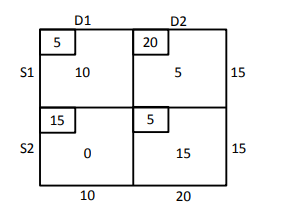
\includegraphics[width=0.75\columnwidth]{chapters/10/7/2/4/figs/fig.png}
 \end{center}
\caption{}
\label{fig:10/7/2/4Fig1}
\end{figure}
\fi

\item Find the position vector of the mid point of the vector joining the points $\vec{P}$(2, 3, 4)
and $\vec{Q}$(4, 1, –2).
\\
\solution
		\begin{enumerate}[label=\thesubsection.\arabic*,ref=\thesubsection.\theenumi]
\item Find the coordinates of the point which divides the join of $(-1,7) $ and $ (4,-3)$ in the ratio 2:3.
	\\
		\solution
	\input{chapters/10/7/2/1/section.tex}
\item Find the coordinates of the point $\vec{R}$ on the line segment joining the points $\vec{P}(-1,3)$ and $\vec{Q}(2,5)$ such that $PR=\frac{3}{5}PQ$.
\item Find the ratio in which the point $\vec{P}\brak{\frac{3}{4},\frac{5}{12}}$ divides the line segment joining the points $\vec{A}\brak{\frac{1}{2},\frac{3}{2}}$ and $ \vec{B}(2,-5)$.
\item Find the coordinates of the point which divides the line segment joining the points $(4,-3)$ and $(8,5)$ in the ratio $3:1$ internally.
\item Find the coordinates of the point $\vec{P}$ on $AD$ such that $AP : PD = 2 : 1$.
\item If the point $\vec{P} (2, 1)$ lies on the line segment joining points $\vec{A} (4, 2)$  and $ \vec{B} (8, 4)$,
then
\begin{enumerate}
	\item $AP =\frac{1}{3}{AB}$ 
\item ${AP}={PE}$
\item ${PB}=\frac{1}{3}{AB}$
\item${AP}=\frac{1}{2}{AB}$
 \end{enumerate}
\item Find the ratio in which the line segment joining the points $(-3,10)$  and  $(6,-8)$  is divided by $ (-1,6)$.
	\\
		\solution
	\input{chapters/10/7/2/4/section.tex}
\item Find the position vector of the mid point of the vector joining the points $\vec{P}$(2, 3, 4)
and $\vec{Q}$(4, 1, –2).
\\
\solution
		\input{chapters/12/10/2/16/section.tex}
\item Let $\vec{A}(4, 2), \vec{B}(6, 5)$  and $ \vec{C}(1, 4)$ be the vertices of $\triangle ABC$.
\begin{enumerate}
\item If $\vec{A}$ and  $\vec{B}$ are $(-2,-2)$ and  $(2,-4)$, respectively, find the coordinates of $\vec{P}$ such that $AP= \frac {3}{7}AB$  and $ \vec{P}$ lies on the line segment $AB$.
	\\
		\solution
	\input{chapters/10/7/2/8/section.tex}
\item Find the coordinates of the points which divide the line segment joining $A(-2,2)$  and  $\vec{B}(2,8)$ into four equal parts.
	\\
		\solution
	\input{chapters/10/7/2/9/section.tex}
\item In what ratio does the point $(-4,6)$ divide the line segment joining the points $\vec{A}(-6,0)$ and $\vec{B}(3,-8)$?
\item Given that $\vec{P}(3,2,-4), \vec{Q}(5,4,-6)$ and $\vec{R}(9,8,-10)$ are collinear. Find the ratio in which $\vec{Q}$ divides $PR$.
\item Points $\vec{A}(-6,10),\vec{B}(-4,6)$  and  $\vec{C}(3,-8)$ are collinear such that $AB=  \frac{2}{9}AC$.
\item The point which divides the line segment joining the points $\vec{P} (7, –6) $  and  $\vec{Q}(3, 4)$ in the 
ratio 1 : 2 internally lies in  which quadrant?
\item Find the coordinates of the points of trisection of the line segment joining $(4,-1)$  and  $(-2,3)$.
	\\
		\solution
	\input{chapters/10/7/2/2/section.tex}
\item Find the coordinates of the points which trisect the line segment joining the points $\vec{P}(4,2,-6)$ and $\vec{Q}(10,-16,6)$.
\item Find the coordinates of the points of trisection (i.e. points dividing to three equal parts) of the line segment joining the points $\vec{A}(2,-2)$ and $\vec{B}(-7,4)$.
\item Point $\vec{P}(5,-3)$ is one of the two points of trisection of line segment joining the points $\vec{A}(7,-2)$ and $\vec{B}(1,-5)$
\item Find the position vector of a point $\vec{R}$ which divides the line joining two points $\vec{P}$
and $\vec{Q}$ whose position vectors are $\hat{i}+2\hat{j}-\hat{k}$ and $-\hat{i}+\hat{j}+\hat{k}$ respectively, in the
ratio 2 : 1
\begin{enumerate}
    \item  internally
    \item  externally
\end{enumerate}
%\solution
%		\input{chapters/12/10/2/15/section.tex}
\item Find the coordinates of the point which divides the line segment joining the points which divides the line segment joining  the points $(-2,3,5)$ and $(1,-4,6)$ in the ratio 
\begin{enumerate}
\item $2:3$ internally,
\item $2:3$ externally
\end{enumerate}
\item Find the coordinates of the point which divides the line segment joining the points $(1,-2,3)$ and $(3,4,-5)$ in the ratio $2:3$
\begin{enumerate}
\item internally, and
\item externally
\end{enumerate}
\item Consider two points $\vec{P}$ and $\vec{Q}$ with position vectors $\overrightarrow{OP} = 3\overrightarrow{a}-2\overrightarrow{b}$ and $\overrightarrow{OQ}=\overrightarrow{a}+\overrightarrow{b}$. Find the position vector of a point $\vec{R}$ which divides the line joining $\vec{P}$ and $\vec{Q}$ in the ratio $2:1$, 
\begin{enumerate}
\item internally, and 
\item externally.
\end{enumerate}
\item The median from $\vec{A}$ meets $BC$ at $\vec{D}$. Find the coordinates of the point $\vec{D}$.
\item Find the coordinates of points $\vec{Q}$ and $\vec{R}$ on medians $BE$ and $CF$ respectively such that $BQ : QE = 2 : 1$  and  $CR : RF = 2 : 1$.
\item What do you observe?
\item If $\vec{A}, \vec{B}$ and $\vec{C}$  are the vertices of $\triangle ABC$, find the coordinates of the centroid of the triangle.
\end{enumerate}
\solution
	\input{chapters/10/7/4/7/section.tex}
\item If $\vec{P}(9a-2,-b)$ divides line segment joining $\vec{A}(3a+1,-3)$ and $\vec{B}(8a,5)$ in the ratio 3:1, find the values of $a$ and $b$.
\item Find the position vector of a point $\vec{R}$ which divides the line joining two points $\vec{P}$ and $\vec{Q}$ whose position vectors are $2\vec{a}+\vec{b}$ and $\vec{a}-3\vec{b}$ externally in the ratio $1:2$.
\item The position vector of the point which divides the join of points 2$\vec{a}$-3$\vec{b}$ $\text{and}$ $\vec{a}+\vec{b}$ in the ratio 3:1 is \rule{1cm}{0.1pt}.
\item If $\vec{a}$ and $\vec{b}$ are the postion vectors of $\vec{A}$ and $\vec{B}$, respectively, find the position vector of a point $\vec{C}$ in $BA$ produced such that $BC=1.5BA$.
\item Find the position vector of a point $\vec{R}$ which divides the line joining two points $\vec{P}$ and $\vec{Q}$ whose position vectors are $(2\vec{a}+\vec{b})$ and $(\vec{a}-3\vec{b})$
externally in the ratio 1 : 2. Also, show that $\vec{P}$ is the mid point of the line segment $RQ$.
\end{enumerate}

\item Let $\vec{A}(4, 2), \vec{B}(6, 5)$  and $ \vec{C}(1, 4)$ be the vertices of $\triangle ABC$.
\begin{enumerate}
\item If $\vec{A}$ and  $\vec{B}$ are $(-2,-2)$ and  $(2,-4)$, respectively, find the coordinates of $\vec{P}$ such that $AP= \frac {3}{7}AB$  and $ \vec{P}$ lies on the line segment $AB$.
	\\
		\solution
	\begin{enumerate}[label=\thesubsection.\arabic*,ref=\thesubsection.\theenumi]
\item Find the coordinates of the point which divides the join of $(-1,7) $ and $ (4,-3)$ in the ratio 2:3.
	\\
		\solution
	\input{chapters/10/7/2/1/section.tex}
\item Find the coordinates of the point $\vec{R}$ on the line segment joining the points $\vec{P}(-1,3)$ and $\vec{Q}(2,5)$ such that $PR=\frac{3}{5}PQ$.
\item Find the ratio in which the point $\vec{P}\brak{\frac{3}{4},\frac{5}{12}}$ divides the line segment joining the points $\vec{A}\brak{\frac{1}{2},\frac{3}{2}}$ and $ \vec{B}(2,-5)$.
\item Find the coordinates of the point which divides the line segment joining the points $(4,-3)$ and $(8,5)$ in the ratio $3:1$ internally.
\item Find the coordinates of the point $\vec{P}$ on $AD$ such that $AP : PD = 2 : 1$.
\item If the point $\vec{P} (2, 1)$ lies on the line segment joining points $\vec{A} (4, 2)$  and $ \vec{B} (8, 4)$,
then
\begin{enumerate}
	\item $AP =\frac{1}{3}{AB}$ 
\item ${AP}={PE}$
\item ${PB}=\frac{1}{3}{AB}$
\item${AP}=\frac{1}{2}{AB}$
 \end{enumerate}
\item Find the ratio in which the line segment joining the points $(-3,10)$  and  $(6,-8)$  is divided by $ (-1,6)$.
	\\
		\solution
	\input{chapters/10/7/2/4/section.tex}
\item Find the position vector of the mid point of the vector joining the points $\vec{P}$(2, 3, 4)
and $\vec{Q}$(4, 1, –2).
\\
\solution
		\input{chapters/12/10/2/16/section.tex}
\item Let $\vec{A}(4, 2), \vec{B}(6, 5)$  and $ \vec{C}(1, 4)$ be the vertices of $\triangle ABC$.
\begin{enumerate}
\item If $\vec{A}$ and  $\vec{B}$ are $(-2,-2)$ and  $(2,-4)$, respectively, find the coordinates of $\vec{P}$ such that $AP= \frac {3}{7}AB$  and $ \vec{P}$ lies on the line segment $AB$.
	\\
		\solution
	\input{chapters/10/7/2/8/section.tex}
\item Find the coordinates of the points which divide the line segment joining $A(-2,2)$  and  $\vec{B}(2,8)$ into four equal parts.
	\\
		\solution
	\input{chapters/10/7/2/9/section.tex}
\item In what ratio does the point $(-4,6)$ divide the line segment joining the points $\vec{A}(-6,0)$ and $\vec{B}(3,-8)$?
\item Given that $\vec{P}(3,2,-4), \vec{Q}(5,4,-6)$ and $\vec{R}(9,8,-10)$ are collinear. Find the ratio in which $\vec{Q}$ divides $PR$.
\item Points $\vec{A}(-6,10),\vec{B}(-4,6)$  and  $\vec{C}(3,-8)$ are collinear such that $AB=  \frac{2}{9}AC$.
\item The point which divides the line segment joining the points $\vec{P} (7, –6) $  and  $\vec{Q}(3, 4)$ in the 
ratio 1 : 2 internally lies in  which quadrant?
\item Find the coordinates of the points of trisection of the line segment joining $(4,-1)$  and  $(-2,3)$.
	\\
		\solution
	\input{chapters/10/7/2/2/section.tex}
\item Find the coordinates of the points which trisect the line segment joining the points $\vec{P}(4,2,-6)$ and $\vec{Q}(10,-16,6)$.
\item Find the coordinates of the points of trisection (i.e. points dividing to three equal parts) of the line segment joining the points $\vec{A}(2,-2)$ and $\vec{B}(-7,4)$.
\item Point $\vec{P}(5,-3)$ is one of the two points of trisection of line segment joining the points $\vec{A}(7,-2)$ and $\vec{B}(1,-5)$
\item Find the position vector of a point $\vec{R}$ which divides the line joining two points $\vec{P}$
and $\vec{Q}$ whose position vectors are $\hat{i}+2\hat{j}-\hat{k}$ and $-\hat{i}+\hat{j}+\hat{k}$ respectively, in the
ratio 2 : 1
\begin{enumerate}
    \item  internally
    \item  externally
\end{enumerate}
%\solution
%		\input{chapters/12/10/2/15/section.tex}
\item Find the coordinates of the point which divides the line segment joining the points which divides the line segment joining  the points $(-2,3,5)$ and $(1,-4,6)$ in the ratio 
\begin{enumerate}
\item $2:3$ internally,
\item $2:3$ externally
\end{enumerate}
\item Find the coordinates of the point which divides the line segment joining the points $(1,-2,3)$ and $(3,4,-5)$ in the ratio $2:3$
\begin{enumerate}
\item internally, and
\item externally
\end{enumerate}
\item Consider two points $\vec{P}$ and $\vec{Q}$ with position vectors $\overrightarrow{OP} = 3\overrightarrow{a}-2\overrightarrow{b}$ and $\overrightarrow{OQ}=\overrightarrow{a}+\overrightarrow{b}$. Find the position vector of a point $\vec{R}$ which divides the line joining $\vec{P}$ and $\vec{Q}$ in the ratio $2:1$, 
\begin{enumerate}
\item internally, and 
\item externally.
\end{enumerate}
\item The median from $\vec{A}$ meets $BC$ at $\vec{D}$. Find the coordinates of the point $\vec{D}$.
\item Find the coordinates of points $\vec{Q}$ and $\vec{R}$ on medians $BE$ and $CF$ respectively such that $BQ : QE = 2 : 1$  and  $CR : RF = 2 : 1$.
\item What do you observe?
\item If $\vec{A}, \vec{B}$ and $\vec{C}$  are the vertices of $\triangle ABC$, find the coordinates of the centroid of the triangle.
\end{enumerate}
\solution
	\input{chapters/10/7/4/7/section.tex}
\item If $\vec{P}(9a-2,-b)$ divides line segment joining $\vec{A}(3a+1,-3)$ and $\vec{B}(8a,5)$ in the ratio 3:1, find the values of $a$ and $b$.
\item Find the position vector of a point $\vec{R}$ which divides the line joining two points $\vec{P}$ and $\vec{Q}$ whose position vectors are $2\vec{a}+\vec{b}$ and $\vec{a}-3\vec{b}$ externally in the ratio $1:2$.
\item The position vector of the point which divides the join of points 2$\vec{a}$-3$\vec{b}$ $\text{and}$ $\vec{a}+\vec{b}$ in the ratio 3:1 is \rule{1cm}{0.1pt}.
\item If $\vec{a}$ and $\vec{b}$ are the postion vectors of $\vec{A}$ and $\vec{B}$, respectively, find the position vector of a point $\vec{C}$ in $BA$ produced such that $BC=1.5BA$.
\item Find the position vector of a point $\vec{R}$ which divides the line joining two points $\vec{P}$ and $\vec{Q}$ whose position vectors are $(2\vec{a}+\vec{b})$ and $(\vec{a}-3\vec{b})$
externally in the ratio 1 : 2. Also, show that $\vec{P}$ is the mid point of the line segment $RQ$.
\end{enumerate}

\item Find the coordinates of the points which divide the line segment joining $A(-2,2)$  and  $\vec{B}(2,8)$ into four equal parts.
	\\
		\solution
	\begin{enumerate}[label=\thesubsection.\arabic*,ref=\thesubsection.\theenumi]
\item Find the coordinates of the point which divides the join of $(-1,7) $ and $ (4,-3)$ in the ratio 2:3.
	\\
		\solution
	\input{chapters/10/7/2/1/section.tex}
\item Find the coordinates of the point $\vec{R}$ on the line segment joining the points $\vec{P}(-1,3)$ and $\vec{Q}(2,5)$ such that $PR=\frac{3}{5}PQ$.
\item Find the ratio in which the point $\vec{P}\brak{\frac{3}{4},\frac{5}{12}}$ divides the line segment joining the points $\vec{A}\brak{\frac{1}{2},\frac{3}{2}}$ and $ \vec{B}(2,-5)$.
\item Find the coordinates of the point which divides the line segment joining the points $(4,-3)$ and $(8,5)$ in the ratio $3:1$ internally.
\item Find the coordinates of the point $\vec{P}$ on $AD$ such that $AP : PD = 2 : 1$.
\item If the point $\vec{P} (2, 1)$ lies on the line segment joining points $\vec{A} (4, 2)$  and $ \vec{B} (8, 4)$,
then
\begin{enumerate}
	\item $AP =\frac{1}{3}{AB}$ 
\item ${AP}={PE}$
\item ${PB}=\frac{1}{3}{AB}$
\item${AP}=\frac{1}{2}{AB}$
 \end{enumerate}
\item Find the ratio in which the line segment joining the points $(-3,10)$  and  $(6,-8)$  is divided by $ (-1,6)$.
	\\
		\solution
	\input{chapters/10/7/2/4/section.tex}
\item Find the position vector of the mid point of the vector joining the points $\vec{P}$(2, 3, 4)
and $\vec{Q}$(4, 1, –2).
\\
\solution
		\input{chapters/12/10/2/16/section.tex}
\item Let $\vec{A}(4, 2), \vec{B}(6, 5)$  and $ \vec{C}(1, 4)$ be the vertices of $\triangle ABC$.
\begin{enumerate}
\item If $\vec{A}$ and  $\vec{B}$ are $(-2,-2)$ and  $(2,-4)$, respectively, find the coordinates of $\vec{P}$ such that $AP= \frac {3}{7}AB$  and $ \vec{P}$ lies on the line segment $AB$.
	\\
		\solution
	\input{chapters/10/7/2/8/section.tex}
\item Find the coordinates of the points which divide the line segment joining $A(-2,2)$  and  $\vec{B}(2,8)$ into four equal parts.
	\\
		\solution
	\input{chapters/10/7/2/9/section.tex}
\item In what ratio does the point $(-4,6)$ divide the line segment joining the points $\vec{A}(-6,0)$ and $\vec{B}(3,-8)$?
\item Given that $\vec{P}(3,2,-4), \vec{Q}(5,4,-6)$ and $\vec{R}(9,8,-10)$ are collinear. Find the ratio in which $\vec{Q}$ divides $PR$.
\item Points $\vec{A}(-6,10),\vec{B}(-4,6)$  and  $\vec{C}(3,-8)$ are collinear such that $AB=  \frac{2}{9}AC$.
\item The point which divides the line segment joining the points $\vec{P} (7, –6) $  and  $\vec{Q}(3, 4)$ in the 
ratio 1 : 2 internally lies in  which quadrant?
\item Find the coordinates of the points of trisection of the line segment joining $(4,-1)$  and  $(-2,3)$.
	\\
		\solution
	\input{chapters/10/7/2/2/section.tex}
\item Find the coordinates of the points which trisect the line segment joining the points $\vec{P}(4,2,-6)$ and $\vec{Q}(10,-16,6)$.
\item Find the coordinates of the points of trisection (i.e. points dividing to three equal parts) of the line segment joining the points $\vec{A}(2,-2)$ and $\vec{B}(-7,4)$.
\item Point $\vec{P}(5,-3)$ is one of the two points of trisection of line segment joining the points $\vec{A}(7,-2)$ and $\vec{B}(1,-5)$
\item Find the position vector of a point $\vec{R}$ which divides the line joining two points $\vec{P}$
and $\vec{Q}$ whose position vectors are $\hat{i}+2\hat{j}-\hat{k}$ and $-\hat{i}+\hat{j}+\hat{k}$ respectively, in the
ratio 2 : 1
\begin{enumerate}
    \item  internally
    \item  externally
\end{enumerate}
%\solution
%		\input{chapters/12/10/2/15/section.tex}
\item Find the coordinates of the point which divides the line segment joining the points which divides the line segment joining  the points $(-2,3,5)$ and $(1,-4,6)$ in the ratio 
\begin{enumerate}
\item $2:3$ internally,
\item $2:3$ externally
\end{enumerate}
\item Find the coordinates of the point which divides the line segment joining the points $(1,-2,3)$ and $(3,4,-5)$ in the ratio $2:3$
\begin{enumerate}
\item internally, and
\item externally
\end{enumerate}
\item Consider two points $\vec{P}$ and $\vec{Q}$ with position vectors $\overrightarrow{OP} = 3\overrightarrow{a}-2\overrightarrow{b}$ and $\overrightarrow{OQ}=\overrightarrow{a}+\overrightarrow{b}$. Find the position vector of a point $\vec{R}$ which divides the line joining $\vec{P}$ and $\vec{Q}$ in the ratio $2:1$, 
\begin{enumerate}
\item internally, and 
\item externally.
\end{enumerate}
\item The median from $\vec{A}$ meets $BC$ at $\vec{D}$. Find the coordinates of the point $\vec{D}$.
\item Find the coordinates of points $\vec{Q}$ and $\vec{R}$ on medians $BE$ and $CF$ respectively such that $BQ : QE = 2 : 1$  and  $CR : RF = 2 : 1$.
\item What do you observe?
\item If $\vec{A}, \vec{B}$ and $\vec{C}$  are the vertices of $\triangle ABC$, find the coordinates of the centroid of the triangle.
\end{enumerate}
\solution
	\input{chapters/10/7/4/7/section.tex}
\item If $\vec{P}(9a-2,-b)$ divides line segment joining $\vec{A}(3a+1,-3)$ and $\vec{B}(8a,5)$ in the ratio 3:1, find the values of $a$ and $b$.
\item Find the position vector of a point $\vec{R}$ which divides the line joining two points $\vec{P}$ and $\vec{Q}$ whose position vectors are $2\vec{a}+\vec{b}$ and $\vec{a}-3\vec{b}$ externally in the ratio $1:2$.
\item The position vector of the point which divides the join of points 2$\vec{a}$-3$\vec{b}$ $\text{and}$ $\vec{a}+\vec{b}$ in the ratio 3:1 is \rule{1cm}{0.1pt}.
\item If $\vec{a}$ and $\vec{b}$ are the postion vectors of $\vec{A}$ and $\vec{B}$, respectively, find the position vector of a point $\vec{C}$ in $BA$ produced such that $BC=1.5BA$.
\item Find the position vector of a point $\vec{R}$ which divides the line joining two points $\vec{P}$ and $\vec{Q}$ whose position vectors are $(2\vec{a}+\vec{b})$ and $(\vec{a}-3\vec{b})$
externally in the ratio 1 : 2. Also, show that $\vec{P}$ is the mid point of the line segment $RQ$.
\end{enumerate}

\item In what ratio does the point $(-4,6)$ divide the line segment joining the points $\vec{A}(-6,0)$ and $\vec{B}(3,-8)$?
\item Given that $\vec{P}(3,2,-4), \vec{Q}(5,4,-6)$ and $\vec{R}(9,8,-10)$ are collinear. Find the ratio in which $\vec{Q}$ divides $PR$.
\item Points $\vec{A}(-6,10),\vec{B}(-4,6)$  and  $\vec{C}(3,-8)$ are collinear such that $AB=  \frac{2}{9}AC$.
\item The point which divides the line segment joining the points $\vec{P} (7, –6) $  and  $\vec{Q}(3, 4)$ in the 
ratio 1 : 2 internally lies in  which quadrant?
\item Find the coordinates of the points of trisection of the line segment joining $(4,-1)$  and  $(-2,3)$.
	\\
		\solution
	Using section formula,
\begin{align}
\vec{R}=\frac{1}{1+\frac{1}{2}}\brak{\myvec{4\\-1}+\frac{1}{2}\myvec{-2\\3}}
=\myvec{2\\ \frac{1}{3}}\\
\vec{S}=\frac{1}{1+\frac{2}{1}}\brak{\myvec{4\\-1}+\frac{2}{1}\myvec{-2\\3}}
=\myvec{0\\ \frac{5}{3}}
\end{align}
which are the desired points of trisection.
\iffalse
See
		\figref{fig:chapters/10/7/2/2/Figure}
\begin{figure}[H]
\centering
\includegraphics[width=0.75\columnwidth]{chapters/10/7/2/2/figs/dj.pdf}
\caption{}
		\label{fig:chapters/10/7/2/2/Figure}
\end{figure}
\fi

\item Find the coordinates of the points which trisect the line segment joining the points $\vec{P}(4,2,-6)$ and $\vec{Q}(10,-16,6)$.
\item Find the coordinates of the points of trisection (i.e. points dividing to three equal parts) of the line segment joining the points $\vec{A}(2,-2)$ and $\vec{B}(-7,4)$.
\item Point $\vec{P}(5,-3)$ is one of the two points of trisection of line segment joining the points $\vec{A}(7,-2)$ and $\vec{B}(1,-5)$
\item Find the position vector of a point $\vec{R}$ which divides the line joining two points $\vec{P}$
and $\vec{Q}$ whose position vectors are $\hat{i}+2\hat{j}-\hat{k}$ and $-\hat{i}+\hat{j}+\hat{k}$ respectively, in the
ratio 2 : 1
\begin{enumerate}
    \item  internally
    \item  externally
\end{enumerate}
%\solution
%		\begin{enumerate}[label=\thesubsection.\arabic*,ref=\thesubsection.\theenumi]
\item Find the coordinates of the point which divides the join of $(-1,7) $ and $ (4,-3)$ in the ratio 2:3.
	\\
		\solution
	\input{chapters/10/7/2/1/section.tex}
\item Find the coordinates of the point $\vec{R}$ on the line segment joining the points $\vec{P}(-1,3)$ and $\vec{Q}(2,5)$ such that $PR=\frac{3}{5}PQ$.
\item Find the ratio in which the point $\vec{P}\brak{\frac{3}{4},\frac{5}{12}}$ divides the line segment joining the points $\vec{A}\brak{\frac{1}{2},\frac{3}{2}}$ and $ \vec{B}(2,-5)$.
\item Find the coordinates of the point which divides the line segment joining the points $(4,-3)$ and $(8,5)$ in the ratio $3:1$ internally.
\item Find the coordinates of the point $\vec{P}$ on $AD$ such that $AP : PD = 2 : 1$.
\item If the point $\vec{P} (2, 1)$ lies on the line segment joining points $\vec{A} (4, 2)$  and $ \vec{B} (8, 4)$,
then
\begin{enumerate}
	\item $AP =\frac{1}{3}{AB}$ 
\item ${AP}={PE}$
\item ${PB}=\frac{1}{3}{AB}$
\item${AP}=\frac{1}{2}{AB}$
 \end{enumerate}
\item Find the ratio in which the line segment joining the points $(-3,10)$  and  $(6,-8)$  is divided by $ (-1,6)$.
	\\
		\solution
	\input{chapters/10/7/2/4/section.tex}
\item Find the position vector of the mid point of the vector joining the points $\vec{P}$(2, 3, 4)
and $\vec{Q}$(4, 1, –2).
\\
\solution
		\input{chapters/12/10/2/16/section.tex}
\item Let $\vec{A}(4, 2), \vec{B}(6, 5)$  and $ \vec{C}(1, 4)$ be the vertices of $\triangle ABC$.
\begin{enumerate}
\item If $\vec{A}$ and  $\vec{B}$ are $(-2,-2)$ and  $(2,-4)$, respectively, find the coordinates of $\vec{P}$ such that $AP= \frac {3}{7}AB$  and $ \vec{P}$ lies on the line segment $AB$.
	\\
		\solution
	\input{chapters/10/7/2/8/section.tex}
\item Find the coordinates of the points which divide the line segment joining $A(-2,2)$  and  $\vec{B}(2,8)$ into four equal parts.
	\\
		\solution
	\input{chapters/10/7/2/9/section.tex}
\item In what ratio does the point $(-4,6)$ divide the line segment joining the points $\vec{A}(-6,0)$ and $\vec{B}(3,-8)$?
\item Given that $\vec{P}(3,2,-4), \vec{Q}(5,4,-6)$ and $\vec{R}(9,8,-10)$ are collinear. Find the ratio in which $\vec{Q}$ divides $PR$.
\item Points $\vec{A}(-6,10),\vec{B}(-4,6)$  and  $\vec{C}(3,-8)$ are collinear such that $AB=  \frac{2}{9}AC$.
\item The point which divides the line segment joining the points $\vec{P} (7, –6) $  and  $\vec{Q}(3, 4)$ in the 
ratio 1 : 2 internally lies in  which quadrant?
\item Find the coordinates of the points of trisection of the line segment joining $(4,-1)$  and  $(-2,3)$.
	\\
		\solution
	\input{chapters/10/7/2/2/section.tex}
\item Find the coordinates of the points which trisect the line segment joining the points $\vec{P}(4,2,-6)$ and $\vec{Q}(10,-16,6)$.
\item Find the coordinates of the points of trisection (i.e. points dividing to three equal parts) of the line segment joining the points $\vec{A}(2,-2)$ and $\vec{B}(-7,4)$.
\item Point $\vec{P}(5,-3)$ is one of the two points of trisection of line segment joining the points $\vec{A}(7,-2)$ and $\vec{B}(1,-5)$
\item Find the position vector of a point $\vec{R}$ which divides the line joining two points $\vec{P}$
and $\vec{Q}$ whose position vectors are $\hat{i}+2\hat{j}-\hat{k}$ and $-\hat{i}+\hat{j}+\hat{k}$ respectively, in the
ratio 2 : 1
\begin{enumerate}
    \item  internally
    \item  externally
\end{enumerate}
%\solution
%		\input{chapters/12/10/2/15/section.tex}
\item Find the coordinates of the point which divides the line segment joining the points which divides the line segment joining  the points $(-2,3,5)$ and $(1,-4,6)$ in the ratio 
\begin{enumerate}
\item $2:3$ internally,
\item $2:3$ externally
\end{enumerate}
\item Find the coordinates of the point which divides the line segment joining the points $(1,-2,3)$ and $(3,4,-5)$ in the ratio $2:3$
\begin{enumerate}
\item internally, and
\item externally
\end{enumerate}
\item Consider two points $\vec{P}$ and $\vec{Q}$ with position vectors $\overrightarrow{OP} = 3\overrightarrow{a}-2\overrightarrow{b}$ and $\overrightarrow{OQ}=\overrightarrow{a}+\overrightarrow{b}$. Find the position vector of a point $\vec{R}$ which divides the line joining $\vec{P}$ and $\vec{Q}$ in the ratio $2:1$, 
\begin{enumerate}
\item internally, and 
\item externally.
\end{enumerate}
\item The median from $\vec{A}$ meets $BC$ at $\vec{D}$. Find the coordinates of the point $\vec{D}$.
\item Find the coordinates of points $\vec{Q}$ and $\vec{R}$ on medians $BE$ and $CF$ respectively such that $BQ : QE = 2 : 1$  and  $CR : RF = 2 : 1$.
\item What do you observe?
\item If $\vec{A}, \vec{B}$ and $\vec{C}$  are the vertices of $\triangle ABC$, find the coordinates of the centroid of the triangle.
\end{enumerate}
\solution
	\input{chapters/10/7/4/7/section.tex}
\item If $\vec{P}(9a-2,-b)$ divides line segment joining $\vec{A}(3a+1,-3)$ and $\vec{B}(8a,5)$ in the ratio 3:1, find the values of $a$ and $b$.
\item Find the position vector of a point $\vec{R}$ which divides the line joining two points $\vec{P}$ and $\vec{Q}$ whose position vectors are $2\vec{a}+\vec{b}$ and $\vec{a}-3\vec{b}$ externally in the ratio $1:2$.
\item The position vector of the point which divides the join of points 2$\vec{a}$-3$\vec{b}$ $\text{and}$ $\vec{a}+\vec{b}$ in the ratio 3:1 is \rule{1cm}{0.1pt}.
\item If $\vec{a}$ and $\vec{b}$ are the postion vectors of $\vec{A}$ and $\vec{B}$, respectively, find the position vector of a point $\vec{C}$ in $BA$ produced such that $BC=1.5BA$.
\item Find the position vector of a point $\vec{R}$ which divides the line joining two points $\vec{P}$ and $\vec{Q}$ whose position vectors are $(2\vec{a}+\vec{b})$ and $(\vec{a}-3\vec{b})$
externally in the ratio 1 : 2. Also, show that $\vec{P}$ is the mid point of the line segment $RQ$.
\end{enumerate}

\item Find the coordinates of the point which divides the line segment joining the points which divides the line segment joining  the points $(-2,3,5)$ and $(1,-4,6)$ in the ratio 
\begin{enumerate}
\item $2:3$ internally,
\item $2:3$ externally
\end{enumerate}
\item Find the coordinates of the point which divides the line segment joining the points $(1,-2,3)$ and $(3,4,-5)$ in the ratio $2:3$
\begin{enumerate}
\item internally, and
\item externally
\end{enumerate}
\item Consider two points $\vec{P}$ and $\vec{Q}$ with position vectors $\overrightarrow{OP} = 3\overrightarrow{a}-2\overrightarrow{b}$ and $\overrightarrow{OQ}=\overrightarrow{a}+\overrightarrow{b}$. Find the position vector of a point $\vec{R}$ which divides the line joining $\vec{P}$ and $\vec{Q}$ in the ratio $2:1$, 
\begin{enumerate}
\item internally, and 
\item externally.
\end{enumerate}
\item The median from $\vec{A}$ meets $BC$ at $\vec{D}$. Find the coordinates of the point $\vec{D}$.
\item Find the coordinates of points $\vec{Q}$ and $\vec{R}$ on medians $BE$ and $CF$ respectively such that $BQ : QE = 2 : 1$  and  $CR : RF = 2 : 1$.
\item What do you observe?
\item If $\vec{A}, \vec{B}$ and $\vec{C}$  are the vertices of $\triangle ABC$, find the coordinates of the centroid of the triangle.
\end{enumerate}
\solution
	\begin{enumerate}[label=\thesubsection.\arabic*,ref=\thesubsection.\theenumi]
\item Find the coordinates of the point which divides the join of $(-1,7) $ and $ (4,-3)$ in the ratio 2:3.
	\\
		\solution
	\input{chapters/10/7/2/1/section.tex}
\item Find the coordinates of the point $\vec{R}$ on the line segment joining the points $\vec{P}(-1,3)$ and $\vec{Q}(2,5)$ such that $PR=\frac{3}{5}PQ$.
\item Find the ratio in which the point $\vec{P}\brak{\frac{3}{4},\frac{5}{12}}$ divides the line segment joining the points $\vec{A}\brak{\frac{1}{2},\frac{3}{2}}$ and $ \vec{B}(2,-5)$.
\item Find the coordinates of the point which divides the line segment joining the points $(4,-3)$ and $(8,5)$ in the ratio $3:1$ internally.
\item Find the coordinates of the point $\vec{P}$ on $AD$ such that $AP : PD = 2 : 1$.
\item If the point $\vec{P} (2, 1)$ lies on the line segment joining points $\vec{A} (4, 2)$  and $ \vec{B} (8, 4)$,
then
\begin{enumerate}
	\item $AP =\frac{1}{3}{AB}$ 
\item ${AP}={PE}$
\item ${PB}=\frac{1}{3}{AB}$
\item${AP}=\frac{1}{2}{AB}$
 \end{enumerate}
\item Find the ratio in which the line segment joining the points $(-3,10)$  and  $(6,-8)$  is divided by $ (-1,6)$.
	\\
		\solution
	\input{chapters/10/7/2/4/section.tex}
\item Find the position vector of the mid point of the vector joining the points $\vec{P}$(2, 3, 4)
and $\vec{Q}$(4, 1, –2).
\\
\solution
		\input{chapters/12/10/2/16/section.tex}
\item Let $\vec{A}(4, 2), \vec{B}(6, 5)$  and $ \vec{C}(1, 4)$ be the vertices of $\triangle ABC$.
\begin{enumerate}
\item If $\vec{A}$ and  $\vec{B}$ are $(-2,-2)$ and  $(2,-4)$, respectively, find the coordinates of $\vec{P}$ such that $AP= \frac {3}{7}AB$  and $ \vec{P}$ lies on the line segment $AB$.
	\\
		\solution
	\input{chapters/10/7/2/8/section.tex}
\item Find the coordinates of the points which divide the line segment joining $A(-2,2)$  and  $\vec{B}(2,8)$ into four equal parts.
	\\
		\solution
	\input{chapters/10/7/2/9/section.tex}
\item In what ratio does the point $(-4,6)$ divide the line segment joining the points $\vec{A}(-6,0)$ and $\vec{B}(3,-8)$?
\item Given that $\vec{P}(3,2,-4), \vec{Q}(5,4,-6)$ and $\vec{R}(9,8,-10)$ are collinear. Find the ratio in which $\vec{Q}$ divides $PR$.
\item Points $\vec{A}(-6,10),\vec{B}(-4,6)$  and  $\vec{C}(3,-8)$ are collinear such that $AB=  \frac{2}{9}AC$.
\item The point which divides the line segment joining the points $\vec{P} (7, –6) $  and  $\vec{Q}(3, 4)$ in the 
ratio 1 : 2 internally lies in  which quadrant?
\item Find the coordinates of the points of trisection of the line segment joining $(4,-1)$  and  $(-2,3)$.
	\\
		\solution
	\input{chapters/10/7/2/2/section.tex}
\item Find the coordinates of the points which trisect the line segment joining the points $\vec{P}(4,2,-6)$ and $\vec{Q}(10,-16,6)$.
\item Find the coordinates of the points of trisection (i.e. points dividing to three equal parts) of the line segment joining the points $\vec{A}(2,-2)$ and $\vec{B}(-7,4)$.
\item Point $\vec{P}(5,-3)$ is one of the two points of trisection of line segment joining the points $\vec{A}(7,-2)$ and $\vec{B}(1,-5)$
\item Find the position vector of a point $\vec{R}$ which divides the line joining two points $\vec{P}$
and $\vec{Q}$ whose position vectors are $\hat{i}+2\hat{j}-\hat{k}$ and $-\hat{i}+\hat{j}+\hat{k}$ respectively, in the
ratio 2 : 1
\begin{enumerate}
    \item  internally
    \item  externally
\end{enumerate}
%\solution
%		\input{chapters/12/10/2/15/section.tex}
\item Find the coordinates of the point which divides the line segment joining the points which divides the line segment joining  the points $(-2,3,5)$ and $(1,-4,6)$ in the ratio 
\begin{enumerate}
\item $2:3$ internally,
\item $2:3$ externally
\end{enumerate}
\item Find the coordinates of the point which divides the line segment joining the points $(1,-2,3)$ and $(3,4,-5)$ in the ratio $2:3$
\begin{enumerate}
\item internally, and
\item externally
\end{enumerate}
\item Consider two points $\vec{P}$ and $\vec{Q}$ with position vectors $\overrightarrow{OP} = 3\overrightarrow{a}-2\overrightarrow{b}$ and $\overrightarrow{OQ}=\overrightarrow{a}+\overrightarrow{b}$. Find the position vector of a point $\vec{R}$ which divides the line joining $\vec{P}$ and $\vec{Q}$ in the ratio $2:1$, 
\begin{enumerate}
\item internally, and 
\item externally.
\end{enumerate}
\item The median from $\vec{A}$ meets $BC$ at $\vec{D}$. Find the coordinates of the point $\vec{D}$.
\item Find the coordinates of points $\vec{Q}$ and $\vec{R}$ on medians $BE$ and $CF$ respectively such that $BQ : QE = 2 : 1$  and  $CR : RF = 2 : 1$.
\item What do you observe?
\item If $\vec{A}, \vec{B}$ and $\vec{C}$  are the vertices of $\triangle ABC$, find the coordinates of the centroid of the triangle.
\end{enumerate}
\solution
	\input{chapters/10/7/4/7/section.tex}
\item If $\vec{P}(9a-2,-b)$ divides line segment joining $\vec{A}(3a+1,-3)$ and $\vec{B}(8a,5)$ in the ratio 3:1, find the values of $a$ and $b$.
\item Find the position vector of a point $\vec{R}$ which divides the line joining two points $\vec{P}$ and $\vec{Q}$ whose position vectors are $2\vec{a}+\vec{b}$ and $\vec{a}-3\vec{b}$ externally in the ratio $1:2$.
\item The position vector of the point which divides the join of points 2$\vec{a}$-3$\vec{b}$ $\text{and}$ $\vec{a}+\vec{b}$ in the ratio 3:1 is \rule{1cm}{0.1pt}.
\item If $\vec{a}$ and $\vec{b}$ are the postion vectors of $\vec{A}$ and $\vec{B}$, respectively, find the position vector of a point $\vec{C}$ in $BA$ produced such that $BC=1.5BA$.
\item Find the position vector of a point $\vec{R}$ which divides the line joining two points $\vec{P}$ and $\vec{Q}$ whose position vectors are $(2\vec{a}+\vec{b})$ and $(\vec{a}-3\vec{b})$
externally in the ratio 1 : 2. Also, show that $\vec{P}$ is the mid point of the line segment $RQ$.
\end{enumerate}

\item If $\vec{P}(9a-2,-b)$ divides line segment joining $\vec{A}(3a+1,-3)$ and $\vec{B}(8a,5)$ in the ratio 3:1, find the values of $a$ and $b$.
\item Find the position vector of a point $\vec{R}$ which divides the line joining two points $\vec{P}$ and $\vec{Q}$ whose position vectors are $2\vec{a}+\vec{b}$ and $\vec{a}-3\vec{b}$ externally in the ratio $1:2$.
\item The position vector of the point which divides the join of points 2$\vec{a}$-3$\vec{b}$ $\text{and}$ $\vec{a}+\vec{b}$ in the ratio 3:1 is \rule{1cm}{0.1pt}.
\item If $\vec{a}$ and $\vec{b}$ are the postion vectors of $\vec{A}$ and $\vec{B}$, respectively, find the position vector of a point $\vec{C}$ in $BA$ produced such that $BC=1.5BA$.
\item Find the position vector of a point $\vec{R}$ which divides the line joining two points $\vec{P}$ and $\vec{Q}$ whose position vectors are $(2\vec{a}+\vec{b})$ and $(\vec{a}-3\vec{b})$
externally in the ratio 1 : 2. Also, show that $\vec{P}$ is the mid point of the line segment $RQ$.
\end{enumerate}

\item In what ratio does the point $(-4,6)$ divide the line segment joining the points $\vec{A}(-6,0)$ and $\vec{B}(3,-8)$?
\item Given that $\vec{P}(3,2,-4), \vec{Q}(5,4,-6)$ and $\vec{R}(9,8,-10)$ are collinear. Find the ratio in which $\vec{Q}$ divides $PR$.
\item Points $\vec{A}(-6,10),\vec{B}(-4,6)$  and  $\vec{C}(3,-8)$ are collinear such that $AB=  \frac{2}{9}AC$.
\item The point which divides the line segment joining the points $\vec{P} (7, –6) $  and  $\vec{Q}(3, 4)$ in the 
ratio 1 : 2 internally lies in  which quadrant?
\item Find the coordinates of the points of trisection of the line segment joining $(4,-1)$  and  $(-2,3)$.
	\\
		\solution
	Using section formula,
\begin{align}
\vec{R}=\frac{1}{1+\frac{1}{2}}\brak{\myvec{4\\-1}+\frac{1}{2}\myvec{-2\\3}}
=\myvec{2\\ \frac{1}{3}}\\
\vec{S}=\frac{1}{1+\frac{2}{1}}\brak{\myvec{4\\-1}+\frac{2}{1}\myvec{-2\\3}}
=\myvec{0\\ \frac{5}{3}}
\end{align}
which are the desired points of trisection.
\iffalse
See
		\figref{fig:chapters/10/7/2/2/Figure}
\begin{figure}[H]
\centering
\includegraphics[width=0.75\columnwidth]{chapters/10/7/2/2/figs/dj.pdf}
\caption{}
		\label{fig:chapters/10/7/2/2/Figure}
\end{figure}
\fi

\item Find the coordinates of the points which trisect the line segment joining the points $\vec{P}(4,2,-6)$ and $\vec{Q}(10,-16,6)$.
\item Find the coordinates of the points of trisection (i.e. points dividing to three equal parts) of the line segment joining the points $\vec{A}(2,-2)$ and $\vec{B}(-7,4)$.
\item Point $\vec{P}(5,-3)$ is one of the two points of trisection of line segment joining the points $\vec{A}(7,-2)$ and $\vec{B}(1,-5)$
\item Find the position vector of a point $\vec{R}$ which divides the line joining two points $\vec{P}$
and $\vec{Q}$ whose position vectors are $\hat{i}+2\hat{j}-\hat{k}$ and $-\hat{i}+\hat{j}+\hat{k}$ respectively, in the
ratio 2 : 1
\begin{enumerate}
    \item  internally
    \item  externally
\end{enumerate}
%\solution
%		\begin{enumerate}[label=\thesubsection.\arabic*,ref=\thesubsection.\theenumi]
\item Find the coordinates of the point which divides the join of $(-1,7) $ and $ (4,-3)$ in the ratio 2:3.
	\\
		\solution
	\begin{enumerate}[label=\thesubsection.\arabic*,ref=\thesubsection.\theenumi]
\item Find the coordinates of the point which divides the join of $(-1,7) $ and $ (4,-3)$ in the ratio 2:3.
	\\
		\solution
	\input{chapters/10/7/2/1/section.tex}
\item Find the coordinates of the point $\vec{R}$ on the line segment joining the points $\vec{P}(-1,3)$ and $\vec{Q}(2,5)$ such that $PR=\frac{3}{5}PQ$.
\item Find the ratio in which the point $\vec{P}\brak{\frac{3}{4},\frac{5}{12}}$ divides the line segment joining the points $\vec{A}\brak{\frac{1}{2},\frac{3}{2}}$ and $ \vec{B}(2,-5)$.
\item Find the coordinates of the point which divides the line segment joining the points $(4,-3)$ and $(8,5)$ in the ratio $3:1$ internally.
\item Find the coordinates of the point $\vec{P}$ on $AD$ such that $AP : PD = 2 : 1$.
\item If the point $\vec{P} (2, 1)$ lies on the line segment joining points $\vec{A} (4, 2)$  and $ \vec{B} (8, 4)$,
then
\begin{enumerate}
	\item $AP =\frac{1}{3}{AB}$ 
\item ${AP}={PE}$
\item ${PB}=\frac{1}{3}{AB}$
\item${AP}=\frac{1}{2}{AB}$
 \end{enumerate}
\item Find the ratio in which the line segment joining the points $(-3,10)$  and  $(6,-8)$  is divided by $ (-1,6)$.
	\\
		\solution
	\input{chapters/10/7/2/4/section.tex}
\item Find the position vector of the mid point of the vector joining the points $\vec{P}$(2, 3, 4)
and $\vec{Q}$(4, 1, –2).
\\
\solution
		\input{chapters/12/10/2/16/section.tex}
\item Let $\vec{A}(4, 2), \vec{B}(6, 5)$  and $ \vec{C}(1, 4)$ be the vertices of $\triangle ABC$.
\begin{enumerate}
\item If $\vec{A}$ and  $\vec{B}$ are $(-2,-2)$ and  $(2,-4)$, respectively, find the coordinates of $\vec{P}$ such that $AP= \frac {3}{7}AB$  and $ \vec{P}$ lies on the line segment $AB$.
	\\
		\solution
	\input{chapters/10/7/2/8/section.tex}
\item Find the coordinates of the points which divide the line segment joining $A(-2,2)$  and  $\vec{B}(2,8)$ into four equal parts.
	\\
		\solution
	\input{chapters/10/7/2/9/section.tex}
\item In what ratio does the point $(-4,6)$ divide the line segment joining the points $\vec{A}(-6,0)$ and $\vec{B}(3,-8)$?
\item Given that $\vec{P}(3,2,-4), \vec{Q}(5,4,-6)$ and $\vec{R}(9,8,-10)$ are collinear. Find the ratio in which $\vec{Q}$ divides $PR$.
\item Points $\vec{A}(-6,10),\vec{B}(-4,6)$  and  $\vec{C}(3,-8)$ are collinear such that $AB=  \frac{2}{9}AC$.
\item The point which divides the line segment joining the points $\vec{P} (7, –6) $  and  $\vec{Q}(3, 4)$ in the 
ratio 1 : 2 internally lies in  which quadrant?
\item Find the coordinates of the points of trisection of the line segment joining $(4,-1)$  and  $(-2,3)$.
	\\
		\solution
	\input{chapters/10/7/2/2/section.tex}
\item Find the coordinates of the points which trisect the line segment joining the points $\vec{P}(4,2,-6)$ and $\vec{Q}(10,-16,6)$.
\item Find the coordinates of the points of trisection (i.e. points dividing to three equal parts) of the line segment joining the points $\vec{A}(2,-2)$ and $\vec{B}(-7,4)$.
\item Point $\vec{P}(5,-3)$ is one of the two points of trisection of line segment joining the points $\vec{A}(7,-2)$ and $\vec{B}(1,-5)$
\item Find the position vector of a point $\vec{R}$ which divides the line joining two points $\vec{P}$
and $\vec{Q}$ whose position vectors are $\hat{i}+2\hat{j}-\hat{k}$ and $-\hat{i}+\hat{j}+\hat{k}$ respectively, in the
ratio 2 : 1
\begin{enumerate}
    \item  internally
    \item  externally
\end{enumerate}
%\solution
%		\input{chapters/12/10/2/15/section.tex}
\item Find the coordinates of the point which divides the line segment joining the points which divides the line segment joining  the points $(-2,3,5)$ and $(1,-4,6)$ in the ratio 
\begin{enumerate}
\item $2:3$ internally,
\item $2:3$ externally
\end{enumerate}
\item Find the coordinates of the point which divides the line segment joining the points $(1,-2,3)$ and $(3,4,-5)$ in the ratio $2:3$
\begin{enumerate}
\item internally, and
\item externally
\end{enumerate}
\item Consider two points $\vec{P}$ and $\vec{Q}$ with position vectors $\overrightarrow{OP} = 3\overrightarrow{a}-2\overrightarrow{b}$ and $\overrightarrow{OQ}=\overrightarrow{a}+\overrightarrow{b}$. Find the position vector of a point $\vec{R}$ which divides the line joining $\vec{P}$ and $\vec{Q}$ in the ratio $2:1$, 
\begin{enumerate}
\item internally, and 
\item externally.
\end{enumerate}
\item The median from $\vec{A}$ meets $BC$ at $\vec{D}$. Find the coordinates of the point $\vec{D}$.
\item Find the coordinates of points $\vec{Q}$ and $\vec{R}$ on medians $BE$ and $CF$ respectively such that $BQ : QE = 2 : 1$  and  $CR : RF = 2 : 1$.
\item What do you observe?
\item If $\vec{A}, \vec{B}$ and $\vec{C}$  are the vertices of $\triangle ABC$, find the coordinates of the centroid of the triangle.
\end{enumerate}
\solution
	\input{chapters/10/7/4/7/section.tex}
\item If $\vec{P}(9a-2,-b)$ divides line segment joining $\vec{A}(3a+1,-3)$ and $\vec{B}(8a,5)$ in the ratio 3:1, find the values of $a$ and $b$.
\item Find the position vector of a point $\vec{R}$ which divides the line joining two points $\vec{P}$ and $\vec{Q}$ whose position vectors are $2\vec{a}+\vec{b}$ and $\vec{a}-3\vec{b}$ externally in the ratio $1:2$.
\item The position vector of the point which divides the join of points 2$\vec{a}$-3$\vec{b}$ $\text{and}$ $\vec{a}+\vec{b}$ in the ratio 3:1 is \rule{1cm}{0.1pt}.
\item If $\vec{a}$ and $\vec{b}$ are the postion vectors of $\vec{A}$ and $\vec{B}$, respectively, find the position vector of a point $\vec{C}$ in $BA$ produced such that $BC=1.5BA$.
\item Find the position vector of a point $\vec{R}$ which divides the line joining two points $\vec{P}$ and $\vec{Q}$ whose position vectors are $(2\vec{a}+\vec{b})$ and $(\vec{a}-3\vec{b})$
externally in the ratio 1 : 2. Also, show that $\vec{P}$ is the mid point of the line segment $RQ$.
\end{enumerate}

\item Find the coordinates of the point $\vec{R}$ on the line segment joining the points $\vec{P}(-1,3)$ and $\vec{Q}(2,5)$ such that $PR=\frac{3}{5}PQ$.
\item Find the ratio in which the point $\vec{P}\brak{\frac{3}{4},\frac{5}{12}}$ divides the line segment joining the points $\vec{A}\brak{\frac{1}{2},\frac{3}{2}}$ and $ \vec{B}(2,-5)$.
\item Find the coordinates of the point which divides the line segment joining the points $(4,-3)$ and $(8,5)$ in the ratio $3:1$ internally.
\item Find the coordinates of the point $\vec{P}$ on $AD$ such that $AP : PD = 2 : 1$.
\item If the point $\vec{P} (2, 1)$ lies on the line segment joining points $\vec{A} (4, 2)$  and $ \vec{B} (8, 4)$,
then
\begin{enumerate}
	\item $AP =\frac{1}{3}{AB}$ 
\item ${AP}={PE}$
\item ${PB}=\frac{1}{3}{AB}$
\item${AP}=\frac{1}{2}{AB}$
 \end{enumerate}
\item Find the ratio in which the line segment joining the points $(-3,10)$  and  $(6,-8)$  is divided by $ (-1,6)$.
	\\
		\solution
	\iffalse
Using section formula,
\begin{align}
         \myvec{-1\\6} &=\frac{{\myvec{-3\\10}+k\myvec{6\\-8}}}{1+k}\\
	 \implies 7k\myvec{1 \\ -2} &= 2\myvec{1 \\ -2}
	 \\
	 \text{or, } k &= \frac{2}{7}.
\end{align}
\fi
In 
			\eqref{eq:section_formula-k}, substituting
			\begin{align}
				\vec{B} &= \myvec{-3\\10}, \vec{C} = \myvec{6\\-8}, \vec{D} = \myvec{-1\\6},
				\\
				k &= \frac{\myvec{-2 & 4}\myvec{-7 \\ 14}}{\norm{\myvec{-7 \\ 14}}^2} = \frac{2}{7}
			\end{align}
\iffalse
See \figref{fig:10/7/2/4Fig1}.
\begin{figure}[H]
 \begin{center}
  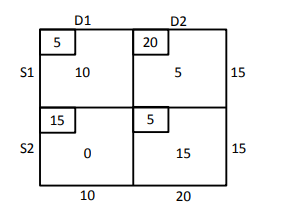
\includegraphics[width=0.75\columnwidth]{chapters/10/7/2/4/figs/fig.png}
 \end{center}
\caption{}
\label{fig:10/7/2/4Fig1}
\end{figure}
\fi

\item Find the position vector of the mid point of the vector joining the points $\vec{P}$(2, 3, 4)
and $\vec{Q}$(4, 1, –2).
\\
\solution
		\begin{enumerate}[label=\thesubsection.\arabic*,ref=\thesubsection.\theenumi]
\item Find the coordinates of the point which divides the join of $(-1,7) $ and $ (4,-3)$ in the ratio 2:3.
	\\
		\solution
	\input{chapters/10/7/2/1/section.tex}
\item Find the coordinates of the point $\vec{R}$ on the line segment joining the points $\vec{P}(-1,3)$ and $\vec{Q}(2,5)$ such that $PR=\frac{3}{5}PQ$.
\item Find the ratio in which the point $\vec{P}\brak{\frac{3}{4},\frac{5}{12}}$ divides the line segment joining the points $\vec{A}\brak{\frac{1}{2},\frac{3}{2}}$ and $ \vec{B}(2,-5)$.
\item Find the coordinates of the point which divides the line segment joining the points $(4,-3)$ and $(8,5)$ in the ratio $3:1$ internally.
\item Find the coordinates of the point $\vec{P}$ on $AD$ such that $AP : PD = 2 : 1$.
\item If the point $\vec{P} (2, 1)$ lies on the line segment joining points $\vec{A} (4, 2)$  and $ \vec{B} (8, 4)$,
then
\begin{enumerate}
	\item $AP =\frac{1}{3}{AB}$ 
\item ${AP}={PE}$
\item ${PB}=\frac{1}{3}{AB}$
\item${AP}=\frac{1}{2}{AB}$
 \end{enumerate}
\item Find the ratio in which the line segment joining the points $(-3,10)$  and  $(6,-8)$  is divided by $ (-1,6)$.
	\\
		\solution
	\input{chapters/10/7/2/4/section.tex}
\item Find the position vector of the mid point of the vector joining the points $\vec{P}$(2, 3, 4)
and $\vec{Q}$(4, 1, –2).
\\
\solution
		\input{chapters/12/10/2/16/section.tex}
\item Let $\vec{A}(4, 2), \vec{B}(6, 5)$  and $ \vec{C}(1, 4)$ be the vertices of $\triangle ABC$.
\begin{enumerate}
\item If $\vec{A}$ and  $\vec{B}$ are $(-2,-2)$ and  $(2,-4)$, respectively, find the coordinates of $\vec{P}$ such that $AP= \frac {3}{7}AB$  and $ \vec{P}$ lies on the line segment $AB$.
	\\
		\solution
	\input{chapters/10/7/2/8/section.tex}
\item Find the coordinates of the points which divide the line segment joining $A(-2,2)$  and  $\vec{B}(2,8)$ into four equal parts.
	\\
		\solution
	\input{chapters/10/7/2/9/section.tex}
\item In what ratio does the point $(-4,6)$ divide the line segment joining the points $\vec{A}(-6,0)$ and $\vec{B}(3,-8)$?
\item Given that $\vec{P}(3,2,-4), \vec{Q}(5,4,-6)$ and $\vec{R}(9,8,-10)$ are collinear. Find the ratio in which $\vec{Q}$ divides $PR$.
\item Points $\vec{A}(-6,10),\vec{B}(-4,6)$  and  $\vec{C}(3,-8)$ are collinear such that $AB=  \frac{2}{9}AC$.
\item The point which divides the line segment joining the points $\vec{P} (7, –6) $  and  $\vec{Q}(3, 4)$ in the 
ratio 1 : 2 internally lies in  which quadrant?
\item Find the coordinates of the points of trisection of the line segment joining $(4,-1)$  and  $(-2,3)$.
	\\
		\solution
	\input{chapters/10/7/2/2/section.tex}
\item Find the coordinates of the points which trisect the line segment joining the points $\vec{P}(4,2,-6)$ and $\vec{Q}(10,-16,6)$.
\item Find the coordinates of the points of trisection (i.e. points dividing to three equal parts) of the line segment joining the points $\vec{A}(2,-2)$ and $\vec{B}(-7,4)$.
\item Point $\vec{P}(5,-3)$ is one of the two points of trisection of line segment joining the points $\vec{A}(7,-2)$ and $\vec{B}(1,-5)$
\item Find the position vector of a point $\vec{R}$ which divides the line joining two points $\vec{P}$
and $\vec{Q}$ whose position vectors are $\hat{i}+2\hat{j}-\hat{k}$ and $-\hat{i}+\hat{j}+\hat{k}$ respectively, in the
ratio 2 : 1
\begin{enumerate}
    \item  internally
    \item  externally
\end{enumerate}
%\solution
%		\input{chapters/12/10/2/15/section.tex}
\item Find the coordinates of the point which divides the line segment joining the points which divides the line segment joining  the points $(-2,3,5)$ and $(1,-4,6)$ in the ratio 
\begin{enumerate}
\item $2:3$ internally,
\item $2:3$ externally
\end{enumerate}
\item Find the coordinates of the point which divides the line segment joining the points $(1,-2,3)$ and $(3,4,-5)$ in the ratio $2:3$
\begin{enumerate}
\item internally, and
\item externally
\end{enumerate}
\item Consider two points $\vec{P}$ and $\vec{Q}$ with position vectors $\overrightarrow{OP} = 3\overrightarrow{a}-2\overrightarrow{b}$ and $\overrightarrow{OQ}=\overrightarrow{a}+\overrightarrow{b}$. Find the position vector of a point $\vec{R}$ which divides the line joining $\vec{P}$ and $\vec{Q}$ in the ratio $2:1$, 
\begin{enumerate}
\item internally, and 
\item externally.
\end{enumerate}
\item The median from $\vec{A}$ meets $BC$ at $\vec{D}$. Find the coordinates of the point $\vec{D}$.
\item Find the coordinates of points $\vec{Q}$ and $\vec{R}$ on medians $BE$ and $CF$ respectively such that $BQ : QE = 2 : 1$  and  $CR : RF = 2 : 1$.
\item What do you observe?
\item If $\vec{A}, \vec{B}$ and $\vec{C}$  are the vertices of $\triangle ABC$, find the coordinates of the centroid of the triangle.
\end{enumerate}
\solution
	\input{chapters/10/7/4/7/section.tex}
\item If $\vec{P}(9a-2,-b)$ divides line segment joining $\vec{A}(3a+1,-3)$ and $\vec{B}(8a,5)$ in the ratio 3:1, find the values of $a$ and $b$.
\item Find the position vector of a point $\vec{R}$ which divides the line joining two points $\vec{P}$ and $\vec{Q}$ whose position vectors are $2\vec{a}+\vec{b}$ and $\vec{a}-3\vec{b}$ externally in the ratio $1:2$.
\item The position vector of the point which divides the join of points 2$\vec{a}$-3$\vec{b}$ $\text{and}$ $\vec{a}+\vec{b}$ in the ratio 3:1 is \rule{1cm}{0.1pt}.
\item If $\vec{a}$ and $\vec{b}$ are the postion vectors of $\vec{A}$ and $\vec{B}$, respectively, find the position vector of a point $\vec{C}$ in $BA$ produced such that $BC=1.5BA$.
\item Find the position vector of a point $\vec{R}$ which divides the line joining two points $\vec{P}$ and $\vec{Q}$ whose position vectors are $(2\vec{a}+\vec{b})$ and $(\vec{a}-3\vec{b})$
externally in the ratio 1 : 2. Also, show that $\vec{P}$ is the mid point of the line segment $RQ$.
\end{enumerate}

\item Let $\vec{A}(4, 2), \vec{B}(6, 5)$  and $ \vec{C}(1, 4)$ be the vertices of $\triangle ABC$.
\begin{enumerate}
\item If $\vec{A}$ and  $\vec{B}$ are $(-2,-2)$ and  $(2,-4)$, respectively, find the coordinates of $\vec{P}$ such that $AP= \frac {3}{7}AB$  and $ \vec{P}$ lies on the line segment $AB$.
	\\
		\solution
	\begin{enumerate}[label=\thesubsection.\arabic*,ref=\thesubsection.\theenumi]
\item Find the coordinates of the point which divides the join of $(-1,7) $ and $ (4,-3)$ in the ratio 2:3.
	\\
		\solution
	\input{chapters/10/7/2/1/section.tex}
\item Find the coordinates of the point $\vec{R}$ on the line segment joining the points $\vec{P}(-1,3)$ and $\vec{Q}(2,5)$ such that $PR=\frac{3}{5}PQ$.
\item Find the ratio in which the point $\vec{P}\brak{\frac{3}{4},\frac{5}{12}}$ divides the line segment joining the points $\vec{A}\brak{\frac{1}{2},\frac{3}{2}}$ and $ \vec{B}(2,-5)$.
\item Find the coordinates of the point which divides the line segment joining the points $(4,-3)$ and $(8,5)$ in the ratio $3:1$ internally.
\item Find the coordinates of the point $\vec{P}$ on $AD$ such that $AP : PD = 2 : 1$.
\item If the point $\vec{P} (2, 1)$ lies on the line segment joining points $\vec{A} (4, 2)$  and $ \vec{B} (8, 4)$,
then
\begin{enumerate}
	\item $AP =\frac{1}{3}{AB}$ 
\item ${AP}={PE}$
\item ${PB}=\frac{1}{3}{AB}$
\item${AP}=\frac{1}{2}{AB}$
 \end{enumerate}
\item Find the ratio in which the line segment joining the points $(-3,10)$  and  $(6,-8)$  is divided by $ (-1,6)$.
	\\
		\solution
	\input{chapters/10/7/2/4/section.tex}
\item Find the position vector of the mid point of the vector joining the points $\vec{P}$(2, 3, 4)
and $\vec{Q}$(4, 1, –2).
\\
\solution
		\input{chapters/12/10/2/16/section.tex}
\item Let $\vec{A}(4, 2), \vec{B}(6, 5)$  and $ \vec{C}(1, 4)$ be the vertices of $\triangle ABC$.
\begin{enumerate}
\item If $\vec{A}$ and  $\vec{B}$ are $(-2,-2)$ and  $(2,-4)$, respectively, find the coordinates of $\vec{P}$ such that $AP= \frac {3}{7}AB$  and $ \vec{P}$ lies on the line segment $AB$.
	\\
		\solution
	\input{chapters/10/7/2/8/section.tex}
\item Find the coordinates of the points which divide the line segment joining $A(-2,2)$  and  $\vec{B}(2,8)$ into four equal parts.
	\\
		\solution
	\input{chapters/10/7/2/9/section.tex}
\item In what ratio does the point $(-4,6)$ divide the line segment joining the points $\vec{A}(-6,0)$ and $\vec{B}(3,-8)$?
\item Given that $\vec{P}(3,2,-4), \vec{Q}(5,4,-6)$ and $\vec{R}(9,8,-10)$ are collinear. Find the ratio in which $\vec{Q}$ divides $PR$.
\item Points $\vec{A}(-6,10),\vec{B}(-4,6)$  and  $\vec{C}(3,-8)$ are collinear such that $AB=  \frac{2}{9}AC$.
\item The point which divides the line segment joining the points $\vec{P} (7, –6) $  and  $\vec{Q}(3, 4)$ in the 
ratio 1 : 2 internally lies in  which quadrant?
\item Find the coordinates of the points of trisection of the line segment joining $(4,-1)$  and  $(-2,3)$.
	\\
		\solution
	\input{chapters/10/7/2/2/section.tex}
\item Find the coordinates of the points which trisect the line segment joining the points $\vec{P}(4,2,-6)$ and $\vec{Q}(10,-16,6)$.
\item Find the coordinates of the points of trisection (i.e. points dividing to three equal parts) of the line segment joining the points $\vec{A}(2,-2)$ and $\vec{B}(-7,4)$.
\item Point $\vec{P}(5,-3)$ is one of the two points of trisection of line segment joining the points $\vec{A}(7,-2)$ and $\vec{B}(1,-5)$
\item Find the position vector of a point $\vec{R}$ which divides the line joining two points $\vec{P}$
and $\vec{Q}$ whose position vectors are $\hat{i}+2\hat{j}-\hat{k}$ and $-\hat{i}+\hat{j}+\hat{k}$ respectively, in the
ratio 2 : 1
\begin{enumerate}
    \item  internally
    \item  externally
\end{enumerate}
%\solution
%		\input{chapters/12/10/2/15/section.tex}
\item Find the coordinates of the point which divides the line segment joining the points which divides the line segment joining  the points $(-2,3,5)$ and $(1,-4,6)$ in the ratio 
\begin{enumerate}
\item $2:3$ internally,
\item $2:3$ externally
\end{enumerate}
\item Find the coordinates of the point which divides the line segment joining the points $(1,-2,3)$ and $(3,4,-5)$ in the ratio $2:3$
\begin{enumerate}
\item internally, and
\item externally
\end{enumerate}
\item Consider two points $\vec{P}$ and $\vec{Q}$ with position vectors $\overrightarrow{OP} = 3\overrightarrow{a}-2\overrightarrow{b}$ and $\overrightarrow{OQ}=\overrightarrow{a}+\overrightarrow{b}$. Find the position vector of a point $\vec{R}$ which divides the line joining $\vec{P}$ and $\vec{Q}$ in the ratio $2:1$, 
\begin{enumerate}
\item internally, and 
\item externally.
\end{enumerate}
\item The median from $\vec{A}$ meets $BC$ at $\vec{D}$. Find the coordinates of the point $\vec{D}$.
\item Find the coordinates of points $\vec{Q}$ and $\vec{R}$ on medians $BE$ and $CF$ respectively such that $BQ : QE = 2 : 1$  and  $CR : RF = 2 : 1$.
\item What do you observe?
\item If $\vec{A}, \vec{B}$ and $\vec{C}$  are the vertices of $\triangle ABC$, find the coordinates of the centroid of the triangle.
\end{enumerate}
\solution
	\input{chapters/10/7/4/7/section.tex}
\item If $\vec{P}(9a-2,-b)$ divides line segment joining $\vec{A}(3a+1,-3)$ and $\vec{B}(8a,5)$ in the ratio 3:1, find the values of $a$ and $b$.
\item Find the position vector of a point $\vec{R}$ which divides the line joining two points $\vec{P}$ and $\vec{Q}$ whose position vectors are $2\vec{a}+\vec{b}$ and $\vec{a}-3\vec{b}$ externally in the ratio $1:2$.
\item The position vector of the point which divides the join of points 2$\vec{a}$-3$\vec{b}$ $\text{and}$ $\vec{a}+\vec{b}$ in the ratio 3:1 is \rule{1cm}{0.1pt}.
\item If $\vec{a}$ and $\vec{b}$ are the postion vectors of $\vec{A}$ and $\vec{B}$, respectively, find the position vector of a point $\vec{C}$ in $BA$ produced such that $BC=1.5BA$.
\item Find the position vector of a point $\vec{R}$ which divides the line joining two points $\vec{P}$ and $\vec{Q}$ whose position vectors are $(2\vec{a}+\vec{b})$ and $(\vec{a}-3\vec{b})$
externally in the ratio 1 : 2. Also, show that $\vec{P}$ is the mid point of the line segment $RQ$.
\end{enumerate}

\item Find the coordinates of the points which divide the line segment joining $A(-2,2)$  and  $\vec{B}(2,8)$ into four equal parts.
	\\
		\solution
	\begin{enumerate}[label=\thesubsection.\arabic*,ref=\thesubsection.\theenumi]
\item Find the coordinates of the point which divides the join of $(-1,7) $ and $ (4,-3)$ in the ratio 2:3.
	\\
		\solution
	\input{chapters/10/7/2/1/section.tex}
\item Find the coordinates of the point $\vec{R}$ on the line segment joining the points $\vec{P}(-1,3)$ and $\vec{Q}(2,5)$ such that $PR=\frac{3}{5}PQ$.
\item Find the ratio in which the point $\vec{P}\brak{\frac{3}{4},\frac{5}{12}}$ divides the line segment joining the points $\vec{A}\brak{\frac{1}{2},\frac{3}{2}}$ and $ \vec{B}(2,-5)$.
\item Find the coordinates of the point which divides the line segment joining the points $(4,-3)$ and $(8,5)$ in the ratio $3:1$ internally.
\item Find the coordinates of the point $\vec{P}$ on $AD$ such that $AP : PD = 2 : 1$.
\item If the point $\vec{P} (2, 1)$ lies on the line segment joining points $\vec{A} (4, 2)$  and $ \vec{B} (8, 4)$,
then
\begin{enumerate}
	\item $AP =\frac{1}{3}{AB}$ 
\item ${AP}={PE}$
\item ${PB}=\frac{1}{3}{AB}$
\item${AP}=\frac{1}{2}{AB}$
 \end{enumerate}
\item Find the ratio in which the line segment joining the points $(-3,10)$  and  $(6,-8)$  is divided by $ (-1,6)$.
	\\
		\solution
	\input{chapters/10/7/2/4/section.tex}
\item Find the position vector of the mid point of the vector joining the points $\vec{P}$(2, 3, 4)
and $\vec{Q}$(4, 1, –2).
\\
\solution
		\input{chapters/12/10/2/16/section.tex}
\item Let $\vec{A}(4, 2), \vec{B}(6, 5)$  and $ \vec{C}(1, 4)$ be the vertices of $\triangle ABC$.
\begin{enumerate}
\item If $\vec{A}$ and  $\vec{B}$ are $(-2,-2)$ and  $(2,-4)$, respectively, find the coordinates of $\vec{P}$ such that $AP= \frac {3}{7}AB$  and $ \vec{P}$ lies on the line segment $AB$.
	\\
		\solution
	\input{chapters/10/7/2/8/section.tex}
\item Find the coordinates of the points which divide the line segment joining $A(-2,2)$  and  $\vec{B}(2,8)$ into four equal parts.
	\\
		\solution
	\input{chapters/10/7/2/9/section.tex}
\item In what ratio does the point $(-4,6)$ divide the line segment joining the points $\vec{A}(-6,0)$ and $\vec{B}(3,-8)$?
\item Given that $\vec{P}(3,2,-4), \vec{Q}(5,4,-6)$ and $\vec{R}(9,8,-10)$ are collinear. Find the ratio in which $\vec{Q}$ divides $PR$.
\item Points $\vec{A}(-6,10),\vec{B}(-4,6)$  and  $\vec{C}(3,-8)$ are collinear such that $AB=  \frac{2}{9}AC$.
\item The point which divides the line segment joining the points $\vec{P} (7, –6) $  and  $\vec{Q}(3, 4)$ in the 
ratio 1 : 2 internally lies in  which quadrant?
\item Find the coordinates of the points of trisection of the line segment joining $(4,-1)$  and  $(-2,3)$.
	\\
		\solution
	\input{chapters/10/7/2/2/section.tex}
\item Find the coordinates of the points which trisect the line segment joining the points $\vec{P}(4,2,-6)$ and $\vec{Q}(10,-16,6)$.
\item Find the coordinates of the points of trisection (i.e. points dividing to three equal parts) of the line segment joining the points $\vec{A}(2,-2)$ and $\vec{B}(-7,4)$.
\item Point $\vec{P}(5,-3)$ is one of the two points of trisection of line segment joining the points $\vec{A}(7,-2)$ and $\vec{B}(1,-5)$
\item Find the position vector of a point $\vec{R}$ which divides the line joining two points $\vec{P}$
and $\vec{Q}$ whose position vectors are $\hat{i}+2\hat{j}-\hat{k}$ and $-\hat{i}+\hat{j}+\hat{k}$ respectively, in the
ratio 2 : 1
\begin{enumerate}
    \item  internally
    \item  externally
\end{enumerate}
%\solution
%		\input{chapters/12/10/2/15/section.tex}
\item Find the coordinates of the point which divides the line segment joining the points which divides the line segment joining  the points $(-2,3,5)$ and $(1,-4,6)$ in the ratio 
\begin{enumerate}
\item $2:3$ internally,
\item $2:3$ externally
\end{enumerate}
\item Find the coordinates of the point which divides the line segment joining the points $(1,-2,3)$ and $(3,4,-5)$ in the ratio $2:3$
\begin{enumerate}
\item internally, and
\item externally
\end{enumerate}
\item Consider two points $\vec{P}$ and $\vec{Q}$ with position vectors $\overrightarrow{OP} = 3\overrightarrow{a}-2\overrightarrow{b}$ and $\overrightarrow{OQ}=\overrightarrow{a}+\overrightarrow{b}$. Find the position vector of a point $\vec{R}$ which divides the line joining $\vec{P}$ and $\vec{Q}$ in the ratio $2:1$, 
\begin{enumerate}
\item internally, and 
\item externally.
\end{enumerate}
\item The median from $\vec{A}$ meets $BC$ at $\vec{D}$. Find the coordinates of the point $\vec{D}$.
\item Find the coordinates of points $\vec{Q}$ and $\vec{R}$ on medians $BE$ and $CF$ respectively such that $BQ : QE = 2 : 1$  and  $CR : RF = 2 : 1$.
\item What do you observe?
\item If $\vec{A}, \vec{B}$ and $\vec{C}$  are the vertices of $\triangle ABC$, find the coordinates of the centroid of the triangle.
\end{enumerate}
\solution
	\input{chapters/10/7/4/7/section.tex}
\item If $\vec{P}(9a-2,-b)$ divides line segment joining $\vec{A}(3a+1,-3)$ and $\vec{B}(8a,5)$ in the ratio 3:1, find the values of $a$ and $b$.
\item Find the position vector of a point $\vec{R}$ which divides the line joining two points $\vec{P}$ and $\vec{Q}$ whose position vectors are $2\vec{a}+\vec{b}$ and $\vec{a}-3\vec{b}$ externally in the ratio $1:2$.
\item The position vector of the point which divides the join of points 2$\vec{a}$-3$\vec{b}$ $\text{and}$ $\vec{a}+\vec{b}$ in the ratio 3:1 is \rule{1cm}{0.1pt}.
\item If $\vec{a}$ and $\vec{b}$ are the postion vectors of $\vec{A}$ and $\vec{B}$, respectively, find the position vector of a point $\vec{C}$ in $BA$ produced such that $BC=1.5BA$.
\item Find the position vector of a point $\vec{R}$ which divides the line joining two points $\vec{P}$ and $\vec{Q}$ whose position vectors are $(2\vec{a}+\vec{b})$ and $(\vec{a}-3\vec{b})$
externally in the ratio 1 : 2. Also, show that $\vec{P}$ is the mid point of the line segment $RQ$.
\end{enumerate}

\item In what ratio does the point $(-4,6)$ divide the line segment joining the points $\vec{A}(-6,0)$ and $\vec{B}(3,-8)$?
\item Given that $\vec{P}(3,2,-4), \vec{Q}(5,4,-6)$ and $\vec{R}(9,8,-10)$ are collinear. Find the ratio in which $\vec{Q}$ divides $PR$.
\item Points $\vec{A}(-6,10),\vec{B}(-4,6)$  and  $\vec{C}(3,-8)$ are collinear such that $AB=  \frac{2}{9}AC$.
\item The point which divides the line segment joining the points $\vec{P} (7, –6) $  and  $\vec{Q}(3, 4)$ in the 
ratio 1 : 2 internally lies in  which quadrant?
\item Find the coordinates of the points of trisection of the line segment joining $(4,-1)$  and  $(-2,3)$.
	\\
		\solution
	Using section formula,
\begin{align}
\vec{R}=\frac{1}{1+\frac{1}{2}}\brak{\myvec{4\\-1}+\frac{1}{2}\myvec{-2\\3}}
=\myvec{2\\ \frac{1}{3}}\\
\vec{S}=\frac{1}{1+\frac{2}{1}}\brak{\myvec{4\\-1}+\frac{2}{1}\myvec{-2\\3}}
=\myvec{0\\ \frac{5}{3}}
\end{align}
which are the desired points of trisection.
\iffalse
See
		\figref{fig:chapters/10/7/2/2/Figure}
\begin{figure}[H]
\centering
\includegraphics[width=0.75\columnwidth]{chapters/10/7/2/2/figs/dj.pdf}
\caption{}
		\label{fig:chapters/10/7/2/2/Figure}
\end{figure}
\fi

\item Find the coordinates of the points which trisect the line segment joining the points $\vec{P}(4,2,-6)$ and $\vec{Q}(10,-16,6)$.
\item Find the coordinates of the points of trisection (i.e. points dividing to three equal parts) of the line segment joining the points $\vec{A}(2,-2)$ and $\vec{B}(-7,4)$.
\item Point $\vec{P}(5,-3)$ is one of the two points of trisection of line segment joining the points $\vec{A}(7,-2)$ and $\vec{B}(1,-5)$
\item Find the position vector of a point $\vec{R}$ which divides the line joining two points $\vec{P}$
and $\vec{Q}$ whose position vectors are $\hat{i}+2\hat{j}-\hat{k}$ and $-\hat{i}+\hat{j}+\hat{k}$ respectively, in the
ratio 2 : 1
\begin{enumerate}
    \item  internally
    \item  externally
\end{enumerate}
%\solution
%		\begin{enumerate}[label=\thesubsection.\arabic*,ref=\thesubsection.\theenumi]
\item Find the coordinates of the point which divides the join of $(-1,7) $ and $ (4,-3)$ in the ratio 2:3.
	\\
		\solution
	\input{chapters/10/7/2/1/section.tex}
\item Find the coordinates of the point $\vec{R}$ on the line segment joining the points $\vec{P}(-1,3)$ and $\vec{Q}(2,5)$ such that $PR=\frac{3}{5}PQ$.
\item Find the ratio in which the point $\vec{P}\brak{\frac{3}{4},\frac{5}{12}}$ divides the line segment joining the points $\vec{A}\brak{\frac{1}{2},\frac{3}{2}}$ and $ \vec{B}(2,-5)$.
\item Find the coordinates of the point which divides the line segment joining the points $(4,-3)$ and $(8,5)$ in the ratio $3:1$ internally.
\item Find the coordinates of the point $\vec{P}$ on $AD$ such that $AP : PD = 2 : 1$.
\item If the point $\vec{P} (2, 1)$ lies on the line segment joining points $\vec{A} (4, 2)$  and $ \vec{B} (8, 4)$,
then
\begin{enumerate}
	\item $AP =\frac{1}{3}{AB}$ 
\item ${AP}={PE}$
\item ${PB}=\frac{1}{3}{AB}$
\item${AP}=\frac{1}{2}{AB}$
 \end{enumerate}
\item Find the ratio in which the line segment joining the points $(-3,10)$  and  $(6,-8)$  is divided by $ (-1,6)$.
	\\
		\solution
	\input{chapters/10/7/2/4/section.tex}
\item Find the position vector of the mid point of the vector joining the points $\vec{P}$(2, 3, 4)
and $\vec{Q}$(4, 1, –2).
\\
\solution
		\input{chapters/12/10/2/16/section.tex}
\item Let $\vec{A}(4, 2), \vec{B}(6, 5)$  and $ \vec{C}(1, 4)$ be the vertices of $\triangle ABC$.
\begin{enumerate}
\item If $\vec{A}$ and  $\vec{B}$ are $(-2,-2)$ and  $(2,-4)$, respectively, find the coordinates of $\vec{P}$ such that $AP= \frac {3}{7}AB$  and $ \vec{P}$ lies on the line segment $AB$.
	\\
		\solution
	\input{chapters/10/7/2/8/section.tex}
\item Find the coordinates of the points which divide the line segment joining $A(-2,2)$  and  $\vec{B}(2,8)$ into four equal parts.
	\\
		\solution
	\input{chapters/10/7/2/9/section.tex}
\item In what ratio does the point $(-4,6)$ divide the line segment joining the points $\vec{A}(-6,0)$ and $\vec{B}(3,-8)$?
\item Given that $\vec{P}(3,2,-4), \vec{Q}(5,4,-6)$ and $\vec{R}(9,8,-10)$ are collinear. Find the ratio in which $\vec{Q}$ divides $PR$.
\item Points $\vec{A}(-6,10),\vec{B}(-4,6)$  and  $\vec{C}(3,-8)$ are collinear such that $AB=  \frac{2}{9}AC$.
\item The point which divides the line segment joining the points $\vec{P} (7, –6) $  and  $\vec{Q}(3, 4)$ in the 
ratio 1 : 2 internally lies in  which quadrant?
\item Find the coordinates of the points of trisection of the line segment joining $(4,-1)$  and  $(-2,3)$.
	\\
		\solution
	\input{chapters/10/7/2/2/section.tex}
\item Find the coordinates of the points which trisect the line segment joining the points $\vec{P}(4,2,-6)$ and $\vec{Q}(10,-16,6)$.
\item Find the coordinates of the points of trisection (i.e. points dividing to three equal parts) of the line segment joining the points $\vec{A}(2,-2)$ and $\vec{B}(-7,4)$.
\item Point $\vec{P}(5,-3)$ is one of the two points of trisection of line segment joining the points $\vec{A}(7,-2)$ and $\vec{B}(1,-5)$
\item Find the position vector of a point $\vec{R}$ which divides the line joining two points $\vec{P}$
and $\vec{Q}$ whose position vectors are $\hat{i}+2\hat{j}-\hat{k}$ and $-\hat{i}+\hat{j}+\hat{k}$ respectively, in the
ratio 2 : 1
\begin{enumerate}
    \item  internally
    \item  externally
\end{enumerate}
%\solution
%		\input{chapters/12/10/2/15/section.tex}
\item Find the coordinates of the point which divides the line segment joining the points which divides the line segment joining  the points $(-2,3,5)$ and $(1,-4,6)$ in the ratio 
\begin{enumerate}
\item $2:3$ internally,
\item $2:3$ externally
\end{enumerate}
\item Find the coordinates of the point which divides the line segment joining the points $(1,-2,3)$ and $(3,4,-5)$ in the ratio $2:3$
\begin{enumerate}
\item internally, and
\item externally
\end{enumerate}
\item Consider two points $\vec{P}$ and $\vec{Q}$ with position vectors $\overrightarrow{OP} = 3\overrightarrow{a}-2\overrightarrow{b}$ and $\overrightarrow{OQ}=\overrightarrow{a}+\overrightarrow{b}$. Find the position vector of a point $\vec{R}$ which divides the line joining $\vec{P}$ and $\vec{Q}$ in the ratio $2:1$, 
\begin{enumerate}
\item internally, and 
\item externally.
\end{enumerate}
\item The median from $\vec{A}$ meets $BC$ at $\vec{D}$. Find the coordinates of the point $\vec{D}$.
\item Find the coordinates of points $\vec{Q}$ and $\vec{R}$ on medians $BE$ and $CF$ respectively such that $BQ : QE = 2 : 1$  and  $CR : RF = 2 : 1$.
\item What do you observe?
\item If $\vec{A}, \vec{B}$ and $\vec{C}$  are the vertices of $\triangle ABC$, find the coordinates of the centroid of the triangle.
\end{enumerate}
\solution
	\input{chapters/10/7/4/7/section.tex}
\item If $\vec{P}(9a-2,-b)$ divides line segment joining $\vec{A}(3a+1,-3)$ and $\vec{B}(8a,5)$ in the ratio 3:1, find the values of $a$ and $b$.
\item Find the position vector of a point $\vec{R}$ which divides the line joining two points $\vec{P}$ and $\vec{Q}$ whose position vectors are $2\vec{a}+\vec{b}$ and $\vec{a}-3\vec{b}$ externally in the ratio $1:2$.
\item The position vector of the point which divides the join of points 2$\vec{a}$-3$\vec{b}$ $\text{and}$ $\vec{a}+\vec{b}$ in the ratio 3:1 is \rule{1cm}{0.1pt}.
\item If $\vec{a}$ and $\vec{b}$ are the postion vectors of $\vec{A}$ and $\vec{B}$, respectively, find the position vector of a point $\vec{C}$ in $BA$ produced such that $BC=1.5BA$.
\item Find the position vector of a point $\vec{R}$ which divides the line joining two points $\vec{P}$ and $\vec{Q}$ whose position vectors are $(2\vec{a}+\vec{b})$ and $(\vec{a}-3\vec{b})$
externally in the ratio 1 : 2. Also, show that $\vec{P}$ is the mid point of the line segment $RQ$.
\end{enumerate}

\item Find the coordinates of the point which divides the line segment joining the points which divides the line segment joining  the points $(-2,3,5)$ and $(1,-4,6)$ in the ratio 
\begin{enumerate}
\item $2:3$ internally,
\item $2:3$ externally
\end{enumerate}
\item Find the coordinates of the point which divides the line segment joining the points $(1,-2,3)$ and $(3,4,-5)$ in the ratio $2:3$
\begin{enumerate}
\item internally, and
\item externally
\end{enumerate}
\item Consider two points $\vec{P}$ and $\vec{Q}$ with position vectors $\overrightarrow{OP} = 3\overrightarrow{a}-2\overrightarrow{b}$ and $\overrightarrow{OQ}=\overrightarrow{a}+\overrightarrow{b}$. Find the position vector of a point $\vec{R}$ which divides the line joining $\vec{P}$ and $\vec{Q}$ in the ratio $2:1$, 
\begin{enumerate}
\item internally, and 
\item externally.
\end{enumerate}
\item The median from $\vec{A}$ meets $BC$ at $\vec{D}$. Find the coordinates of the point $\vec{D}$.
\item Find the coordinates of points $\vec{Q}$ and $\vec{R}$ on medians $BE$ and $CF$ respectively such that $BQ : QE = 2 : 1$  and  $CR : RF = 2 : 1$.
\item What do you observe?
\item If $\vec{A}, \vec{B}$ and $\vec{C}$  are the vertices of $\triangle ABC$, find the coordinates of the centroid of the triangle.
\end{enumerate}
\solution
	\begin{enumerate}[label=\thesubsection.\arabic*,ref=\thesubsection.\theenumi]
\item Find the coordinates of the point which divides the join of $(-1,7) $ and $ (4,-3)$ in the ratio 2:3.
	\\
		\solution
	\input{chapters/10/7/2/1/section.tex}
\item Find the coordinates of the point $\vec{R}$ on the line segment joining the points $\vec{P}(-1,3)$ and $\vec{Q}(2,5)$ such that $PR=\frac{3}{5}PQ$.
\item Find the ratio in which the point $\vec{P}\brak{\frac{3}{4},\frac{5}{12}}$ divides the line segment joining the points $\vec{A}\brak{\frac{1}{2},\frac{3}{2}}$ and $ \vec{B}(2,-5)$.
\item Find the coordinates of the point which divides the line segment joining the points $(4,-3)$ and $(8,5)$ in the ratio $3:1$ internally.
\item Find the coordinates of the point $\vec{P}$ on $AD$ such that $AP : PD = 2 : 1$.
\item If the point $\vec{P} (2, 1)$ lies on the line segment joining points $\vec{A} (4, 2)$  and $ \vec{B} (8, 4)$,
then
\begin{enumerate}
	\item $AP =\frac{1}{3}{AB}$ 
\item ${AP}={PE}$
\item ${PB}=\frac{1}{3}{AB}$
\item${AP}=\frac{1}{2}{AB}$
 \end{enumerate}
\item Find the ratio in which the line segment joining the points $(-3,10)$  and  $(6,-8)$  is divided by $ (-1,6)$.
	\\
		\solution
	\input{chapters/10/7/2/4/section.tex}
\item Find the position vector of the mid point of the vector joining the points $\vec{P}$(2, 3, 4)
and $\vec{Q}$(4, 1, –2).
\\
\solution
		\input{chapters/12/10/2/16/section.tex}
\item Let $\vec{A}(4, 2), \vec{B}(6, 5)$  and $ \vec{C}(1, 4)$ be the vertices of $\triangle ABC$.
\begin{enumerate}
\item If $\vec{A}$ and  $\vec{B}$ are $(-2,-2)$ and  $(2,-4)$, respectively, find the coordinates of $\vec{P}$ such that $AP= \frac {3}{7}AB$  and $ \vec{P}$ lies on the line segment $AB$.
	\\
		\solution
	\input{chapters/10/7/2/8/section.tex}
\item Find the coordinates of the points which divide the line segment joining $A(-2,2)$  and  $\vec{B}(2,8)$ into four equal parts.
	\\
		\solution
	\input{chapters/10/7/2/9/section.tex}
\item In what ratio does the point $(-4,6)$ divide the line segment joining the points $\vec{A}(-6,0)$ and $\vec{B}(3,-8)$?
\item Given that $\vec{P}(3,2,-4), \vec{Q}(5,4,-6)$ and $\vec{R}(9,8,-10)$ are collinear. Find the ratio in which $\vec{Q}$ divides $PR$.
\item Points $\vec{A}(-6,10),\vec{B}(-4,6)$  and  $\vec{C}(3,-8)$ are collinear such that $AB=  \frac{2}{9}AC$.
\item The point which divides the line segment joining the points $\vec{P} (7, –6) $  and  $\vec{Q}(3, 4)$ in the 
ratio 1 : 2 internally lies in  which quadrant?
\item Find the coordinates of the points of trisection of the line segment joining $(4,-1)$  and  $(-2,3)$.
	\\
		\solution
	\input{chapters/10/7/2/2/section.tex}
\item Find the coordinates of the points which trisect the line segment joining the points $\vec{P}(4,2,-6)$ and $\vec{Q}(10,-16,6)$.
\item Find the coordinates of the points of trisection (i.e. points dividing to three equal parts) of the line segment joining the points $\vec{A}(2,-2)$ and $\vec{B}(-7,4)$.
\item Point $\vec{P}(5,-3)$ is one of the two points of trisection of line segment joining the points $\vec{A}(7,-2)$ and $\vec{B}(1,-5)$
\item Find the position vector of a point $\vec{R}$ which divides the line joining two points $\vec{P}$
and $\vec{Q}$ whose position vectors are $\hat{i}+2\hat{j}-\hat{k}$ and $-\hat{i}+\hat{j}+\hat{k}$ respectively, in the
ratio 2 : 1
\begin{enumerate}
    \item  internally
    \item  externally
\end{enumerate}
%\solution
%		\input{chapters/12/10/2/15/section.tex}
\item Find the coordinates of the point which divides the line segment joining the points which divides the line segment joining  the points $(-2,3,5)$ and $(1,-4,6)$ in the ratio 
\begin{enumerate}
\item $2:3$ internally,
\item $2:3$ externally
\end{enumerate}
\item Find the coordinates of the point which divides the line segment joining the points $(1,-2,3)$ and $(3,4,-5)$ in the ratio $2:3$
\begin{enumerate}
\item internally, and
\item externally
\end{enumerate}
\item Consider two points $\vec{P}$ and $\vec{Q}$ with position vectors $\overrightarrow{OP} = 3\overrightarrow{a}-2\overrightarrow{b}$ and $\overrightarrow{OQ}=\overrightarrow{a}+\overrightarrow{b}$. Find the position vector of a point $\vec{R}$ which divides the line joining $\vec{P}$ and $\vec{Q}$ in the ratio $2:1$, 
\begin{enumerate}
\item internally, and 
\item externally.
\end{enumerate}
\item The median from $\vec{A}$ meets $BC$ at $\vec{D}$. Find the coordinates of the point $\vec{D}$.
\item Find the coordinates of points $\vec{Q}$ and $\vec{R}$ on medians $BE$ and $CF$ respectively such that $BQ : QE = 2 : 1$  and  $CR : RF = 2 : 1$.
\item What do you observe?
\item If $\vec{A}, \vec{B}$ and $\vec{C}$  are the vertices of $\triangle ABC$, find the coordinates of the centroid of the triangle.
\end{enumerate}
\solution
	\input{chapters/10/7/4/7/section.tex}
\item If $\vec{P}(9a-2,-b)$ divides line segment joining $\vec{A}(3a+1,-3)$ and $\vec{B}(8a,5)$ in the ratio 3:1, find the values of $a$ and $b$.
\item Find the position vector of a point $\vec{R}$ which divides the line joining two points $\vec{P}$ and $\vec{Q}$ whose position vectors are $2\vec{a}+\vec{b}$ and $\vec{a}-3\vec{b}$ externally in the ratio $1:2$.
\item The position vector of the point which divides the join of points 2$\vec{a}$-3$\vec{b}$ $\text{and}$ $\vec{a}+\vec{b}$ in the ratio 3:1 is \rule{1cm}{0.1pt}.
\item If $\vec{a}$ and $\vec{b}$ are the postion vectors of $\vec{A}$ and $\vec{B}$, respectively, find the position vector of a point $\vec{C}$ in $BA$ produced such that $BC=1.5BA$.
\item Find the position vector of a point $\vec{R}$ which divides the line joining two points $\vec{P}$ and $\vec{Q}$ whose position vectors are $(2\vec{a}+\vec{b})$ and $(\vec{a}-3\vec{b})$
externally in the ratio 1 : 2. Also, show that $\vec{P}$ is the mid point of the line segment $RQ$.
\end{enumerate}

\item If $\vec{P}(9a-2,-b)$ divides line segment joining $\vec{A}(3a+1,-3)$ and $\vec{B}(8a,5)$ in the ratio 3:1, find the values of $a$ and $b$.
\item Find the position vector of a point $\vec{R}$ which divides the line joining two points $\vec{P}$ and $\vec{Q}$ whose position vectors are $2\vec{a}+\vec{b}$ and $\vec{a}-3\vec{b}$ externally in the ratio $1:2$.
\item The position vector of the point which divides the join of points 2$\vec{a}$-3$\vec{b}$ $\text{and}$ $\vec{a}+\vec{b}$ in the ratio 3:1 is \rule{1cm}{0.1pt}.
\item If $\vec{a}$ and $\vec{b}$ are the postion vectors of $\vec{A}$ and $\vec{B}$, respectively, find the position vector of a point $\vec{C}$ in $BA$ produced such that $BC=1.5BA$.
\item Find the position vector of a point $\vec{R}$ which divides the line joining two points $\vec{P}$ and $\vec{Q}$ whose position vectors are $(2\vec{a}+\vec{b})$ and $(\vec{a}-3\vec{b})$
externally in the ratio 1 : 2. Also, show that $\vec{P}$ is the mid point of the line segment $RQ$.
\end{enumerate}

\item Find the coordinates of the point which divides the line segment joining the points which divides the line segment joining  the points $(-2,3,5)$ and $(1,-4,6)$ in the ratio 
\begin{enumerate}
\item $2:3$ internally,
\item $2:3$ externally
\end{enumerate}
\item Find the coordinates of the point which divides the line segment joining the points $(1,-2,3)$ and $(3,4,-5)$ in the ratio $2:3$
\begin{enumerate}
\item internally, and
\item externally
\end{enumerate}
\item Consider two points $\vec{P}$ and $\vec{Q}$ with position vectors $\overrightarrow{OP} = 3\overrightarrow{a}-2\overrightarrow{b}$ and $\overrightarrow{OQ}=\overrightarrow{a}+\overrightarrow{b}$. Find the position vector of a point $\vec{R}$ which divides the line joining $\vec{P}$ and $\vec{Q}$ in the ratio $2:1$, 
\begin{enumerate}
\item internally, and 
\item externally.
\end{enumerate}
\item The median from $\vec{A}$ meets $BC$ at $\vec{D}$. Find the coordinates of the point $\vec{D}$.
\item Find the coordinates of points $\vec{Q}$ and $\vec{R}$ on medians $BE$ and $CF$ respectively such that $BQ : QE = 2 : 1$  and  $CR : RF = 2 : 1$.
\item What do you observe?
\item If $\vec{A}, \vec{B}$ and $\vec{C}$  are the vertices of $\triangle ABC$, find the coordinates of the centroid of the triangle.
\end{enumerate}
\solution
	\begin{enumerate}[label=\thesubsection.\arabic*,ref=\thesubsection.\theenumi]
\item Find the coordinates of the point which divides the join of $(-1,7) $ and $ (4,-3)$ in the ratio 2:3.
	\\
		\solution
	\begin{enumerate}[label=\thesubsection.\arabic*,ref=\thesubsection.\theenumi]
\item Find the coordinates of the point which divides the join of $(-1,7) $ and $ (4,-3)$ in the ratio 2:3.
	\\
		\solution
	\input{chapters/10/7/2/1/section.tex}
\item Find the coordinates of the point $\vec{R}$ on the line segment joining the points $\vec{P}(-1,3)$ and $\vec{Q}(2,5)$ such that $PR=\frac{3}{5}PQ$.
\item Find the ratio in which the point $\vec{P}\brak{\frac{3}{4},\frac{5}{12}}$ divides the line segment joining the points $\vec{A}\brak{\frac{1}{2},\frac{3}{2}}$ and $ \vec{B}(2,-5)$.
\item Find the coordinates of the point which divides the line segment joining the points $(4,-3)$ and $(8,5)$ in the ratio $3:1$ internally.
\item Find the coordinates of the point $\vec{P}$ on $AD$ such that $AP : PD = 2 : 1$.
\item If the point $\vec{P} (2, 1)$ lies on the line segment joining points $\vec{A} (4, 2)$  and $ \vec{B} (8, 4)$,
then
\begin{enumerate}
	\item $AP =\frac{1}{3}{AB}$ 
\item ${AP}={PE}$
\item ${PB}=\frac{1}{3}{AB}$
\item${AP}=\frac{1}{2}{AB}$
 \end{enumerate}
\item Find the ratio in which the line segment joining the points $(-3,10)$  and  $(6,-8)$  is divided by $ (-1,6)$.
	\\
		\solution
	\input{chapters/10/7/2/4/section.tex}
\item Find the position vector of the mid point of the vector joining the points $\vec{P}$(2, 3, 4)
and $\vec{Q}$(4, 1, –2).
\\
\solution
		\input{chapters/12/10/2/16/section.tex}
\item Let $\vec{A}(4, 2), \vec{B}(6, 5)$  and $ \vec{C}(1, 4)$ be the vertices of $\triangle ABC$.
\begin{enumerate}
\item If $\vec{A}$ and  $\vec{B}$ are $(-2,-2)$ and  $(2,-4)$, respectively, find the coordinates of $\vec{P}$ such that $AP= \frac {3}{7}AB$  and $ \vec{P}$ lies on the line segment $AB$.
	\\
		\solution
	\input{chapters/10/7/2/8/section.tex}
\item Find the coordinates of the points which divide the line segment joining $A(-2,2)$  and  $\vec{B}(2,8)$ into four equal parts.
	\\
		\solution
	\input{chapters/10/7/2/9/section.tex}
\item In what ratio does the point $(-4,6)$ divide the line segment joining the points $\vec{A}(-6,0)$ and $\vec{B}(3,-8)$?
\item Given that $\vec{P}(3,2,-4), \vec{Q}(5,4,-6)$ and $\vec{R}(9,8,-10)$ are collinear. Find the ratio in which $\vec{Q}$ divides $PR$.
\item Points $\vec{A}(-6,10),\vec{B}(-4,6)$  and  $\vec{C}(3,-8)$ are collinear such that $AB=  \frac{2}{9}AC$.
\item The point which divides the line segment joining the points $\vec{P} (7, –6) $  and  $\vec{Q}(3, 4)$ in the 
ratio 1 : 2 internally lies in  which quadrant?
\item Find the coordinates of the points of trisection of the line segment joining $(4,-1)$  and  $(-2,3)$.
	\\
		\solution
	\input{chapters/10/7/2/2/section.tex}
\item Find the coordinates of the points which trisect the line segment joining the points $\vec{P}(4,2,-6)$ and $\vec{Q}(10,-16,6)$.
\item Find the coordinates of the points of trisection (i.e. points dividing to three equal parts) of the line segment joining the points $\vec{A}(2,-2)$ and $\vec{B}(-7,4)$.
\item Point $\vec{P}(5,-3)$ is one of the two points of trisection of line segment joining the points $\vec{A}(7,-2)$ and $\vec{B}(1,-5)$
\item Find the position vector of a point $\vec{R}$ which divides the line joining two points $\vec{P}$
and $\vec{Q}$ whose position vectors are $\hat{i}+2\hat{j}-\hat{k}$ and $-\hat{i}+\hat{j}+\hat{k}$ respectively, in the
ratio 2 : 1
\begin{enumerate}
    \item  internally
    \item  externally
\end{enumerate}
%\solution
%		\input{chapters/12/10/2/15/section.tex}
\item Find the coordinates of the point which divides the line segment joining the points which divides the line segment joining  the points $(-2,3,5)$ and $(1,-4,6)$ in the ratio 
\begin{enumerate}
\item $2:3$ internally,
\item $2:3$ externally
\end{enumerate}
\item Find the coordinates of the point which divides the line segment joining the points $(1,-2,3)$ and $(3,4,-5)$ in the ratio $2:3$
\begin{enumerate}
\item internally, and
\item externally
\end{enumerate}
\item Consider two points $\vec{P}$ and $\vec{Q}$ with position vectors $\overrightarrow{OP} = 3\overrightarrow{a}-2\overrightarrow{b}$ and $\overrightarrow{OQ}=\overrightarrow{a}+\overrightarrow{b}$. Find the position vector of a point $\vec{R}$ which divides the line joining $\vec{P}$ and $\vec{Q}$ in the ratio $2:1$, 
\begin{enumerate}
\item internally, and 
\item externally.
\end{enumerate}
\item The median from $\vec{A}$ meets $BC$ at $\vec{D}$. Find the coordinates of the point $\vec{D}$.
\item Find the coordinates of points $\vec{Q}$ and $\vec{R}$ on medians $BE$ and $CF$ respectively such that $BQ : QE = 2 : 1$  and  $CR : RF = 2 : 1$.
\item What do you observe?
\item If $\vec{A}, \vec{B}$ and $\vec{C}$  are the vertices of $\triangle ABC$, find the coordinates of the centroid of the triangle.
\end{enumerate}
\solution
	\input{chapters/10/7/4/7/section.tex}
\item If $\vec{P}(9a-2,-b)$ divides line segment joining $\vec{A}(3a+1,-3)$ and $\vec{B}(8a,5)$ in the ratio 3:1, find the values of $a$ and $b$.
\item Find the position vector of a point $\vec{R}$ which divides the line joining two points $\vec{P}$ and $\vec{Q}$ whose position vectors are $2\vec{a}+\vec{b}$ and $\vec{a}-3\vec{b}$ externally in the ratio $1:2$.
\item The position vector of the point which divides the join of points 2$\vec{a}$-3$\vec{b}$ $\text{and}$ $\vec{a}+\vec{b}$ in the ratio 3:1 is \rule{1cm}{0.1pt}.
\item If $\vec{a}$ and $\vec{b}$ are the postion vectors of $\vec{A}$ and $\vec{B}$, respectively, find the position vector of a point $\vec{C}$ in $BA$ produced such that $BC=1.5BA$.
\item Find the position vector of a point $\vec{R}$ which divides the line joining two points $\vec{P}$ and $\vec{Q}$ whose position vectors are $(2\vec{a}+\vec{b})$ and $(\vec{a}-3\vec{b})$
externally in the ratio 1 : 2. Also, show that $\vec{P}$ is the mid point of the line segment $RQ$.
\end{enumerate}

\item Find the coordinates of the point $\vec{R}$ on the line segment joining the points $\vec{P}(-1,3)$ and $\vec{Q}(2,5)$ such that $PR=\frac{3}{5}PQ$.
\item Find the ratio in which the point $\vec{P}\brak{\frac{3}{4},\frac{5}{12}}$ divides the line segment joining the points $\vec{A}\brak{\frac{1}{2},\frac{3}{2}}$ and $ \vec{B}(2,-5)$.
\item Find the coordinates of the point which divides the line segment joining the points $(4,-3)$ and $(8,5)$ in the ratio $3:1$ internally.
\item Find the coordinates of the point $\vec{P}$ on $AD$ such that $AP : PD = 2 : 1$.
\item If the point $\vec{P} (2, 1)$ lies on the line segment joining points $\vec{A} (4, 2)$  and $ \vec{B} (8, 4)$,
then
\begin{enumerate}
	\item $AP =\frac{1}{3}{AB}$ 
\item ${AP}={PE}$
\item ${PB}=\frac{1}{3}{AB}$
\item${AP}=\frac{1}{2}{AB}$
 \end{enumerate}
\item Find the ratio in which the line segment joining the points $(-3,10)$  and  $(6,-8)$  is divided by $ (-1,6)$.
	\\
		\solution
	\iffalse
Using section formula,
\begin{align}
         \myvec{-1\\6} &=\frac{{\myvec{-3\\10}+k\myvec{6\\-8}}}{1+k}\\
	 \implies 7k\myvec{1 \\ -2} &= 2\myvec{1 \\ -2}
	 \\
	 \text{or, } k &= \frac{2}{7}.
\end{align}
\fi
In 
			\eqref{eq:section_formula-k}, substituting
			\begin{align}
				\vec{B} &= \myvec{-3\\10}, \vec{C} = \myvec{6\\-8}, \vec{D} = \myvec{-1\\6},
				\\
				k &= \frac{\myvec{-2 & 4}\myvec{-7 \\ 14}}{\norm{\myvec{-7 \\ 14}}^2} = \frac{2}{7}
			\end{align}
\iffalse
See \figref{fig:10/7/2/4Fig1}.
\begin{figure}[H]
 \begin{center}
  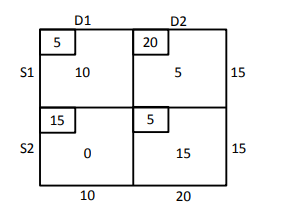
\includegraphics[width=0.75\columnwidth]{chapters/10/7/2/4/figs/fig.png}
 \end{center}
\caption{}
\label{fig:10/7/2/4Fig1}
\end{figure}
\fi

\item Find the position vector of the mid point of the vector joining the points $\vec{P}$(2, 3, 4)
and $\vec{Q}$(4, 1, –2).
\\
\solution
		\begin{enumerate}[label=\thesubsection.\arabic*,ref=\thesubsection.\theenumi]
\item Find the coordinates of the point which divides the join of $(-1,7) $ and $ (4,-3)$ in the ratio 2:3.
	\\
		\solution
	\input{chapters/10/7/2/1/section.tex}
\item Find the coordinates of the point $\vec{R}$ on the line segment joining the points $\vec{P}(-1,3)$ and $\vec{Q}(2,5)$ such that $PR=\frac{3}{5}PQ$.
\item Find the ratio in which the point $\vec{P}\brak{\frac{3}{4},\frac{5}{12}}$ divides the line segment joining the points $\vec{A}\brak{\frac{1}{2},\frac{3}{2}}$ and $ \vec{B}(2,-5)$.
\item Find the coordinates of the point which divides the line segment joining the points $(4,-3)$ and $(8,5)$ in the ratio $3:1$ internally.
\item Find the coordinates of the point $\vec{P}$ on $AD$ such that $AP : PD = 2 : 1$.
\item If the point $\vec{P} (2, 1)$ lies on the line segment joining points $\vec{A} (4, 2)$  and $ \vec{B} (8, 4)$,
then
\begin{enumerate}
	\item $AP =\frac{1}{3}{AB}$ 
\item ${AP}={PE}$
\item ${PB}=\frac{1}{3}{AB}$
\item${AP}=\frac{1}{2}{AB}$
 \end{enumerate}
\item Find the ratio in which the line segment joining the points $(-3,10)$  and  $(6,-8)$  is divided by $ (-1,6)$.
	\\
		\solution
	\input{chapters/10/7/2/4/section.tex}
\item Find the position vector of the mid point of the vector joining the points $\vec{P}$(2, 3, 4)
and $\vec{Q}$(4, 1, –2).
\\
\solution
		\input{chapters/12/10/2/16/section.tex}
\item Let $\vec{A}(4, 2), \vec{B}(6, 5)$  and $ \vec{C}(1, 4)$ be the vertices of $\triangle ABC$.
\begin{enumerate}
\item If $\vec{A}$ and  $\vec{B}$ are $(-2,-2)$ and  $(2,-4)$, respectively, find the coordinates of $\vec{P}$ such that $AP= \frac {3}{7}AB$  and $ \vec{P}$ lies on the line segment $AB$.
	\\
		\solution
	\input{chapters/10/7/2/8/section.tex}
\item Find the coordinates of the points which divide the line segment joining $A(-2,2)$  and  $\vec{B}(2,8)$ into four equal parts.
	\\
		\solution
	\input{chapters/10/7/2/9/section.tex}
\item In what ratio does the point $(-4,6)$ divide the line segment joining the points $\vec{A}(-6,0)$ and $\vec{B}(3,-8)$?
\item Given that $\vec{P}(3,2,-4), \vec{Q}(5,4,-6)$ and $\vec{R}(9,8,-10)$ are collinear. Find the ratio in which $\vec{Q}$ divides $PR$.
\item Points $\vec{A}(-6,10),\vec{B}(-4,6)$  and  $\vec{C}(3,-8)$ are collinear such that $AB=  \frac{2}{9}AC$.
\item The point which divides the line segment joining the points $\vec{P} (7, –6) $  and  $\vec{Q}(3, 4)$ in the 
ratio 1 : 2 internally lies in  which quadrant?
\item Find the coordinates of the points of trisection of the line segment joining $(4,-1)$  and  $(-2,3)$.
	\\
		\solution
	\input{chapters/10/7/2/2/section.tex}
\item Find the coordinates of the points which trisect the line segment joining the points $\vec{P}(4,2,-6)$ and $\vec{Q}(10,-16,6)$.
\item Find the coordinates of the points of trisection (i.e. points dividing to three equal parts) of the line segment joining the points $\vec{A}(2,-2)$ and $\vec{B}(-7,4)$.
\item Point $\vec{P}(5,-3)$ is one of the two points of trisection of line segment joining the points $\vec{A}(7,-2)$ and $\vec{B}(1,-5)$
\item Find the position vector of a point $\vec{R}$ which divides the line joining two points $\vec{P}$
and $\vec{Q}$ whose position vectors are $\hat{i}+2\hat{j}-\hat{k}$ and $-\hat{i}+\hat{j}+\hat{k}$ respectively, in the
ratio 2 : 1
\begin{enumerate}
    \item  internally
    \item  externally
\end{enumerate}
%\solution
%		\input{chapters/12/10/2/15/section.tex}
\item Find the coordinates of the point which divides the line segment joining the points which divides the line segment joining  the points $(-2,3,5)$ and $(1,-4,6)$ in the ratio 
\begin{enumerate}
\item $2:3$ internally,
\item $2:3$ externally
\end{enumerate}
\item Find the coordinates of the point which divides the line segment joining the points $(1,-2,3)$ and $(3,4,-5)$ in the ratio $2:3$
\begin{enumerate}
\item internally, and
\item externally
\end{enumerate}
\item Consider two points $\vec{P}$ and $\vec{Q}$ with position vectors $\overrightarrow{OP} = 3\overrightarrow{a}-2\overrightarrow{b}$ and $\overrightarrow{OQ}=\overrightarrow{a}+\overrightarrow{b}$. Find the position vector of a point $\vec{R}$ which divides the line joining $\vec{P}$ and $\vec{Q}$ in the ratio $2:1$, 
\begin{enumerate}
\item internally, and 
\item externally.
\end{enumerate}
\item The median from $\vec{A}$ meets $BC$ at $\vec{D}$. Find the coordinates of the point $\vec{D}$.
\item Find the coordinates of points $\vec{Q}$ and $\vec{R}$ on medians $BE$ and $CF$ respectively such that $BQ : QE = 2 : 1$  and  $CR : RF = 2 : 1$.
\item What do you observe?
\item If $\vec{A}, \vec{B}$ and $\vec{C}$  are the vertices of $\triangle ABC$, find the coordinates of the centroid of the triangle.
\end{enumerate}
\solution
	\input{chapters/10/7/4/7/section.tex}
\item If $\vec{P}(9a-2,-b)$ divides line segment joining $\vec{A}(3a+1,-3)$ and $\vec{B}(8a,5)$ in the ratio 3:1, find the values of $a$ and $b$.
\item Find the position vector of a point $\vec{R}$ which divides the line joining two points $\vec{P}$ and $\vec{Q}$ whose position vectors are $2\vec{a}+\vec{b}$ and $\vec{a}-3\vec{b}$ externally in the ratio $1:2$.
\item The position vector of the point which divides the join of points 2$\vec{a}$-3$\vec{b}$ $\text{and}$ $\vec{a}+\vec{b}$ in the ratio 3:1 is \rule{1cm}{0.1pt}.
\item If $\vec{a}$ and $\vec{b}$ are the postion vectors of $\vec{A}$ and $\vec{B}$, respectively, find the position vector of a point $\vec{C}$ in $BA$ produced such that $BC=1.5BA$.
\item Find the position vector of a point $\vec{R}$ which divides the line joining two points $\vec{P}$ and $\vec{Q}$ whose position vectors are $(2\vec{a}+\vec{b})$ and $(\vec{a}-3\vec{b})$
externally in the ratio 1 : 2. Also, show that $\vec{P}$ is the mid point of the line segment $RQ$.
\end{enumerate}

\item Let $\vec{A}(4, 2), \vec{B}(6, 5)$  and $ \vec{C}(1, 4)$ be the vertices of $\triangle ABC$.
\begin{enumerate}
\item If $\vec{A}$ and  $\vec{B}$ are $(-2,-2)$ and  $(2,-4)$, respectively, find the coordinates of $\vec{P}$ such that $AP= \frac {3}{7}AB$  and $ \vec{P}$ lies on the line segment $AB$.
	\\
		\solution
	\begin{enumerate}[label=\thesubsection.\arabic*,ref=\thesubsection.\theenumi]
\item Find the coordinates of the point which divides the join of $(-1,7) $ and $ (4,-3)$ in the ratio 2:3.
	\\
		\solution
	\input{chapters/10/7/2/1/section.tex}
\item Find the coordinates of the point $\vec{R}$ on the line segment joining the points $\vec{P}(-1,3)$ and $\vec{Q}(2,5)$ such that $PR=\frac{3}{5}PQ$.
\item Find the ratio in which the point $\vec{P}\brak{\frac{3}{4},\frac{5}{12}}$ divides the line segment joining the points $\vec{A}\brak{\frac{1}{2},\frac{3}{2}}$ and $ \vec{B}(2,-5)$.
\item Find the coordinates of the point which divides the line segment joining the points $(4,-3)$ and $(8,5)$ in the ratio $3:1$ internally.
\item Find the coordinates of the point $\vec{P}$ on $AD$ such that $AP : PD = 2 : 1$.
\item If the point $\vec{P} (2, 1)$ lies on the line segment joining points $\vec{A} (4, 2)$  and $ \vec{B} (8, 4)$,
then
\begin{enumerate}
	\item $AP =\frac{1}{3}{AB}$ 
\item ${AP}={PE}$
\item ${PB}=\frac{1}{3}{AB}$
\item${AP}=\frac{1}{2}{AB}$
 \end{enumerate}
\item Find the ratio in which the line segment joining the points $(-3,10)$  and  $(6,-8)$  is divided by $ (-1,6)$.
	\\
		\solution
	\input{chapters/10/7/2/4/section.tex}
\item Find the position vector of the mid point of the vector joining the points $\vec{P}$(2, 3, 4)
and $\vec{Q}$(4, 1, –2).
\\
\solution
		\input{chapters/12/10/2/16/section.tex}
\item Let $\vec{A}(4, 2), \vec{B}(6, 5)$  and $ \vec{C}(1, 4)$ be the vertices of $\triangle ABC$.
\begin{enumerate}
\item If $\vec{A}$ and  $\vec{B}$ are $(-2,-2)$ and  $(2,-4)$, respectively, find the coordinates of $\vec{P}$ such that $AP= \frac {3}{7}AB$  and $ \vec{P}$ lies on the line segment $AB$.
	\\
		\solution
	\input{chapters/10/7/2/8/section.tex}
\item Find the coordinates of the points which divide the line segment joining $A(-2,2)$  and  $\vec{B}(2,8)$ into four equal parts.
	\\
		\solution
	\input{chapters/10/7/2/9/section.tex}
\item In what ratio does the point $(-4,6)$ divide the line segment joining the points $\vec{A}(-6,0)$ and $\vec{B}(3,-8)$?
\item Given that $\vec{P}(3,2,-4), \vec{Q}(5,4,-6)$ and $\vec{R}(9,8,-10)$ are collinear. Find the ratio in which $\vec{Q}$ divides $PR$.
\item Points $\vec{A}(-6,10),\vec{B}(-4,6)$  and  $\vec{C}(3,-8)$ are collinear such that $AB=  \frac{2}{9}AC$.
\item The point which divides the line segment joining the points $\vec{P} (7, –6) $  and  $\vec{Q}(3, 4)$ in the 
ratio 1 : 2 internally lies in  which quadrant?
\item Find the coordinates of the points of trisection of the line segment joining $(4,-1)$  and  $(-2,3)$.
	\\
		\solution
	\input{chapters/10/7/2/2/section.tex}
\item Find the coordinates of the points which trisect the line segment joining the points $\vec{P}(4,2,-6)$ and $\vec{Q}(10,-16,6)$.
\item Find the coordinates of the points of trisection (i.e. points dividing to three equal parts) of the line segment joining the points $\vec{A}(2,-2)$ and $\vec{B}(-7,4)$.
\item Point $\vec{P}(5,-3)$ is one of the two points of trisection of line segment joining the points $\vec{A}(7,-2)$ and $\vec{B}(1,-5)$
\item Find the position vector of a point $\vec{R}$ which divides the line joining two points $\vec{P}$
and $\vec{Q}$ whose position vectors are $\hat{i}+2\hat{j}-\hat{k}$ and $-\hat{i}+\hat{j}+\hat{k}$ respectively, in the
ratio 2 : 1
\begin{enumerate}
    \item  internally
    \item  externally
\end{enumerate}
%\solution
%		\input{chapters/12/10/2/15/section.tex}
\item Find the coordinates of the point which divides the line segment joining the points which divides the line segment joining  the points $(-2,3,5)$ and $(1,-4,6)$ in the ratio 
\begin{enumerate}
\item $2:3$ internally,
\item $2:3$ externally
\end{enumerate}
\item Find the coordinates of the point which divides the line segment joining the points $(1,-2,3)$ and $(3,4,-5)$ in the ratio $2:3$
\begin{enumerate}
\item internally, and
\item externally
\end{enumerate}
\item Consider two points $\vec{P}$ and $\vec{Q}$ with position vectors $\overrightarrow{OP} = 3\overrightarrow{a}-2\overrightarrow{b}$ and $\overrightarrow{OQ}=\overrightarrow{a}+\overrightarrow{b}$. Find the position vector of a point $\vec{R}$ which divides the line joining $\vec{P}$ and $\vec{Q}$ in the ratio $2:1$, 
\begin{enumerate}
\item internally, and 
\item externally.
\end{enumerate}
\item The median from $\vec{A}$ meets $BC$ at $\vec{D}$. Find the coordinates of the point $\vec{D}$.
\item Find the coordinates of points $\vec{Q}$ and $\vec{R}$ on medians $BE$ and $CF$ respectively such that $BQ : QE = 2 : 1$  and  $CR : RF = 2 : 1$.
\item What do you observe?
\item If $\vec{A}, \vec{B}$ and $\vec{C}$  are the vertices of $\triangle ABC$, find the coordinates of the centroid of the triangle.
\end{enumerate}
\solution
	\input{chapters/10/7/4/7/section.tex}
\item If $\vec{P}(9a-2,-b)$ divides line segment joining $\vec{A}(3a+1,-3)$ and $\vec{B}(8a,5)$ in the ratio 3:1, find the values of $a$ and $b$.
\item Find the position vector of a point $\vec{R}$ which divides the line joining two points $\vec{P}$ and $\vec{Q}$ whose position vectors are $2\vec{a}+\vec{b}$ and $\vec{a}-3\vec{b}$ externally in the ratio $1:2$.
\item The position vector of the point which divides the join of points 2$\vec{a}$-3$\vec{b}$ $\text{and}$ $\vec{a}+\vec{b}$ in the ratio 3:1 is \rule{1cm}{0.1pt}.
\item If $\vec{a}$ and $\vec{b}$ are the postion vectors of $\vec{A}$ and $\vec{B}$, respectively, find the position vector of a point $\vec{C}$ in $BA$ produced such that $BC=1.5BA$.
\item Find the position vector of a point $\vec{R}$ which divides the line joining two points $\vec{P}$ and $\vec{Q}$ whose position vectors are $(2\vec{a}+\vec{b})$ and $(\vec{a}-3\vec{b})$
externally in the ratio 1 : 2. Also, show that $\vec{P}$ is the mid point of the line segment $RQ$.
\end{enumerate}

\item Find the coordinates of the points which divide the line segment joining $A(-2,2)$  and  $\vec{B}(2,8)$ into four equal parts.
	\\
		\solution
	\begin{enumerate}[label=\thesubsection.\arabic*,ref=\thesubsection.\theenumi]
\item Find the coordinates of the point which divides the join of $(-1,7) $ and $ (4,-3)$ in the ratio 2:3.
	\\
		\solution
	\input{chapters/10/7/2/1/section.tex}
\item Find the coordinates of the point $\vec{R}$ on the line segment joining the points $\vec{P}(-1,3)$ and $\vec{Q}(2,5)$ such that $PR=\frac{3}{5}PQ$.
\item Find the ratio in which the point $\vec{P}\brak{\frac{3}{4},\frac{5}{12}}$ divides the line segment joining the points $\vec{A}\brak{\frac{1}{2},\frac{3}{2}}$ and $ \vec{B}(2,-5)$.
\item Find the coordinates of the point which divides the line segment joining the points $(4,-3)$ and $(8,5)$ in the ratio $3:1$ internally.
\item Find the coordinates of the point $\vec{P}$ on $AD$ such that $AP : PD = 2 : 1$.
\item If the point $\vec{P} (2, 1)$ lies on the line segment joining points $\vec{A} (4, 2)$  and $ \vec{B} (8, 4)$,
then
\begin{enumerate}
	\item $AP =\frac{1}{3}{AB}$ 
\item ${AP}={PE}$
\item ${PB}=\frac{1}{3}{AB}$
\item${AP}=\frac{1}{2}{AB}$
 \end{enumerate}
\item Find the ratio in which the line segment joining the points $(-3,10)$  and  $(6,-8)$  is divided by $ (-1,6)$.
	\\
		\solution
	\input{chapters/10/7/2/4/section.tex}
\item Find the position vector of the mid point of the vector joining the points $\vec{P}$(2, 3, 4)
and $\vec{Q}$(4, 1, –2).
\\
\solution
		\input{chapters/12/10/2/16/section.tex}
\item Let $\vec{A}(4, 2), \vec{B}(6, 5)$  and $ \vec{C}(1, 4)$ be the vertices of $\triangle ABC$.
\begin{enumerate}
\item If $\vec{A}$ and  $\vec{B}$ are $(-2,-2)$ and  $(2,-4)$, respectively, find the coordinates of $\vec{P}$ such that $AP= \frac {3}{7}AB$  and $ \vec{P}$ lies on the line segment $AB$.
	\\
		\solution
	\input{chapters/10/7/2/8/section.tex}
\item Find the coordinates of the points which divide the line segment joining $A(-2,2)$  and  $\vec{B}(2,8)$ into four equal parts.
	\\
		\solution
	\input{chapters/10/7/2/9/section.tex}
\item In what ratio does the point $(-4,6)$ divide the line segment joining the points $\vec{A}(-6,0)$ and $\vec{B}(3,-8)$?
\item Given that $\vec{P}(3,2,-4), \vec{Q}(5,4,-6)$ and $\vec{R}(9,8,-10)$ are collinear. Find the ratio in which $\vec{Q}$ divides $PR$.
\item Points $\vec{A}(-6,10),\vec{B}(-4,6)$  and  $\vec{C}(3,-8)$ are collinear such that $AB=  \frac{2}{9}AC$.
\item The point which divides the line segment joining the points $\vec{P} (7, –6) $  and  $\vec{Q}(3, 4)$ in the 
ratio 1 : 2 internally lies in  which quadrant?
\item Find the coordinates of the points of trisection of the line segment joining $(4,-1)$  and  $(-2,3)$.
	\\
		\solution
	\input{chapters/10/7/2/2/section.tex}
\item Find the coordinates of the points which trisect the line segment joining the points $\vec{P}(4,2,-6)$ and $\vec{Q}(10,-16,6)$.
\item Find the coordinates of the points of trisection (i.e. points dividing to three equal parts) of the line segment joining the points $\vec{A}(2,-2)$ and $\vec{B}(-7,4)$.
\item Point $\vec{P}(5,-3)$ is one of the two points of trisection of line segment joining the points $\vec{A}(7,-2)$ and $\vec{B}(1,-5)$
\item Find the position vector of a point $\vec{R}$ which divides the line joining two points $\vec{P}$
and $\vec{Q}$ whose position vectors are $\hat{i}+2\hat{j}-\hat{k}$ and $-\hat{i}+\hat{j}+\hat{k}$ respectively, in the
ratio 2 : 1
\begin{enumerate}
    \item  internally
    \item  externally
\end{enumerate}
%\solution
%		\input{chapters/12/10/2/15/section.tex}
\item Find the coordinates of the point which divides the line segment joining the points which divides the line segment joining  the points $(-2,3,5)$ and $(1,-4,6)$ in the ratio 
\begin{enumerate}
\item $2:3$ internally,
\item $2:3$ externally
\end{enumerate}
\item Find the coordinates of the point which divides the line segment joining the points $(1,-2,3)$ and $(3,4,-5)$ in the ratio $2:3$
\begin{enumerate}
\item internally, and
\item externally
\end{enumerate}
\item Consider two points $\vec{P}$ and $\vec{Q}$ with position vectors $\overrightarrow{OP} = 3\overrightarrow{a}-2\overrightarrow{b}$ and $\overrightarrow{OQ}=\overrightarrow{a}+\overrightarrow{b}$. Find the position vector of a point $\vec{R}$ which divides the line joining $\vec{P}$ and $\vec{Q}$ in the ratio $2:1$, 
\begin{enumerate}
\item internally, and 
\item externally.
\end{enumerate}
\item The median from $\vec{A}$ meets $BC$ at $\vec{D}$. Find the coordinates of the point $\vec{D}$.
\item Find the coordinates of points $\vec{Q}$ and $\vec{R}$ on medians $BE$ and $CF$ respectively such that $BQ : QE = 2 : 1$  and  $CR : RF = 2 : 1$.
\item What do you observe?
\item If $\vec{A}, \vec{B}$ and $\vec{C}$  are the vertices of $\triangle ABC$, find the coordinates of the centroid of the triangle.
\end{enumerate}
\solution
	\input{chapters/10/7/4/7/section.tex}
\item If $\vec{P}(9a-2,-b)$ divides line segment joining $\vec{A}(3a+1,-3)$ and $\vec{B}(8a,5)$ in the ratio 3:1, find the values of $a$ and $b$.
\item Find the position vector of a point $\vec{R}$ which divides the line joining two points $\vec{P}$ and $\vec{Q}$ whose position vectors are $2\vec{a}+\vec{b}$ and $\vec{a}-3\vec{b}$ externally in the ratio $1:2$.
\item The position vector of the point which divides the join of points 2$\vec{a}$-3$\vec{b}$ $\text{and}$ $\vec{a}+\vec{b}$ in the ratio 3:1 is \rule{1cm}{0.1pt}.
\item If $\vec{a}$ and $\vec{b}$ are the postion vectors of $\vec{A}$ and $\vec{B}$, respectively, find the position vector of a point $\vec{C}$ in $BA$ produced such that $BC=1.5BA$.
\item Find the position vector of a point $\vec{R}$ which divides the line joining two points $\vec{P}$ and $\vec{Q}$ whose position vectors are $(2\vec{a}+\vec{b})$ and $(\vec{a}-3\vec{b})$
externally in the ratio 1 : 2. Also, show that $\vec{P}$ is the mid point of the line segment $RQ$.
\end{enumerate}

\item In what ratio does the point $(-4,6)$ divide the line segment joining the points $\vec{A}(-6,0)$ and $\vec{B}(3,-8)$?
\item Given that $\vec{P}(3,2,-4), \vec{Q}(5,4,-6)$ and $\vec{R}(9,8,-10)$ are collinear. Find the ratio in which $\vec{Q}$ divides $PR$.
\item Points $\vec{A}(-6,10),\vec{B}(-4,6)$  and  $\vec{C}(3,-8)$ are collinear such that $AB=  \frac{2}{9}AC$.
\item The point which divides the line segment joining the points $\vec{P} (7, –6) $  and  $\vec{Q}(3, 4)$ in the 
ratio 1 : 2 internally lies in  which quadrant?
\item Find the coordinates of the points of trisection of the line segment joining $(4,-1)$  and  $(-2,3)$.
	\\
		\solution
	Using section formula,
\begin{align}
\vec{R}=\frac{1}{1+\frac{1}{2}}\brak{\myvec{4\\-1}+\frac{1}{2}\myvec{-2\\3}}
=\myvec{2\\ \frac{1}{3}}\\
\vec{S}=\frac{1}{1+\frac{2}{1}}\brak{\myvec{4\\-1}+\frac{2}{1}\myvec{-2\\3}}
=\myvec{0\\ \frac{5}{3}}
\end{align}
which are the desired points of trisection.
\iffalse
See
		\figref{fig:chapters/10/7/2/2/Figure}
\begin{figure}[H]
\centering
\includegraphics[width=0.75\columnwidth]{chapters/10/7/2/2/figs/dj.pdf}
\caption{}
		\label{fig:chapters/10/7/2/2/Figure}
\end{figure}
\fi

\item Find the coordinates of the points which trisect the line segment joining the points $\vec{P}(4,2,-6)$ and $\vec{Q}(10,-16,6)$.
\item Find the coordinates of the points of trisection (i.e. points dividing to three equal parts) of the line segment joining the points $\vec{A}(2,-2)$ and $\vec{B}(-7,4)$.
\item Point $\vec{P}(5,-3)$ is one of the two points of trisection of line segment joining the points $\vec{A}(7,-2)$ and $\vec{B}(1,-5)$
\item Find the position vector of a point $\vec{R}$ which divides the line joining two points $\vec{P}$
and $\vec{Q}$ whose position vectors are $\hat{i}+2\hat{j}-\hat{k}$ and $-\hat{i}+\hat{j}+\hat{k}$ respectively, in the
ratio 2 : 1
\begin{enumerate}
    \item  internally
    \item  externally
\end{enumerate}
%\solution
%		\begin{enumerate}[label=\thesubsection.\arabic*,ref=\thesubsection.\theenumi]
\item Find the coordinates of the point which divides the join of $(-1,7) $ and $ (4,-3)$ in the ratio 2:3.
	\\
		\solution
	\input{chapters/10/7/2/1/section.tex}
\item Find the coordinates of the point $\vec{R}$ on the line segment joining the points $\vec{P}(-1,3)$ and $\vec{Q}(2,5)$ such that $PR=\frac{3}{5}PQ$.
\item Find the ratio in which the point $\vec{P}\brak{\frac{3}{4},\frac{5}{12}}$ divides the line segment joining the points $\vec{A}\brak{\frac{1}{2},\frac{3}{2}}$ and $ \vec{B}(2,-5)$.
\item Find the coordinates of the point which divides the line segment joining the points $(4,-3)$ and $(8,5)$ in the ratio $3:1$ internally.
\item Find the coordinates of the point $\vec{P}$ on $AD$ such that $AP : PD = 2 : 1$.
\item If the point $\vec{P} (2, 1)$ lies on the line segment joining points $\vec{A} (4, 2)$  and $ \vec{B} (8, 4)$,
then
\begin{enumerate}
	\item $AP =\frac{1}{3}{AB}$ 
\item ${AP}={PE}$
\item ${PB}=\frac{1}{3}{AB}$
\item${AP}=\frac{1}{2}{AB}$
 \end{enumerate}
\item Find the ratio in which the line segment joining the points $(-3,10)$  and  $(6,-8)$  is divided by $ (-1,6)$.
	\\
		\solution
	\input{chapters/10/7/2/4/section.tex}
\item Find the position vector of the mid point of the vector joining the points $\vec{P}$(2, 3, 4)
and $\vec{Q}$(4, 1, –2).
\\
\solution
		\input{chapters/12/10/2/16/section.tex}
\item Let $\vec{A}(4, 2), \vec{B}(6, 5)$  and $ \vec{C}(1, 4)$ be the vertices of $\triangle ABC$.
\begin{enumerate}
\item If $\vec{A}$ and  $\vec{B}$ are $(-2,-2)$ and  $(2,-4)$, respectively, find the coordinates of $\vec{P}$ such that $AP= \frac {3}{7}AB$  and $ \vec{P}$ lies on the line segment $AB$.
	\\
		\solution
	\input{chapters/10/7/2/8/section.tex}
\item Find the coordinates of the points which divide the line segment joining $A(-2,2)$  and  $\vec{B}(2,8)$ into four equal parts.
	\\
		\solution
	\input{chapters/10/7/2/9/section.tex}
\item In what ratio does the point $(-4,6)$ divide the line segment joining the points $\vec{A}(-6,0)$ and $\vec{B}(3,-8)$?
\item Given that $\vec{P}(3,2,-4), \vec{Q}(5,4,-6)$ and $\vec{R}(9,8,-10)$ are collinear. Find the ratio in which $\vec{Q}$ divides $PR$.
\item Points $\vec{A}(-6,10),\vec{B}(-4,6)$  and  $\vec{C}(3,-8)$ are collinear such that $AB=  \frac{2}{9}AC$.
\item The point which divides the line segment joining the points $\vec{P} (7, –6) $  and  $\vec{Q}(3, 4)$ in the 
ratio 1 : 2 internally lies in  which quadrant?
\item Find the coordinates of the points of trisection of the line segment joining $(4,-1)$  and  $(-2,3)$.
	\\
		\solution
	\input{chapters/10/7/2/2/section.tex}
\item Find the coordinates of the points which trisect the line segment joining the points $\vec{P}(4,2,-6)$ and $\vec{Q}(10,-16,6)$.
\item Find the coordinates of the points of trisection (i.e. points dividing to three equal parts) of the line segment joining the points $\vec{A}(2,-2)$ and $\vec{B}(-7,4)$.
\item Point $\vec{P}(5,-3)$ is one of the two points of trisection of line segment joining the points $\vec{A}(7,-2)$ and $\vec{B}(1,-5)$
\item Find the position vector of a point $\vec{R}$ which divides the line joining two points $\vec{P}$
and $\vec{Q}$ whose position vectors are $\hat{i}+2\hat{j}-\hat{k}$ and $-\hat{i}+\hat{j}+\hat{k}$ respectively, in the
ratio 2 : 1
\begin{enumerate}
    \item  internally
    \item  externally
\end{enumerate}
%\solution
%		\input{chapters/12/10/2/15/section.tex}
\item Find the coordinates of the point which divides the line segment joining the points which divides the line segment joining  the points $(-2,3,5)$ and $(1,-4,6)$ in the ratio 
\begin{enumerate}
\item $2:3$ internally,
\item $2:3$ externally
\end{enumerate}
\item Find the coordinates of the point which divides the line segment joining the points $(1,-2,3)$ and $(3,4,-5)$ in the ratio $2:3$
\begin{enumerate}
\item internally, and
\item externally
\end{enumerate}
\item Consider two points $\vec{P}$ and $\vec{Q}$ with position vectors $\overrightarrow{OP} = 3\overrightarrow{a}-2\overrightarrow{b}$ and $\overrightarrow{OQ}=\overrightarrow{a}+\overrightarrow{b}$. Find the position vector of a point $\vec{R}$ which divides the line joining $\vec{P}$ and $\vec{Q}$ in the ratio $2:1$, 
\begin{enumerate}
\item internally, and 
\item externally.
\end{enumerate}
\item The median from $\vec{A}$ meets $BC$ at $\vec{D}$. Find the coordinates of the point $\vec{D}$.
\item Find the coordinates of points $\vec{Q}$ and $\vec{R}$ on medians $BE$ and $CF$ respectively such that $BQ : QE = 2 : 1$  and  $CR : RF = 2 : 1$.
\item What do you observe?
\item If $\vec{A}, \vec{B}$ and $\vec{C}$  are the vertices of $\triangle ABC$, find the coordinates of the centroid of the triangle.
\end{enumerate}
\solution
	\input{chapters/10/7/4/7/section.tex}
\item If $\vec{P}(9a-2,-b)$ divides line segment joining $\vec{A}(3a+1,-3)$ and $\vec{B}(8a,5)$ in the ratio 3:1, find the values of $a$ and $b$.
\item Find the position vector of a point $\vec{R}$ which divides the line joining two points $\vec{P}$ and $\vec{Q}$ whose position vectors are $2\vec{a}+\vec{b}$ and $\vec{a}-3\vec{b}$ externally in the ratio $1:2$.
\item The position vector of the point which divides the join of points 2$\vec{a}$-3$\vec{b}$ $\text{and}$ $\vec{a}+\vec{b}$ in the ratio 3:1 is \rule{1cm}{0.1pt}.
\item If $\vec{a}$ and $\vec{b}$ are the postion vectors of $\vec{A}$ and $\vec{B}$, respectively, find the position vector of a point $\vec{C}$ in $BA$ produced such that $BC=1.5BA$.
\item Find the position vector of a point $\vec{R}$ which divides the line joining two points $\vec{P}$ and $\vec{Q}$ whose position vectors are $(2\vec{a}+\vec{b})$ and $(\vec{a}-3\vec{b})$
externally in the ratio 1 : 2. Also, show that $\vec{P}$ is the mid point of the line segment $RQ$.
\end{enumerate}

\item Find the coordinates of the point which divides the line segment joining the points which divides the line segment joining  the points $(-2,3,5)$ and $(1,-4,6)$ in the ratio 
\begin{enumerate}
\item $2:3$ internally,
\item $2:3$ externally
\end{enumerate}
\item Find the coordinates of the point which divides the line segment joining the points $(1,-2,3)$ and $(3,4,-5)$ in the ratio $2:3$
\begin{enumerate}
\item internally, and
\item externally
\end{enumerate}
\item Consider two points $\vec{P}$ and $\vec{Q}$ with position vectors $\overrightarrow{OP} = 3\overrightarrow{a}-2\overrightarrow{b}$ and $\overrightarrow{OQ}=\overrightarrow{a}+\overrightarrow{b}$. Find the position vector of a point $\vec{R}$ which divides the line joining $\vec{P}$ and $\vec{Q}$ in the ratio $2:1$, 
\begin{enumerate}
\item internally, and 
\item externally.
\end{enumerate}
\item The median from $\vec{A}$ meets $BC$ at $\vec{D}$. Find the coordinates of the point $\vec{D}$.
\item Find the coordinates of points $\vec{Q}$ and $\vec{R}$ on medians $BE$ and $CF$ respectively such that $BQ : QE = 2 : 1$  and  $CR : RF = 2 : 1$.
\item What do you observe?
\item If $\vec{A}, \vec{B}$ and $\vec{C}$  are the vertices of $\triangle ABC$, find the coordinates of the centroid of the triangle.
\end{enumerate}
\solution
	\begin{enumerate}[label=\thesubsection.\arabic*,ref=\thesubsection.\theenumi]
\item Find the coordinates of the point which divides the join of $(-1,7) $ and $ (4,-3)$ in the ratio 2:3.
	\\
		\solution
	\input{chapters/10/7/2/1/section.tex}
\item Find the coordinates of the point $\vec{R}$ on the line segment joining the points $\vec{P}(-1,3)$ and $\vec{Q}(2,5)$ such that $PR=\frac{3}{5}PQ$.
\item Find the ratio in which the point $\vec{P}\brak{\frac{3}{4},\frac{5}{12}}$ divides the line segment joining the points $\vec{A}\brak{\frac{1}{2},\frac{3}{2}}$ and $ \vec{B}(2,-5)$.
\item Find the coordinates of the point which divides the line segment joining the points $(4,-3)$ and $(8,5)$ in the ratio $3:1$ internally.
\item Find the coordinates of the point $\vec{P}$ on $AD$ such that $AP : PD = 2 : 1$.
\item If the point $\vec{P} (2, 1)$ lies on the line segment joining points $\vec{A} (4, 2)$  and $ \vec{B} (8, 4)$,
then
\begin{enumerate}
	\item $AP =\frac{1}{3}{AB}$ 
\item ${AP}={PE}$
\item ${PB}=\frac{1}{3}{AB}$
\item${AP}=\frac{1}{2}{AB}$
 \end{enumerate}
\item Find the ratio in which the line segment joining the points $(-3,10)$  and  $(6,-8)$  is divided by $ (-1,6)$.
	\\
		\solution
	\input{chapters/10/7/2/4/section.tex}
\item Find the position vector of the mid point of the vector joining the points $\vec{P}$(2, 3, 4)
and $\vec{Q}$(4, 1, –2).
\\
\solution
		\input{chapters/12/10/2/16/section.tex}
\item Let $\vec{A}(4, 2), \vec{B}(6, 5)$  and $ \vec{C}(1, 4)$ be the vertices of $\triangle ABC$.
\begin{enumerate}
\item If $\vec{A}$ and  $\vec{B}$ are $(-2,-2)$ and  $(2,-4)$, respectively, find the coordinates of $\vec{P}$ such that $AP= \frac {3}{7}AB$  and $ \vec{P}$ lies on the line segment $AB$.
	\\
		\solution
	\input{chapters/10/7/2/8/section.tex}
\item Find the coordinates of the points which divide the line segment joining $A(-2,2)$  and  $\vec{B}(2,8)$ into four equal parts.
	\\
		\solution
	\input{chapters/10/7/2/9/section.tex}
\item In what ratio does the point $(-4,6)$ divide the line segment joining the points $\vec{A}(-6,0)$ and $\vec{B}(3,-8)$?
\item Given that $\vec{P}(3,2,-4), \vec{Q}(5,4,-6)$ and $\vec{R}(9,8,-10)$ are collinear. Find the ratio in which $\vec{Q}$ divides $PR$.
\item Points $\vec{A}(-6,10),\vec{B}(-4,6)$  and  $\vec{C}(3,-8)$ are collinear such that $AB=  \frac{2}{9}AC$.
\item The point which divides the line segment joining the points $\vec{P} (7, –6) $  and  $\vec{Q}(3, 4)$ in the 
ratio 1 : 2 internally lies in  which quadrant?
\item Find the coordinates of the points of trisection of the line segment joining $(4,-1)$  and  $(-2,3)$.
	\\
		\solution
	\input{chapters/10/7/2/2/section.tex}
\item Find the coordinates of the points which trisect the line segment joining the points $\vec{P}(4,2,-6)$ and $\vec{Q}(10,-16,6)$.
\item Find the coordinates of the points of trisection (i.e. points dividing to three equal parts) of the line segment joining the points $\vec{A}(2,-2)$ and $\vec{B}(-7,4)$.
\item Point $\vec{P}(5,-3)$ is one of the two points of trisection of line segment joining the points $\vec{A}(7,-2)$ and $\vec{B}(1,-5)$
\item Find the position vector of a point $\vec{R}$ which divides the line joining two points $\vec{P}$
and $\vec{Q}$ whose position vectors are $\hat{i}+2\hat{j}-\hat{k}$ and $-\hat{i}+\hat{j}+\hat{k}$ respectively, in the
ratio 2 : 1
\begin{enumerate}
    \item  internally
    \item  externally
\end{enumerate}
%\solution
%		\input{chapters/12/10/2/15/section.tex}
\item Find the coordinates of the point which divides the line segment joining the points which divides the line segment joining  the points $(-2,3,5)$ and $(1,-4,6)$ in the ratio 
\begin{enumerate}
\item $2:3$ internally,
\item $2:3$ externally
\end{enumerate}
\item Find the coordinates of the point which divides the line segment joining the points $(1,-2,3)$ and $(3,4,-5)$ in the ratio $2:3$
\begin{enumerate}
\item internally, and
\item externally
\end{enumerate}
\item Consider two points $\vec{P}$ and $\vec{Q}$ with position vectors $\overrightarrow{OP} = 3\overrightarrow{a}-2\overrightarrow{b}$ and $\overrightarrow{OQ}=\overrightarrow{a}+\overrightarrow{b}$. Find the position vector of a point $\vec{R}$ which divides the line joining $\vec{P}$ and $\vec{Q}$ in the ratio $2:1$, 
\begin{enumerate}
\item internally, and 
\item externally.
\end{enumerate}
\item The median from $\vec{A}$ meets $BC$ at $\vec{D}$. Find the coordinates of the point $\vec{D}$.
\item Find the coordinates of points $\vec{Q}$ and $\vec{R}$ on medians $BE$ and $CF$ respectively such that $BQ : QE = 2 : 1$  and  $CR : RF = 2 : 1$.
\item What do you observe?
\item If $\vec{A}, \vec{B}$ and $\vec{C}$  are the vertices of $\triangle ABC$, find the coordinates of the centroid of the triangle.
\end{enumerate}
\solution
	\input{chapters/10/7/4/7/section.tex}
\item If $\vec{P}(9a-2,-b)$ divides line segment joining $\vec{A}(3a+1,-3)$ and $\vec{B}(8a,5)$ in the ratio 3:1, find the values of $a$ and $b$.
\item Find the position vector of a point $\vec{R}$ which divides the line joining two points $\vec{P}$ and $\vec{Q}$ whose position vectors are $2\vec{a}+\vec{b}$ and $\vec{a}-3\vec{b}$ externally in the ratio $1:2$.
\item The position vector of the point which divides the join of points 2$\vec{a}$-3$\vec{b}$ $\text{and}$ $\vec{a}+\vec{b}$ in the ratio 3:1 is \rule{1cm}{0.1pt}.
\item If $\vec{a}$ and $\vec{b}$ are the postion vectors of $\vec{A}$ and $\vec{B}$, respectively, find the position vector of a point $\vec{C}$ in $BA$ produced such that $BC=1.5BA$.
\item Find the position vector of a point $\vec{R}$ which divides the line joining two points $\vec{P}$ and $\vec{Q}$ whose position vectors are $(2\vec{a}+\vec{b})$ and $(\vec{a}-3\vec{b})$
externally in the ratio 1 : 2. Also, show that $\vec{P}$ is the mid point of the line segment $RQ$.
\end{enumerate}

\item If $\vec{P}(9a-2,-b)$ divides line segment joining $\vec{A}(3a+1,-3)$ and $\vec{B}(8a,5)$ in the ratio 3:1, find the values of $a$ and $b$.
\item Find the position vector of a point $\vec{R}$ which divides the line joining two points $\vec{P}$ and $\vec{Q}$ whose position vectors are $2\vec{a}+\vec{b}$ and $\vec{a}-3\vec{b}$ externally in the ratio $1:2$.
\item The position vector of the point which divides the join of points 2$\vec{a}$-3$\vec{b}$ $\text{and}$ $\vec{a}+\vec{b}$ in the ratio 3:1 is \rule{1cm}{0.1pt}.
\item If $\vec{a}$ and $\vec{b}$ are the postion vectors of $\vec{A}$ and $\vec{B}$, respectively, find the position vector of a point $\vec{C}$ in $BA$ produced such that $BC=1.5BA$.
\item Find the position vector of a point $\vec{R}$ which divides the line joining two points $\vec{P}$ and $\vec{Q}$ whose position vectors are $(2\vec{a}+\vec{b})$ and $(\vec{a}-3\vec{b})$
externally in the ratio 1 : 2. Also, show that $\vec{P}$ is the mid point of the line segment $RQ$.
\end{enumerate}

\item If $\vec{P}(9a-2,-b)$ divides line segment joining $\vec{A}(3a+1,-3)$ and $\vec{B}(8a,5)$ in the ratio 3:1, find the values of $a$ and $b$.
\item Find the position vector of a point $\vec{R}$ which divides the line joining two points $\vec{P}$ and $\vec{Q}$ whose position vectors are $2\vec{a}+\vec{b}$ and $\vec{a}-3\vec{b}$ externally in the ratio $1:2$.
\item The position vector of the point which divides the join of points 2$\vec{a}$-3$\vec{b}$ $\text{and}$ $\vec{a}+\vec{b}$ in the ratio 3:1 is \rule{1cm}{0.1pt}.
\item If $\vec{a}$ and $\vec{b}$ are the postion vectors of $\vec{A}$ and $\vec{B}$, respectively, find the position vector of a point $\vec{C}$ in $BA$ produced such that $BC=1.5BA$.
\item Find the position vector of a point $\vec{R}$ which divides the line joining two points $\vec{P}$ and $\vec{Q}$ whose position vectors are $(2\vec{a}+\vec{b})$ and $(\vec{a}-3\vec{b})$
externally in the ratio 1 : 2. Also, show that $\vec{P}$ is the mid point of the line segment $RQ$.
\end{enumerate}

\item If the area of triangle is 35 square units with vertices $(2,6), (5,-4)$ and $(k,4)$. Then $k$ is \rule{1cm}{0.1pt}.
\item Find values of $k$ if area of triangle is 4 square units and vertices are
\begin{enumerate}
\item $(k,0), (4,0), (0,2)$
\item $(-2,0), (0,4), (0,k)$
\end{enumerate}
\item Find the area of the triangle whose vertices are $(1,-1), (-4,6)$ and $(-3,5)$.
\item Find area of the triangle with vertices at the point given in each of the following:
\begin{enumerate}
\item $(1,0), (6,0), (4,3)$
\item $(2.7), (1,1), (10,8)$
\item $(-2,-3), (3,2), (-1,8)$
\end{enumerate}
\item Find the area of region bounded by the triangle whose vertices are $(-1, 1), (0, 5)$ and $(3, 2)$.
\item The value of $\hat{i}\cdot(\hat{j}\times\hat{k})+\hat{j}\cdot(\hat{i}\times\hat{k})+\hat{k}\cdot(\hat{i}\times\hat{j})$ is \rule{1cm}{0.1pt}.
\item The value of $\hat{i}\cdot (\hat{j}\times\hat{k})+\hat{j}\cdot (\hat{i}\times\hat{k})+\hat{k}\cdot (\hat{i}\times\hat{j})$ is \rule{1cm}{0.1pt}.

\item The vector from origin to the points $\vec{A}$ and $\vec{B}$ are $\vec{a}$ = $2\hat{i}-3\hat{j}+2\hat{k}$ and  $\vec{b}$ = $2\hat{i}+3\hat{j}+\hat{k}$, respectively, then the area of $\triangle {OAB}$ is \rule{1cm}{0.1pt}.
\item If $\vec{a} = \hat{i}+\hat{j}+\hat{k}$ and $\vec{b} = \hat{j}-\hat{k}$, find a vector $\vec{c}$ such that $\vec{a}\times\vec{c} = \vec{b}$ and $\vec{a}\cdot \vec{c}$ = 3.
%
\item The area of the quadrilateral ABCD, where A$(0,4,1)$, B$(2,3,-1)$, C$(4,5,0)$ and D$(2,6,2)$, is equal to \rule{1cm}{0.1pt}.
    \item Draw a quadrilateral in the Cartesian plane, whose vertices are 
    \begin{align}
        \vec{A} = \myvec{-4\\5},\, \vec{B} = \myvec{0\\7},\, 
        \vec{C} = \myvec{5\\-5},\, \vec{D} = \myvec{-4\\-2}.
    \end{align}
    Also, find its area.
\label{chapters/11/10/1/1}
   \\ 
    \solution 
\begin{enumerate}[label=\thesubsection.\arabic*, ref=\thesubsection.\theenumi]
\item The area of a triangle formed by vertices $\vec{O}$,  $\vec{A}$ and $\vec{B}$,  where $\overrightarrow{OA}= \hat{i}+2 \hat{j}+3\hat{k}$ and $\overrightarrow{OB}= -3\hat{i} - 2\hat{j} + \hat{k}$ is
\hfill (12,  2020)
    \item  Find the area of the triangle whose vertices are $(-1,  1)$,  $(0,  5)$,  and $(3,  2)$.
    \hfill (12,  2023)
    \item If $\overrightarrow{a}$ and $\overrightarrow{b}$ are two vectors such that
    \begin{align}
        \overrightarrow{a} = \hat{i} - \hat{j} + \hat{k}
    \end{align}
    and
    \begin{align}
        \overrightarrow{b} = 2\hat{i} - \hat{j} - 3\hat{k}, 
    \end{align}
    then find the vector $\overrightarrow{c}$,  given that
    \begin{align}
        \overrightarrow{a} \times \overrightarrow{c} = \overrightarrow{b}
    \end{align}
    and
    \begin{align}
        \overrightarrow{a} \cdot \overrightarrow{c} = 4.
    \end{align}
    \hfill (12,  2023)
    \item If
    \begin{align}
        \overrightarrow{a} = 2\hat{i} + \hat{j} + 3\hat{k}, 
    \end{align}
    \begin{align}
        \overrightarrow{b} = -\hat{i} + 2\hat{j} + \hat{k}, 
    \end{align}
    and
    \begin{align}
        \overrightarrow{c} = 3\hat{i} + \hat{j} + 2\hat{k}, 
    \end{align}
    then find $\overrightarrow{a} \cdot (\overrightarrow{b} \times \overrightarrow{c})$.
    \hfill (12,  2023)
    \item Find the area of the triangle with vertices $\vec{A}(-1,  0,  -2)$,  $\vec{B}(0,  2,  1)$,  and $\vec{C}(-1,  4,  1)$.
    \hfill (12,  2023)

    \item Find the area of the triangle with vertices $(2,  0)$,  $(4,  5)$,  and $(1,  4)$.
    \hfill (12,  2023)
    \item Find the area of the quadrilateral $ABCD$ whose vertices are $\vec{A}(-4,  -3)$,  $\vec{B}(3,  -1)$,  $\vec{C}(0,  5)$,  and $\vec{D}(-4,  2)$.
    \hfill (10,  2022)
	\item Find $|\overrightarrow{a} \times \overrightarrow{b}|$,  if $\overrightarrow{a} = 2\hat{i} + \hat{j} + 3\hat{k}$ and $\overrightarrow{b} = 3\hat{i} + 5\hat{j} - 2\hat{k}$. \hfill (12,  2019)
	\item Find the area of the triangle whose vertices are $(1,  0)$,  $(2,  2)$,  and $(3,  1)$. \hfill (12,  2019)
	\item Find the area of the triangle whose vertices are $(-1,  1)$,  $(0,  5)$,  and $(3,  2)$. \hfill (12,  2019)
\item Find the area of a triangle whose vertices are $(1,  -1)$,  $(-4,  6)$,  and $(-3,  -5)$.

	\hfill (10,  2019)
\item Find the area of the triangle formed by joining the midpoints of the sides of the triangle $ABC$,  whose vertices are $\vec{A}(0,  -1)$,  $\vec{B}(2,  1)$,  and $\vec{C}(0,  3)$. \hfill (10,  2019)
    \item Given vertices $\vec{A}(-5, 7)$,  $\vec{B}(-4, -5)$,  $\vec{C}(-1, -6)$,  and $\vec{D}(4, 5)$ of a quadrilateral. Find the area of quadrilateral $ABCD$. \hfill (10,  2018)
\item If $\theta$ is the angle between the two vectors $\hat{i} - 2\hat{j} + 3\hat{k}$ and $3\hat{i} - 2\hat{j} + \hat{k}$, find $\sin \theta$.

	\hfill (12,  2018)
\item Find the volume of a cuboid whose edges are given by $-3\hat{i}+7\hat{j}+5\hat{k}$, $-5\hat{i}+7\hat{j}-3\hat{k}$ and $7\hat{i}-5\hat{j}-3\hat{k}$.

\hfill (12,  2018) 
\item Find $\abs{\overrightarrow{a} \times \overrightarrow{b}}$,  if $\overrightarrow{a}=2\hat{i}+\hat{j}+3\hat{k}$ and $\overrightarrow{b}=3\hat{i}+5\hat{j}-2\hat{k}$.
\hfill (12,  2018) 
    \item Show that the points $\vec{A} = 2\hat{i} - \hat{j} + \hat{k}$,  $\vec{B} = \hat{i} - 3\hat{j} - 5\hat{k}$,  and $\vec{C} = 3\hat{i} - 4\hat{j} - 4\hat{k}$ respectively,  are the vertices of a right-angled triangle. Hence, find the area of the triangle.

	    \hfill (12,  2017)
    \item The vertices of $\triangle ABC$ are $\vec{A} \myvec{4,  6}$,  $\vec{B} \myvec{1,  5}$,  and $\vec{C} \myvec{7,  2}$. A line-segment $DE$ is drawn to intersect the sides $AB$ and $AC$ at $\vec{D}$ and $\vec{E}$ respectively such that $\frac{AD}{AB} = \frac{AE}{AC} = \frac{1}{3}$. Calculate the area of $\triangle ADE$ and compare it with the area of $\triangle ABC$. \hfill (10,  2016)
\item Find $\lambda$ and $\mu$ if
      \begin{align*}
          \myvec{\hat{i} + 3\hat{j} + 9\hat{k}} \times \myvec{3\hat{i} - \lambda \hat{j} + \mu \hat{k}} = \overrightarrow{0}.
      \end{align*}
      \hfill (12,  2016)
\item The two adjacent sides of a parallelogram are $2\hat{i}-4\hat{j}-5\hat{k}$ and $2\hat{i}+2\hat{j}+3\hat{k}$. Find the two unit vectors parallel to its diagonals. Using the diagonal vectorsFind the area of the parallelogram. \hfill (12,  2016)
\item Find the values of $k$ so that the area of the triangle with vertices $\brak{1,  -1}$,  $\brak{-4,  2k}$,  and $\brak{-k,  -5}$ is $24$ sq. units. \hfill (10,  2015)
\item The area of a triangle whose vertices are $\brak{5, 0}$,  $\brak{8, 0}$ and $\brak{8, 4}$ $\brak{\text{in sq. units}}$ is

\hfill (10,  2012)
\item For what value of $k$,  $\brak{ k > 0}$,  is the area of the triangle with vertices $\brak{-2, 5}$,  $\brak{k, -4}$,  and $\brak{2k+1, 10}$ equal to $52$ sq. units? 
\hfill (10,  2012)

\item If the vertices of a triangle are $\brak{1, -3}$,  $\brak{4, p}$ and $\brak{-9, 7}$ and its area is $15$ sq. units. Find the value$\brak{\text{s}}$ of $p$. 
\hfill (10,  2012)

\item Find the area of quadrilateral $ABCD$ whose vertices are $\vec{A}\brak{-3, -1}$,  $\vec{B}\brak{-2, -4}$,  $\vec{C}\brak{4, -1}$ and $\vec{D}\brak{3, 4}$.
\hfill (10,  2012)
\item Find the area of the quadrilateral $ABCD$,  whose vertices are $\vec{A}(-3,  -1)$,  $\vec{B}(-2,  -4)$,  $\vec{C}(4,  -1)$,  and $\vec{D}(3,  4)$.
\hfill (10,  2011)
\item Find the area of triangle $ABC$,  whose vertices are $\vec{A}\brak{2,  5}$,  $\vec{B}\brak{4,  7}$ and $\vec{C}\brak{6,  2}$.
\hfill (12,  2018)
\item Find the area of the triangle whose vertices are $\brak{2, 3}, \brak{3, 5}$ and $\brak{4, 4}$
\hfill (12,  2018)
\item The area of a triangle formed by vertices $\vec{O}$,  $\vec{A}$ and $\vec{B}$,  where $\overrightarrow{OA}= \hat{i}+2 \hat{j}+3\hat{k}$ and $\overrightarrow{OB}= -3\hat{i} - 2\hat{j} + \hat{k}$ is
\hfill (12,  2020)
\item Find the value of $k$ so that the area of triangle $ABC$ with $\vec{A}\brak{k + 1,  1}$,  $\vec{B}\brak{4,  -3}$ and $\vec{C}\brak{7,  -k}$ is $6$ square units.
\hfill (10,  2019)
\item Find the area of triangle $ABC$,  whose vertices are $\vec{A}\brak{2,  5}$,  $\vec{B}\brak{4,  7}$ and $\vec{C}\brak{6,  2}$.
\hfill (12,  2018)
\item Find the area of the triangle whose vertices are $\brak{2, 3}, \brak{3, 5}$ and $\brak{4, 4}$
\hfill (12,  2018)
\item 
Find the value of $p$ if 
$$(2\hat{i} + 6\hat{j} + 27\hat{k}) \times (\hat{i} + 3\hat{j} + p\hat{k}) = \vec{0}.$$
\hfill	(10, 2009)

\end{enumerate}

\item The area of a triangle with vertices $\vec{A}(3, 0), \vec{B}(7, 0)$ and  $\vec{C}(8, 4)$ is \rule{1cm}{0.1pt}.
\item Find the area of the triangle whose vertices are $(-8,4),(-6,6)$ and $(-3,9)$.
\item If $\vec{D}\brak{\frac{-1}{2},\frac{5}{2}},\vec{E}(7,3)$ and $\vec{F}\brak{\frac{7}{2},\frac{7}{2}}$ are the midpoints of sides of $\triangle ABC$, find the area of the $\triangle ABC$.
\item Find the sine of the angle between the vectors $\vec{a}=3\hat{i}+\hat{j}+2\hat{k}$ $\text{ and }$ $\vec{b}=2\hat{i}-2\hat{j}+4\hat{k}$.
\item Using vectors, find the area of $\triangle{ABC}$ with vertices A(1,2,3), B(2,-1,4) and C(4,5,-1).
\item Find the area of the parallelogram whose diagonals are $2\hat{i}-\hat{j}+\hat{k}$ and $\hat{i}+3\hat{j}-\hat{k}$.
\end{enumerate}

